\documentclass[12pt, english, italian, twoside, headinclude, footinclude]{scrbook}
\usepackage[a-1b]{pdfx}	% per creare pdf di tipo A.1b
\usepackage[utf8]{inputenc}
\usepackage[T1]{fontenc}
\usepackage{babel}
\usepackage[rgb]{xcolor}	% per caricare i colori
\usepackage[beramono, pdfspacing, eulerchapternumbers, eulermath, floatperchapter]{classicthesis} % per uno stile bello
\usepackage{arsclassica}	% per uno stile ancora più bello
\usepackage{amsmath}	%  per fare riferimento alle equazioni
\usepackage{booktabs}	% per fare (ta)belle con top-mid-bottomrule
\usepackage{multirow}	% per fare scritte nelle tabelle che spaziano su più righe
\usepackage{subcaption}	% più performante rispetto subfigure
%\usepackage{geometry}	% cambiare la geometria del decumento
\usepackage{rotating}   % per ruotare le scritte all'interno delle tabelle
\usepackage{verbatim}	% per usare l'ambiente comment
\usepackage[section]{placeins}	% per usare \FloatBarrier; l'opzione lo include in \section{}
\usepackage[swapnames,norules,nouppercase]{frontespizio_unitn}%[onlyinclude,nowrite]{frontespizio}	% usato per includere il frontespizio
\usepackage[]{sidecap}

% bibliografia
\usepackage[autostyle, italian = guillemets]{csquotes}    % per citare con le virgolette giuste
\usepackage[bibstyle = authoryear, citestyle = authoryear-square, maxcitenames = 2, uniquelist = false, backend = biber]{
biblatex}       % per la bib
\addbibresource{materiale_iniziale_finale/bibliografia.bib}

% per scrivere bene le unità di misura
\usepackage{siunitx}
\sisetup{
	output-decimal-marker	=	{.},
	list-final-separator	=	{ e },
	list-pair-separator		=	{ e },
	range-phrase			=	{ a },
	per-mode				=	symbol,
    sticky-per 				=	true,
    mode					= 	math,
}
\DeclareSIUnit\anni{anni}
\DeclareSIUnit\anno{anno}
\DeclareSIUnit\mesi{mesi}
\DeclareSIUnit\mese{mese}
\DeclareSIUnit\minuti{minuti}
\DeclareSIUnit\minuto{minuto}
\DeclareSIUnit\ore{ore}
\DeclareSIUnit\ora{ora}
\DeclareSIUnit\giorni{giorni}
\DeclareSIUnit\giorno{giorno}
\DeclareSIUnit\none{-}
\DeclareSIUnit\e{\euro}

% grafici e disegni
\usepackage{tikz}
\usepackage{pgfplots}	% pacchetto per grafici
\pgfplotsset{compat=newest}	% ultima versione
\SendSettingsToPgf
\usepgfplotslibrary{fillbetween}	% per riempire di colore i grafici
\usepgfplotslibrary{dateplot}	% per usare date come numeri
\usepgfplotslibrary{statistics}	% per fare boxplot
\usepgfplotslibrary{groupplots}	% per fare grafici a gruppi
\usepgfplotslibrary{units}	% to add units easily to axis
\usepgfplotslibrary{colormaps}	% to create colormaps
\usetikzlibrary{intersections}	% to compute intersections
\usetikzlibrary{patterns}	% to use patterns
\usetikzlibrary{plotmarks}	% to use more markers
\pgfdeclarehorizontalshading{visiblelight}{50bp}{
color(0.00000000000000bp)=(violet);
color(8.33333333333333bp)=(blue);
color(16.66666666666670bp)=(cyan);
color(25.00000000000000bp)=(green);
color(33.33333333333330bp)=(yellow);
color(41.66666666666670bp)=(orange);
color(50.00000000000000bp)=(red)
}%
% comando per resettare i plot a barre accumulati
\makeatletter
\newcommand\resetstackedplots{
\makeatletter
\pgfplots@stacked@isfirstplottrue
\makeatother
\addplot [forget plot,draw=none] coordinates{(0,2008-07-05) (0,2009-07-08) (0,2012-08-01) (0,2013-09-05) (0,2016-09-13) (0,2017-06-13)};
}
\makeatother
%
\usepgfplotslibrary{external}	% per creare pdf esterni dei grafici
\tikzexternalize[prefix=graph_]

% glossario
\usepackage[translate=babel,nonumberlist]{glossaries}
\makeglossaries
\loadglsentries{materiale_iniziale_finale/voci-glossario}

%% per riferimenti (hyperref è caricato da pdfx con opzione pdfa e anche da arsclassica con varie opzioni di colori)
\hypersetup{
	colorlinks, % attiva il colore per i link, altrimenti sono inscatolati
	allcolors = black, % il colore di tutti i  link è nero
	pdfencoding = auto,
}
%\usepackage{varioref}	% per riferimenti con pagine
\usepackage[noabbrev]{cleveref}	% per riferimenti intelligenti

\newcommand{\AST}{ASTER}
\newcommand{\Se}{Sentinel2}
\newcommand{\Pl}{Pleiades}
\newcommand{\WV}{WorldView2}
\newcommand{\bankfull}{\emph{\foreignlanguage{english}{bankfull}}}

\hyphenation{NDVI}

%\overfullrule = 1cm

\begin{document}
%**********************************************************
%**********************************************************
\frontmatter
%----------------------------------------------------------
\begin{Preambolo*}
	\usepackage {fontspec} % per nuovi font, compila con XeLaTeX
	\newfontfamily \frntitle {Quadrat Serial} % per logo università
	\setmainfont {Tahoma} % per tutto il resto
	\renewcommand{\frontinstitutionfont}{%
		\fontsize{18}{17}\selectfont}
	\renewcommand{\frontdivisionfont}{%
		\fontsize{18}{16}\selectfont}
	\renewcommand{\fronttitlefont}{%
		\fontsize{18}{16}\selectfont}
	\renewcommand{\frontfixednamesfont}{%
		\fontsize{14}{16}\selectfont}
	\renewcommand{\frontnamesfont}{%
		\fontsize{14}{16}\selectfont}
	\renewcommand{\frontfootfont}{%
		\fontsize{14}{16}\selectfont}
	\Margini {2cm}{5.9cm}{2cm}{1.9cm}
	\NCandidato{Laureando}
	\Punteggiatura % elimina i : dopo Relatore e Laureando
\end{Preambolo*}
%
\begin{frontespizio}
	\Istituzione {{\frntitle UNIVERSIT\`{A} DEGLI STUDI DI TRENTO}}
	\Logo [2.65cm]{files/logo_UniTN.jpg}
	\Dipartimento {Ingegneria Civile Ambientale Meccanica}
	\Corso {\\Ingegneria per l'Ambiente e il Territorio}
	\Titolo {Dinamiche della vegetazione riparia nel fiume Tagliamento}
	\Candidato {Robin Castellani}
	\Relatore {Prof. Walter Bertoldi}
	\Annoaccademico {2017-2018}
\end{frontespizio}


\vspace*{0.35\textwidth}
%
\begin{center}
	Robin Castellani
	\\
	Dinamiche della vegetazione riparia nel fiume Tagliamento:
	\\
	traiettorie evolutive e relazioni piene - vegetazione
	\\
	Copyright \textcopyright{} 2019
\end{center}
%
\vfill
%
Questa tesi è distribuita secondo la licenza CC BY-NC-SA 4.0, Creative Commons con Attribuzione, Non Commerciale e Stessa Licenza: ognuno è libero di condividere ed estendere il contenuto presentato, a patto di citare l'autore, non utilizzare il materiale a scopi commerciali ed applicare questa medesima licenza al materiale distribuito.
In data 2019-01-12, il testo completo della licenza è disponibile al seguente indirizzo web:
\\
\texttt{https://creativecommons.org/licenses/by-nc-sa/4.0/legalcode}
\\
Tesi composta con \LaTeX{}, programma di composizione tipografica.
\\
Tutti i file per comporre questo manoscritto sono liberamente disponibili su un repositorio di GitHub al sito:
\\
\texttt{https://github.com/Robin-Castellani/Tesi/}


%----------------------------------------------------------
\tableofcontents
\listoffigures
\listoftables
%----------------------------------------------------------
\chapter{Prefazione}
% prefazione


\begin{figure}[h]
	\centering
	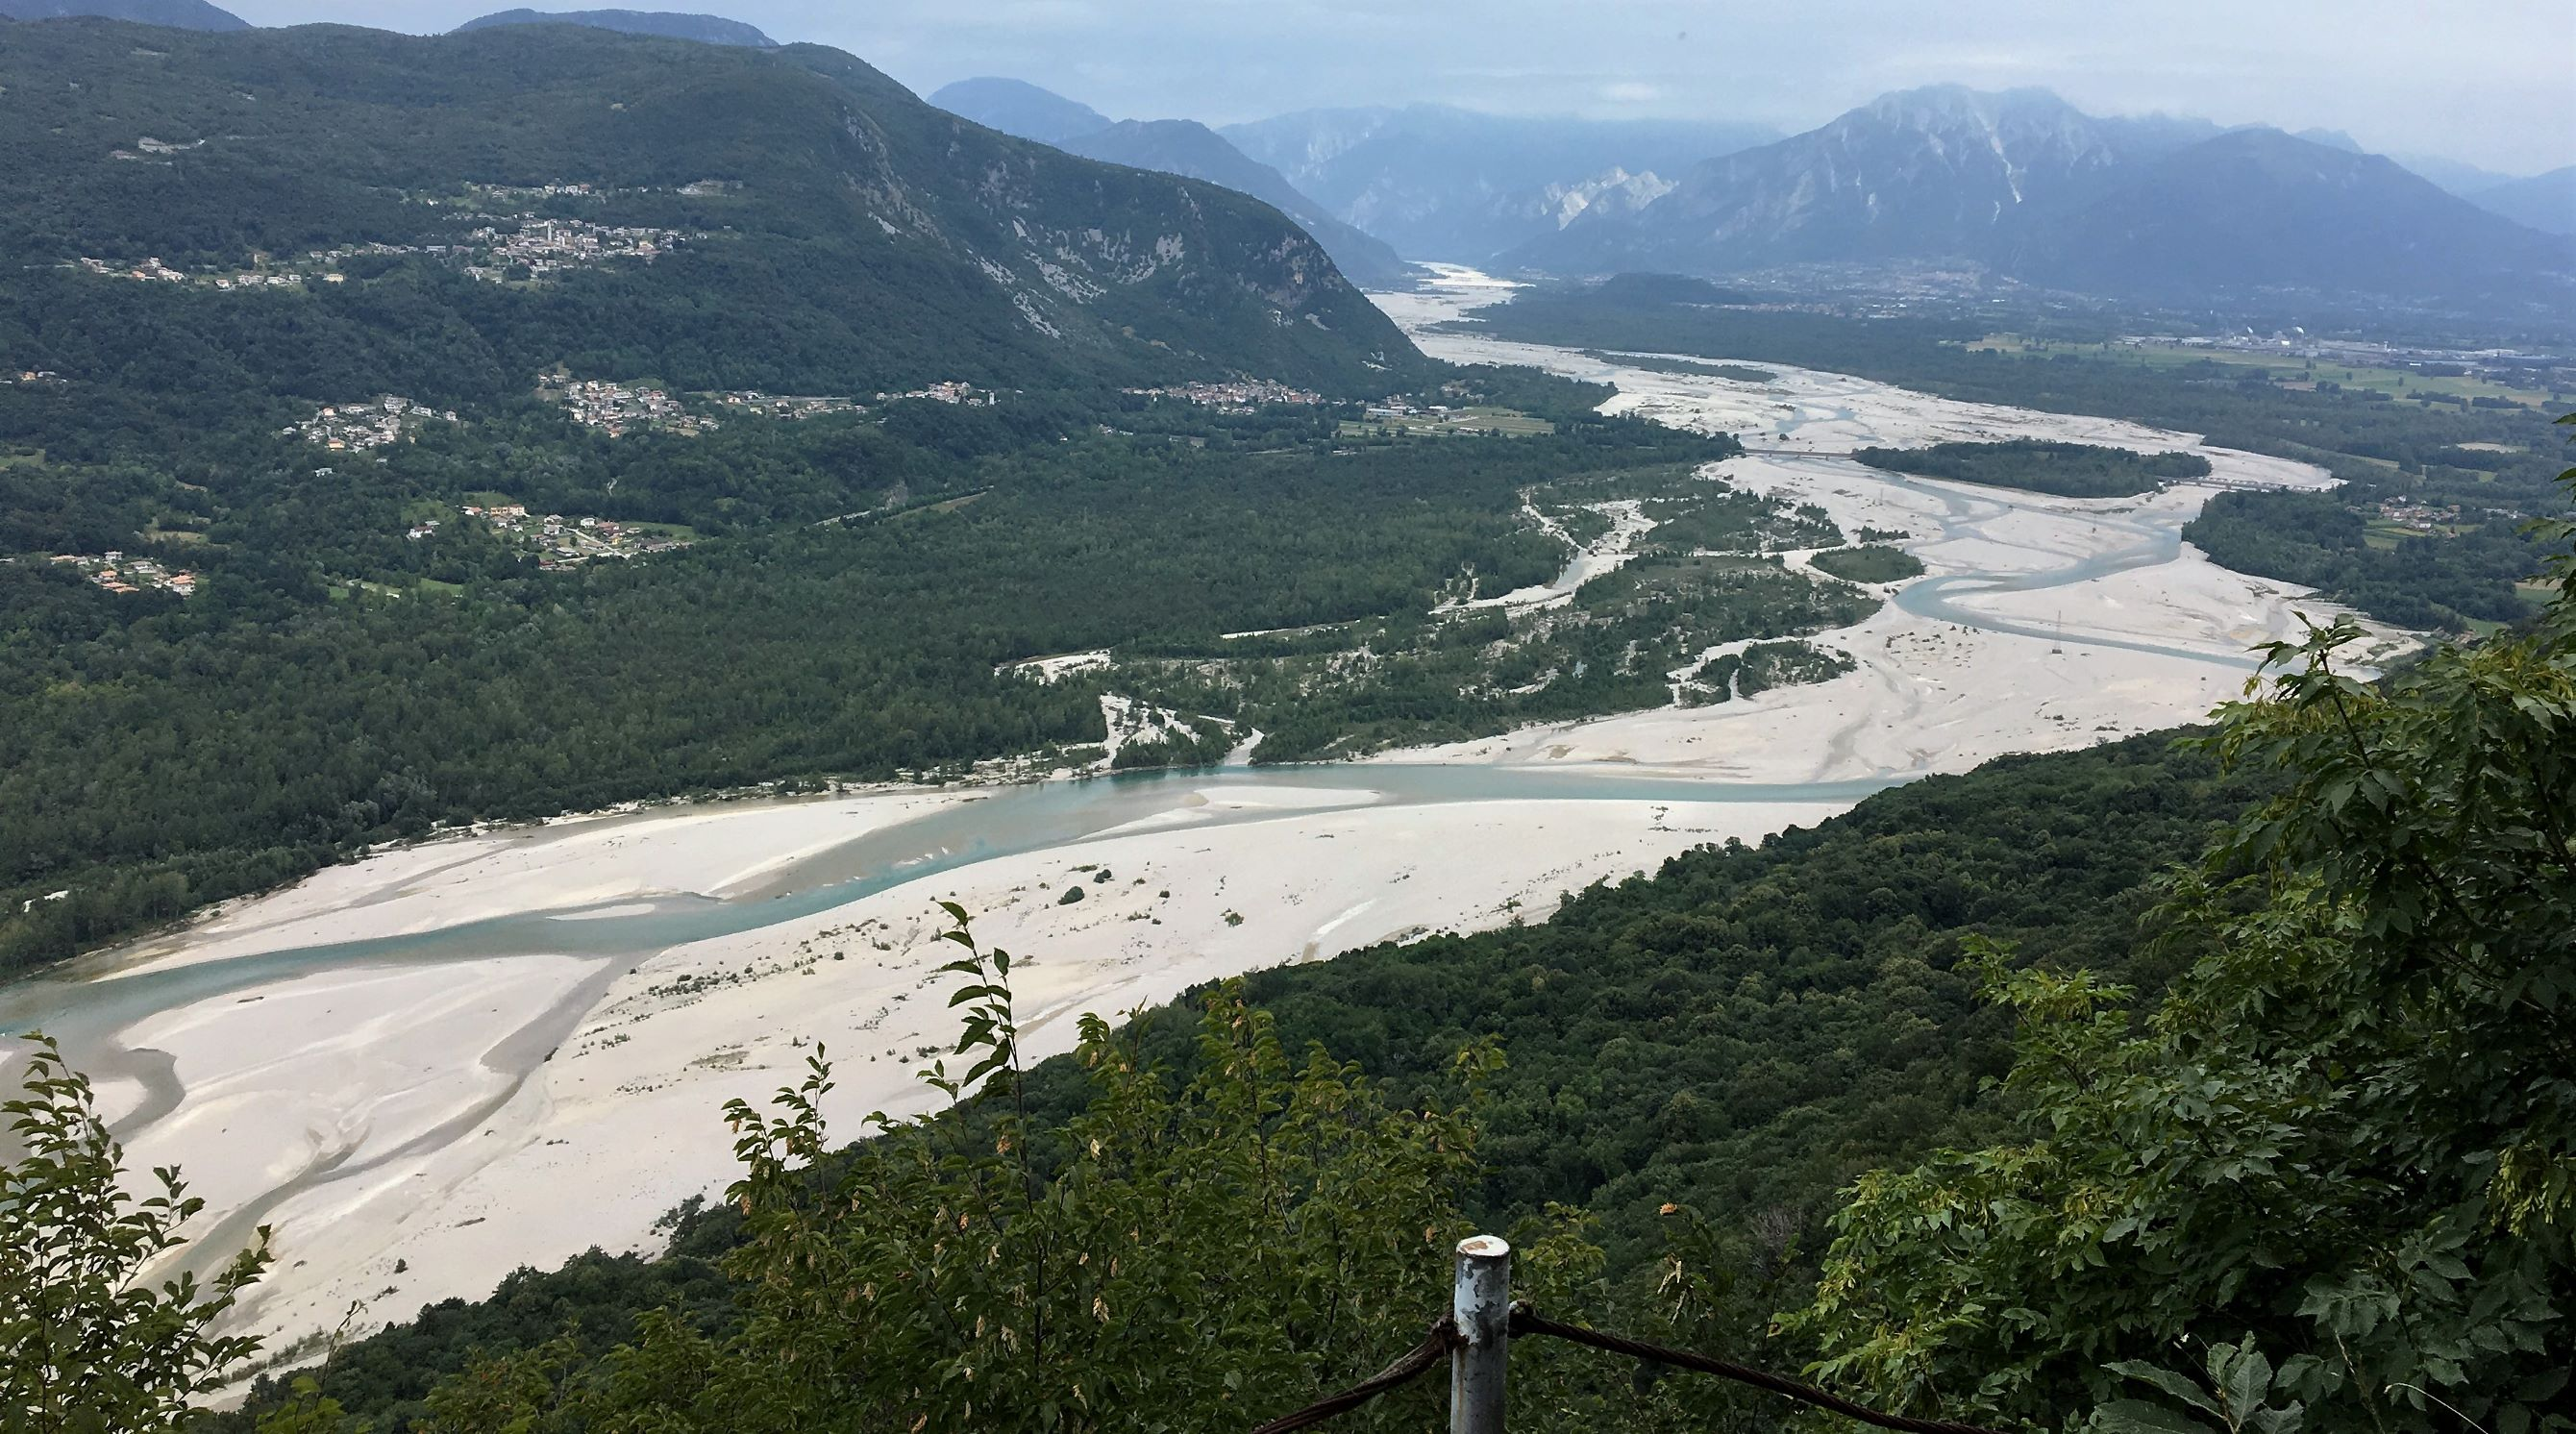
\includegraphics[width=\textwidth]{files/foto_flagogna.jpg}
	\caption[foto di un tratto del Tagliamento ripreso dal monte di Ragogna]{foto di un tratto del Tagliamento ripreso dal monte di Ragogna~(UD); l'acqua scorre da destra verso sinistra.
	}
	\label{fig:foto-ragogna}
\end{figure}



Questa prima figura mostra un fiume che scorre, libero, su un letto di ghiaia che forse pare essere decisamente più largo di quanto gli basterebbe. 
Dove sono gli argini? Il fiume può spostarsi? 
%
In mezzo alla figura si vedono numerose isole divise dal resto della vegetazione da canali abbandonati in ghiaia e sabbia. 
Come si formano? Rimangono inalterate al passare degli anni? 
%
Poco più in basso, dall'altra parte del canale, si intravedono degli arbusti proprio sulla ghiaia. 
Cresceranno fino a formare un'isola tanto vegetata quanto le vicine sue sorelle più a monte? O saranno spazzati via durante la prossima piena?

\medskip
Queste e altre cose si possono leggere da questa foto, così come da quella successiva. Tutte le domande hanno un carattere dinamico più o meno evidente: la loro risposta non la si può ottenere osservando una foto, che è statica, ma una sequenza di istanti successivi quale può essere un filmato.
Come racconta un professore, occorre sincronizzare i nostri orologi con quello del fiume; non solo, bisogna anche che indossiamo gli occhiali giusti per guardare i fenomeni alla scala in cui si possono vedere. Chi mai trarrebbe conclusioni effettive sulla vita di un albero se guardasse solo la sua foglia per pochi secondi, o se lo confrontasse su due immagini satellitari acquisite a distanza di diversi decenni?

\begin{figure}
	\centering
	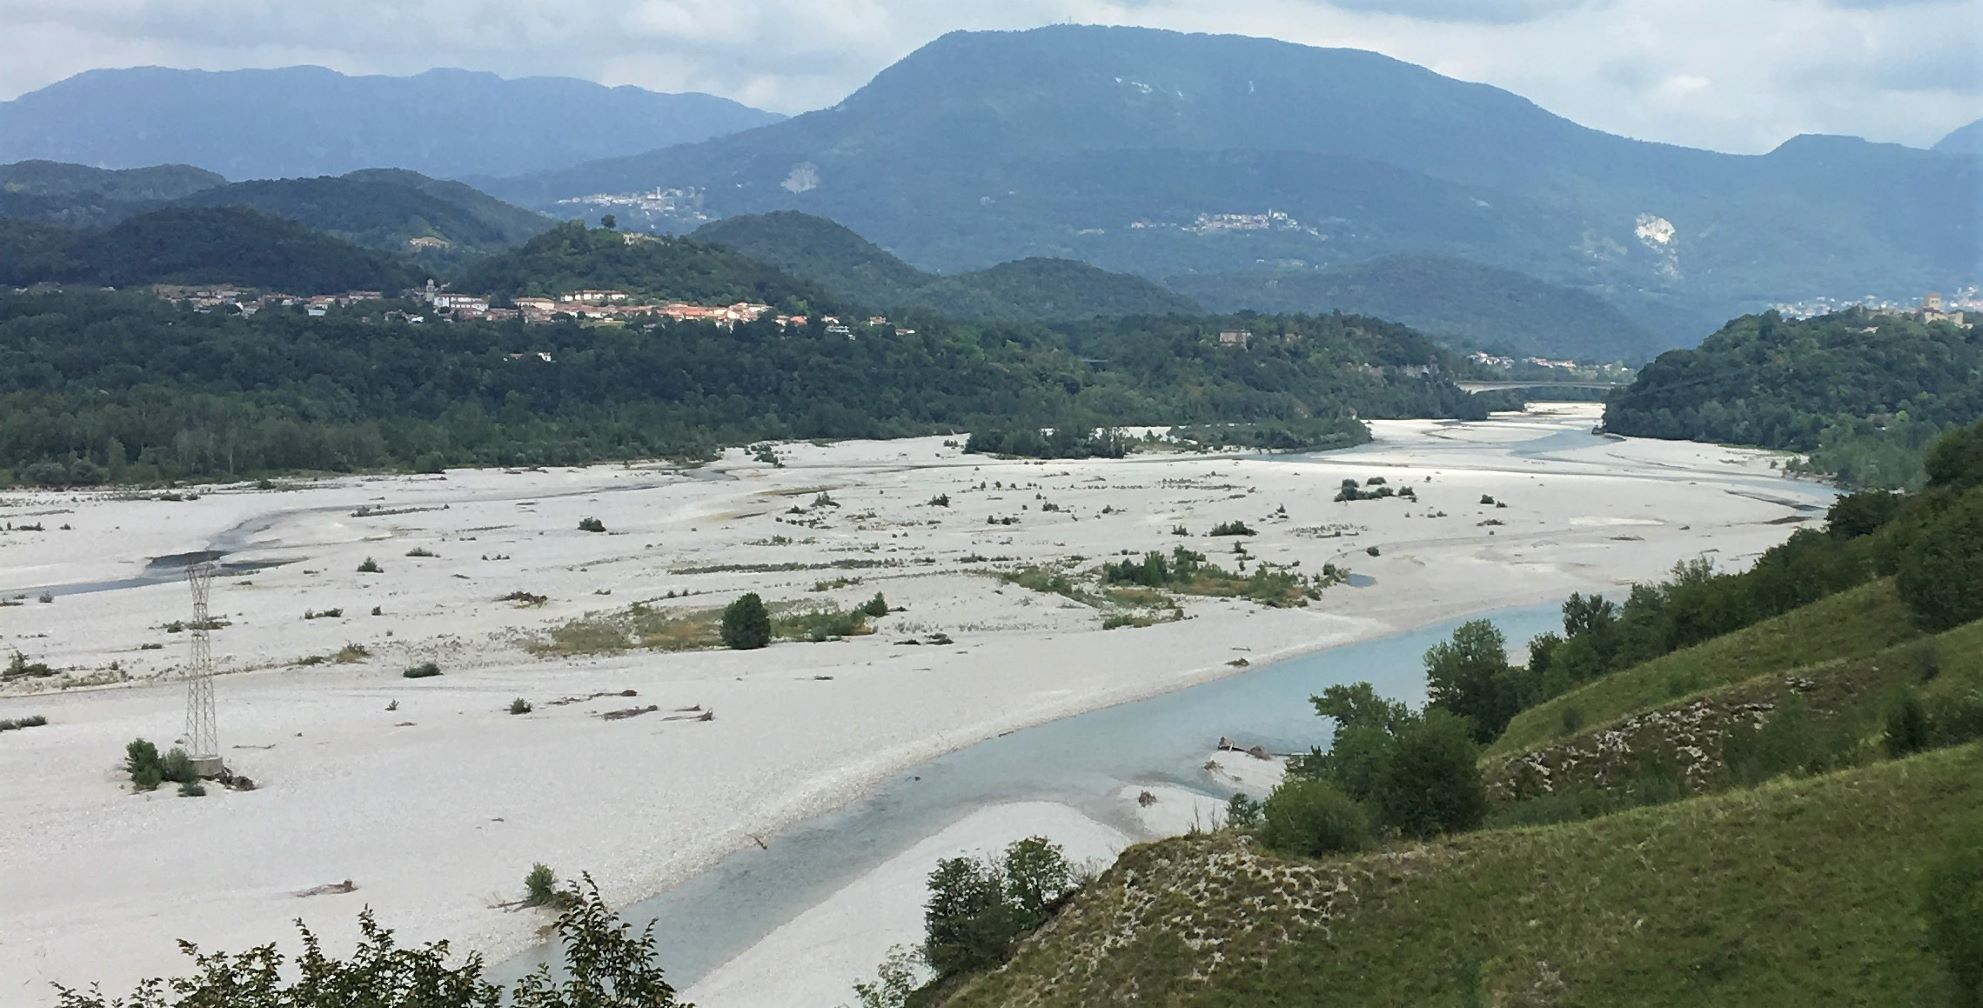
\includegraphics[width=\textwidth]{files/foto_terrazzo_valle_pinzano.jpg}
	\caption[foto di un tratto del Tagliamento ripreso dal terrazzo presso Aonedis~(UD)]{foto di un tratto del Tagliamento ripreso dal terrazzo presso Aonedis~(UD); l'acqua scorre da destra verso sinistra. 
	}
	\label{fig:foto-pinzano}
\end{figure}


Tra tutti i fiumi che ci sono nel nostro bel Paese, pochi di loro sono rimasti in condizioni “naturali”; l'alterazione ha apportato modifiche o ridotto l'entità dei processi che avevano luogo prima dell'intervento dell'uomo. 
Ad esempio, la costruzione di una diga a monte di un fiume può aver indotto nel corso degli anni un restringimento del suo alveo e ad un cambiamento della sua morfologia.
Ma in questo caso siamo fortunati: il Tagliamento può essere considerato un fiume alpino allo stato praticamente naturale.

Le domande che ho posto all'inizio nascono dalla curiosità che si può avere quando, dopo mesi di studio dei fenomeni che naturalmente avvengono nei fiumi, si incontra un fiume dove questi fenomeni possono accadere per davvero. Le domande trovano una risposta reale, comprovata da ciò che si vede quando si cammina sulla ghiaia, in mezzo alle isole, nei canali, e quando ci si tuffa nelle loro confluenze.

\medskip
La \cref{fig:confronto-imm-prefaz} mostra diversi processi che avvengono in questo fiume; questi, inutile ripeterlo, diventano apprezzabili solo dopo aver indossato gli occhiali e l'orologio giusti, cioè osservando da un'altezza di poche centinaia di metri da terra e confrontando immagini distanti pochi mesi. Ecco un'anteprima:
\begin{itemize}
	\item si vede subito che i canali migrano e si spostano durante gli anni; 
		difatti durante le piene più importanti tutto l'alveo si riempie di acqua e il fondo viene rimodellato;
	\item lo spostamento dei canali porta questi ad erodere lateralmente le isole, come si vede per l'isola in alto a sinistra in alveo; 
		il fiume quindi potrà trasportare non solo il materiale presente sul fondo, ma anche quello che erode dalle isole, sia ghiaia e sabbia che alberi;
	\item le isole possono espandersi da piccoli nuclei fino a unirsi, diventare più fitte e più resistenti all'erosione da parte dell'acqua, come si vede per la grande isola al centro della \cref{fig:confronto-imm-prefaz};
	\item l'erosione non risparmia le sponde, come si vede per la sponda a sinistra (in destra idrografica se si osserva il verso della corrente) la quale arretra di più di \SI{100}{\m} a causa delle piene che si susseguono nei tre anni di osservazione;
	\item l'erosione di isole e sponda produce moltissimo materiale legnoso (alberi sradicati) il quale si deposita poco più a valle della zona di erosione, come testimoniano i numerosi puntini scuri presenti sull'alveo asciutto; 
		se le condizioni sono adatte e se le piante sono in grado, è possibile che dai tronchi depositati crescano nuovi rami e radici; 
		questi tronchi diventano i nuclei di formazione di future isole;
	\item lo spostamento dei canali è limitato dalla presenza delle isole, che si configurano come ostacolo per la corrente anche durante le piene;
		difatti è difficile che il canale si possa spostare dove c'è l'isola in alto a destra, a meno che non riesca ad eroderla.
\end{itemize}

\begin{figure}
	\centering
	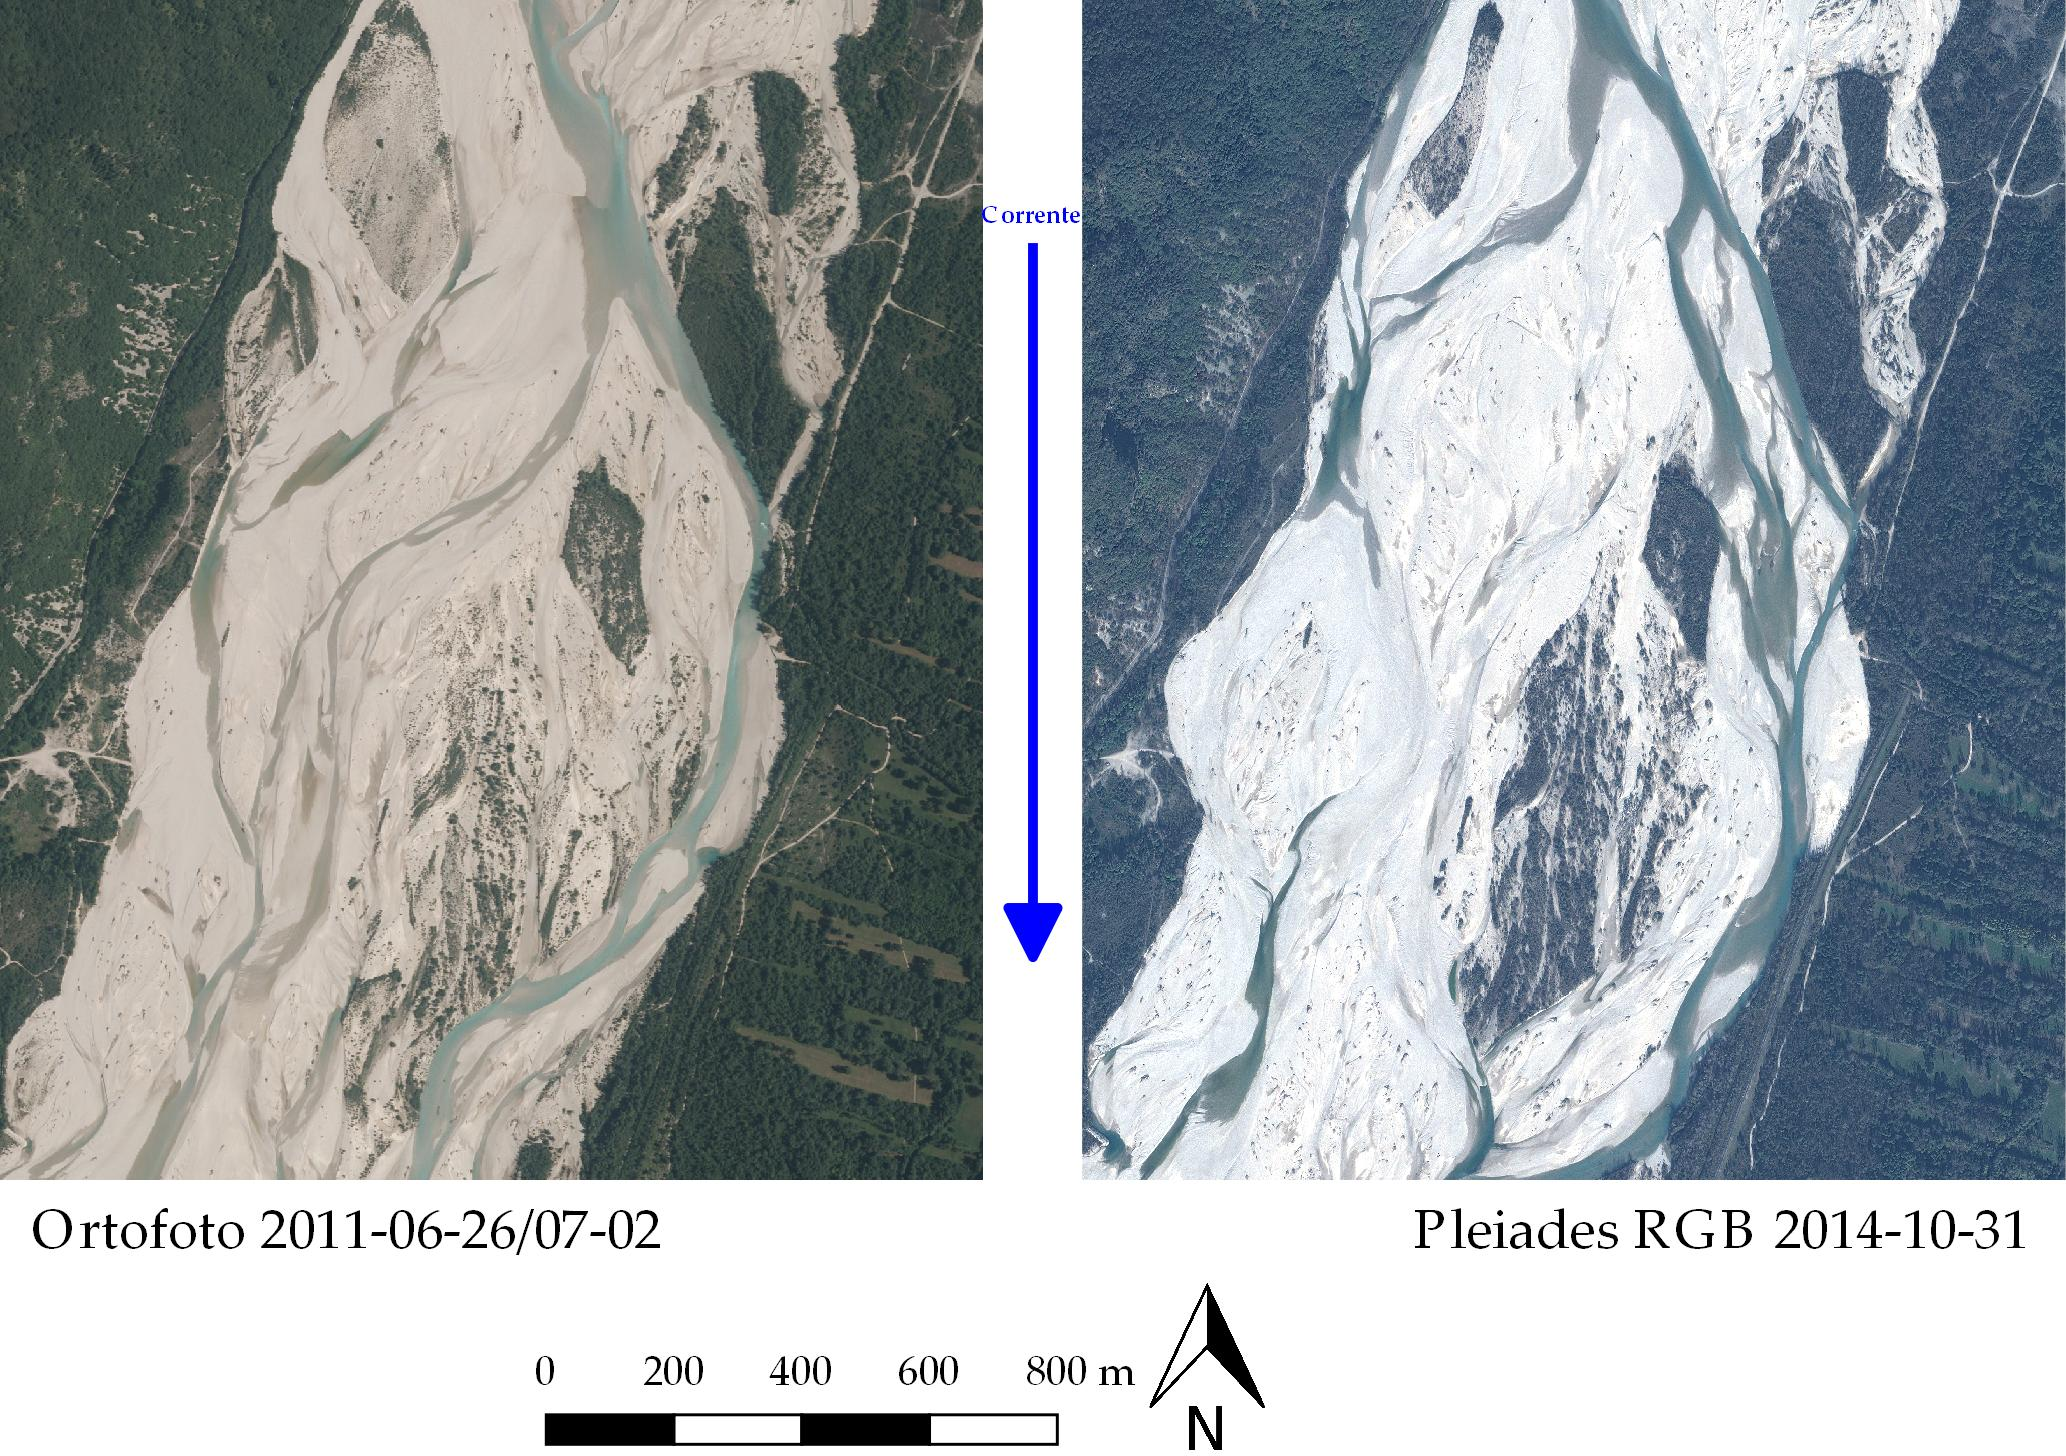
\includegraphics[width=\textwidth]{files/confronto_immagini_erosione_isole.jpeg}
	\caption[immagini di un tratto posto circa \SI{2}{\kilo\m} a monte del ponte di Cornino]{immagini di un tratto posto circa \SI{2}{\kilo\m} a monte del ponte di Cornino~(UD); l'ortofoto proviene dal Portale Cartografico Nazionale del Ministero dell'Ambiente.
	}
	\label{fig:confronto-imm-prefaz}
\end{figure}


Quante cose si possono osservare! In un fiume siffatto sono presenti numerosi altri fenomeni anche a scale diverse.
Ho raccontato quelli che mi interessano particolarmente e che sono oggetto di questa tesi: le dinamiche della vegetazione sulle isole e le dinamiche del legno depositato in alveo.

\medskip
A pensarci bene, non è sorprendente che in un sistema naturale la componente biologica influenzi fortemente quella fisica: i boschi consolidano i pendii e le foreste determinano la forma meandriforme di molti fiumi. Attraverso altri esempi ci si può convincere che le isole vegetate e i tronchi che rigettano in arbusti possano esercitare effetti su un fiume e viceversa. 
\\
E riflettendo ancora non è difficile osservare che queste interazioni solitamente possono indurre effetti positivi sia per l'ambiente che per l'essere umano: per portare qualche esempio, nel caso del Tagliamento si parla di biodiversità data da un mosaico in continuo cambiamento di ambienti diversi, di purificazione dell'acqua, del mantenimento di un microclima particolarmente adatto alla stagionatura del prosciutto di San Daniele (prodotto nell'omonimo paese poco distante) e di un luogo molto adatto per la ricreazione da parte delle persone (\cref{fig:bagnanti}).

Da questi fatti muovo i primi passi verso l'approfondimento dei processi che portano un fiume a modificarsi di continuo assieme all'ambiente in cui si colloca.


\begin{figure}[hb]
	\centering
	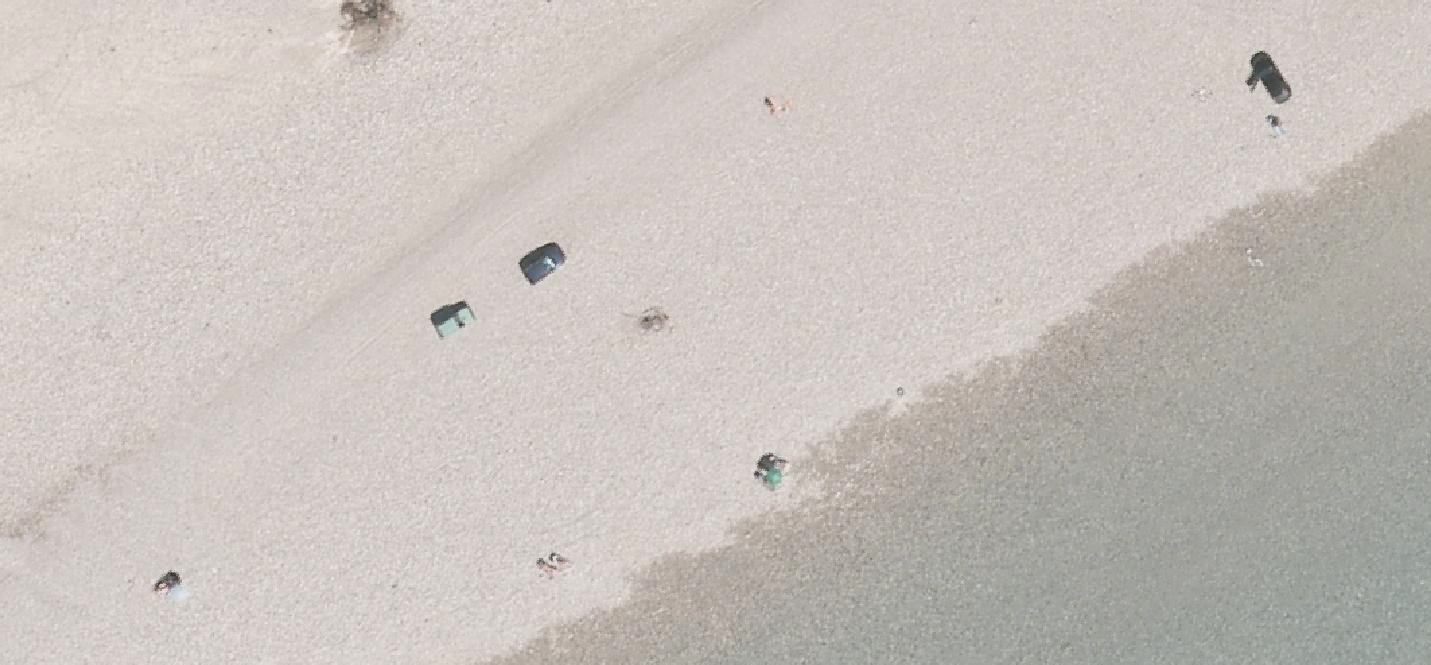
\includegraphics[width=\textwidth]{files/bagnanti.jpeg}
	\caption[bagnanti accanto ad un canale]{bagnanti accanto ad un canale ripresi con una immagine area del~2011, cortesemente fornita da Nicola Surian (Università degli studi di Padova).}
	\label{fig:bagnanti}
\end{figure}



%----------------------------------------------------------



%**********************************************************
%**********************************************************
\mainmatter
\chapter{Introduzione}
\section{L'area di studio: il Tagliamento}
\label{sec:descr-area-studio}
\paragraph{Inquadramento}
Nei fiumi a morfologia intrecciata dove l'impatto antropico non è intenso è possibile trovare isole nell'alveo dove il disturbo indotto dalle piene non è eccessivo;
queste si formano e accrescono nel periodo compreso tra eventi di piena di una certa entità, mentre vengono erose dagli eventi idrologici sufficientemente intensi \squarecites{Poff:1997}{Gurnell:2001-island-formation}.
La presenza delle isole ha un importante ruolo ecologico: la varietà spaziale e temporale di ambienti presenti (pozze d'acqua, sorgenti e canali separati da aridi sedimenti, zone con vegetazione bassa e rada alternate con isole fitte e mature che si modificano tra e in seguito alle piene) crea un mosaico in continuo cambiamento che sostiene una forte biodiversità \squarecites{Arscott:2002-habitat-dynamics}.
Inoltre, durante piene di piccola entità le piante influenzano l'accrescimento delle forme fluviali attraverso la ritenzione di sedimenti e materiale legnoso sia morto che vivo, inducendo così la successiva colonizzazione da parte di altre piante e la rimodellazione dei canali \squarecite{Gurnell:2006-omega}.


Il Fiume Tagliamento, situato nel Nord-Est italiano, è uno dei pochi fiumi alpini allo stato quasi naturale che presenta queste caratteristiche. 
Sono stati effettuati interventi di ingegneria fluviale, come arginature, derivazioni, pennelli, estrazione di ghiaia, sia in tratti posti a monte che in altri posti a valle; la loro entità è comunque tanto limitata da poter parlare di “contesto non gestito”.
\\
Difatti il Tagliamento presenta un regime idrologico non alterato, con piene frequenti ed imprevedibili dovute all'alta piovosità nel bacino \squarecites{Mosetti:1983}{Bertoldi:2009-2m} e alla limitata presenza di bacini di regolazione (solo il \SI{3}{\percent} dell'area drenante del bacino è intercettata da dighe \squarecite{Sitzia:2016-d50});
è stato suggerito che è possibile formulare previsioni accurate di un evento di piena solamente nelle 5 ore precedenti \squarecite{Arscott:2002-habitat-dynamics}. 
Inoltre, le sponde e l'alveo sono colonizzate da ampie porzioni di vegetazione riparia lungo quasi tutto il suo corso. 
Questi fatti indicano che le attività umane sul Tagliamento non sono tali da aver alterato o da alterare il regime del fiume.

Il bacino idrografico del Tagliamento, ampio circa~\SI{2900}{\kilo\m\tothe{2}}, si estende tra le province di Belluno, Udine, Pordenone e Venezia.
Il suo corso di circa~\SI{170}{\kilo\m} presenta morfologia intrecciata (\emph{braided}) con canali multipli separati da barre e isole.
Nelle parti montane è confinato dai versanti; 
nella parte planiziale è libero, con tratti larghi diverse centinaia di metri, se non più di \SI{1}{\kilo\m};
a qualche decina di chilometri dalla foce il fiume si restringe assumendo prima una forma transizionale monocursale con larghezza sui \SIrange[range-phrase={-}]{300}{200}{\m} nei pressi di Madrisio~(UD);
infine diventa meandriforme a Latisana~(UD) (larghezza intorno ai \SI{100}{\m}) fino alla foce, situata tra Bibione~(VE) e Lignano~(UD).
\\
Insieme alla variazione della morfologia del fiume si assiste ad un cambiamento nella granulometria: mentre la ghiaia predomina nella parte intrecciata ($d_{50} = \SI{4}{\centi\m}$ \squarecites{Bertoldi:2010-d50}{Sitzia:2016-d50}), a partire dal tratto meandriforme si trova solo sabbia sul fondo.
Questo mutamento di materiale trasportato riflette la riduzione della pendenza che si osserva dal tratto transizionale monocursale e che giustifica il passaggio da fiume “in ghiaia” a fiume “in sabbia”.
\\
Le precipitazioni sono mediamente di circa \SI{2000}{\mm} all'anno con forti variazioni locali; i minimi di precipitazione si registrano durante l'inverno, mentre i massimi in primavera e in autunno.
Si assiste anche ad eventi di breve durata e particolarmente intensi.
Il regime fluviale che ne risulta è di tipo \emph{flashy} pluvio-nivale con piene brevi ed intense così come piene di diversi giorni di durata.

Il tratto studiato è quello intrecciato multicanale compreso tra Tolmezzo~(UD) e Madrisio~(UD) (\cref{fig:overview,fig:overview-sat}). 
%
\begin{figure}
	\centering
	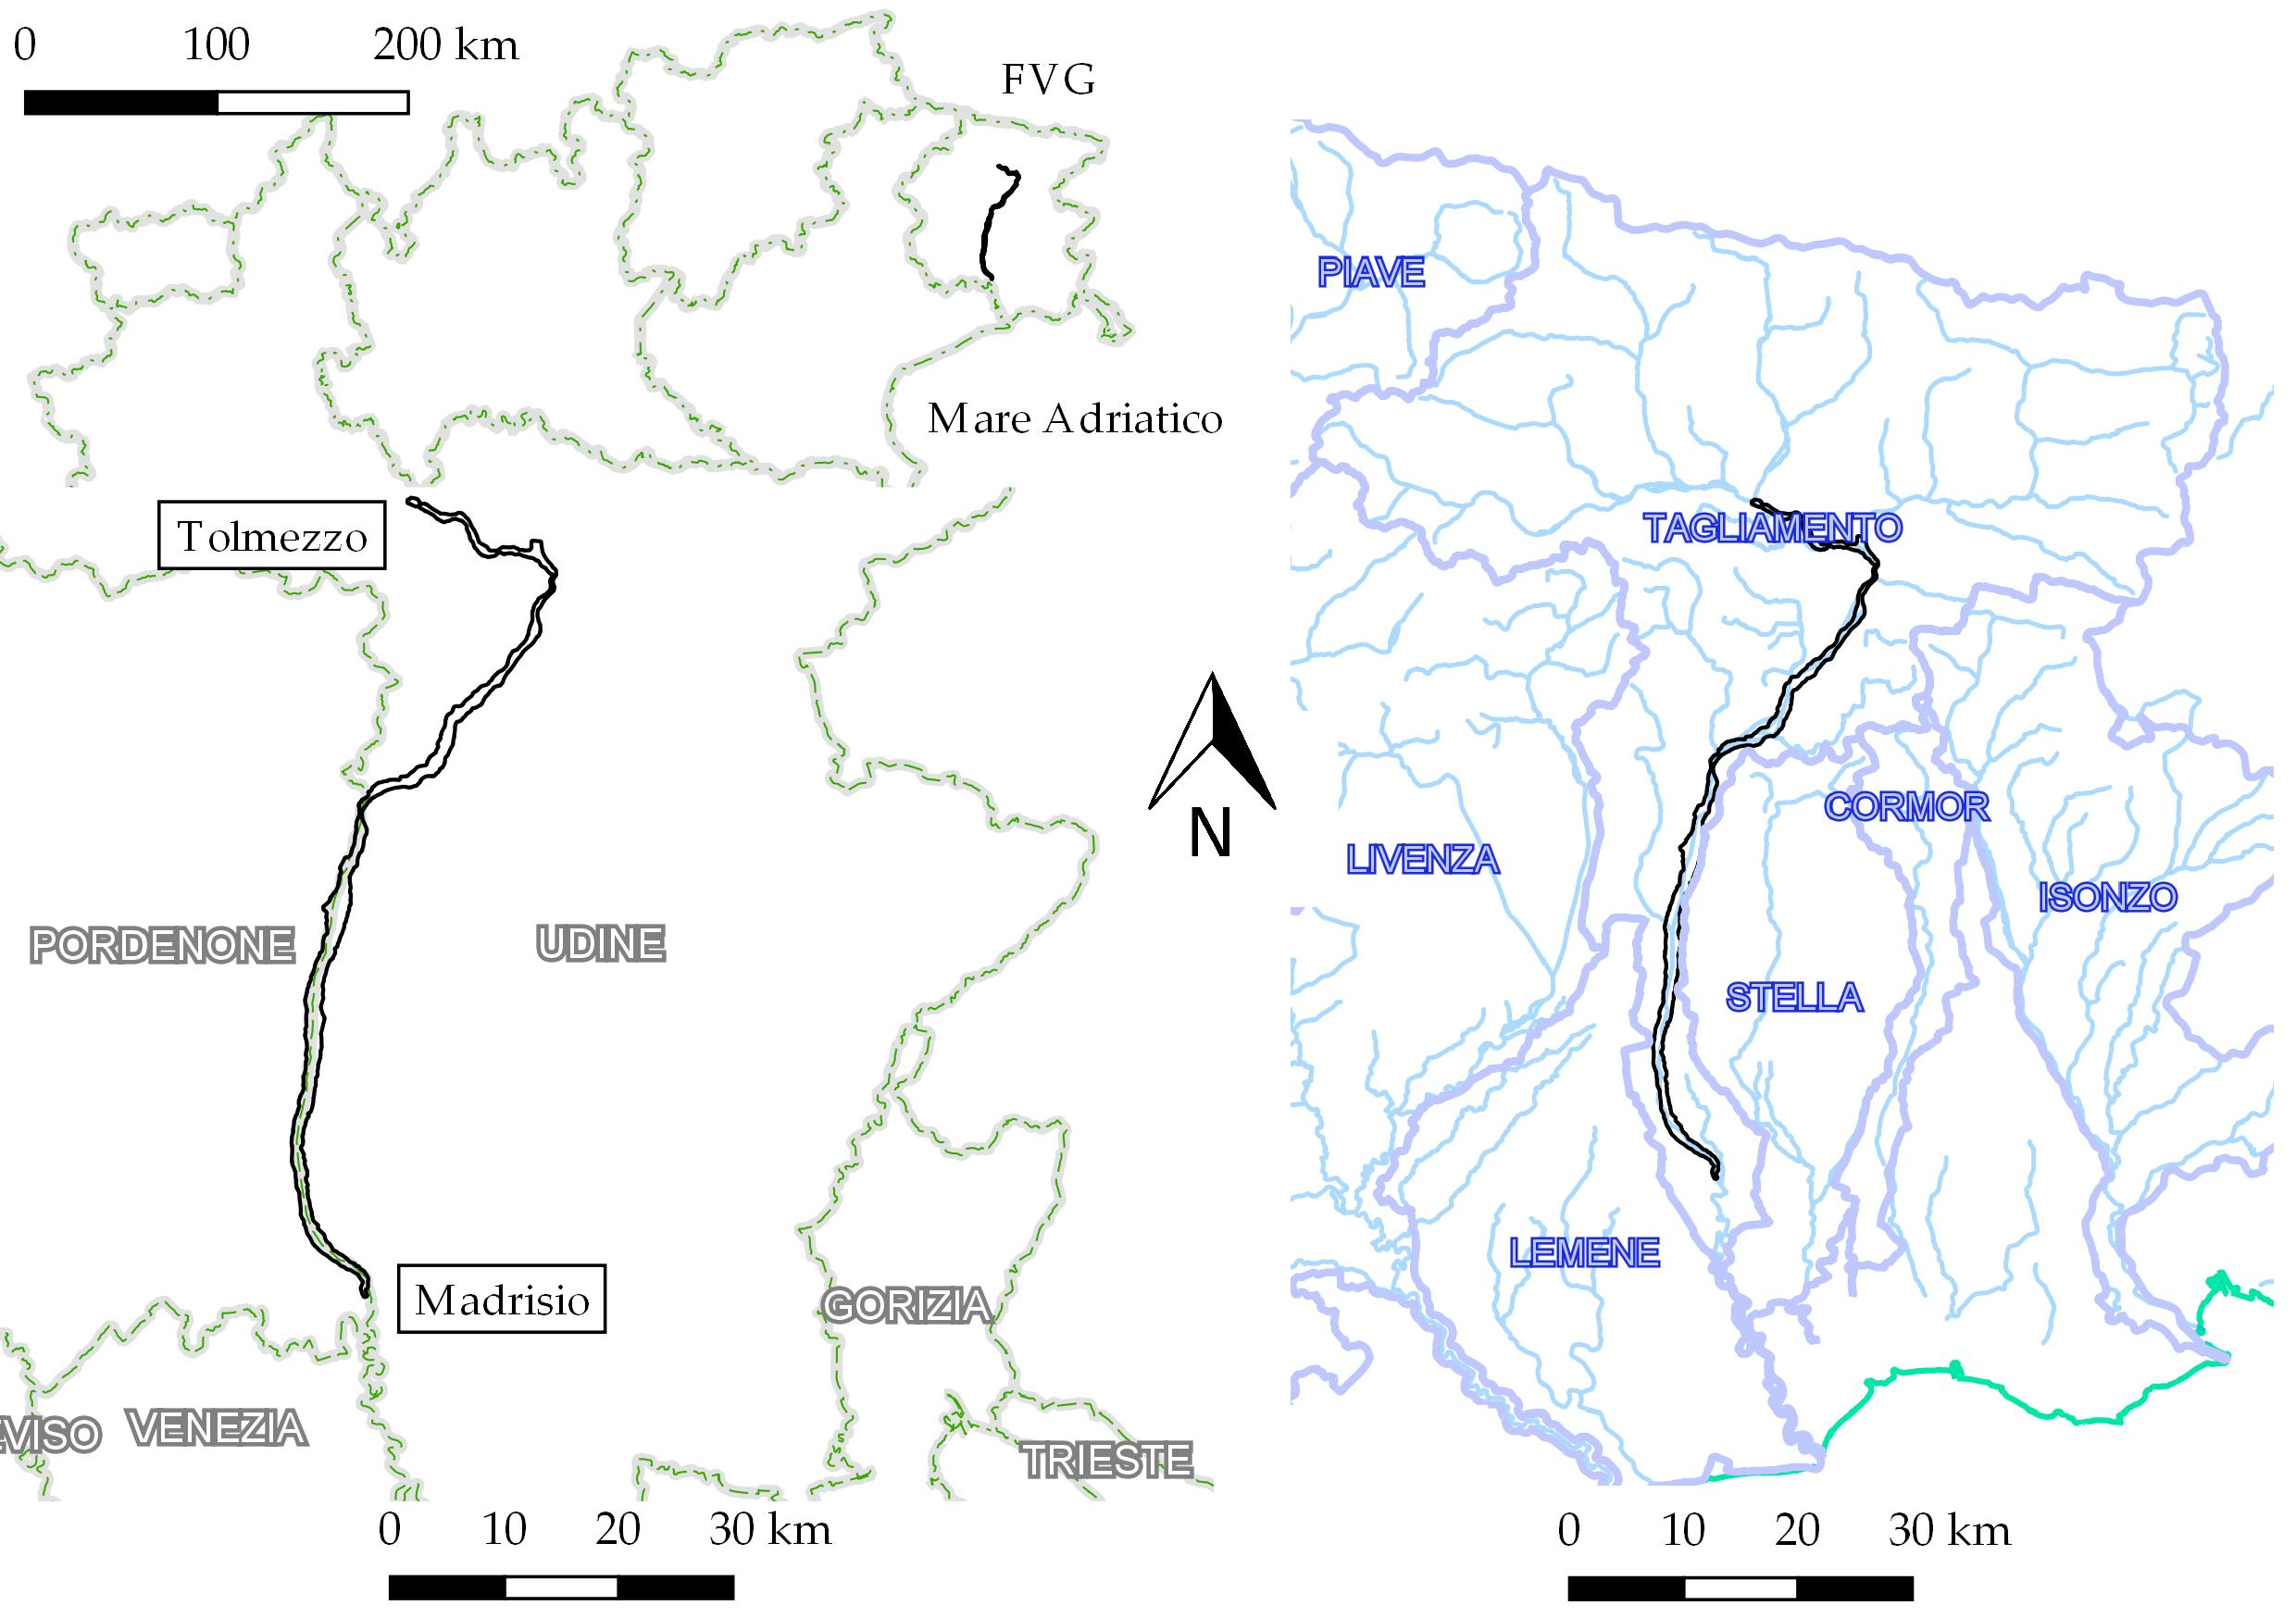
\includegraphics[width=\textwidth]{files/overview.jpeg}
	\caption[inquadramento dell'area di studio]
		{inquadramento dell'area di studio (poligono nero); a sinistra è mostrata l'Italia settentrionale (in alto) e un ingrandimento delle province e degli estremi dell'area di studio (in basso); a destra si vede il bacino idrografico del Tagliamento e di altri fiumi nelle vicinanze (in blu), il reticolo idrografico (in azzurro) e la linea di costa (in verde acqua). I tematismi provengono dal Portale Cartografico Nazionale del Ministero dell'Ambiente.}
	\label{fig:overview}
\end{figure}
%
\begin{figure}
	\centering
	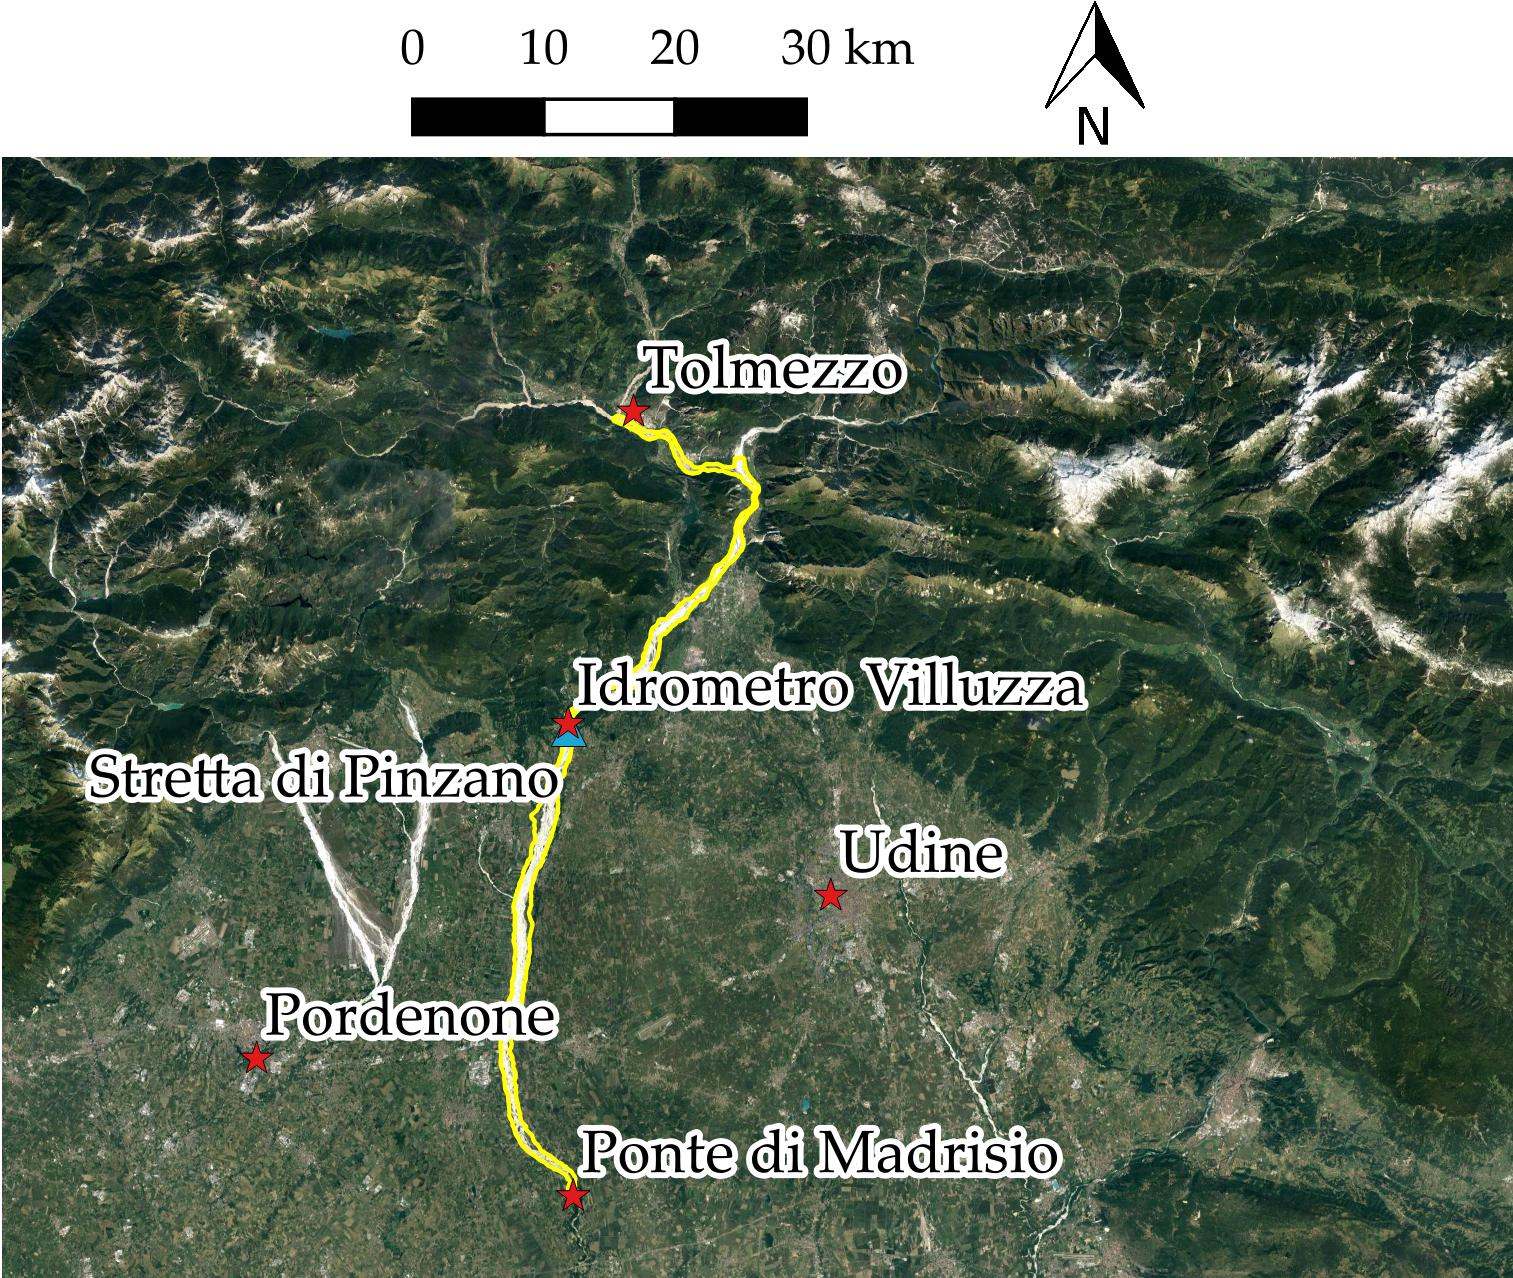
\includegraphics[width=\textwidth]{files/overview_tratto_sat.jpeg}
	\caption[inquadramento dell'area di studio]{inquadramento dell'area di studio (contornata in giallo) assieme ad alcune zone di interesse.
	\\
	Map data: Google, Digital Globe.}
	\label{fig:overview-sat}
\end{figure}
%
\\
L'area di studio è stata suddivisa manualmente in 23~tratti al fine di avere un maggior dettaglio spaziale delle dinamiche di vegetazione (\cref{fig:23-tratti}). 
Questi tratti sono stati selezionati in modo da possedere caratteristiche omogenee per portata e crescita della vegetazione; 
pertanto confluenze di immissari, bruschi restringimenti o allargamenti, inizio di pronunciato \emph{upwelling} o \emph{downwelling} ed evidenti cambiamenti di morfologia fluviale sono stati gli elementi per individuare i 23~tratti.
%
\begin{figure}
	\centering
	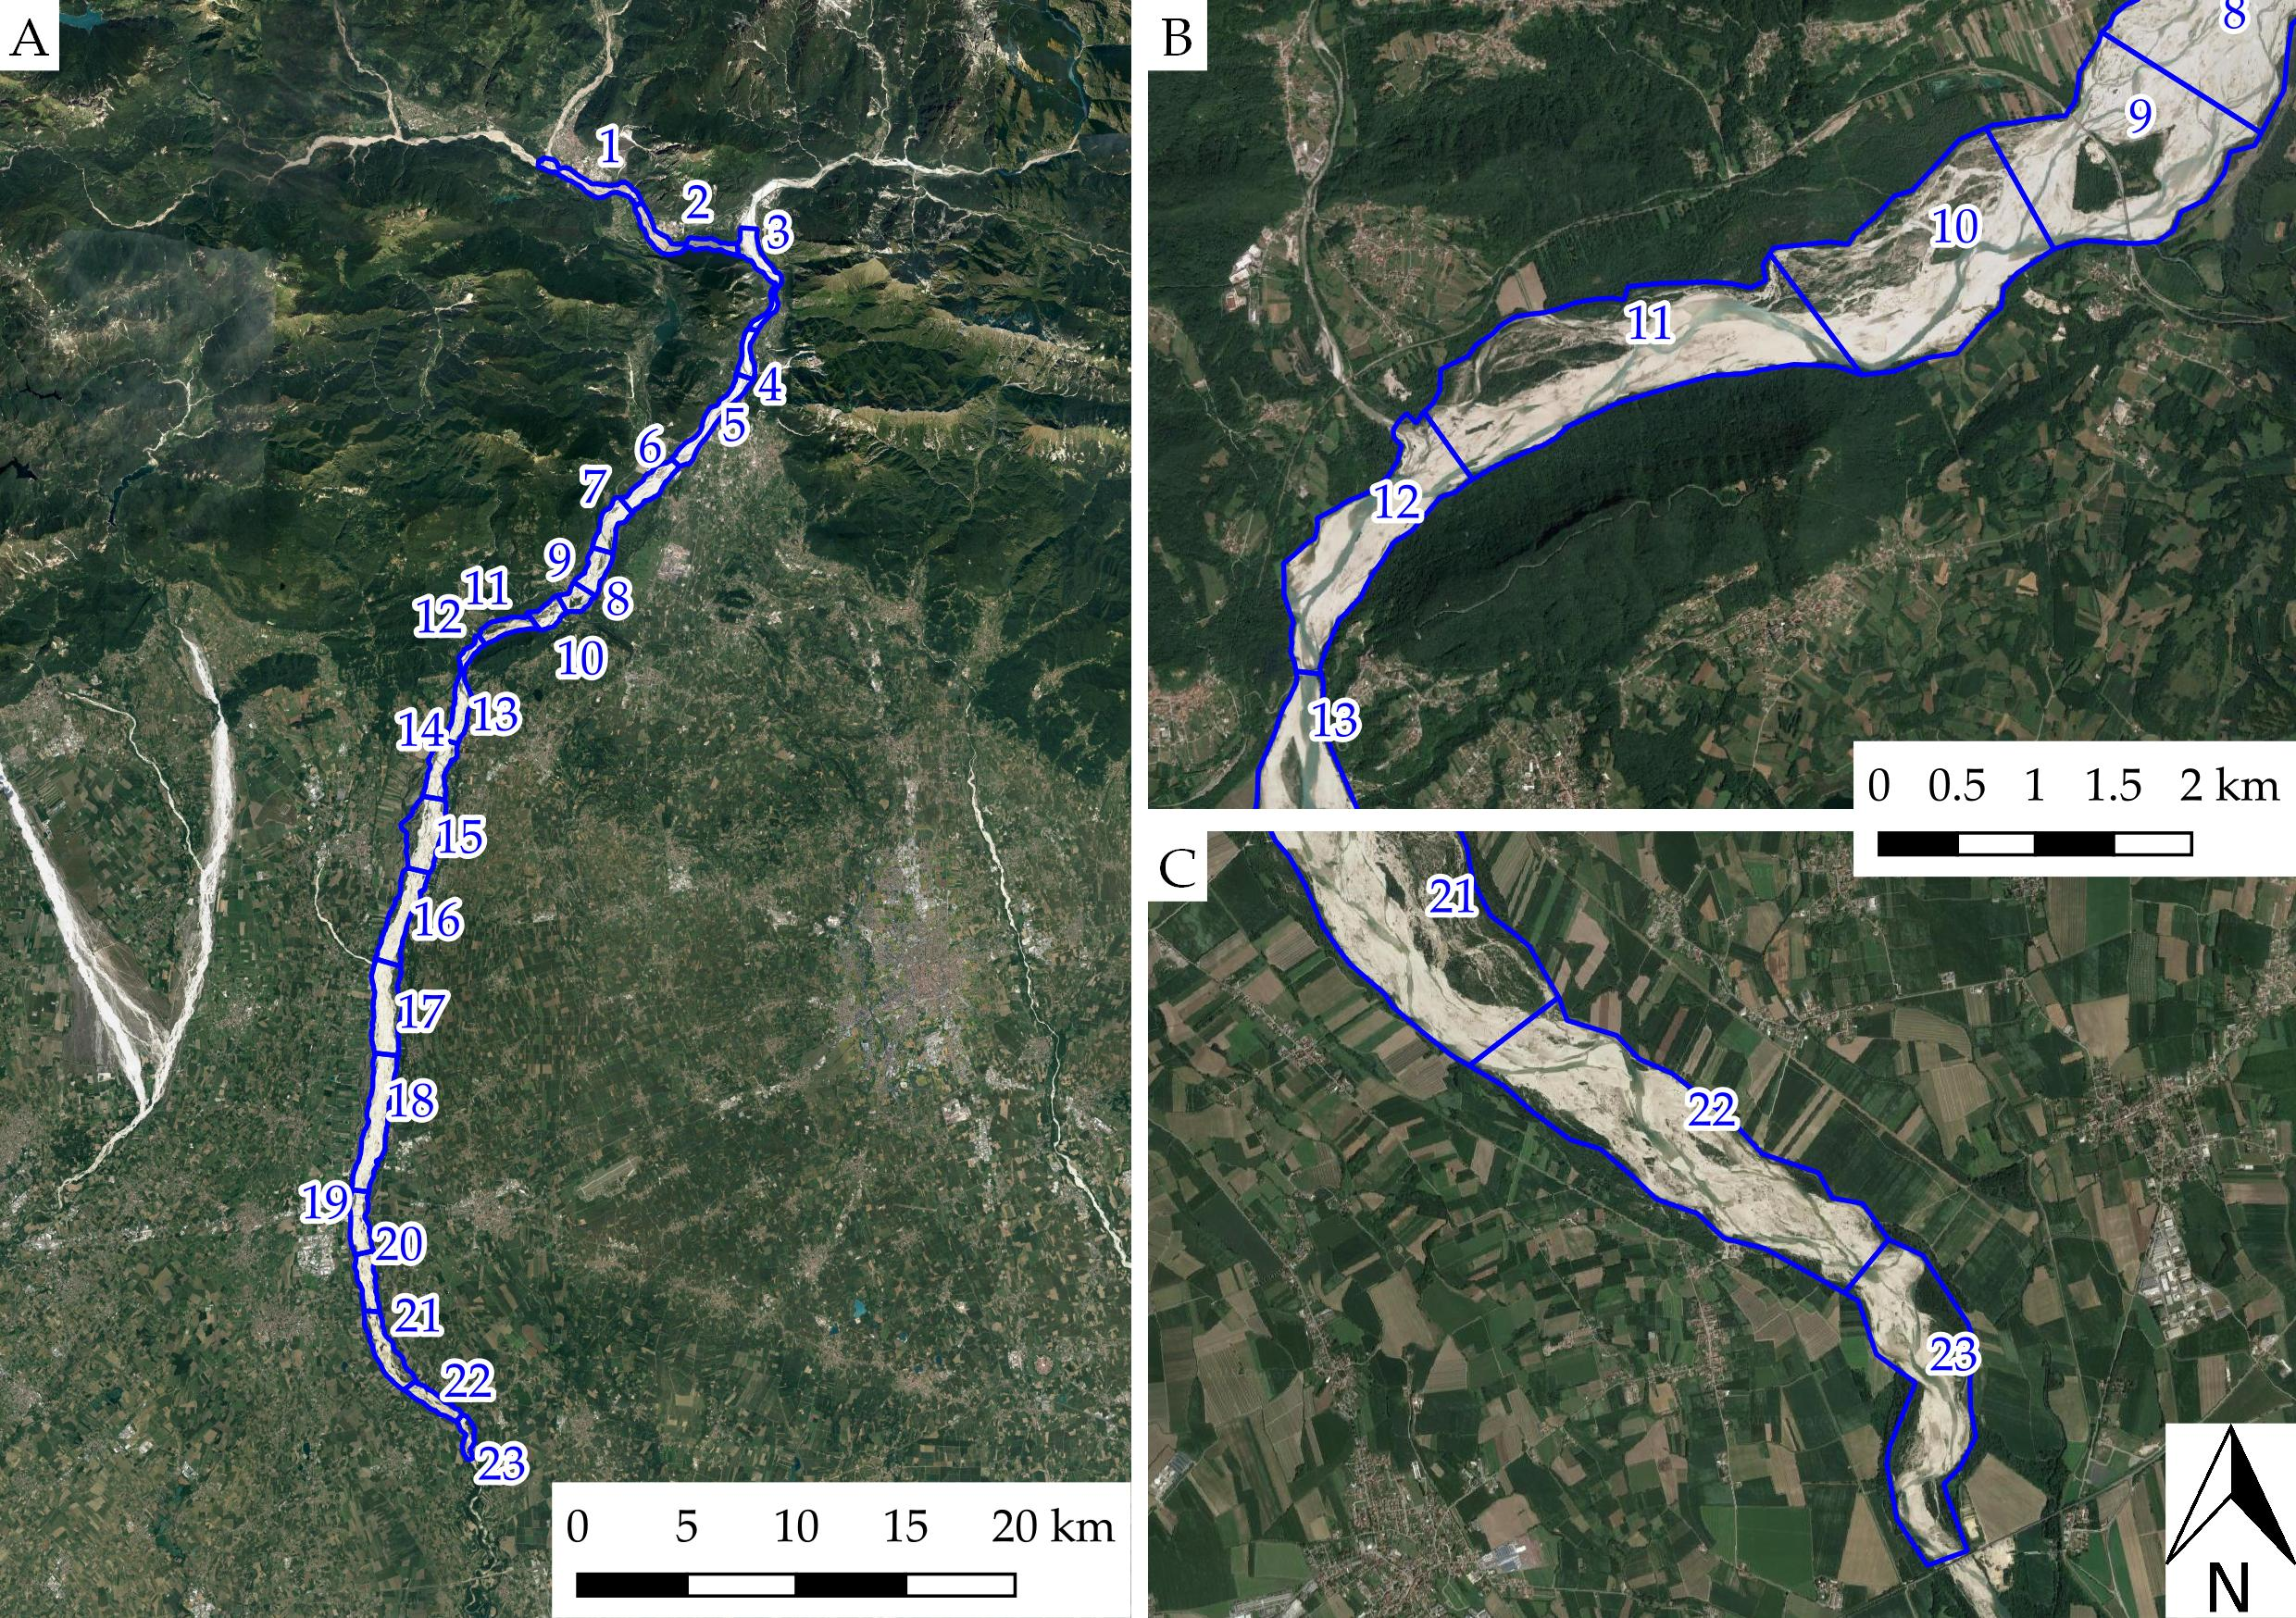
\includegraphics[width=\textwidth]{files/tutti_23_tratti.jpeg}
	\caption[immagine dei 23 tratti in cui è suddivisa l'area di studio]{immagine dei 23 tratti in cui è suddivisa l'area di studio (figura~A); la sezione di monte del tratto~1 corrisponde a Tolmezzo, la sezione di valle del tratto~23 corrisponde al ponte di Madrisio. A destra sono mostrati ingrandimenti dei tratti presso l'isola di Cornino (tratto~9) e la stretta di Pinzano (tra il tratto~12 e il~13) (figura~B) e nei tratti dove la morfologia diventa transizionale poco a monte di Madrisio (tratti~22 e~23) (figura~C).
	\\
	Map data: Google, Digital Globe.}
	\label{fig:23-tratti}
\end{figure}


\paragraph{Connessione con la falda}
Nel tratto di studio nei pressi del paese di Pinzano al Tagliamento~(PN) è presente una stretta causata dall'affioramento di strati rocciosi che riduce la larghezza da diverse centinaia di metri a circa \SI{130}{\m}.
Questo restringimento, congiuntamente all'innalzamento dello strato di roccia che si trova sotto il letto del fiume, induce variazioni longitudinali nel livello di falda nel materasso alluvionale.
L'acqua filtrante da monte risale in alveo sotto forma di sorgenti diffuse: si assiste al fenomeno dell'\emph{upwelling}.
A valle della stretta, dove l'alveo non è più confinato e il letto roccioso sprofonda nel sottosuolo, l'acqua torna ad infiltrarsi nel materasso ghiaioso (\emph{downwelling}) tanto da portare il fiume in condizioni di secca in certi tratti quando non ci sono piene.
\\
L'\emph{upwelling} e il \emph{downwelling} sono fenomeni rilevanti durante i periodi di magra: certi tratti a valle della stretta di Pinzano possono essere in condizioni di secca, privi completamente di acqua, la quale scorre tutta nel sottosuolo e riemerge presso la “Linea delle risorgive” \squarecite{Mosetti:1983}, quando la morfologia fluviale diventa transizionale pochi chilometri a monte del ponte di Madrisio.
\\
Durante le piene questi fenomeni sono invece irrilevanti: l'acqua che emerge o che si infiltra contribuisce minimamente alla portata fluente.
\\
Il moto di infiltrazione contribuisce al mantenimento di una forte biodiversità caratteristica dell'ambiente fluviale, oltre a permettere una costante purificazione dell'acqua fluente in periodi di magra.

\paragraph{Affluenti}
Nel tratto di studio vi sono diversi affluenti (\cref{fig:affluenti}); vengono qui elencati da monte (Tolmezzo) fino a valle (Madrisio):
%
\begin{itemize}
	\item poco a valle di Tolmezzo c'è il Fella in sinistra idrografica (\SI{706}{\kilo\m\tothe{2}});
	\item all'altezza del paese di Venzone~(UD), in sinistra idrografica, sfocia il torrente Venzonassa (\SI{39}{\kilo\m\tothe{2}});
	\item qualche chilometro a monte del paese di Cornino~(UD) in destra idrografica c'è il Leale (\SI{100}{\kilo\m\tothe{2}}), che ha sempre acqua fluente poiché riceve lo scarico della centrale idroelettrica che sfrutta il lago di Cavazzo; questo raccoglie le acque della parte montana del Tagliamento attraverso opere idrauliche;
	\item in corrispondenza dell'isola di Cornino in sinistra idrografica il Ledra (\SI{75}{\kilo\m\tothe{2}}) riporta nel corso del Tagliamento sia le acque che si sono infiltrate nella piana di Osoppo~(UD) \squarecite{Mosetti:1983} sia quelle intercettate dalla presa di Ospedaletto~(UD);
	\item immediatamente a monte della stretta di Pinzano in destra idrografica si getta l'Arzino (\SI{123}{\kilo\m\tothe{2}});
	\item infine, una decina di chilometri più a valle della stretta in destra idrografica si incontra il Cosa (\SI{160}{\kilo\m\tothe{2}}).
\end{itemize}
%
\begin{figure}
	\centering
	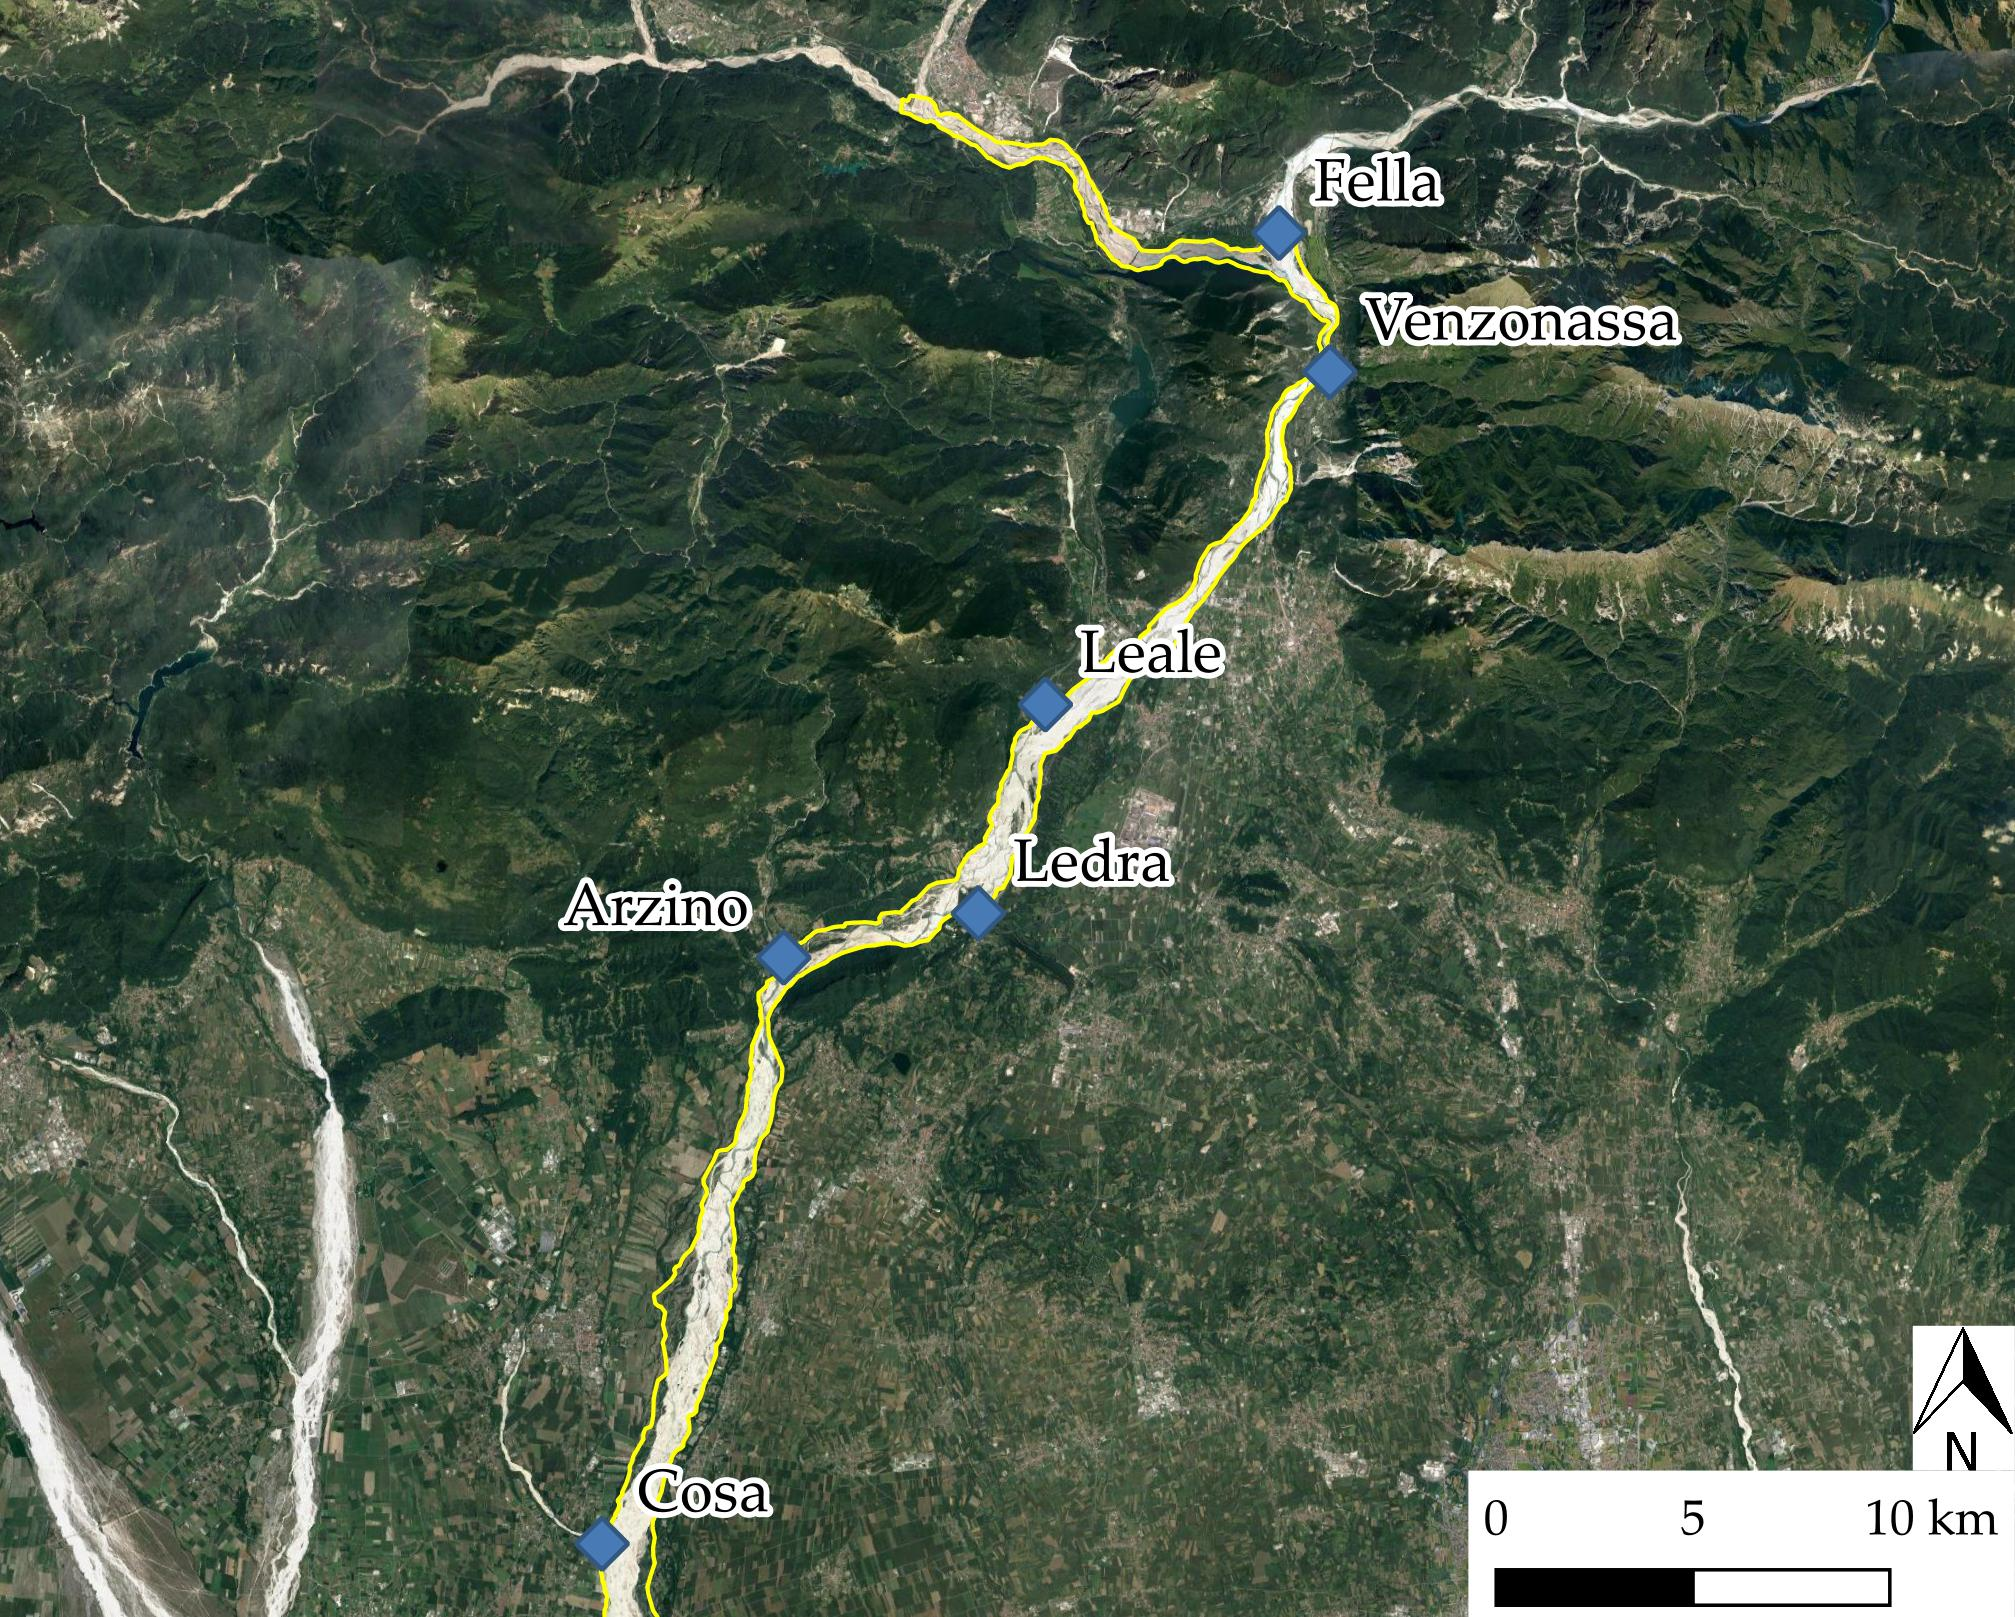
\includegraphics[width=\textwidth]{files/overview_affluenti.jpeg}
	\caption[principali affluenti nel tratto oggetto di studio]{principali affluenti nel tratto oggetto di studio (contornato in giallo); i rombi indicano i punti dove gli affluenti confluiscono nel Tagliamento.
	\\
	Map data: Google, Digital Globe.}
	\label{fig:affluenti}
\end{figure}
%
Il contributo di questi affluenti in termini di portata non è trascurabile; qualche decennio fa è stata evinta una relazione empirica tra l'area drenante di ogni bacino del Friuli Venezia Giulia \si{[\m\tothe{2}]} e la portata massima registrata in alcuni anni prima del 1950 \si{[\m\tothe{3}\per\s]} \squarecite{Mosetti:1983} che mostra l'evidente importanza degli affluenti:
%
\begin{equation}
	\label{eq:area-portata-mosetti}
	Q = 0.04598 \, A^{0.9546}	\quad	.
\end{equation}
%
Il limite di tale formula risiede nella determinazione delle portate utilizzate per la sua taratura; tuttavia la relazione fornisce la chiara indicazione che la portata in una sezione è all'incirca proporzionale all'area drenante sottesa.
\\
Si ritiene pertanto che conoscere il livello d'acqua in un punto del Tagliamento sia sufficientemente rappresentativo per descrivere qualitativamente l'entità di una piena in tutto il tratto di studio; per ottenere informazioni quantitative sulla portata fluente durante eventi di piena si assume che questa sia proporzionale all'area drenante in ogni sezione del fiume.

\paragraph{Dinamiche vegetazionali}
Nel fiume sono presenti numerose isole, composte prevalentemente da ontani bianchi \emph{Alnus incana} nei tratti montani (oltre l'area di studio), pioppi \emph{Populus nigra} e numerose specie di salice \emph{Salix spp.} nei tratti intermedi e vallivi.
Un'isola è un'area discreta e ben definita dell'alveo ricoperta da vegetazione e circondata da ghiaia o da canali (\cref{fig:esempio-isola}) \squarecites{Gurnell:2001-island-formation}{Bertoldi:2009-2m}.
%
\begin{figure}
	\centering
	\begin{subfigure}[b]{0.37\textwidth}
		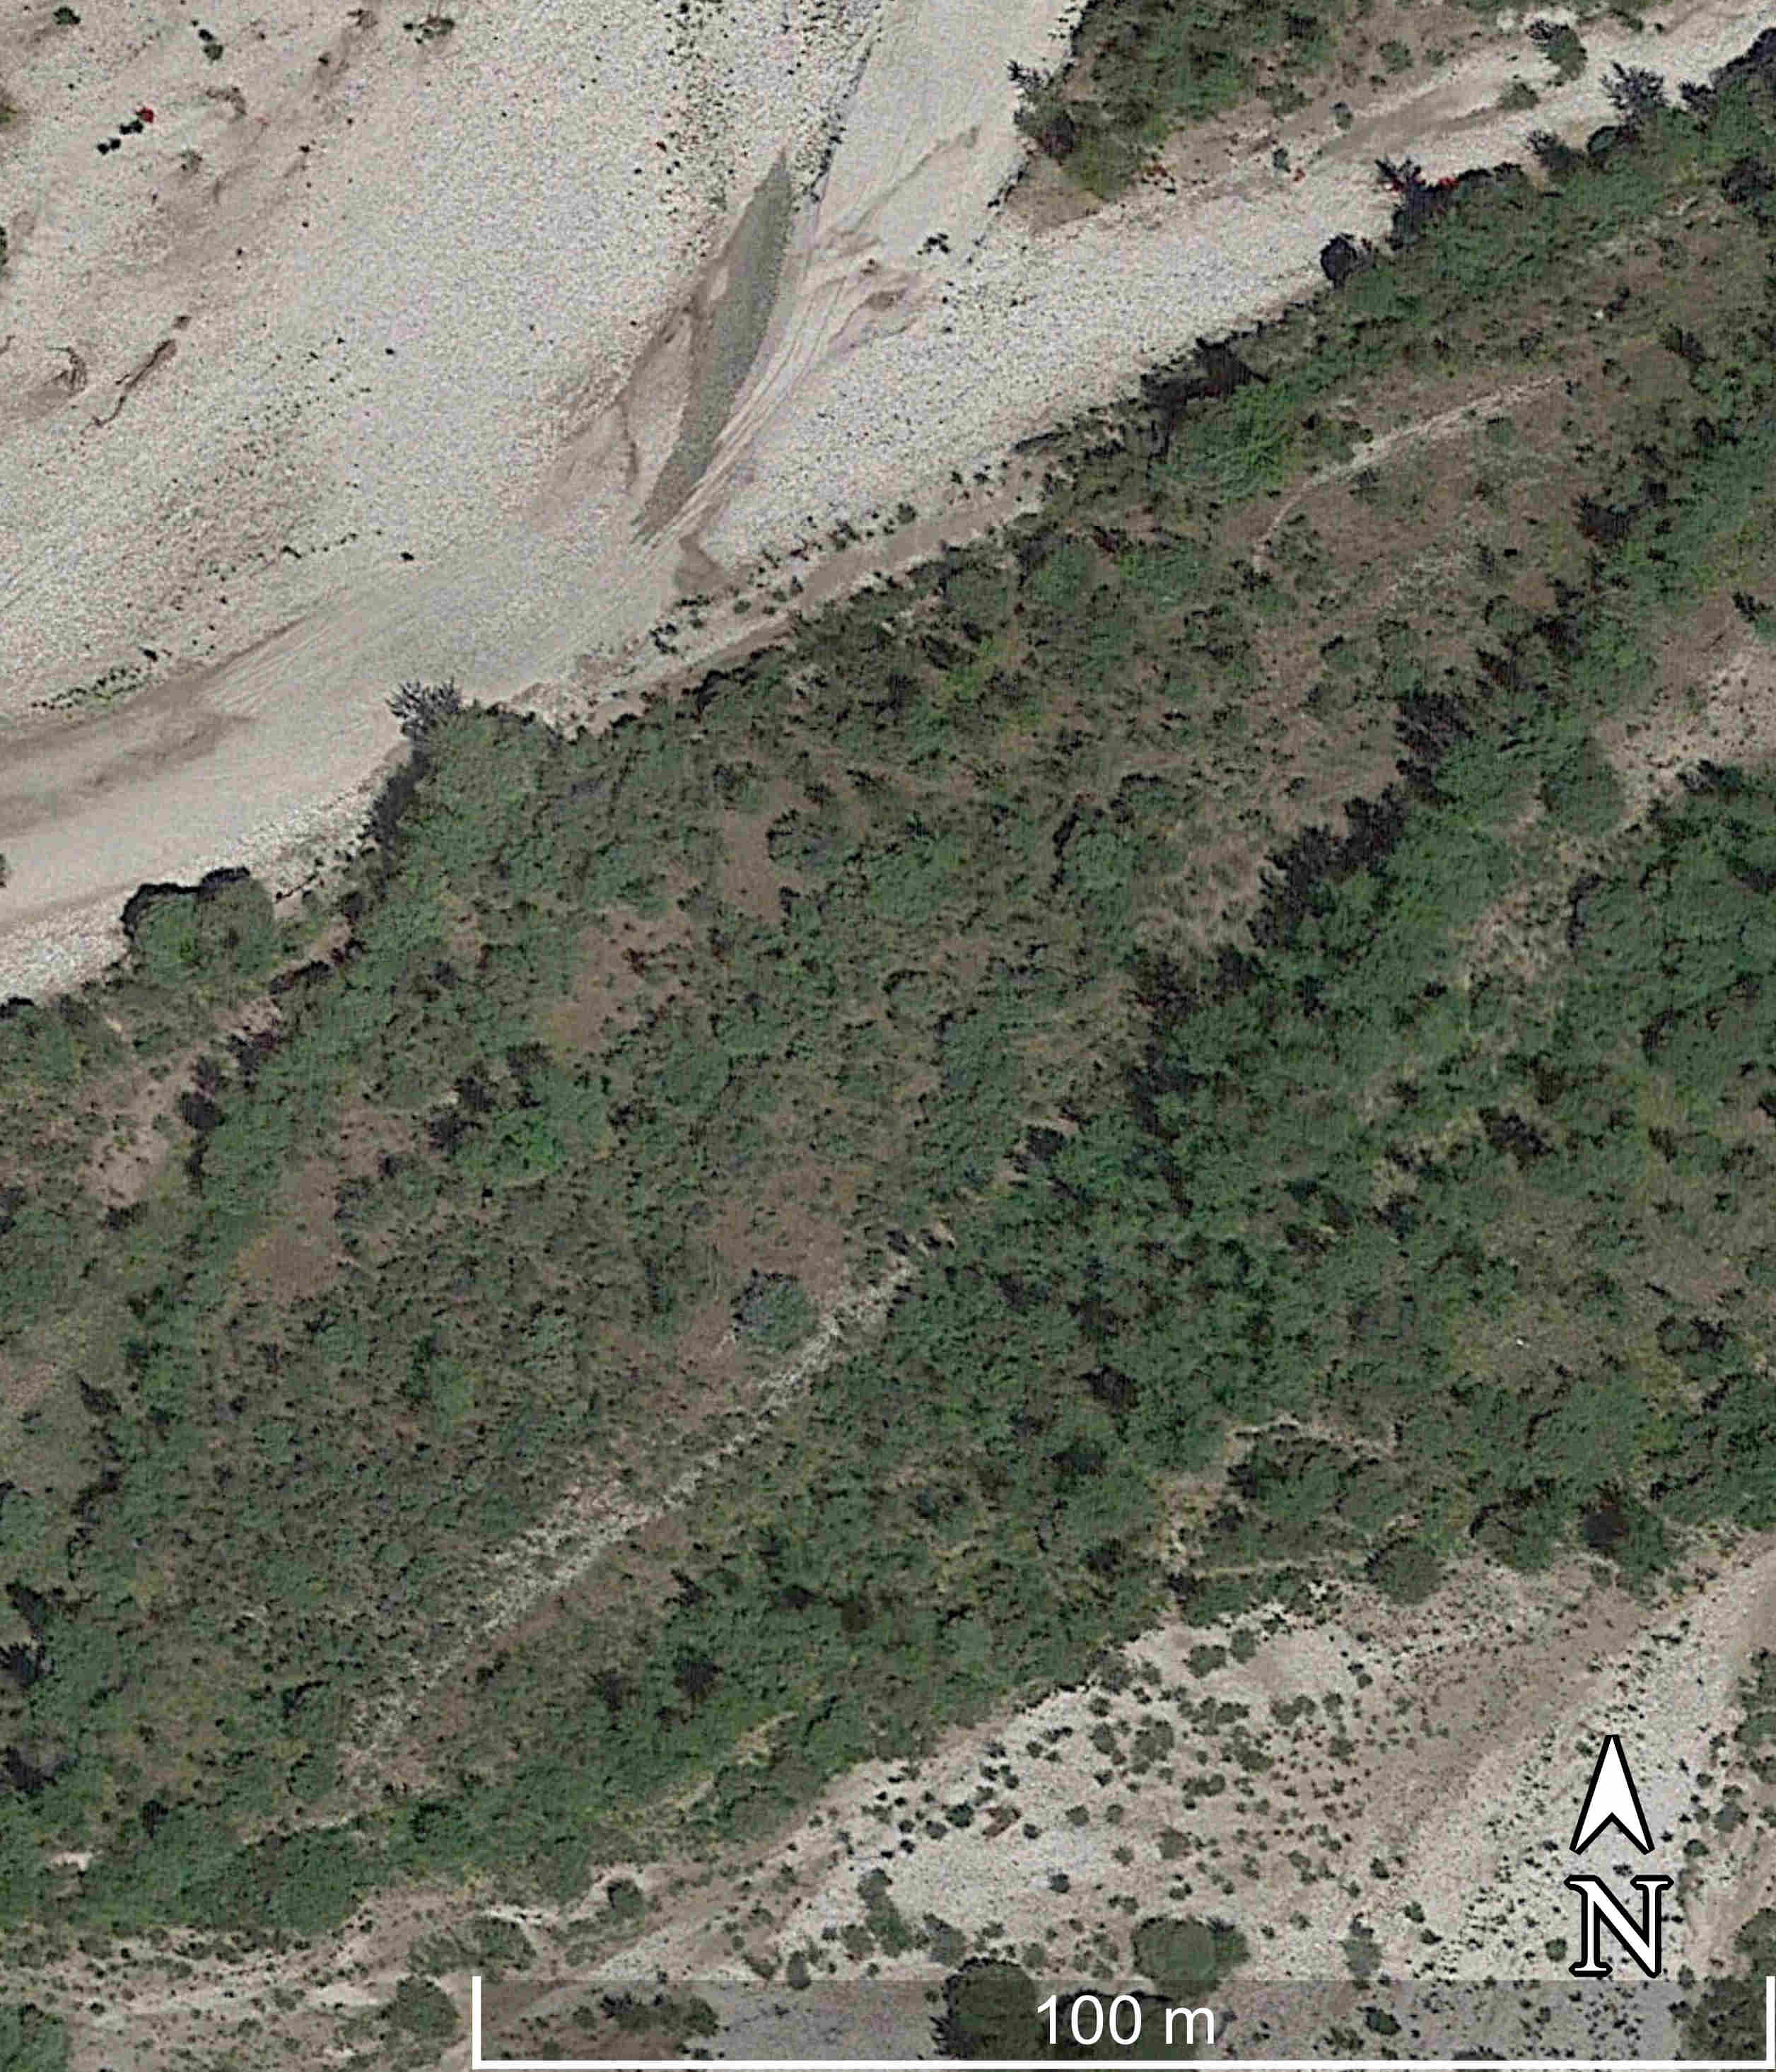
\includegraphics[width=\textwidth]{files/esempio_isola_sat_1.jpg}
	\end{subfigure}
	\quad
	\begin{subfigure}[b]{0.57\textwidth}
		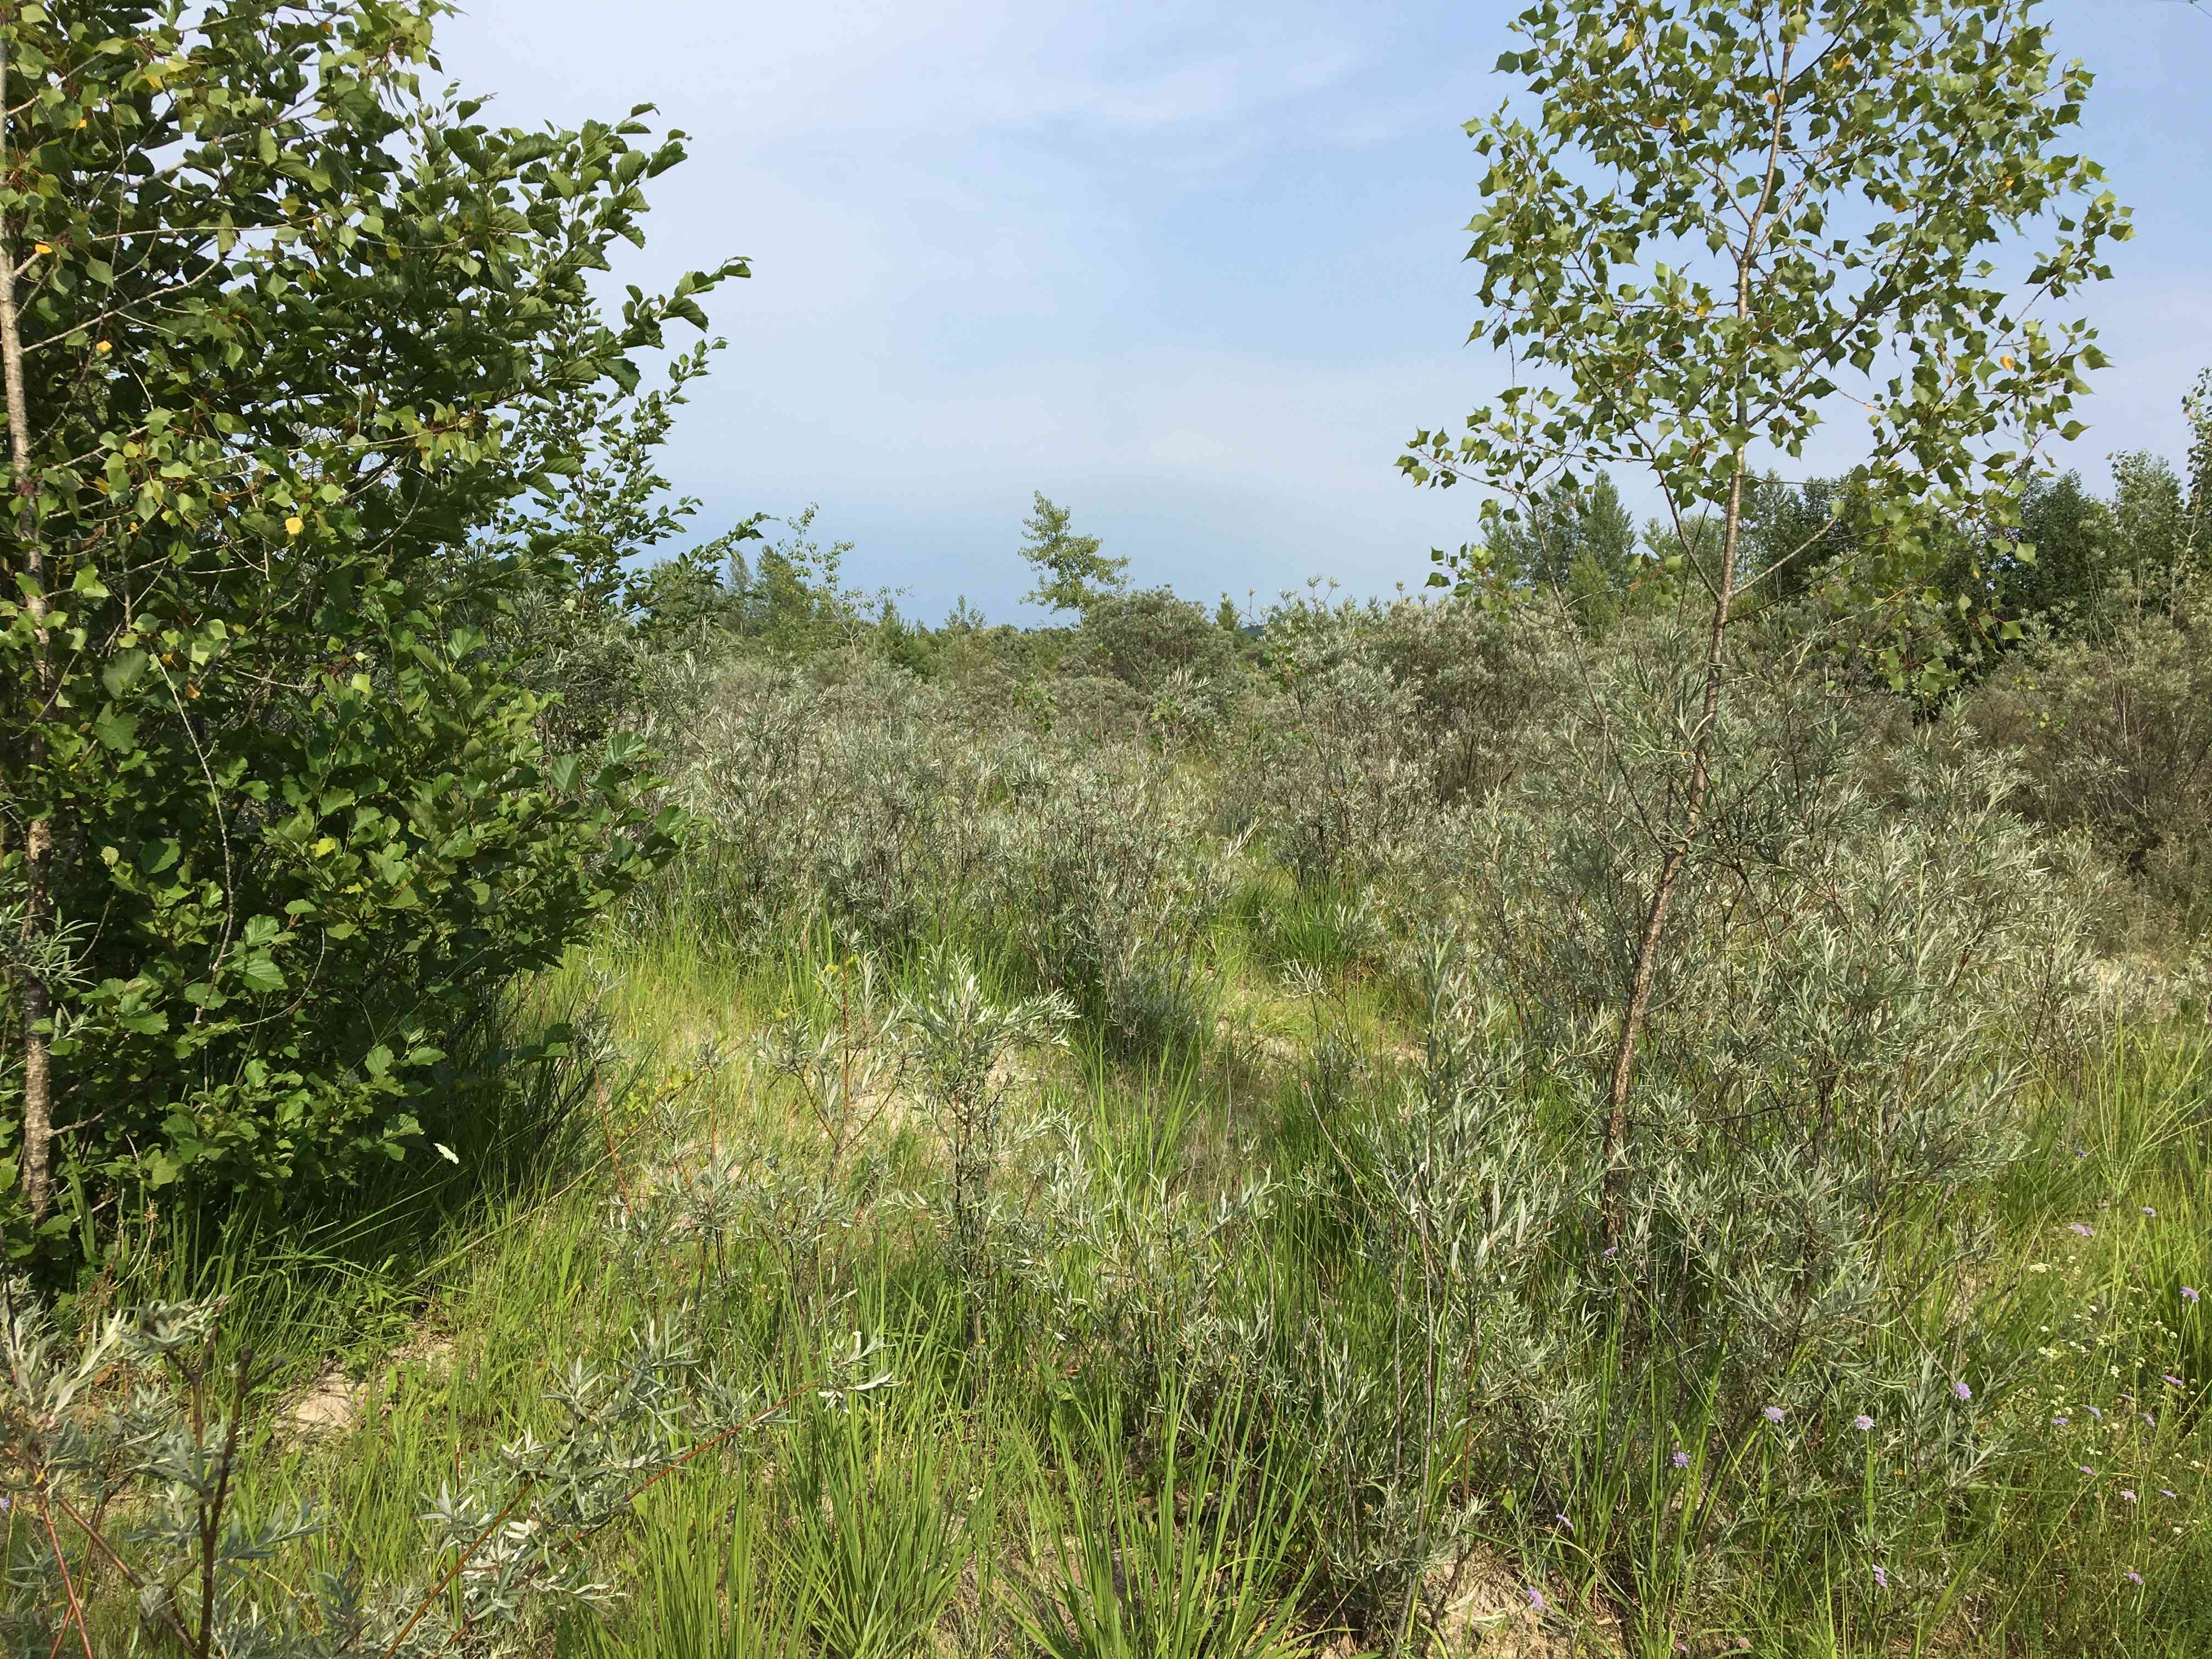
\includegraphics[width=\textwidth]{files/esempio_isola_1.jpg}
	\end{subfigure}
	\caption[immagine e foto di isole fluviali]{immagine da Google Earth e foto di isole fluviali; si noti la forte presenza di salici (\emph{Salix spp.}) e di pioppi (\emph{Populus nigra}); il luogo della foto è prossimo a quello dell'immagine.}
	\label{fig:esempio-isola}
\end{figure}
%
\\
Il meccanismo fondamentale di generazione di forme vegetate in alveo è la ricrescita vegetativa che caratterizza \emph{P. nigra} e \emph{Salix spp.}: i tronchi eradicati e trasportati dalle piene e in seguito depositati sulla nuda ghiaia rigettano rami e foglie (\cref{fig:esempio-accumulo});
se vi è la contemporaneità di adeguate condizioni ambientali (non eccessiva velocità di abbassamento della falda in un substrato di pezzatura adeguata) ed idrologiche (frequenti piene di piccola-media entità, chiamate \emph{flow pulses}) allora i tronchi vivi crescono, intrappolano sedimenti e creano un buon ambiente per la successiva colonizzazione da parte di nuove piante (isole pioniere);
le isole si aggradano (fino a \SI{2}{\m} \squarecite{Gurnell:2006-omega}) e accrescono caratterizzandosi con piante di diversa età (\emph{building island} e isole complesse) \squarecite{Gurnell:2001-island-formation}.
A loro volta la presenza delle isole influenza la posizione, grandezza, forma dei canali e le dinamiche del fondo.
%
\begin{figure}
	\centering
	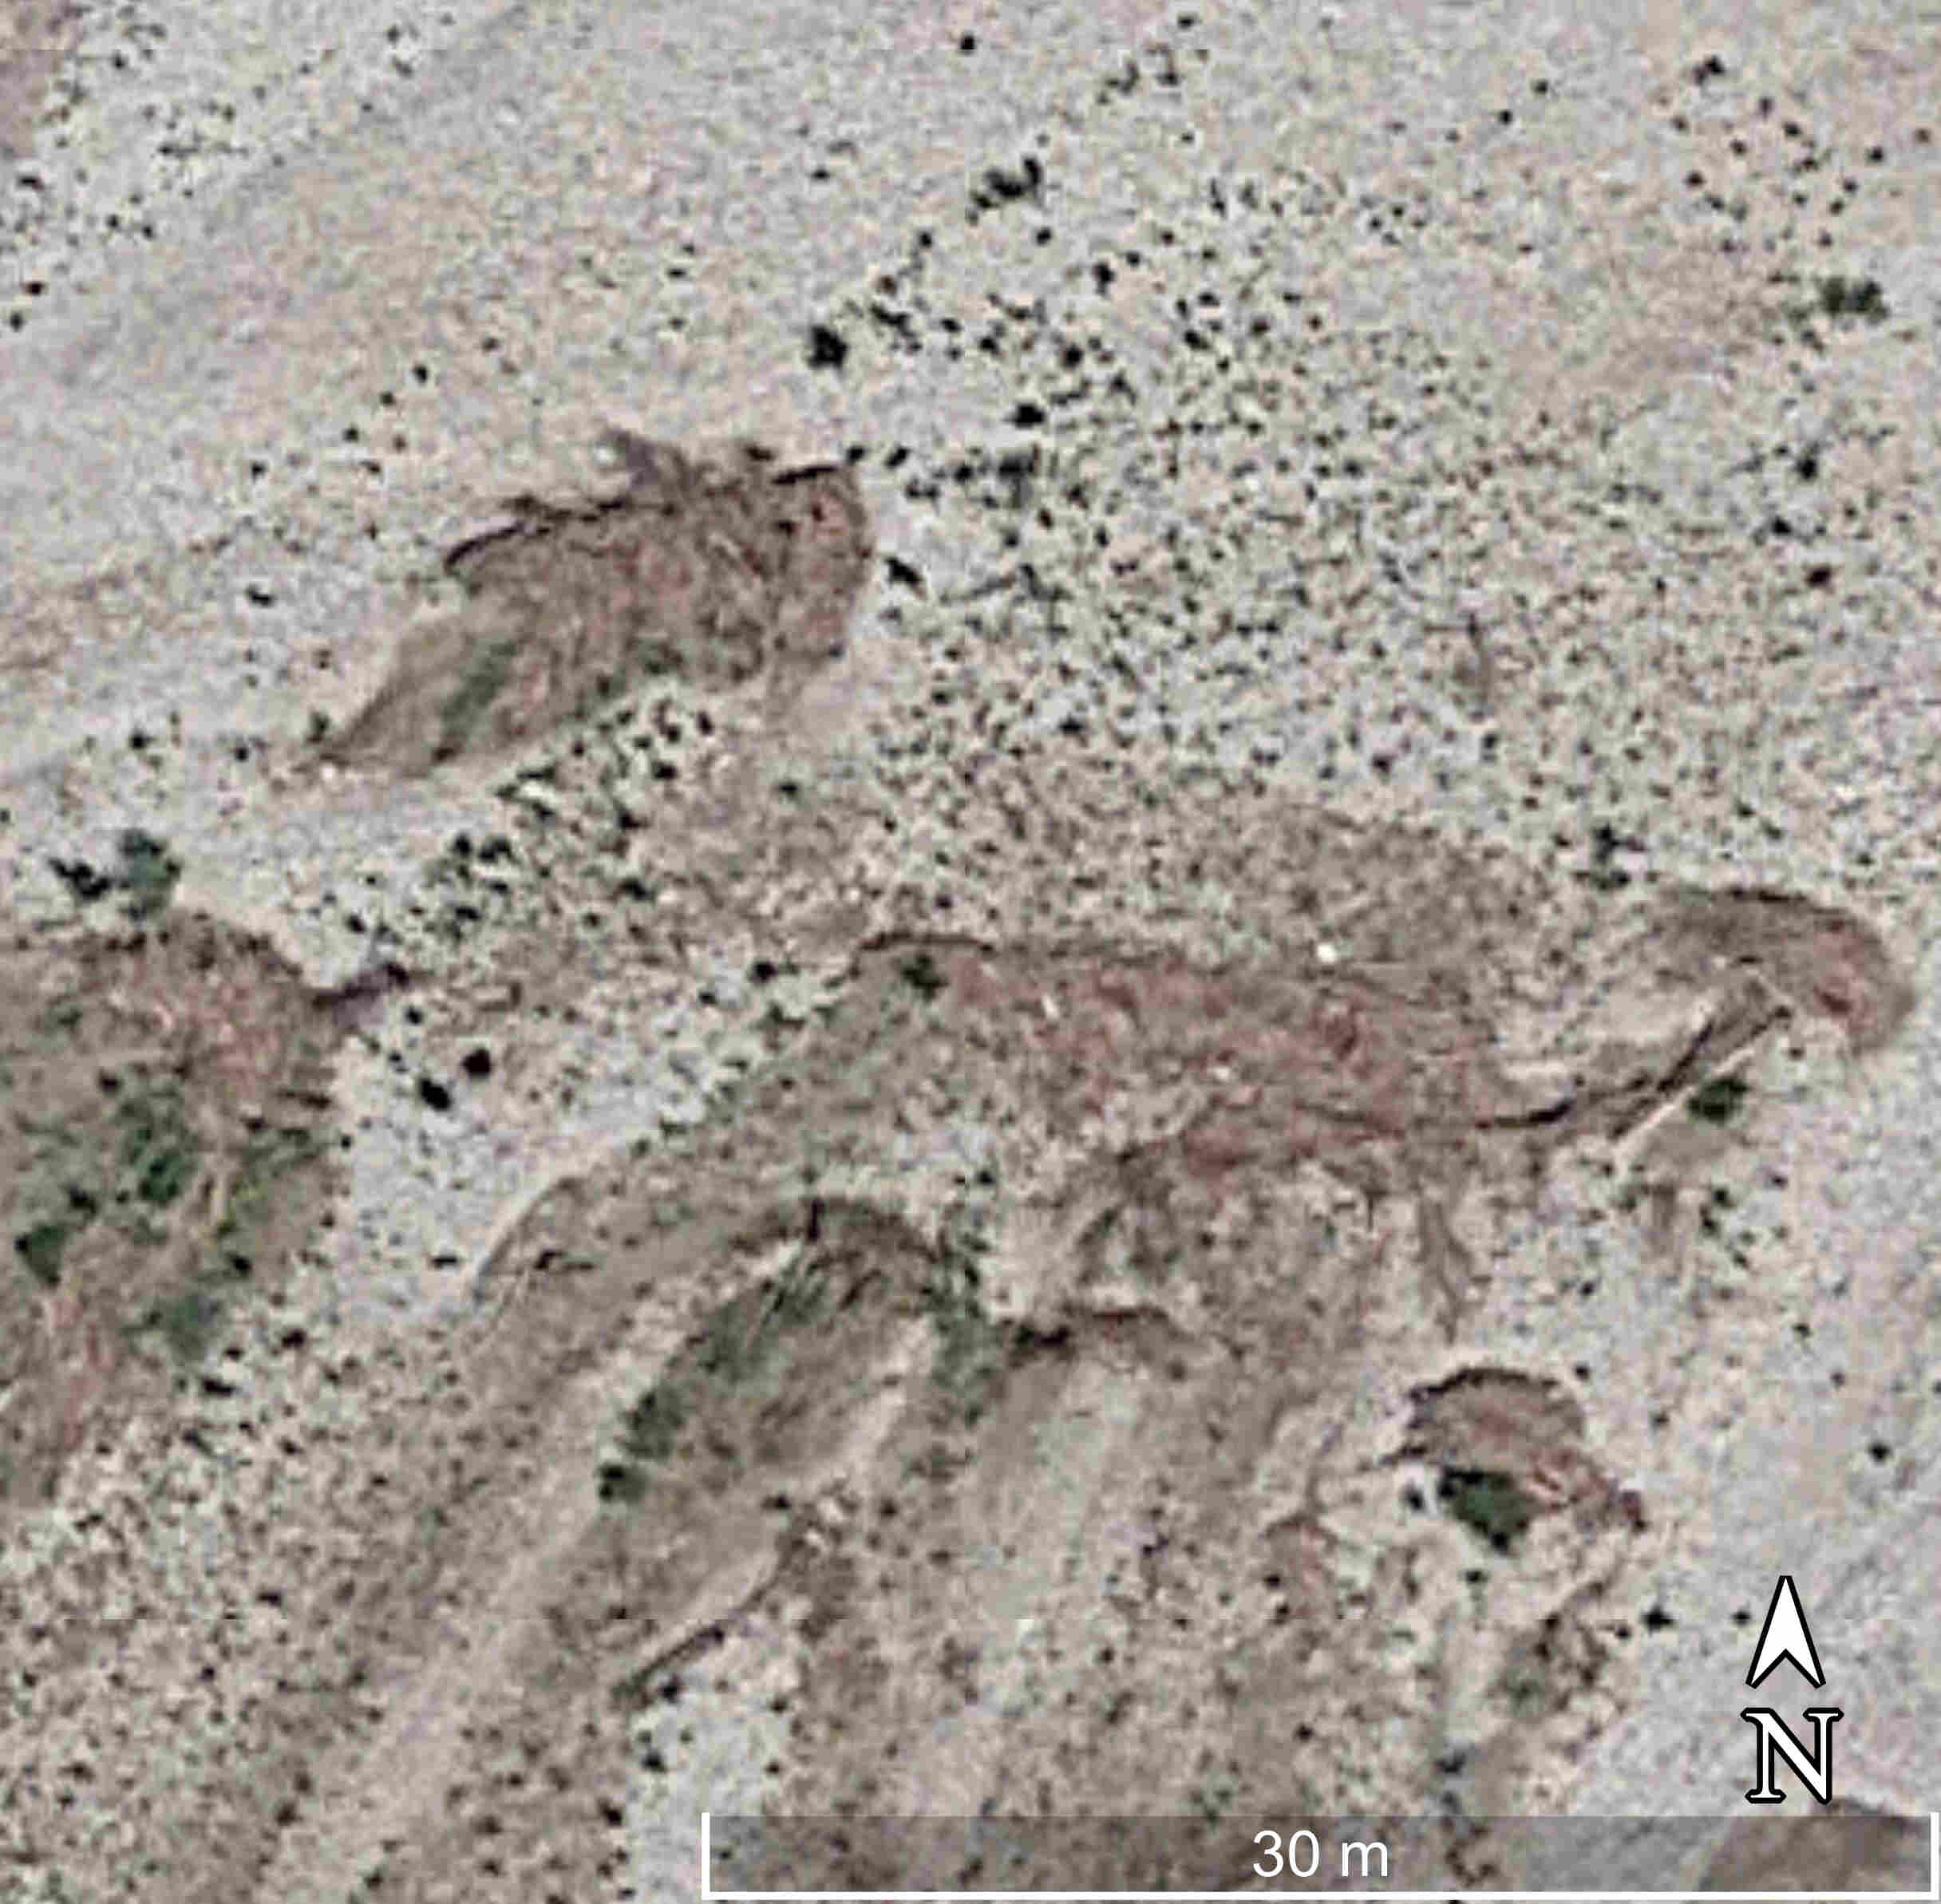
\includegraphics[width = .45\textwidth]{files/esempio_accumulo_sat_1.jpg}
	\quad
	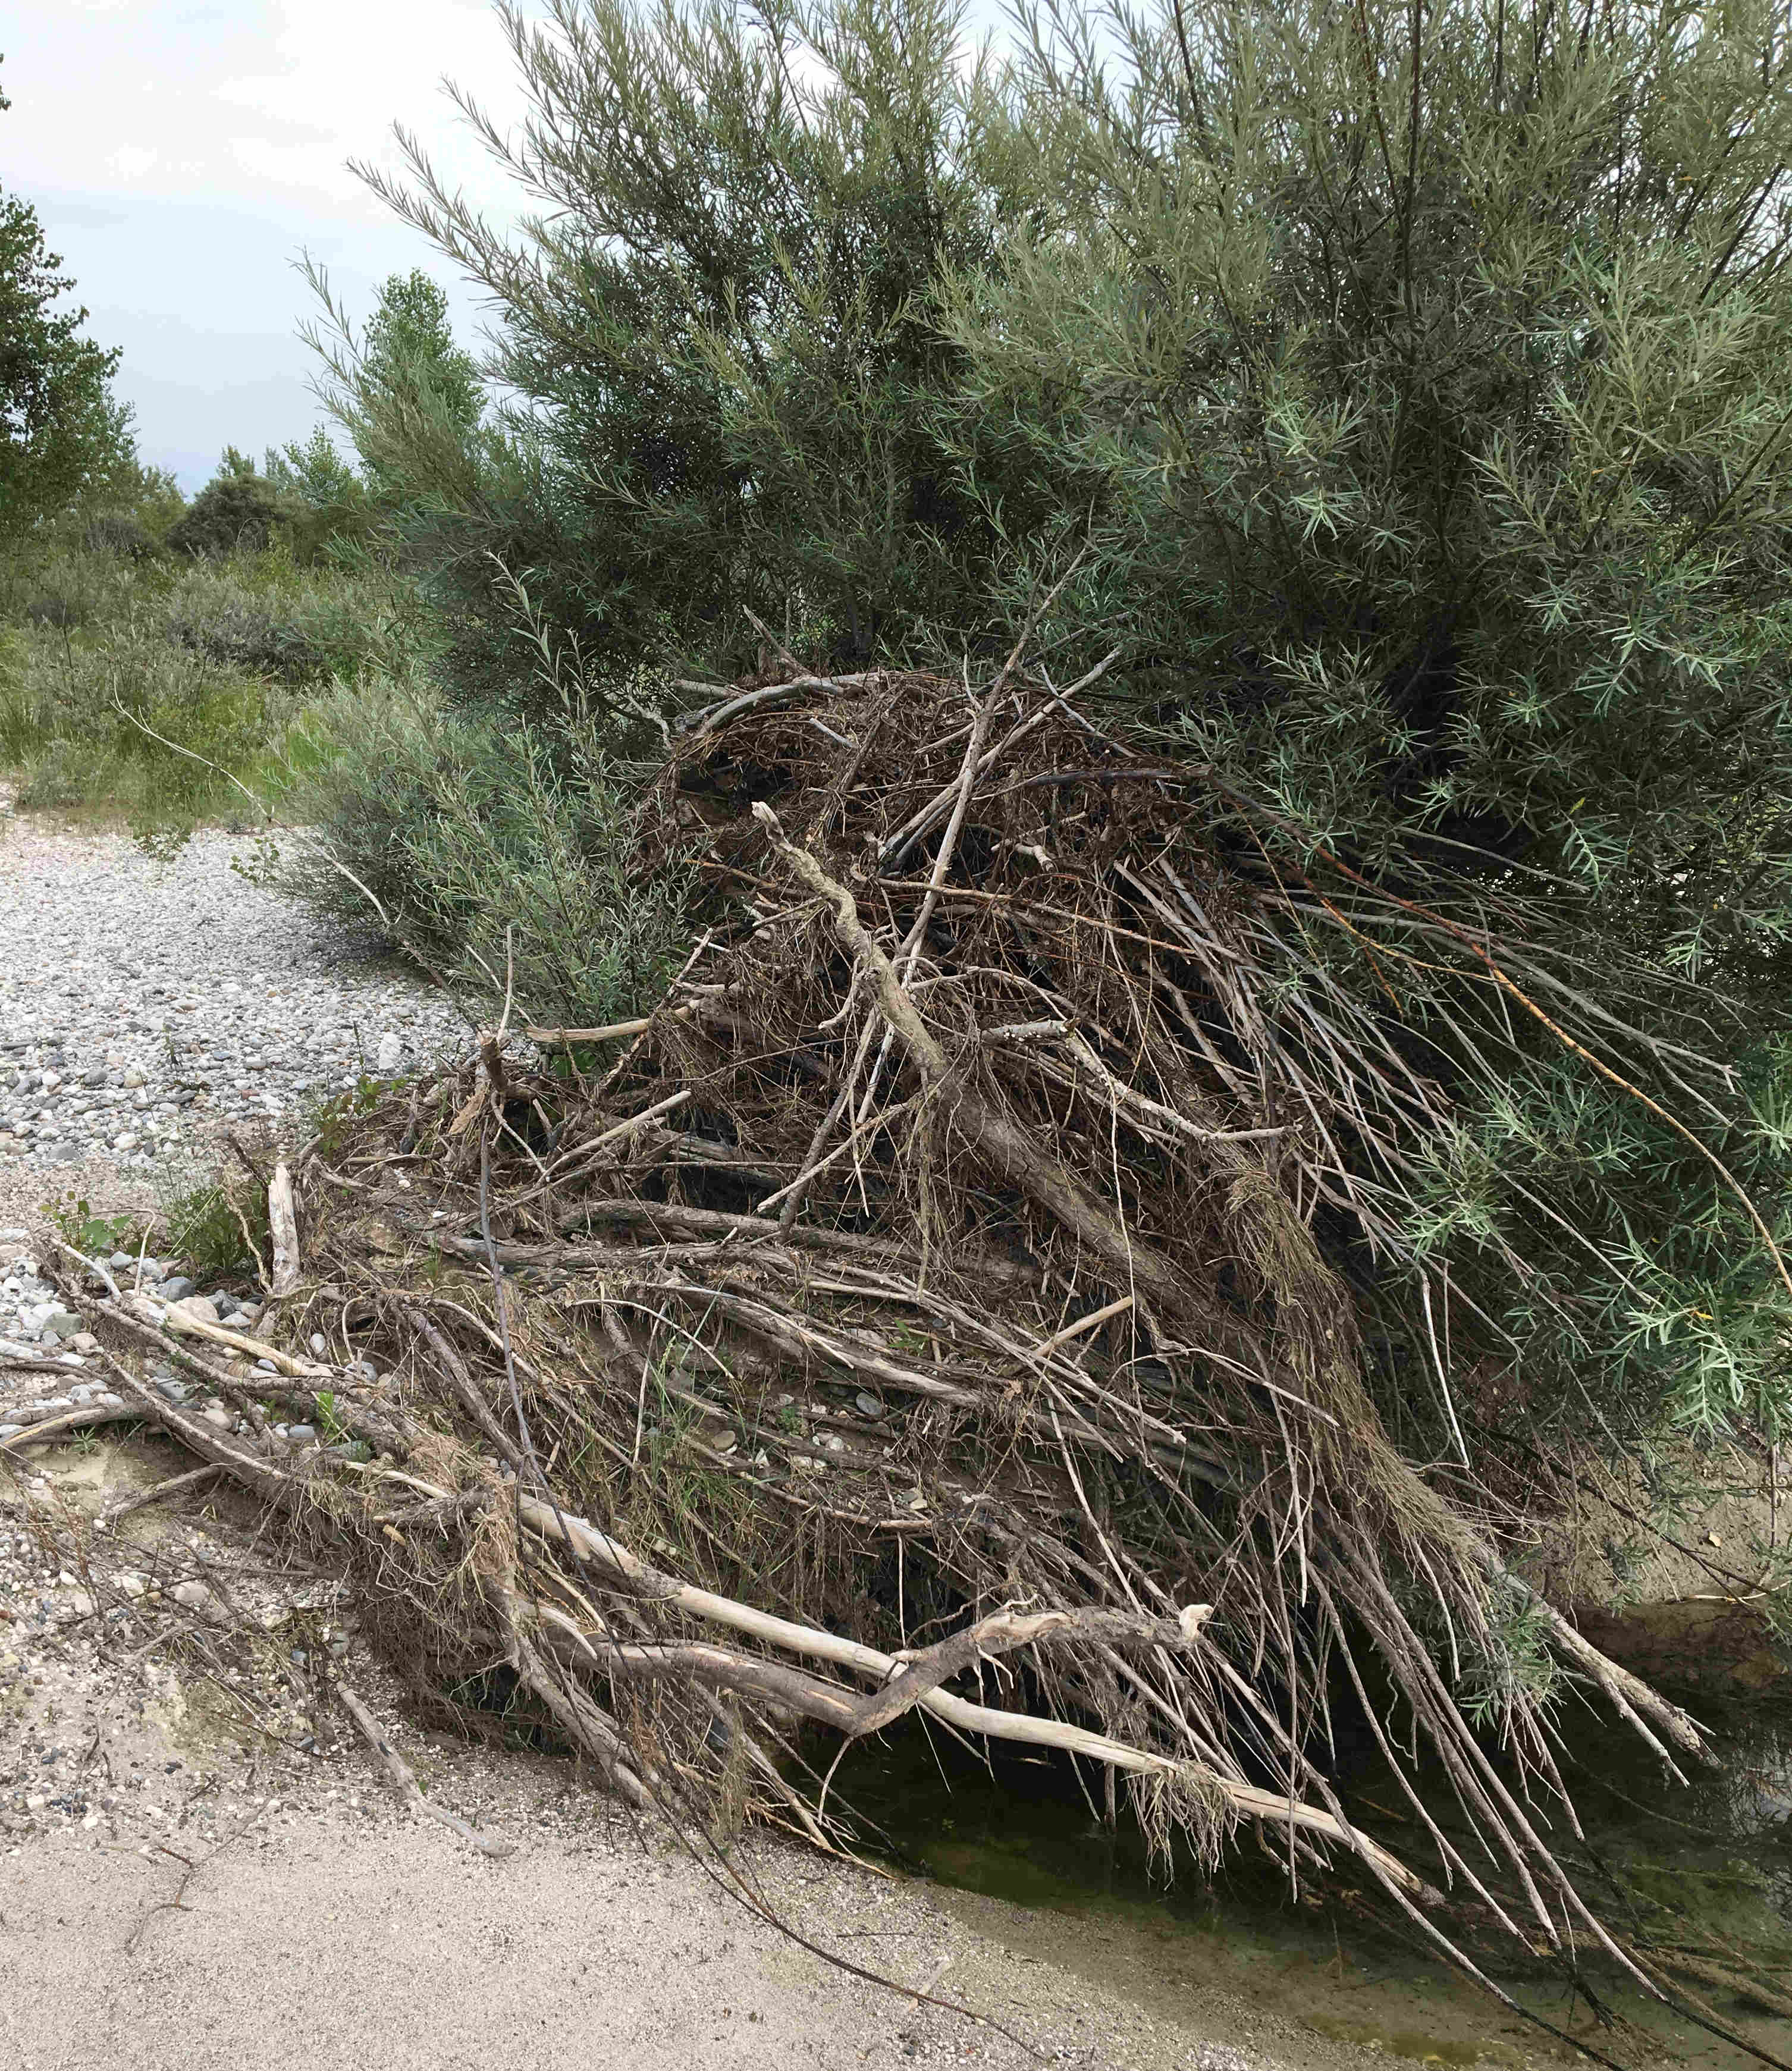
\includegraphics[width = .45\textwidth]{files/esempio_accumulo_1.jpg}
	\caption[immagine e foto di accumuli legnosi]{immagine da Google Earth e foto di accumuli legnosi in grado di rigettare nuovi rami e radici. Il luogo della foto non corrisponde a quello dell'immagine.}
	\label{fig:esempio-accumulo}
\end{figure}
%
\\
Si parla quindi di successione biogeomorfica nel corridoio fluviale attivo: l'ambiente fisico influenza la crescita delle piante coevolute con l'ambiente fluviale; queste a loro volta influenzano l'ambiente fisico e la sua evoluzione, tanto da essere state chiamate “ingegneri ecosistemici” \squarecites{Gurnell:2006-omega}{Gurnell:2014-plants-eng}.

Possono formarsi isole anche da piante nate da seme, anche se queste sono più esigenti in termini di condizioni ambientali ed idrologiche.
\\
Eventi di piena che riempiono l'alveo fino a lambire le sponde (\emph{bankfull}) od eventi più intensi possono dividere parti di vegetazione riparia dalla piana alluvionale, dando origine ad isole composte da piante mature coetanee, strutturalmente ben diverse dalle isole disetanee formate a partire da frammenti vegetativi.

Le isole sono distribuite disomogeneamente da monte verso valle: si può osservare che nei tratti con \emph{upwelling} il loro numero e la velocità di espansione crescono grazie all'acqua che risale dalla falda, mentre nei tratti con \emph{downwelling} la loro presenza diminuisce;
inoltre, nelle zone particolarmente più strette come nei tratti montani o presso la stretta di Pinzano l'intensità della corrente è tale da ridurre o inibire la crescita di vegetazione, come mostrato da un modello concettuale in letteratura \squarecite{Gurnell:2014-plants-eng}.
\\
Temporalmente, le uniche isole che non vengono erose sono quelle che si fondono nella piana alluvionale; anche isole insediatesi da anni in alveo, aggradatesi fino a porsi a quote simili a quelle della \emph{floodplain}, possono essere completamente spazzate durante eventi \emph{bankfull} o maggiori.
Difatti è stato mostrato che la maggior parte delle isole nel tratto compreso tra il ponte autostradale di Braulins e la stretta di Pinzano persistono meno di \SI{24}{\anni} \squarecite{Zanoni:2008}; risultati simili sono stati presentati per un tratto nei pressi di San Paolo~(PN), corrispondente ai tratti più a valle nella presente tesi \squarecite{Bertoldi:2009-2m}.

L'isola presente nel tratto~9 (\cref{fig:23-tratti}), nei pressi di Cornino, si fonda su un nucleo roccioso.
Questa isola non è soggetta alle dinamiche tipiche delle isole che crescono sulla ghiaia dell'alveo: nemmeno le piene più intense possono asportarla od eroderla parzialmente.


\section{Stato dell'arte ed obiettivi}
\label{sec:stato-arte-obiettivi}
L'obiettivo principale della presente tesi è lo studio delle dinamiche delle isole nel Tagliamento in risposta al regime idrologico (successione di magre, morbide, piene) e la comprensione dei fattori che controllano le traiettorie evolutive della vegetazione.
In via previsionale si cerca di rispondere all'esigenza di stimare in anticipo gli effetti che una piena può avere sulle isole, risultato che aiuterebbe anche a migliorare la gestione dei fiumi e della vegetazione presente in essi in altri contesti dove le portate sono regolate dall'uomo. 
\\
Lo studio è stato effettuato su un periodo di 18~anni, dal~2000 al~2018, analizzando dati telerilevati con tecniche diverse (immagini satellitari, foto aeree, rilievi aerei topografici LiDAR).
I dati così ottenuti sono stati messi in relazione al regime idrologico dello stesso periodo, caratterizzato dalle misure idrometriche di livello del pelo libero presso la stazione di Villuzza~(UD). 

Articoli precedentemente pubblicati hanno studiato l'ecologia e la morfodinamica del Tagliamento, le interrelazioni tra piante e fiume, la crescita della vegetazione riparia, la localizzazione delle isole in questo contesto naturale e molto altro.
\\
Alcuni lavori si sono basati su immagini aeree e indagini di campo \squarecites{Zanoni:2008}{Bertoldi:2010-d50}{Surian:2015}: da una parte questi permettono la raccolta di informazioni in grande dettaglio, ma con risoluzione spaziale modesta (i rilievi aerei hanno un costo non indifferente) e risoluzione temporale particolarmente limitata (da pochi anni a decenni tra ogni rilievo).
\\
L'utilizzo di immagini satellitari multitemporali a bassa risoluzione permette di avere una visione d'insieme dei fenomeni, così come di evidenziare differenze spaziali e temporali.
Infatti è già stato dimostrato che è possibile estrarre risultati significativi sulla vegetazione riparia e sulle sue dinamiche da immagini satellitari a bassa risoluzione \squarecites{Bertoldi:2011-ASTER}{Henshaw:2013-LandSat}.
Questi lavori tuttavia hanno utilizzato delle maschere fisse per delimitare l'area attiva, senza distinguere in ogni immagine le isole dalla \emph{floodplain}.
\\
Alcuni autori hanno inoltre formulato modelli concettuali sulle dinamiche vegetazionali nei fiumi, in particolare nel Tagliamento \squarecites{Gurnell:2001-island-formation}{Gurnell:2006-omega}{Gurnell:2014-plants-eng}.
\\
Generalmente, il tratto più frequentemente studiato è quello compreso tra il ponte autostradale di Braulins~(UD) e la stretta di Pinzano.

Con la presente tesi si vuole provare a rispondere alle seguenti domande, anche grazie ai risultati ottenuti in lavori precedenti.
%
\paragraph{Quante isole sono presenti e cosa ne regola la presenza?}
La larghezza media dell'alveo e la percentuale di isole rispetto all'alveo attivo sono state due grandezze studiate per caratterizzare spazialmente e temporalmente il Tagliamento:
%
\begin{itemize}
	\item il tracciamento della traiettoria evolutiva della larghezza ha permesso di vedere come il tratto a monte di Pinzano si sia ristretto negli ultimi due secoli di più del \SI{50}{\percent}, mentre a partire dalla fine del~1900 sembra che l'alveo abbia ripreso un processo di allargamento \squarecites{Zanoni:2008}{Surian:2015};
	gli autori suggeriscono che il restringimento possa essere dovuto alla concomitanza di lievi cambiamenti naturali nel regime delle portate e per l'estrazione di ghiaia dall'alveo per scopi civili negli anni '70 e '80 del secolo scorso, come è avvenuto per altri fiumi simili \squarecite{Sitzia:2016-d50};
	le cause dell'allargamento possono essere il veto all'estrazione della ghiaia congiuntamente ad un periodo caratterizzato da piene intense nei primi anni del 2000;
	%
	%
	\item la proporzione tra isole e alveo attivo è stata considerata da più autori \squarecites{Zanoni:2008}{Bertoldi:2011-ASTER}{Henshaw:2013-LandSat}{Surian:2015}; 
	mentre alcuni risultati sembrano mostrare un rapporto oscillante attorno ad un valore medio di \SI{8}{\percent} \squarecite{Zanoni:2008}, altri mostrano valori abbastanza diversi come ordine di grandezza \squarecite{Henshaw:2013-LandSat} (probabilmente dovuti all'utilizzo di immagini satellitari con celle di \SI{30}{\m}) o con un trend temporale opposto rispetto alla larghezza \squarecite{Surian:2015}.
\end{itemize}	
%
In un modello concettuale presentato pochi anni fa viene proposta la potenza della corrente come fattore che regola la presenza delle isole \squarecite{Gurnell:2006-omega}: se la corrente ha mediamente un'elevata energia per unità di larghezza, allora la crescita delle piante è inibita; se la potenza è inferiore ad una soglia individuata dagli autori, allora la formazione ed espansione delle isole è controllata da altri fattori ambientali, come la quota della falda e la granulometria del substrato dove crescono le piante.

Con i dati di questa tesi è possibile estendere al periodo presente i risultati e le osservazioni effettuate dagli altri autori sulla larghezza e sulla proporzione di isole rispetto all'alveo attivo, così come sfruttare la maggior risoluzione temporale delle immagini per osservare cambiamenti avvenuti in periodi più brevi.
\\
Inoltre, si cerca non solo di verificare l'esistenza di un valore limite della potenza della corrente oltre il quale non crescono più isole, ma di capire se e in che misura questo fattore può influenzare la massima proporzione di isole presenti in alveo.

\paragraph{In quali condizioni e in quale misura cambiano le isole?}
Le isole sono soggette a continue dinamiche di erosione in seguito alle piene e di accrescimento nei periodi tra un evento e quello successivo.
\\
Diversi autori hanno considerato la persistenza media delle isole nell'alveo, dell'ordine di una ventina d'anni; gli stessi hanno quantificato anche la percentuale di isole erose e le nuove aree vegetate \squarecites{Zanoni:2008}{Bertoldi:2009-2m}{Bertoldi:2011-ASTER}{Surian:2015}.
Tuttavia in alcuni lavori la risoluzione temporale è particolarmente bassa (un'immagine ogni decina di anni), in altri il periodo di studio limitato a pochi anni; in tutti il tratto studiato era quello menzionato all'inizio della sezione, lungo circa~\SI{20}{\kilo\m}.
Si può quindi cercare di migliorare ed ampliare questi risultati sia da un punto di vista spaziale che temporale.
\\
La riproduzione vegetativa a partire da tronchi vivi depositati in alveo è uno dei principali meccanismi di formazione delle isole nel Tagliamento \squarecite{Gurnell:2001-island-formation}. 
Grazie alle ortofoto e alle immagini satellitari ad alta risoluzione si può osservare quanto legno è presente in alveo; con i rilievi LiDAR  si può controllare se gli elementi legnosi che non vengono mobilitati dalle piene sono quelli posti a quote relative maggiori; infine, si può cercare quanti tronchi e accumuli legnosi crescono fino a formare nuove isole.

\paragraph{È utile analizzare l'età delle isole?}
Alcuni autori hanno mostrato come la vegetazione riparia delle isole possa avere una diversa struttura di età in base alle modalità di accrescimento e come le piante mature possano essere generalmente più resistenti all'erosione di piante allo stadio iniziale della successione biogeomorfica \squarecites{Gurnell:2001-island-formation}{Gurnell:2014-plants-eng}.
\\
Ad oggi, tuttavia, sembra che nessun autore abbia provato a caratterizzare l'età della vegetazione nelle isole per migliorare risultati riguardo le dinamiche delle isole.
\\
Con questa tesi si prova ad implementare la divisione della vegetazione nelle isole in classi di età e a verificare se e quanto i risultati ne vengono influenzati: sono le piante più giovani quelle che possono essere erose più facilmente?

\paragraph{Qual è la relazione tra regime delle piene e dinamiche delle isole?}
Precedentemente è già stata formulata una relazione tra isole erose e portata \squarecite{Surian:2015};
questa tuttavia è basata su una piccola quantità di dati e non tiene conto dell'invecchiamento della vegetazione tra piene successive, fattore interessante poiché si potrebbe osservare un'erosione differenziata tra isole appena formatesi e isole insediate in alveo da anni.
\\
Riguardo l'accrescimento, al momento attuale non sono noti all'autore lavori che mettano in relazione la crescita della vegetazione con il periodo che intercorre tra piene successive.

\section{Convenzioni}
Le seguenti convenzioni saranno utilizzate nella presente tesi:
\begin{description}
	\item[Capitoli] riprendono le domande formulate nella sezione~\ref{sec:stato-arte-obiettivi}; ogni sezione di risposta è suddivisa in metodi (quali tecniche sono state utilizzate e quali analisi sono state svolte), risultati (cosa è possibile osservare oggettivamente dai dati) e discussione (quale interpretazione è possibile dare ai risultati);
	\item[Mappe] riportate secondo WGS84/UTM~33N (EPSG:~32633);
	\item[Direzione della corrente] riportata con una freccia blu nelle immagini;
	\item[Formato delle date] AAAA-MM-GG;
	\item[Citazioni] sono nel formato Autore/i-Anno, racchiuse tra parentesi quadre;
	\item[Web link] sono riportati in note a piè pagina;
	\item[Termini in lingua straniera] sono in corsivo;
	\item[Glossario] presente nel materiale finale.
	%
\end{description}


%----------------------------------------------------------



\chapter{Materiali e strumenti}
Nel presente capitolo viene inizialmente introdotta l'entità fisica a fondamento di tutto il lavoro: la radiazione elettromegnetica;
in seguito vengono riportati i materiali da cui sono stati estratti i dati per le analisi e gli strumenti utilizzati nelle elaborazioni.


\section{La radiazione elettromagnetica}
Gli strumenti di acquisizione di immagini aeree e satellitari sono sensibili a determinate lunghezze d'onda della radiazione elettromagnetica (\cref{graph:el-mag-radiation}), cioè sono in grado di registrarne solo alcune porzioni (bande).
L'occhio umano può distinguere solo le bande del visibile, mentre i sensori artificiali possono acquisire altre bande della radiazione.
%
\begin{figure}
	\centering
	\tikzsetnextfilename{electromagnetic_radiation}
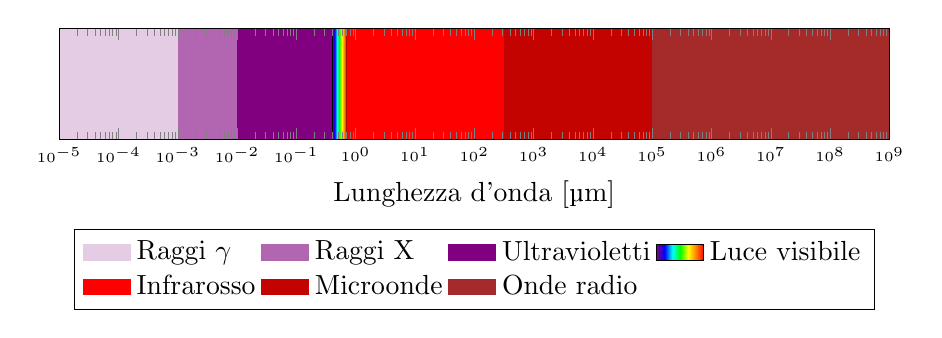
\begin{tikzpicture}[fill between/on layer={axis grid}]
	\begin{axis}[
		xlabel={Lunghezza d'onda},
		xticklabel style = {font=\tiny,yshift=0.2ex},
		xmin=10^-5,
		xmax=10^9,
		x unit=\si{\micro\meter},
		xmode=log,
		ymin=0,
		ymax=1,
		height=3cm,
		width=\textwidth,%12.2cm,
		yticklabels={},
		ytick=\empty,
		legend cell align=left,
		legend style={
			at={(0.5,-0.8)},%(0.85,-0.77)},
			anchor=north,
			legend columns=4,
			}
	]
	\addplot[draw=none, name path=start, forget plot] coordinates{(10^-5,0)(10^-5,1)};
	\addplot[draw=none, name path=gamma, forget plot] coordinates{(10^-3,0)(10^-3,1)};
	\addplot[draw=none, name path=xrays, forget plot] coordinates{(10^-2,0)(10^-2,1)};
	\addplot[draw=none, name path=uv, forget plot] coordinates{(0.4,0)(0.4,1)};
	\addplot[draw=none, name path=visible, forget plot] coordinates{(0.7,0)(0.7,1)};
	\addplot[draw=none, name path=ir, forget plot] coordinates{(10^2.5,0)(10^2.5,1)};
	\addplot[draw=none, name path=microwave, forget plot] coordinates{(10^5,0)(10^5,1)};
	\addplot[draw=none, name path=radiowave, forget plot] coordinates{(10^9,0)(10^9,1)};
	\addplot[violet!20, area legend] fill between[of=start and gamma];
	\addlegendentry{Raggi $\gamma$}
	\addplot[violet!60, area legend] fill between[of=gamma and xrays];
	\addlegendentry{Raggi X}
	\addplot[violet, area legend] fill between[of=xrays and uv];
	\addlegendentry{Ultravioletti}
	\addplot[shading=visiblelight, area legend] fill between[of=uv and visible];
	\addlegendentry{Luce visibile}
	\addplot[red, area legend] fill between[of=visible and ir];
	\addlegendentry{Infrarosso}
	\addplot[Bittersweet, area legend] fill between[of=ir and microwave];
	\addlegendentry{Microonde}
	\addplot[Brown, area legend] fill between[of=microwave and radiowave];
	\addlegendentry{Onde radio}
	\end{axis}
\end{tikzpicture}

	\caption[la radiazione elettromagnetica]{la radiazione elettromagnetica con le sue lunghezze d'onda.}
	\label{graph:el-mag-radiation}
\end{figure}
%
\\
Le immagini nel visibile sono solitamente suddivise nelle bande del Rosso, Verde e Blu (\emph{Red}, \emph{Green}, \emph{Blue}, R-G-B); ognuna indica la quantità di colore presente; la combinazione di queste quantità di colore restituisce l'immagine a colori.
\\
Per poter osservare immagini con bande diverse dal visibile si sostituisce una o più bande R-G-B con le bande in questione.
Ad esempio, è possibile sostituire la banda del Rosso con quella dell'Infrarosso (IR): la quantità di colore del Rosso sarà rimpiazzata dalla quantità di colore dell'Infrarosso.
Il risultato sarà un'immagine riconoscibile dall'occhio umano, ma in falsi colori (\cref{fig:confronto-bande-intro}).
%
\begin{figure}
	\centering
	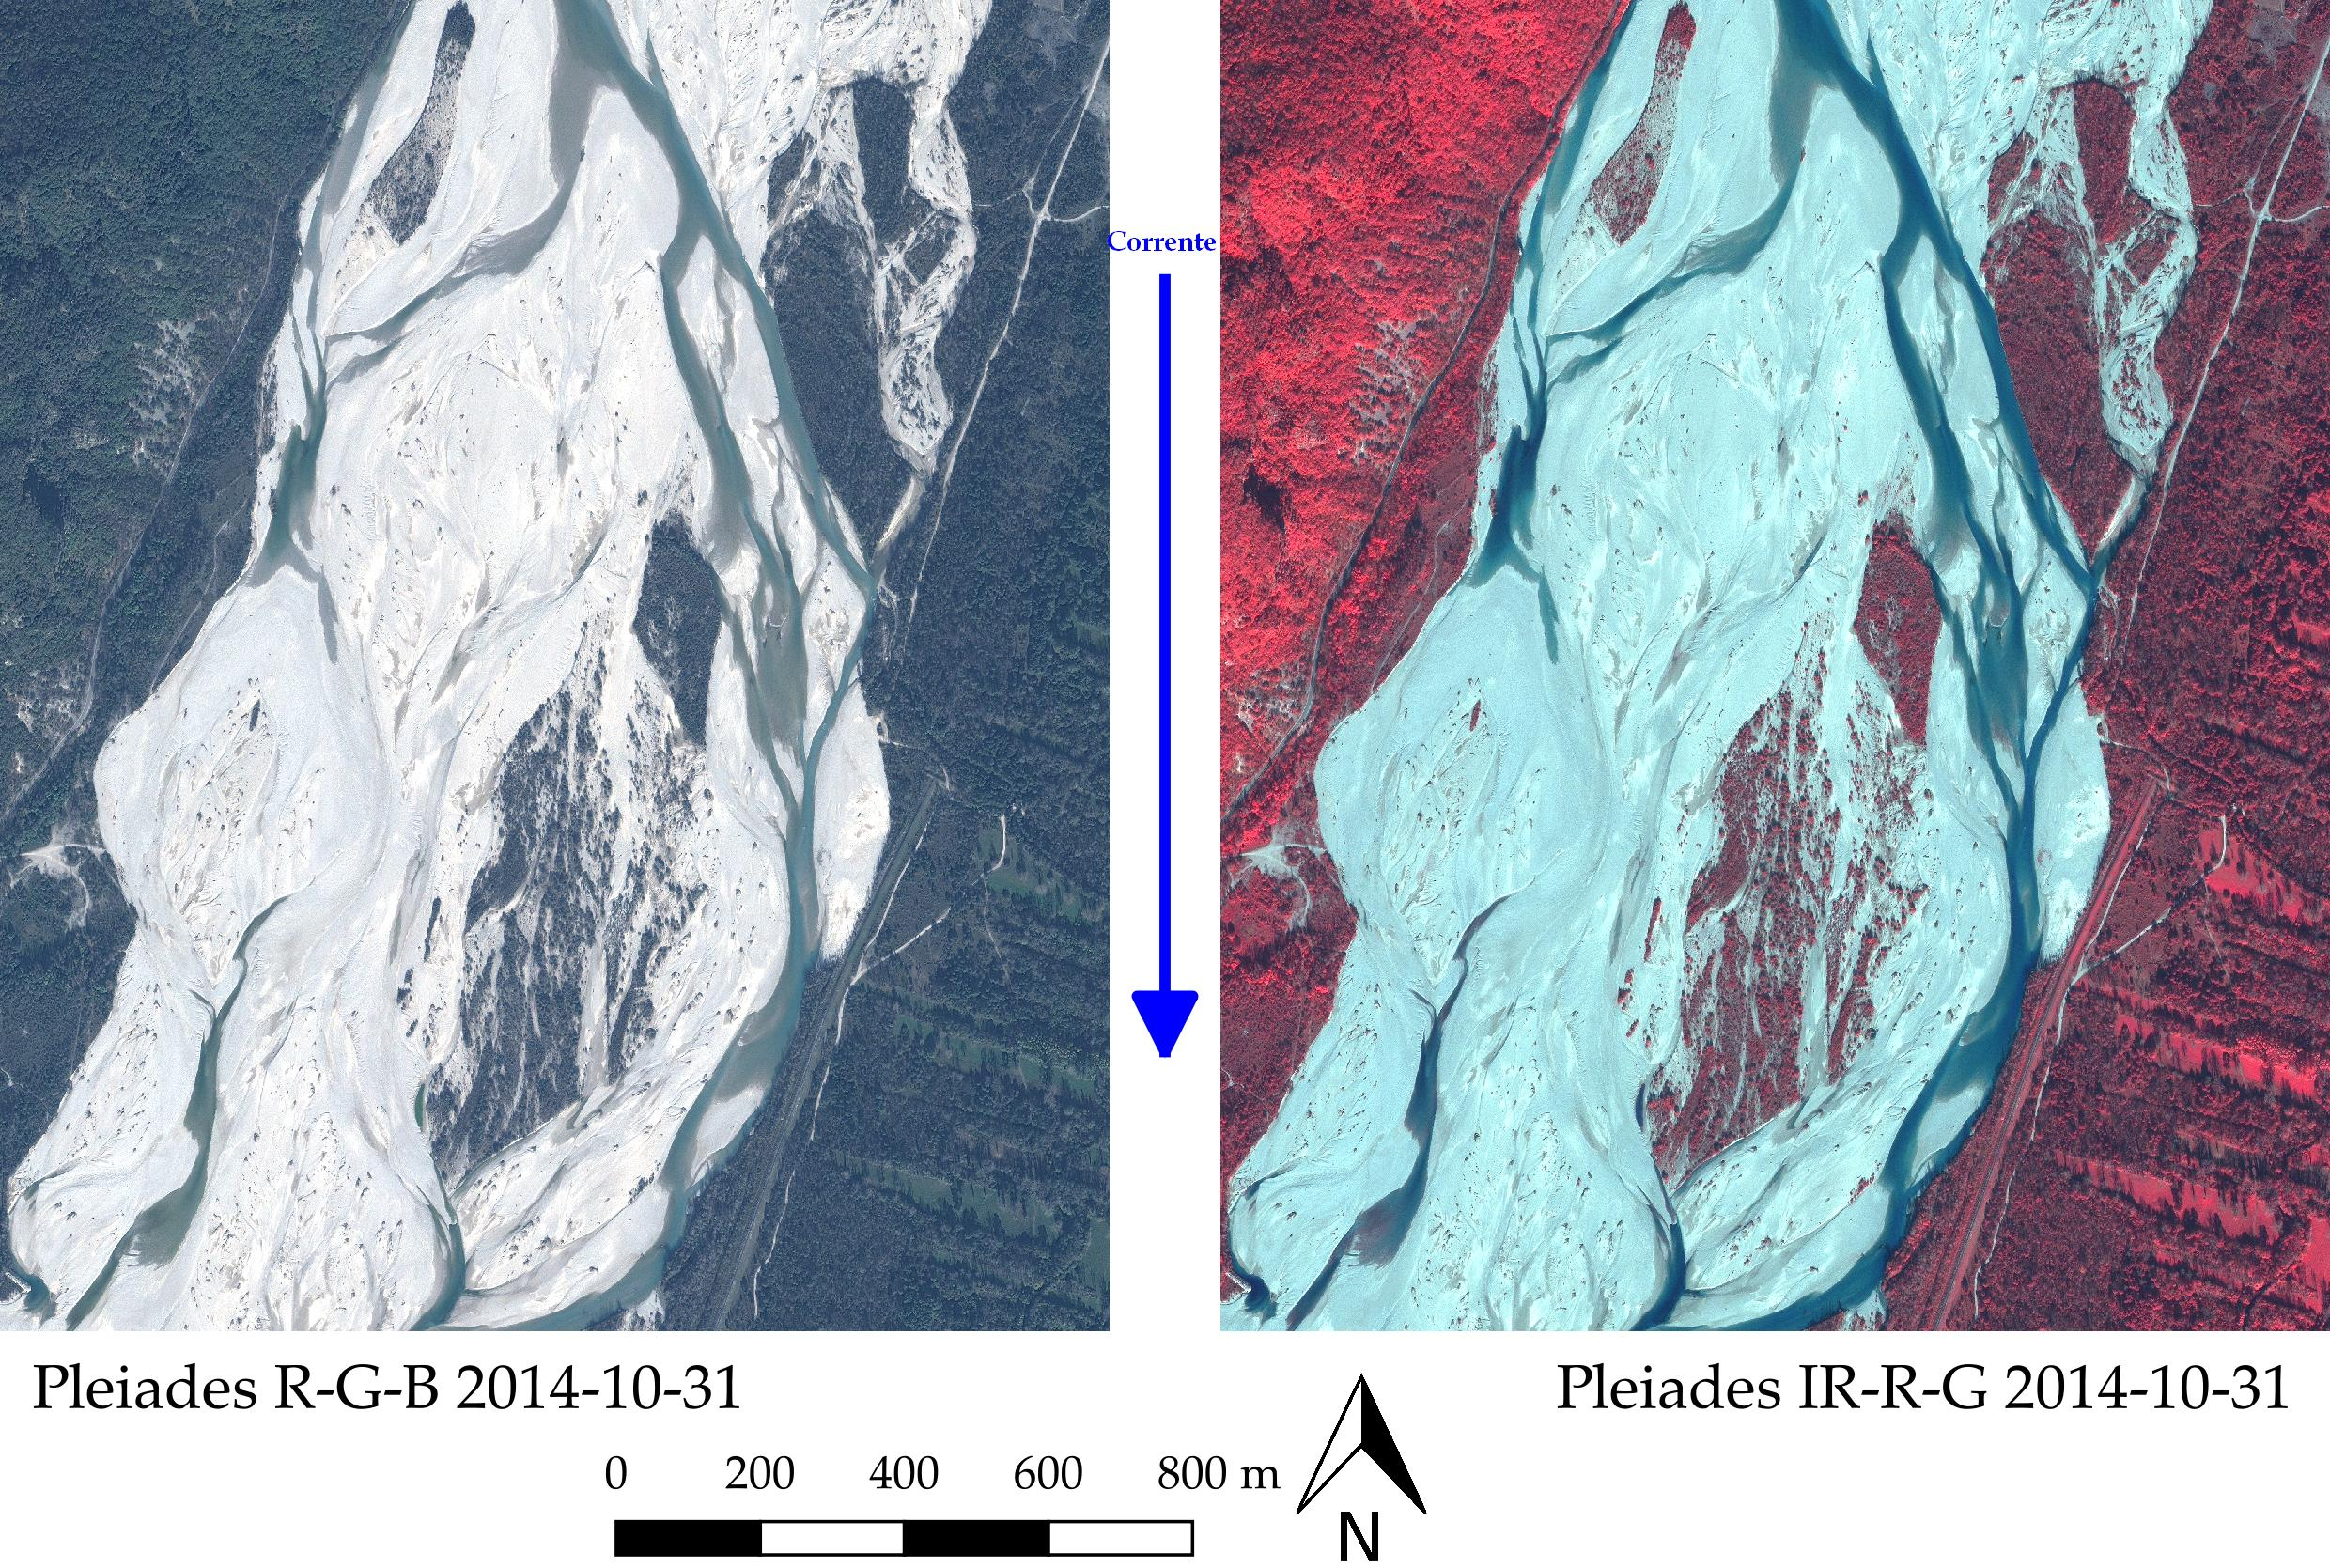
\includegraphics[width=\textwidth]{files/confronto_bande_intro.jpeg}
	\caption[confronto immagini R-G-B e IR-R-G]{confronto di un'immagine in veri colori (R-G-B, a sinistra) con una in falsi colori (IR-R-G, a destra); quest'ultima evidenza la presenza di vegetazione viva rispetto alla ghiaia in alveo e all'acqua nei canali.}
	\label{fig:confronto-bande-intro}
\end{figure}
%
\\
Questo procedimento serve per distinguere più facilmente alcuni elementi e oggetti presenti nelle immagini; per esempio la vegetazione viva riflette particolarmente la banda dell'Infrarosso più vicina al Rosso.



\section{Materiali}
\subsection{Immagini satellitari e rilievi aerei}
Nelle immagini satellitari multibande sia acquisite che di proprietà dell'Università degli Studi di Trento sono state considerate le bande del \emph{Near-InfraRed}~(NIR) e del \emph{Red}~(R), in quanto permettono di distinguere la vegetazione dalle altre coperture del suolo;
le immagini provengono dalle seguenti missioni:
%
\begin{itemize}
	\item satellite Terra, sensore \AST{} Livello~1T (ottenuti in data~21~luglio~2018 e~30~settembre~2018 \squarecite{data:ASTER});  
		\\
		NIR (Banda~3N)~\SIrange[range-phrase={-}]{0.78}{0.86}{\nano\m}, R (Banda~2)~\SIrange[range-phrase={-}]{0.63}{0.69}{\micro\m};
	\item costellazione \Pl{} (\href{https://pleiades.cnes.fr/en/PLEIADES/index.htm}{Centre National d'Etudes Spatiales}\footnote{\texttt{https://pleiades.cnes.fr/en/PLEIADES/index.htm}}), immagini acquistate dall'Università degli Studi di Trento; 
		\\
		NIR~\SIrange[range-phrase={-}]{0.74}{0.94}{\micro\m}, R~\SIrange[range-phrase={-}]{0.59}{0.71}{\micro\m};
	\item satellite \Se{}A-B, sensore~MSI Livello~1C (ottenuti in data 21~luglio 2018 e~21~novembre~2018 tramite il \href{http://scihub.copernicus.eu/}{Copernicus Open Access Hub}\footnote{\texttt{http://scihub.copernicus.eu/}});
		\\
		NIR (Banda~8)~\SIrange[range-phrase={-}]{0.763}{0.908}{\micro\m}, R (Banda~4)~\SIrange[range-phrase={-}]{0.645}{0.683}{\micro\m};
	\item satellite \WV{} (\href{satimagingcorp.s3.amazonaws.com/site/pdf/WV1\_{}WV2\_{}SpectralResponse.pdf}{DigitalGlobe}\footnote{\texttt{satimagingcorp.s3.amazonaws.com/site/pdf/WV1\_{}WV2\_{}SpectralResponse.pdf}}), immagini acquistate dall'Università degli Studi di Trento;
		\\
		NIR (Banda~MS1)~\SIrange[range-phrase={-}]{0.770}{0.895}{\micro\m}, R (Banda~MS2)~\SIrange[range-phrase={-}]{0.630}{0.690}{\micro\m}.
\end{itemize}
%
Le immagini sono state selezionate secondo i seguenti criteri:
%
\begin{itemize}
	\item minima copertura nuvolosa del tratto di studio;
	\item data compresa tra metà aprile e fine ottobre, che è il periodo vegetativo delle piante decidue (\emph{Salix spp.}, \emph{Populus nigra}) che caratterizzano le isole fluviali e la piana alluvionale;
	\item basso livello dell'acqua, per evitare che alcune isole siano sommerse e non visibili;
	\item estensione di almeno qualche decina di chilometri sul tratto di studio.
\end{itemize}
%
Tutte le immagini mostrano la radianza registrata al sensore, sono geometricamente corrette tramite modelli digitali del terreno e georeferenziate secondo la proiezione UTM~33N.

Le ortofoto dell'estate~2011 provengono dal \href{http://www.pcn.minambiente.it/mattm/}{Portale Cartografico Nazionale del Ministero dell'Ambiente e della tutela del territorio e del mare}\footnote{\texttt{http://www.pcn.minambiente.it/mattm/}};
le ortofoto del~2013 sono state ottenute da volo \href{http://www.cgrspa.com/}{CGR}\footnote{\texttt{http://www.cgrspa.com/}} su commissione; 
le ortofoto del~2017 sono state ottenute da \href{https://www.google.com/earth/}{Google Earth}\footnote{\texttt{https://www.google.com/earth/}} (Map data: Google, Digital Globe, European Space Imaging).

Nei mesi di Maggio~2005, Agosto~2010 ed Ottobre~2013 (congiuntamente all'ortofoto) è stato effettuato un rilievo aereo LiDAR, grazie al quale sono a disposizione un DEM (\emph{Digital Elevation Model}) e un CHM (\emph{Canopy Height Model}) per ogni anno: il primo consiste di una mappa con le quote del suolo; il secondo è una mappa di altezza della vegetazione.
Per questi rilievi si ringraziano rispettivamente il UK Natural Environment Research Council, Nicola Surian dell'Università di Padova (progetto CARIPARO) e Yasuhiro Takemon dell'Università di Kyoto.

Il DEM del~2009 proviene dal \href{http://irdat.regione.fvg.it/CTRN/ricerca-cartografia/}{Portale Cartografico della regione autonoma Friuli Venezia Giulia}\footnote{\texttt{http://irdat.regione.fvg.it/CTRN/ricerca-cartografia/}}.

È bene evidenziare che le mappe non hanno tutte la medesima estensione e una piccola parte non comprende tutto il tratto oggetto di studio.
Ciò limita minimamente le analisi che è possibile fare.
\\
Avendo a disposizione 25 immagini per un periodo di studio di quasi \SI{19}{\anni},  si ritiene che la risoluzione temporale sia sufficiente per interpretare i processi che hanno luogo nel Tagliamento: la distanza temporale media tra le mappe è di \SI{274}{\giorni} (circa \SI{0.75}{\anni}), quella minima di \SI{25}{\giorni} e quella massima di \SI{480}{\giorni}.
\\
La risoluzione spaziale varia da~\SIrange[range-phrase={ a }]{15}{0.5}{\m}, adeguata per poter distinguere correttamente le caratteristiche del fiume (limite dell'alveo attivo, isole, canali nella \emph{floodplain}, canali attivi, \ldots).
\\
La \cref{tab:date-orto-sat} mostra le date, la dimensione delle celle delle immagini utilizzate nell'analisi e i tratti validi per ogni immagine.
%%%
\begin{table}[p]
	\centering
	\begin{tabular}{c c S[table-format=2.2] S[range-phrase={$\div$}, list-separator={, }, list-final-separator={, }]}
		\toprule
		Data		&	Tipo		&	\multicolumn{1}{c}{Dim. delle celle \si{[\m]}}	&	\multicolumn{1}{c}{Tratti validi}\\
		\midrule	
		2000-09-17		&	\AST{}		&	15	&	\numrange{1}{21}	\\
		2001-06-07		&	\AST{}		&	15	&	\multicolumn{1}{c}{\numrange[range-phrase={$\div$}]{3}{8}, \numrange[range-phrase={$\div$}]{21}{23}}	\\
		2002-05-18		&	\AST{}		&	15	&	\multicolumn{1}{c}{\numrange[range-phrase={$\div$}]{1}{2}, \numrange[range-phrase={$\div$}]{6}{14}}	\\
		2002-06-12		&	\AST{}		&	15	&	\numrange{14}{23}	\\
		2003-06-22		&	\AST{}		&	15	&	\multicolumn{1}{c}{\numrange[range-phrase={$\div$}]{1}{10}, \numrange[range-phrase={$\div$}]{13}{23}}	\\
		2004-10-14		&	\AST{}		&	15	&	\numrange{2}{23}	\\
		2005-05			&	Rilievo aereo LiDAR	&	2	&	\numrange{6}{14}	\\
		2005-08-30		&	\AST{}		&	15	&	\numrange{1}{23}	\\
		2006-07-16		&	\AST{}		&	15	&	\multicolumn{1}{c}{\numrange[range-phrase={$\div$}]{1}{20}, \numrange[range-phrase={$\div$}]{22}{23}}	\\
		2007-09-21		&	\AST{}		&	15	&	\numrange{1}{23}	\\
		2008-07-05		&	\AST{}		&	15	&	\numrange{1}{23}	\\
		2009			&	DEM			&	20	&	\numrange{1}{23}	\\
		2009-07-08		&	\AST{}		&	15	&	\numrange{3}{23}	\\
		2010-08			&	Rilievo aereo LiDAR	&	1	&	\numlist{7;8;11}	\\
		2010-09-29		&	\AST{}		&	15	&	\numrange{1}{23}	\\
		2011-06-26/07-02	&	Ortofoto	&	1	&	\numrange{6}{12}	\\
		2011-10-02		&	\AST{}		&	15	&	\numrange{1}{23}	\\
		2012-08-01		&	\AST{}		&	15	&	\numrange{1}{23}	\\
		2013-09-05		&	\AST{}		&	15	&	\numrange{1}{23}	\\
		2013-10-22		&	Ortofoto	&	0.2	&	\numlist{7;8;11;12}	\\
		2013-10-22		&	Rilievo aereo LiDAR	&	1	&	\numlist{7;8;11;12}	\\
		2014-09-08		&	\AST{}		&	15	&	\numrange{1}{23}	\\
		2014-10-31		&	\Pl{}	&	0.5	&	\numrange{6}{14}	\\
		2015-08-13		&	\Pl{}	&	0.5	&	\numrange{6}{14}	\\
		2015-09-12		&	\Se{}	&	10	&	\numrange{1}{23}	\\
		2015-10-22		&	\Se{}	&	10	&	\numrange{1}{23}	\\
		2016-09-13		&	\Se{}	&	10	&	\numrange{1}{23}	\\
		2017-04-21		&	\Se{}	&	10	&	\numrange{1}{23}	\\
		2017-06-13		&	\Se{}	&	10	&	\numrange{1}{23}	\\
		2017-06-26/08-02	&	G-Earth	&	0.45	&	\numrange{6}{15}	\\
		2018-06-15		&	\WV{}	&	0.5	&	\numrange{7}{14}	\\
		2018-09-16		&	\Se{}	&	10	&	\numrange{1}{23}	\\
		\bottomrule
	\end{tabular}
	\caption[dettagli delle immagini e rilievi aerei utilizzati]{data e dimensione delle celle delle immagini satellitari, delle ortofoto, del DEM e dei rilievi aerei LiDAR utilizzati.}
	\label{tab:date-orto-sat}
\end{table}


\subsection{Dati idrometrici}
I dati idrometrici orari o semi-orari dal 2000-01-01 al 2018-12-21 presso l'idrometro di Villuzza~(UD) (\SI{46.181}{\degree}N, \SI{12.958}{\degree}E, quota~\SI{240}{\m}~s.l.m.m., corrispondente al ponte di Pinzano) sono stati forniti dalla \href{http://www.protezionecivile.fvg.it/it/rete-idrometeorologica}{rete idrometeorologica della Protezione Civile della Regione Autonoma Friuli Venezia Giulia}\footnote{\texttt{http://www.protezionecivile.fvg.it/it/rete-idrometeorologica}}.
Questi dati riportano l'altezza del pelo libero dell'acqua rispetto ad un livello di riferimento locale dell'idrometro.
La dinamica della morfologia del fondo del fiume non permette di ottenere una scala di deflusso (delle portate) generalmente valida; ciò comunque non costituisce un limite poiché questi dati forniscono adeguate e sufficienti informazioni sulle piene di intensità medio-elevata.
Il grafico in \cref{graph:livelli-matrix} mostra i livelli idrometrici mediati giornalmente; da questi si vede bene come le piene siano generalmente imprevedibili, come abbiano luogo generalmente nei periodi primaverili e autunnali e come si possano alternare anni caratterizzati da pochi eventi con anni che presentano molte piene importanti; si rammenta come proprio questa naturale variabilità del regime delle piene regoli l'abbondanza e la distribuzione delle specie che vivono in ambiente ripario \squarecite{Poff:1997}.
%
\begin{figure}
	\centering
	\tikzsetnextfilename{livelli_matrix}
\begin{tikzpicture}
	\begin{axis}[
		width = \textwidth,
		height = \textwidth,
		enlargelimits = 0,
		ytick distance = 1,
		xtick = {1,31,59,90,120,151,181,212,243,273,304,334,365},
		xticklabels = {{Gennaio}, {Febbraio}, {Marzo},  {Aprile}, {Maggio}, {Giugno}, {Luglio}, {Agosto}, {Settembre}, {Ottobre}, {Novembre}, {Dicembre}},
		xticklabel style = {
			rotate = 90,
		},		
		x tick label as interval,		
		colormap/jet,
		colorbar horizontal,
		colorbar style = {
			xlabel = {Media giornaliera del livello idrometrico},
			x unit = m,
		},	
		]
		\addplot[
			matrix plot*,
			mesh/cols = 365,
			shader = flat corner,
			] % ai dati è stato eliminato il 29 febbraio...! Qualcuno se ne accorgerà mai...?
        	table [x = data, y = anno, point meta = \thisrow{media-gg}] {graphics/data/Dati_Villuzza_matrix.csv};
    \end{axis}
\end{tikzpicture}
	\caption[livelli idrometrici medi giornalieri]{livelli idrometrici medi giornalieri; risulta evidente l'imprevedibilità degli eventi di piena, sebbene questi siano concentrati durante la primavera e l'autunno.}
	\label{graph:livelli-matrix}
\end{figure}

I grafici in \cref{graph:livelli-orto-sat} mostrano rispettivamente i livelli idrometrici e le date di cui si dispongono ortofoto e immagini satellitari (\AST{}, \Pl{}, \Se{}, Google~Earth, \WV{}). 
Nel secondo grafico sono riportati solamente i livelli maggiori di~\SI{1.5}{\m} per mostrare sia le piene di media intensità che quelle più elevate.
Dalla soglia di \SI{2}{\m} si assiste ad una completa connessione di pozze, canali e sorgenti tramite l'inondazione delle barre in ghiaia più alte, iniziando quindi ad esercitare effetti di disturbo sulla vegetazione \squarecite{Bertoldi:2009-2m}.
%
\begin{figure}
	\centering
	\begin{tikzpicture}
	%\begin{groupplot}
	\begin{axis}[
		%name = orto-sat,
		axis y line* = right,
		axis x line* = top,
		%height = .3\textwidth,
		width = \textwidth,
		date coordinates in = x,
		%symbolic y coords = {ASTER,PLEIADES,SENTINEL2,G-EARTH},
		xticklabel = {\year-\month-\day},
		xtick = data,
		ytick = data,
		xticklabel style = {
			rotate = 90,
			anchor = near xticklabel
		},
		enlarge x limits = 0.05,
		enlarge y limits = 0.01,
		ylabel = {Fonte},
		ymax = 3.6,
		ymin = -0.1,
		grid = none,
		only marks,
		]
		\addplot table [x=data, y=numero] {graphics/data/data-orto-sat.txt};
	\end{axis}
	%
	\begin{axis}[
		%name = stages,
		%at = {($(orto-sat.south)-(0,2cm)$)},
		%anchor = north,
		axis y line* = left,
		width = \textwidth,
		date coordinates in = x,
		xticklabel = {\year-\month-\day},
		xticklabel style = {
			rotate = 45,
			anchor = near xticklabel
		},
		enlarge x limits = 0.05,
		enlarge y limits = 0.01,
		ymax = 3.6,
		ymin = -0.1,
		ylabel = {Livello idrometrico},
		grid = major,
		no markers,
		]
		\addplot table [x=data, y=media-gg] {graphics/data/Dati_Villuzza.csv};
	\end{axis}
\end{tikzpicture}
	\tikzsetnextfilename{livelli_2m+imm}
\begin{tikzpicture}
	\begin{axis}[
		width = \textwidth,
		height = 0.5\textwidth,
		date coordinates in = x,
		date ZERO = 2000-01-01,
		xticklabel = {$\year$},
		xticklabel style = {
			rotate = 80,
			anchor = near xticklabel
		},
		xtick distance = 732,
		enlarge x limits = 0.05,
		enlarge y limits = 0.01,
		ymax = 3.7,
		ymin = 1.95,
		ylabel = {Livello idrometrico \si{[\m]}},
		grid = major,
		]
		\addplot+ 
			[red, mark=x, semithick, style=solid, mark=x]
			coordinates {(2000-09-17, 2)(2000-09-17, 3.7)};
		\addplot+ 
			[red, semithick, style=solid, mark=x]
			coordinates {(2001-06-07, 2)(2001-06-07, 3.7)};
		\addplot+
        	[red, semithick, style=solid, mark=x]
        	coordinates {(2002-05-18, 2)(2002-05-18, 3.7)};
		\addplot+
        	[red, semithick, style=solid, mark=x]
        	coordinates {(2002-06-12, 2)(2002-06-12, 3.7)};
		\addplot+
        	[red, semithick, style=solid, mark=x]
        	coordinates {(2003-06-22, 2)(2003-06-22, 3.7)};
		\addplot+
        	[red, semithick, style=solid, mark=x]
        	coordinates {(2004-10-14, 2)(2004-10-14, 3.7)};
		\addplot+
        	[green, semithick, style=solid, mark=x]
        	coordinates {(2005-05-01, 2)(2005-05-01, 3.7)};
		\addplot+
        	[red, semithick, style=solid, mark=x]
        	coordinates {(2005-08-30, 2)(2005-08-30, 3.7)};
		\addplot+
        	[red, semithick, style=solid, mark=x]
        	coordinates {(2006-07-16, 2)(2006-07-16, 3.7)};
		\addplot+
        	[red, semithick, style=solid, mark=x]
        	coordinates {(2007-09-21, 2)(2007-09-21, 3.7)};
		\addplot+
        	[red, semithick, style=solid, mark=x]
        	coordinates {(2008-07-05, 2)(2008-07-05, 3.7)};
		\addplot+
        	[red, semithick, style=solid, mark=x]
        	coordinates {(2009-07-08, 2)(2009-07-08, 3.7)};
		\addplot+
        	[green, semithick, style=solid, mark=x]
        	coordinates {(2010-08-01, 2)(2010-08-01, 3.7)};
		\addplot+
        	[red, semithick, style=solid, mark=x]
        	coordinates {(2010-09-29, 2)(2010-09-29, 3.7)};
		\addplot+
        	[green, semithick, style=solid, mark=x]
        	coordinates {(2011-07-01, 2)(2011-07-01, 3.7)};
		\addplot+
        	[red, semithick, style=solid, mark=x]
        	coordinates {(2012-08-01, 2)(2012-08-01, 3.7)};
		\addplot+
        	[red, semithick, style=solid, mark=x]
        	coordinates {(2013-09-05, 2)(2013-09-05, 3.7)};
		\addplot+
        	[green, semithick, style=solid, mark=x]
        	coordinates {(2013-10-22, 2)(2013-10-22, 3.7)};
		\addplot+
        	[red, semithick, style=solid, mark=x]
        	coordinates {(2014-09-08, 2)(2014-09-08, 3.7)};
		\addplot+
        	[black, semithick, style=solid, mark=x]
        	coordinates {(2014-10-31, 2)(2014-10-31, 3.7)};
       	\addplot+
        	[black, semithick, style=solid, mark=x]
        	coordinates {(2015-08-13, 2)(2015-08-13, 3.7)};
		\addplot+
        	[cyan, semithick, style=solid, mark=x]
        	coordinates {(2015-09-12, 2)(2015-09-12, 3.7)};
		\addplot+
        	[cyan, semithick, style=solid, mark=x]
        	coordinates {(2015-10-22, 2)(2015-10-22, 3.7)};
		\addplot+
        	[cyan, semithick, style=solid, mark=x]
        	coordinates {(2016-09-13, 2)(2016-09-13, 3.7)};
		\addplot+
        	[cyan, semithick, style=solid, mark=x]
        	coordinates {(2017-04-21, 2)(2017-04-21, 3.7)};
		\addplot+
        	[cyan, semithick, style=solid, mark=x]
        	coordinates {(2017-06-13, 2)(2017-06-13, 3.7)};
		\addplot+
        	[green, semithick, style=solid, mark=x]
        	coordinates {(2017-07-07, 2)(2017-07-07, 3.7)};
       	\addplot+
        	[violet, semithick, style=solid, mark=x]
        	coordinates {(2018-06-15, 2)(2018-06-15, 3.7)};
		\addplot+
        	[cyan, semithick, style=solid, mark=x]
        	coordinates {(2018-09-16, 2)(2018-09-16, 3.7)};
		\addplot+
        	[blue, solid, no markers]
        	table [x=data, y=media-gg] {graphics/data/Dati_Villuzza.csv};
	\end{axis}
\end{tikzpicture}
	\caption[livelli idrometrici e foto aeree - satellitari]{in alto il livello idrometrico (in blu) presso l'idrometro di Villuzza, registrato con frequenza oraria o semi-oraria. 
	In basso un ingrandimento per i livelli medi giornalieri superiori a~\SI{1.5}{\m}, che sono indice di piene con effetti non trascurabili.
	I simboli indicano le immagini satellitari e le ortofoto considerate (\AST{} in rosso, ortofoto, rilievi aerei LiDAR e G-Earth in verde, \Pl{} in nero, \Se{} in azzurro, \WV{} in viola).}
	\label{graph:livelli-orto-sat}
\end{figure}



\section{Strumenti}
Per eseguire le analisi sulle immagini aeree e satellitari sono stati utilizzati i GIS GRASS \squarecite{soft:GRASS} e QGIS \squarecite{soft:QGIS}. 
\\
Per l'estrazione delle immagini satellitari \AST{} dagli archivi \texttt{.hdf} è stato usato SCP, plugin di QGIS \squarecite{soft:SCP}. 
\\
Per il download delle ortofoto dell'estate~2017 si è utilizzato \href{https://github.com/sourcepole/qgis-openlayers-plugin}{OpenLayers}\footnote{\texttt{https://github.com/sourcepole/qgis-openlayers-plugin}}, plugin di QGIS.
\\
Per le analisi dei dati sono stati realizzati script in Python~2.7.5 utilizzando la libreria PyGRASS\footnote{\texttt{https://grass.osgeo.org/programming7/}} \squarecite{Zambelli:2013-pygrass} e in Python~3.7.1\footnote{\texttt{https://www.python.org}}.

%----------------------------------------------------------



\chapter{Quante isole sono presenti?}
\section{Metodi: caratterizzare l'alveo}
Si è quantificato l'areale delle isole presenti in alveo avendo accortezza di distinguerlo chiaramente dall'areale della \emph{floodplain}, il quale è soggetto a dinamiche diverse rispetto alle isole.
\\
Per classificare il terreno occupato dall'alveo è stato seguito l'approccio di altri autori in analisi simili eseguite su immagini \AST{} e LandSat~TM \squarecites{Bertoldi:2011-ASTER}{Henshaw:2013-LandSat}.
\\
Sono stati ottenuti in seguito la larghezza media dell'alveo e la potenza della corrente di ogni tratto.

\subsection{Classificazione dell'alveo}
\paragraph{Maschera computazionale}
Dapprima è stata individuata manualmente una maschera di calcolo che comprendesse l'alveo attivo e la parte di piana alluvionale che è stata erosa quando coinvolta nelle piene; 
tale maschera si estende da Tolmezzo al ponte di Madrisio
(\cref{fig:esempio-maschera}). 
Applicandola, il dominio computazionale è stato ridotto, in modo tale da comprendere l'inviluppo degli alvei attivi che si sono succeduti dall'immagine del~2000 a quella del~2018.
%
\begin{figure}[t]
	\centering
	\begin{subfigure}[b]{0.4\textwidth}
		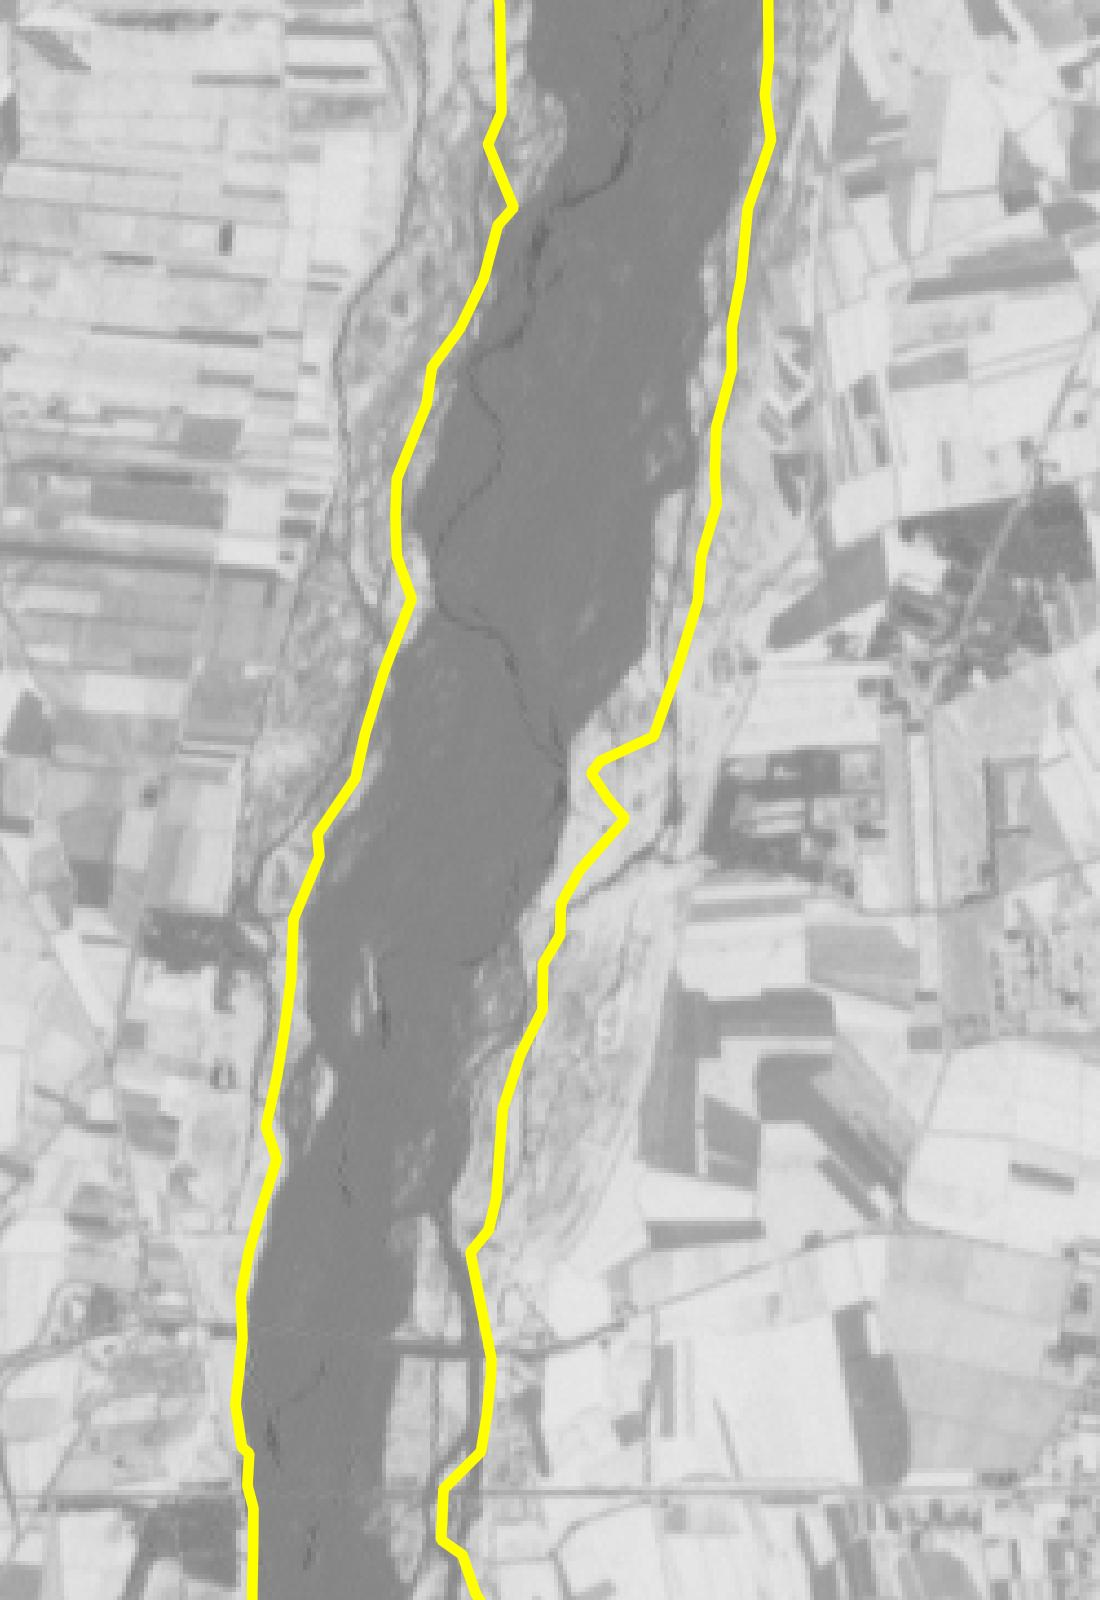
\includegraphics[width=\textwidth]{files/esempio_mask_2002_06_12.jpeg}
		\caption{\AST{} 2002-06-12.}
	\end{subfigure}
	\qquad
	\begin{subfigure}[b]{0.4\textwidth}
		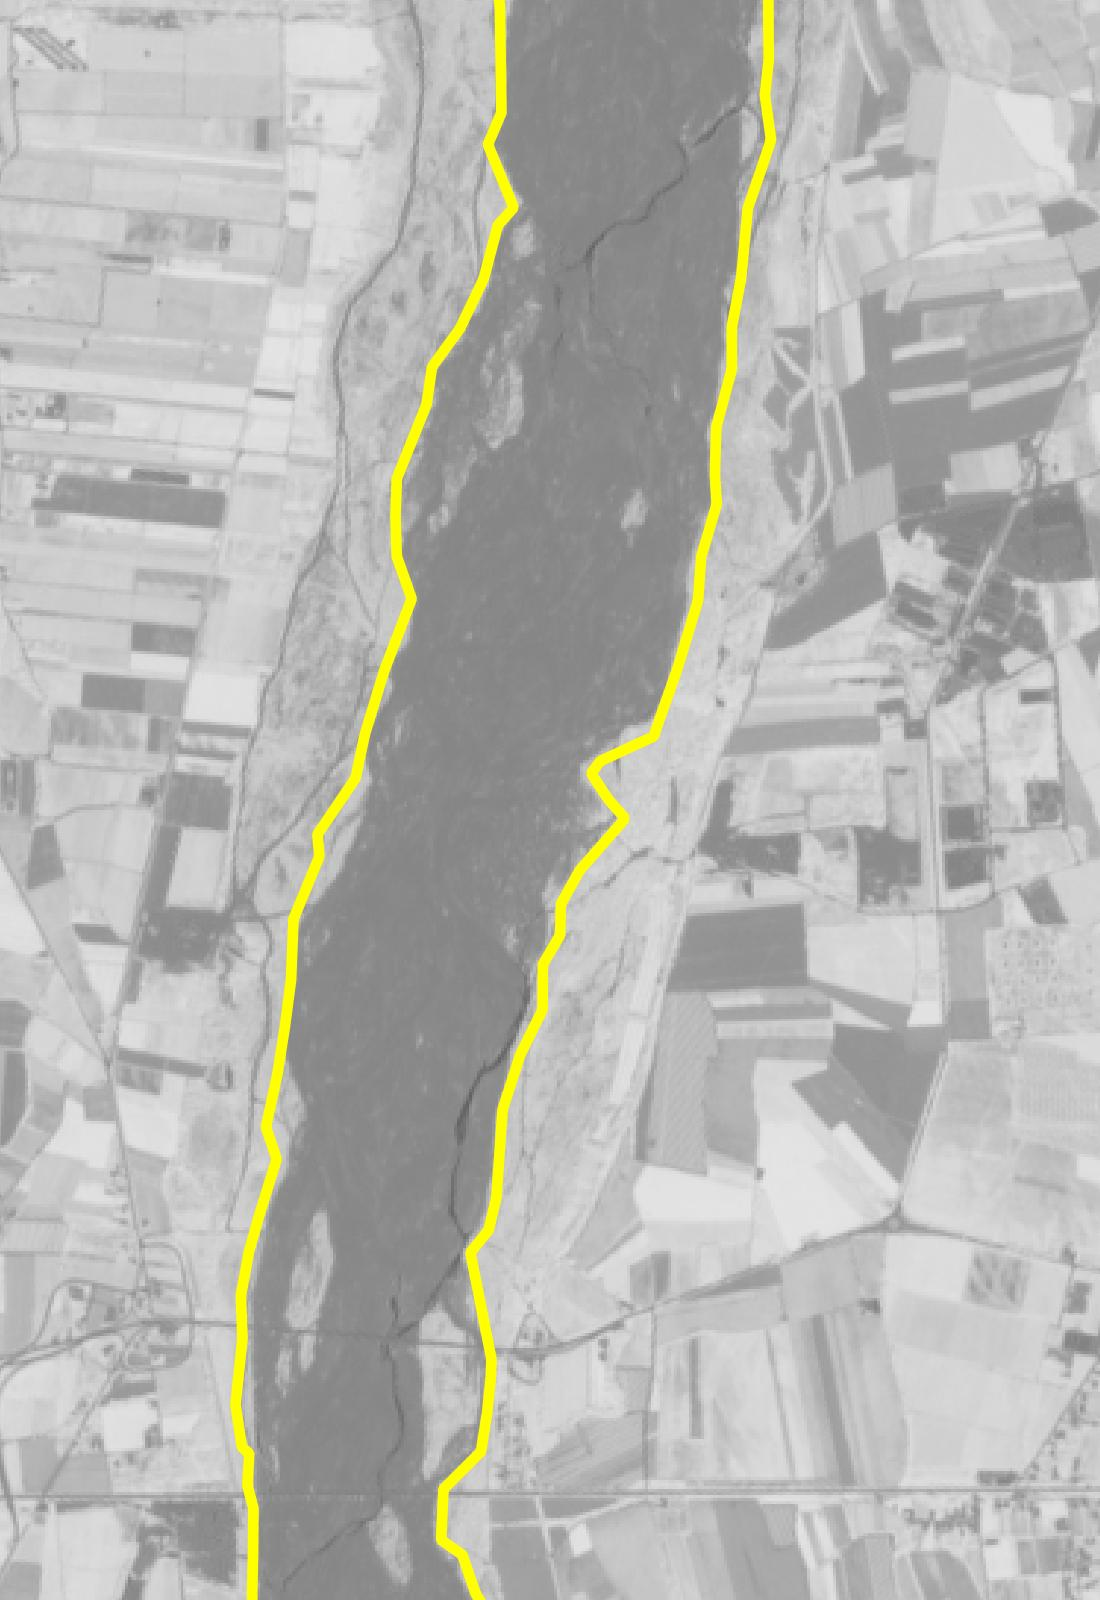
\includegraphics[width=\textwidth]{files/esempio_mask_2015_09_12.jpeg}
		\caption{\Se{} 2015-09-12.}
	\end{subfigure}
	\caption[definizione della maschera per limitare il dominio computazionale]
		{esempio in cui si vede come la maschera utilizzata per limitare il dominio computazionale (in giallo) sia il risultato dell'inviluppo degli alvei attivi che si sono modificati nel tempo; le immagini sono le mappe di NDVI.}
	\label{fig:esempio-maschera}
\end{figure}
%
%
\paragraph{NDVI} 
In questa area è stato calcolato il \emph{Normalized Difference Vegetation Index} (NDVI) grazie alle bande del \emph{Near Infrared} (NIR) e del \emph{Red} (R)
%
\begin{equation}
	%\notag
	NDVI = \frac{NIR - R}{NIR + R} \quad .
	\label{eq:ndvi}
\end{equation}
%
%
\paragraph{Aree campione}
\`{E} stata effettuata una digitalizzazione manuale di alcune aree campione per le immagini \AST{} del~2005-08-30 (\num{\sim 70}) e del~2012-08-01 (\num{\sim 100}), le immagini \Pl{} del~2014-10-31 (\num{\sim 40}) e del~2015-06-13 (\num{\sim 40}), l'immagine \Se{} del~2017-04-21 (\num{\sim 45}) e l'immagine \WV{} del 2018-06-15 (\num{\sim 55}) (\cref{fig:esempio-aree-campione}).
	Sono state selezionate immagini per ogni satellite poiché ciascuno è sensibile a bande leggermente diverse. 
	\\
	Queste aree campione sono state suddivise in tre classi: vegetazione, alveo attivo e canale.
	%
	\begin{figure}[ht]
		\centering
		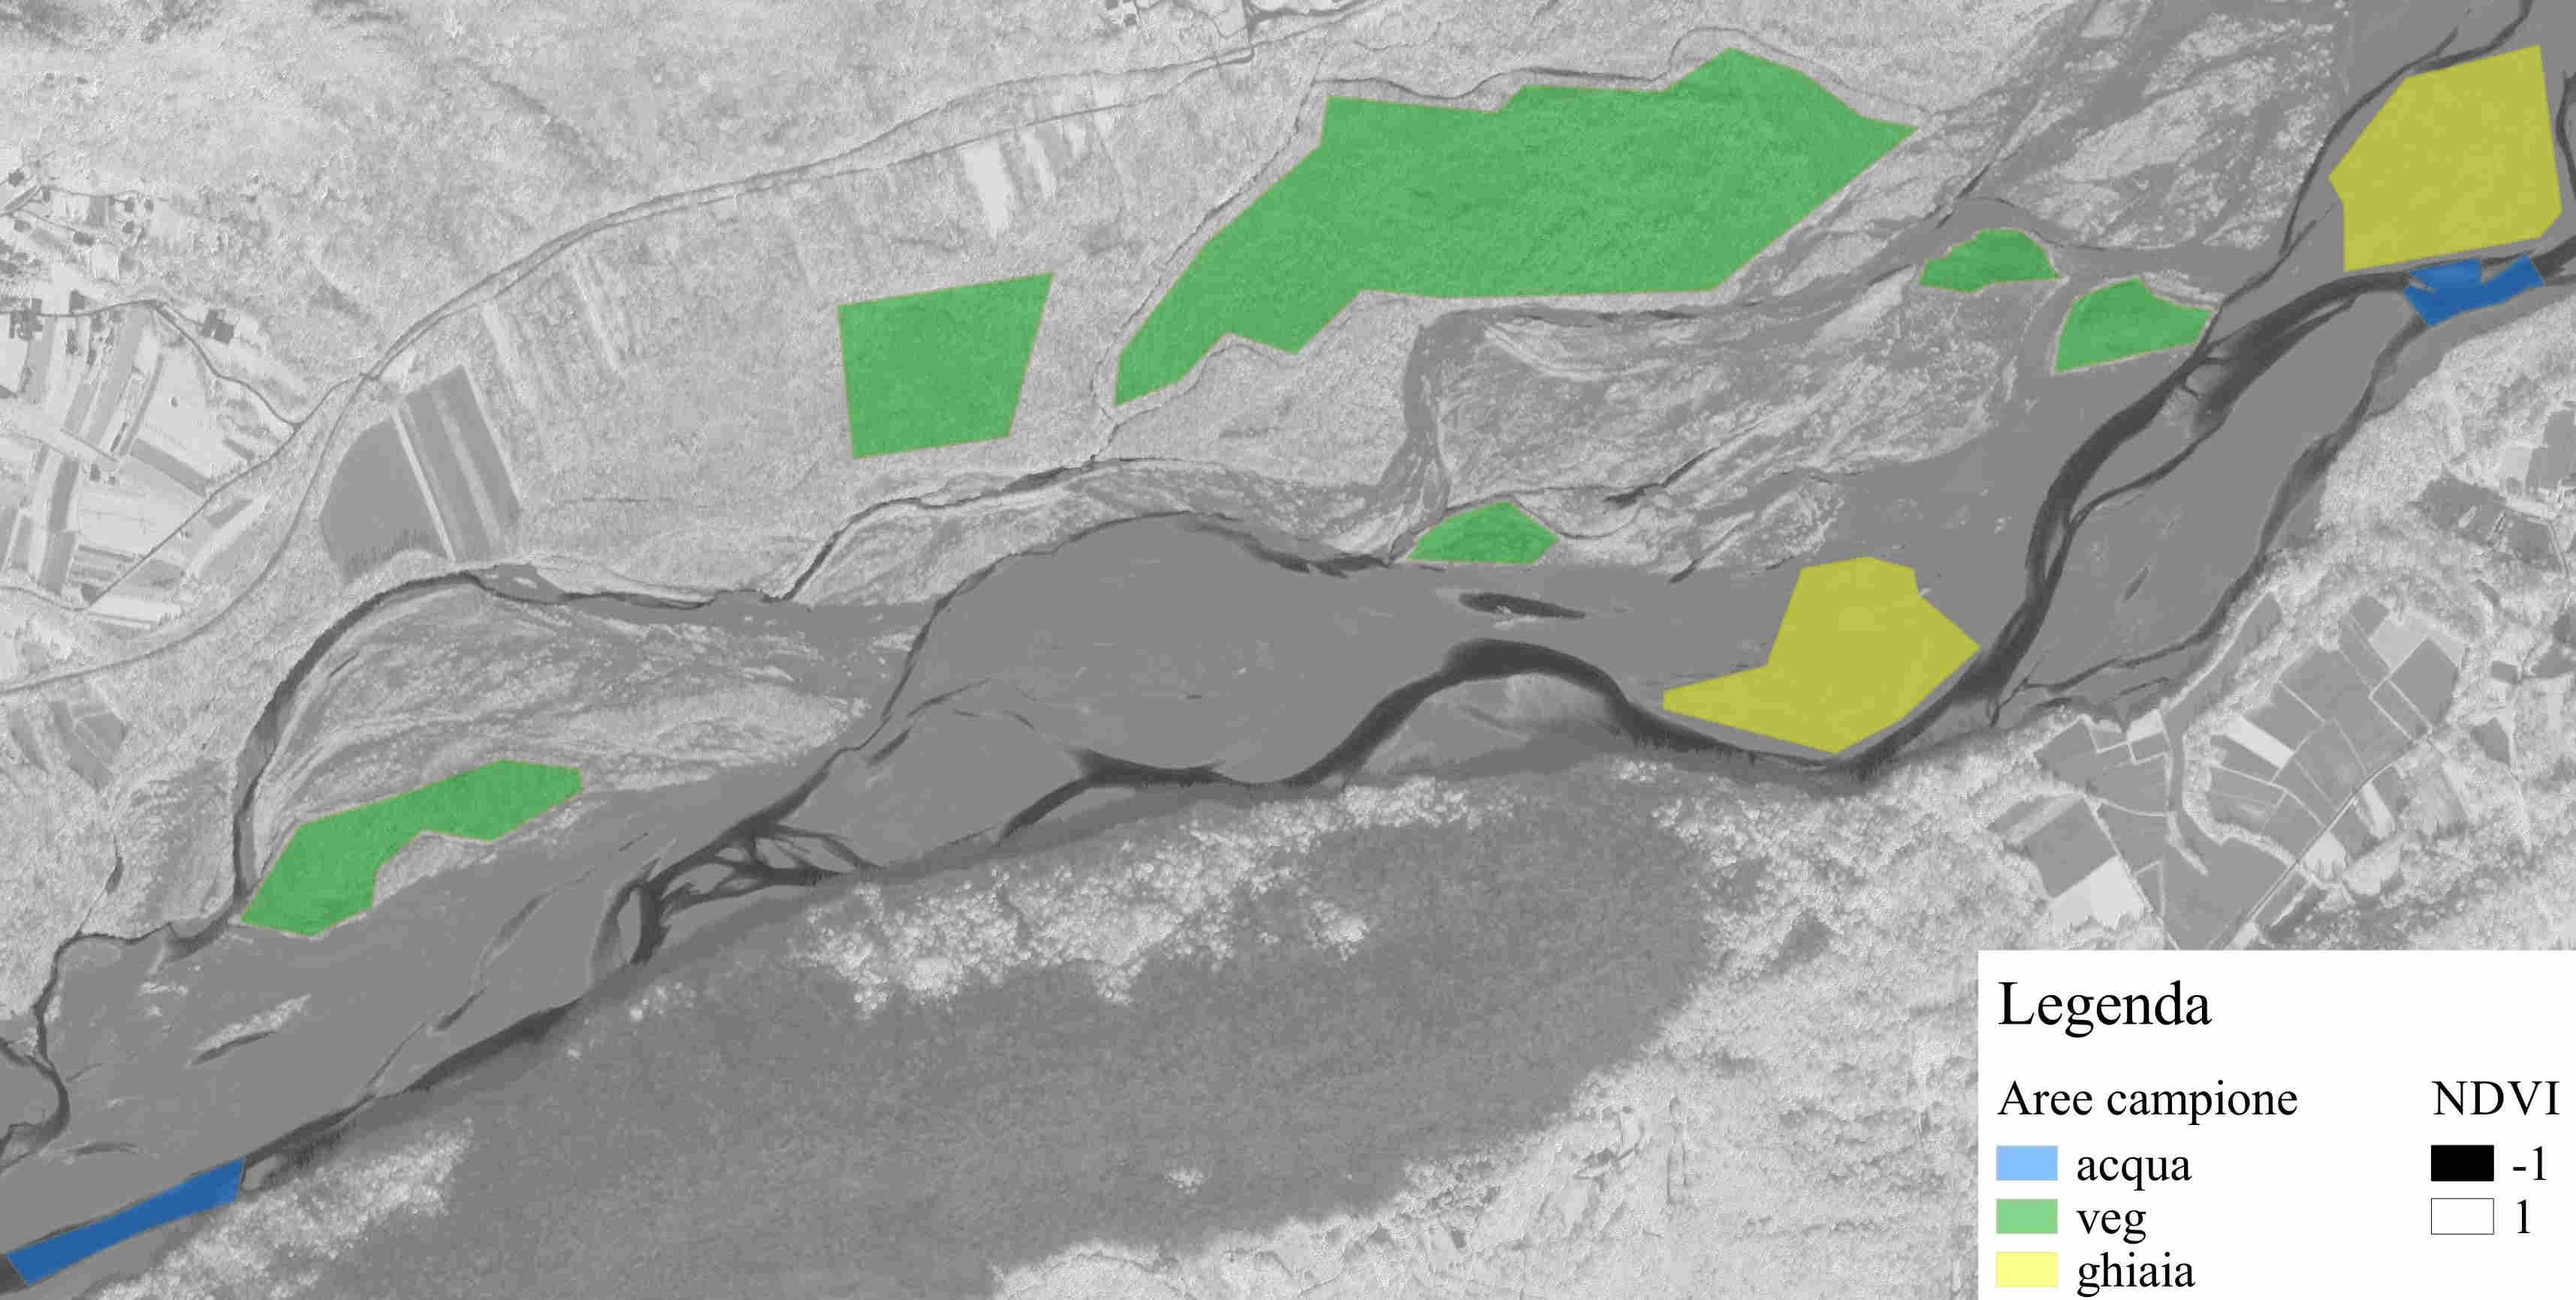
\includegraphics[width=\textwidth]{files/esempio_aree_campione_2014_10_31.jpeg}
		\caption[esempio di aree campione per calcolare la distribuzione dell'NDVI]{esempio di digitalizzazione di alcune aree campione per l'immagine \Pl{} del~2014-10-31; sullo sfondo la mappa dell'NDVI.}
		\label{fig:esempio-aree-campione}
	\end{figure}
	%
	%
\paragraph{Soglie NDVI}
Per ciascuna immagine si è osservata la distribuzione dell'NDVI in ogni classe tramite dei \emph{boxplot} (\cref{graph:percentili}): i \emph{boxplot} risultano essere nettamente separati gli uni dagli altri sia tra le scatole che tra i baffi; questo indica che le tre classi hanno distribuzioni di NDVI ben separate tra loro.
Ad esempio nella mappa dell'NDVI della \Pl{}~2014-10-31 il valore~\num{0.4} è sicuramente caratteristico della vegetazione e non dell'acqua; analogamente, valori superiori a~\num{0.2} sono certamente associati alla vegetazione, mentre valori inferiori sono associati a ghiaia o ad acqua.
% 
\begin{figure}[ht]
	\centering
	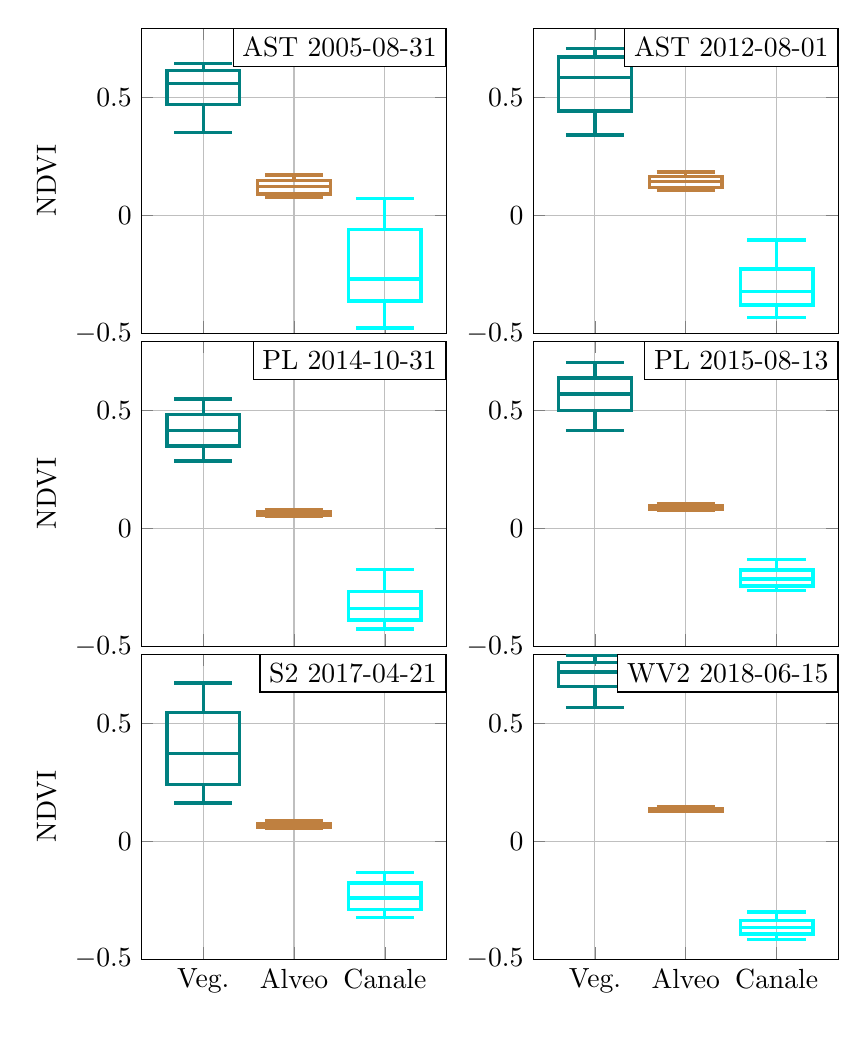
\begin{tikzpicture}
	\begin{groupplot}[
		group style = {
			group size = 2 by 3,
			ylabels at = edge left,
			x descriptions at = edge bottom,
			horizontal sep = 1.1cm,
			vertical sep = 0.1cm,
		},
		width = 0.45\textwidth,
		height = 0.45\textwidth,
		ylabel = NDVI,
		boxplot/draw direction = y,
		xtick = {1,2,3},
		xticklabels = {Veg., Alveo, Canale},
		ymax = 0.795,
		ymin = -0.50,
		grid = major,
	]
	\nextgroupplot % ASTER 2005-08-31
		\addplot+ [ % vegetazione
			teal, very thick,
			boxplot prepared = {
				lower whisker = 0.353656,
				lower quartile = 0.470411,
				median = 0.560063,
				upper quartile = 0.614701,
				upper whisker = 0.644957,
				},
        	]
        	coordinates {};
		\addplot+ [ % alveo attivo
			brown, very thick,
			boxplot prepared = {
				lower whisker = 0.077472,
				lower quartile = 0.091653,
				median = 0.122488,
				upper quartile = 0.149573,
				upper whisker = 0.171459,
				},
        	]
        	coordinates {};
		\addplot+ [ % canale
			cyan, very thick,
			boxplot prepared = {
				lower whisker = -0.477885,
				lower quartile = -0.362798,
				median = -0.269905,
				upper quartile = -0.058787,
				upper whisker = 0.072414,
				},
        	]
        	coordinates {};
        \node [fill = white, draw = black, anchor = north east] 
        	at (axis description cs: 1,1) {AST 2005-08-31};
	%------------------------------------------------------
	\nextgroupplot % ASTER 2012-08-01
		\addplot+ [ % vegetazione
			teal, very thick,
			boxplot prepared = {
				lower whisker = 0.341613,
				lower quartile = 0.444200,
				median = 0.586294,
				upper quartile = 0.672889,
				upper whisker = 0.709027,
				},
        	]
        	coordinates {};
		\addplot+ [ % alveo attivo
			brown, very thick,
			boxplot prepared = {
				lower whisker = 0.10506,
				lower quartile = 0.117969,
				median = 0.143631,
				upper quartile = 0.16549,
				upper whisker = 0.184871,
				},
        	]
        	coordinates {};
		\addplot+ [ % canale
			cyan, very thick,
			boxplot prepared = {
				lower whisker = -0.432201,
				lower quartile = -0.379825,
				median = -0.322239,
				upper quartile = -0.226459,
				upper whisker = -0.103914,
				},
        	]
        	coordinates {};
        \node [fill = white, draw = black, anchor = north east] 
        	at (axis description cs: 1,1) {AST 2012-08-01};
	%------------------------------------------------------
	\nextgroupplot % Pleiades 2014-10-31
		\addplot+ [ % vegetazione
			teal, very thick,
			boxplot prepared = {
				lower whisker = 0.286467,
				lower quartile = 0.350238,
				median = 0.415502,
				upper quartile = 0.483495,
				upper whisker = 0.549505,
				},
        	]
        	coordinates {};
		\addplot+ [ % alveo attivo
			brown, very thick,
			boxplot prepared = {
				lower whisker = 0.049796,
				lower quartile = 0.055794,
				median = 0.063049,
				upper quartile = 0.07173,
				upper whisker = 0.081427,
				},
        	]
        	coordinates {};
		\addplot+ [ % canale
			cyan, very thick,
			boxplot prepared = {
				lower whisker = -0.426415,
				lower quartile = -0.387978,
				median = -0.338308,
				upper quartile = -0.266515,
				upper whisker = -0.175373,
				},
        	]
        	coordinates {};
        \node [fill = white, draw = black, anchor = north east] 
        	at (axis description cs: 1,1) {PL 2014-10-31};
	%------------------------------------------------------
	\nextgroupplot % Pleiades 2015-08-13
		\addplot+ [ % vegetazione
			teal, very thick,
			boxplot prepared = {
				lower whisker = 0.415693,
				lower quartile = 0.5,
				median = 0.570359,
				upper quartile = 0.638507,
				upper whisker = 0.704044		
,
				},
        	]
        	coordinates {};
		\addplot+ [ % alveo attivo
			brown, very thick,
			boxplot prepared = {
				lower whisker = 0.075052,
				lower quartile = 0.080858,
				median = 0.087921,
				upper quartile = 0.096031,
				upper whisker = 0.106198,
				},
        	]
        	coordinates {};
		\addplot+ [ % canale
			cyan, very thick,
			boxplot prepared = {
				lower whisker = -0.262599,
				lower quartile = -0.244228,
				median = -0.214393,
				upper quartile = -0.176471,
				upper whisker = -0.132762,
				},
        	]
        	coordinates {};
        \node [fill = white, draw = black, anchor = north east] 
        	at (axis description cs: 1,1) {PL 2015-08-13};
	%------------------------------------------------------
	\nextgroupplot % Sentinel2 2017-04-21
		\addplot+ [ % vegetazione
			teal, very thick,
			boxplot prepared = {
				lower whisker = 0.163722,
				lower quartile = 0.241916,
				median = 0.374344,
				upper quartile = 0.548241,
				upper whisker = 0.672782,
				},
        	]
        	coordinates {};
		\addplot+ [ % alveo attivo
			brown, very thick,
			boxplot prepared = {
				lower whisker = 0.056176,
				lower quartile = 0.061278,
				median = 0.067681,
				upper quartile = 0.076396,
				upper whisker = 0.089304,
				},
        	]
        	coordinates {};
		\addplot+ [ % canale
			cyan, very thick,
			boxplot prepared = {
				lower whisker = -0.322237,
				lower quartile = -0.288822,
				median = -0.239533,
				upper quartile = -0.177094,
				upper whisker = -0.131119,
				},
        	]
        	coordinates {};
        \node [fill = white, draw = black, anchor = north east] 
        	at (axis description cs: 1,1) {S2 2017-04-21};
	%------------------------------------------------------
	\nextgroupplot % WorldView2 2018-06-15
		\addplot+ [ % vegetazione
			teal, very thick,
			boxplot prepared = {
				lower whisker = 0.569665,
				lower quartile = 0.657917,
				median = 0.719523,
				upper quartile = 0.759148,
				upper whisker = 0.791594,
				},
        	]
        	coordinates {};
		\addplot+ [ % alveo attivo
			brown, very thick,
			boxplot prepared = {
				lower whisker = 0.126214,
				lower quartile = 0.129661,
				median = 0.13373,
				upper quartile = 0.138542,
				upper whisker = 0.149326,
				},
        	]
        	coordinates {};
		\addplot+ [ % canale
			cyan, very thick,
			boxplot prepared = {
				lower whisker = -0.416974,
				lower quartile = -0.392405,
				median = -0.365385,
				upper quartile = -0.335135,
				upper whisker = -0.29979,
				},
        	]
        	coordinates {};
        \node [fill = white, draw = black, anchor = north east] 
        	at (axis description cs: 1,1) {WV2 2018-06-15};
	\end{groupplot}
\end{tikzpicture}

	\caption[\emph{boxplot} dell'NDVI nelle aree campione in quattro immagini satellitari]{\emph{boxplot} dell'NDVI nelle aree campione in quattro immagini satellitari; i baffi indicano il $10_\mathrm{mo}$ e il $90_\mathrm{mo}$ percentile, gli estremi della scatola rappresentano il $25_\mathrm{mo}$ e il $75_\mathrm{mo}$ percentile, la linea nella scatola è la mediana.}
	\label{graph:percentili}
\end{figure}
%
\\
Da tali grafici sono state ottenute delle soglie di NDVI per classificare le immagini satellitari (\cref{tab:ndvi-soglia}); per l'immagine \WV{} la soglia che distingue vegetazione da alveo attivo è maggiore. 
Le soglie sono leggermente maggiori rispetto a quanto riportato in letteratura \squarecites{Bertoldi:2011-ASTER}{Henshaw:2013-LandSat} poiché in questo modo c'è una maggior corrispondenza con i dati utilizzati per validare il processo (riportati di seguito).
%
\begin{table}[ht]
	\centering
	\begin{tabular}{
		c 
		S[table-format=1.2]@{\,}
		c@{\,}
		c@{\,}
		c@{\,}
		S[table-format=1.2]
		S[table-format=1.2]@{\,}
		c@{\,}
		c@{\,}
		c@{\,}
		S[table-format=1.2]
		}
		\toprule
		&	\multicolumn{5}{c}{\textbf{Soglie AST PL S2}}	&	\multicolumn{5}{c}{\textbf{Soglie WV2}}	\\
		\midrule
		Vegetazione		&	0.25	&	$\leq$	&	NDVI	&			&		& 	0.30	&	$\leq$	&	NDVI	&			& 	\\
		Alveo attivo	&	0.00	&	$\leq$	&	NDVI	&	$<$		&	0.25	&	0.00	&	$\leq$	&	NDVI	&	$<$		&	0.30	\\
		Canale			&		&			&	NDVI	&	$<$		&	0.00	&		&			&	NDVI	&	$<$		&	0.00	\\
		\bottomrule
	\end{tabular}
	\caption[soglie NDVI]{soglie di NDVI per la classificazione delle immagini satellitari.}
	\label{tab:ndvi-soglia}
\end{table}
%
%
\paragraph{Isole e \emph{Floodplain}}
La maschera computazione individuata è unica per tutte le immagini in quanto è definita come l'inviluppo degli alvei attivi che si sono succeduti dal~2000 al~2018.
Il problema di questo approccio è che la copertura riparia delle isole non viene distinta da quella delle sponde.
Inoltre, a causa della bassa risoluzione delle immagini satellitari, i canali che separano isole molto prossime alla \emph{floodplain} dalle sponde stesse non vengono individuati e tali isole sembrano far completamente parte della \emph{floodplain}.
\\ 
Come soluzione è stata ideata una procedura semi-automatica che, con il supporto di Google Earth, divida la classe della vegetazione in \emph{floodplain} e isole. 
Tale procedura, sfruttando il fatto che le isole sono completamente circondate dalla ghiaia dell'alveo durante periodi di magra, classifica inizialmente la vegetazione più esterna come sponda;
poi corregge alcune celle della \emph{floodplain} convertendole in celle dell'alveo, separando nettamente le isole dalle sponde (\cref{fig:isola-divisa-floodplain}).
Le classi delle isole, delle sponde e delle celle corrette sono state aggiunte alla classificazione.
%
\begin{figure}
	\centering
	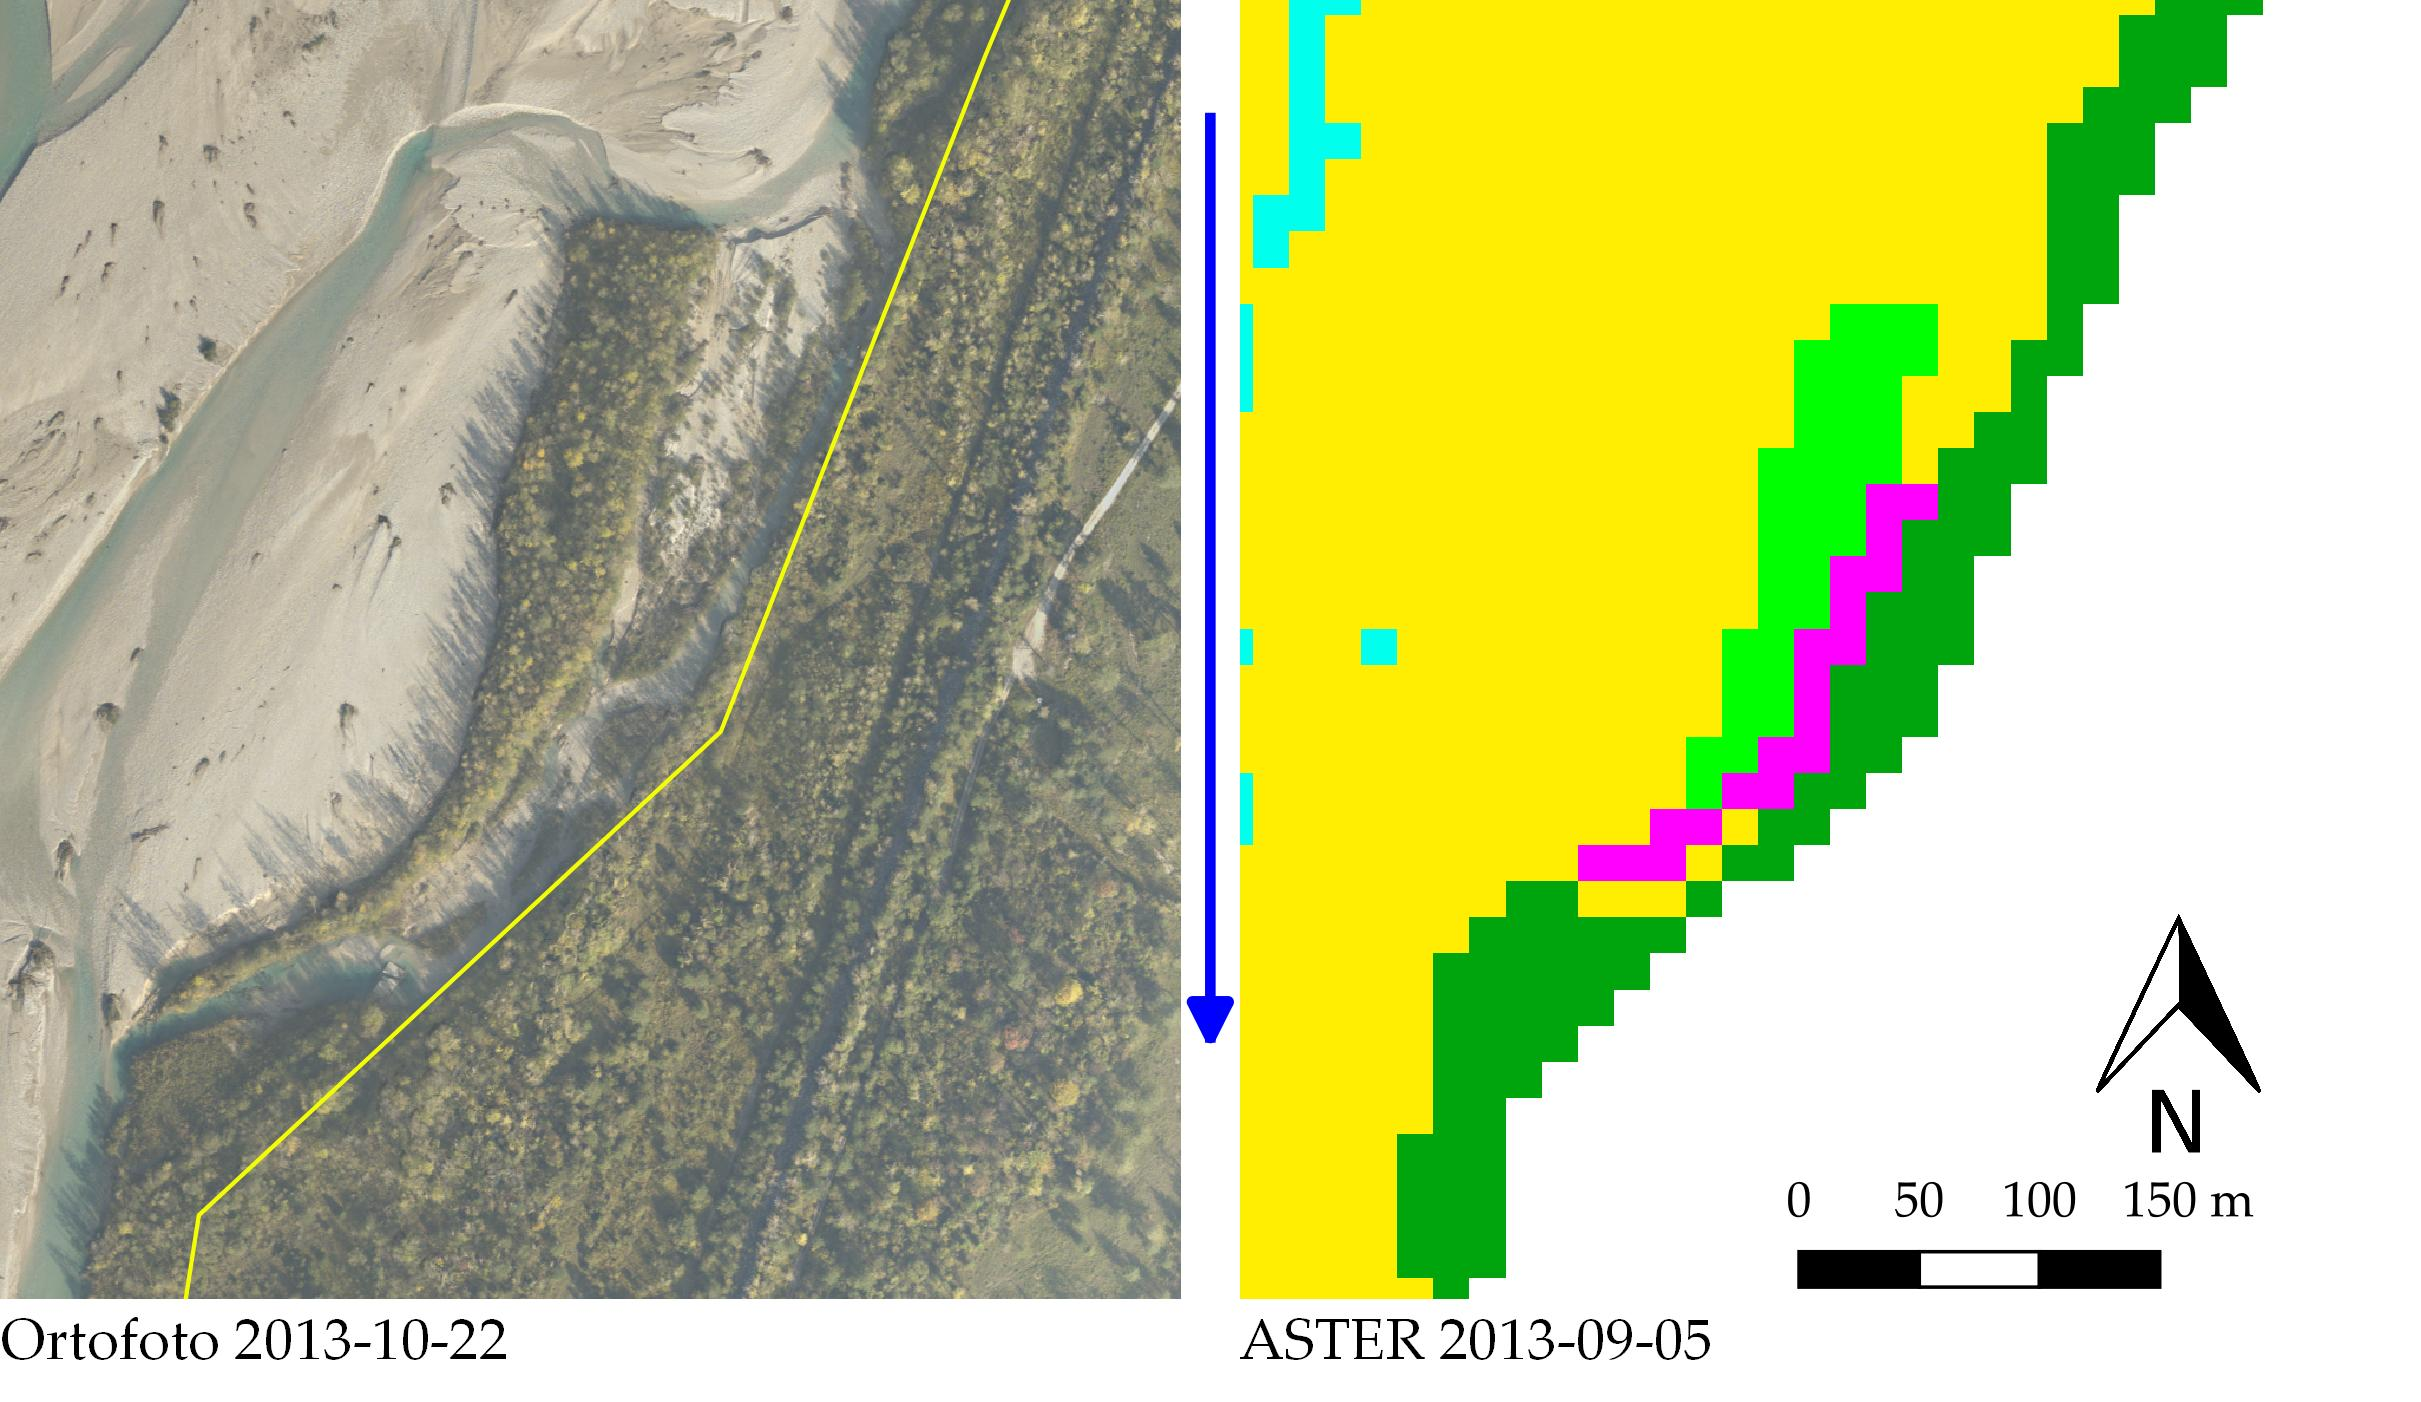
\includegraphics[width = \textwidth]{files/isola_divisa_floodplain.jpeg}
	\caption[esempio di correzione per dividere un'isola dalla sponda]{a sinistra si vede sull'ortofoto un'isola divisa dalla sponda tramite un canale (in giallo è mostrato il limite della maschera computazionale); a destra si vede la stessa isola (verde chiaro) nell'immagine \AST{} temporalmente più vicina che è stata corretta (fucsia) per distinguerla dalla \emph{floodplain} (verde scuro); l'isola è circondata da ghiaia (giallo) e da acqua (azzurro).}
	\label{fig:isola-divisa-floodplain}
\end{figure}
%
%
%
\paragraph{Nuvole e nodata}
Alcune immagini presentano una lieve copertura nuvolosa che si estende nella maschera; queste zone sono state manualmente delimitate poiché presentano valori NDVI alterati.
\\
Altre immagini hanno un'estensione limitata rispetto alla maschera; questo porta ad avere aree prive di dati (\texttt{nodata}).
\\
Alla classificazione sono state aggiunte la classe delle nuvole e dei \texttt{nodata}.
%
%
\paragraph{Classificazione finale dei tratti}
La \cref{tab:class_tratti} mostra le classi in cui è stato classificato ognuno dei 23~tratti; la \cref{fig:class_is_fl} ne mostra un esempio.
%
\begin{table}[ht]
	\centering
	\begin{tabular}{
		c 
		c
		}
		\toprule
		\textbf{Macroclasse}	&	\textbf{Classe}	\\
		\midrule
		Vegetazione		&	Isola	\\
						&	Floodplain	\\
		Alveo attivo	&	Cella corretta	\\
						&	Ghiaia	\\
						&	Canale	\\
		Altro			&	Nuvola	\\
						&	Nodata	\\
		\bottomrule
	\end{tabular}
	\caption[classificazione dell'area dei tratti]{classificazione finale dell'area di ogni tratto all'interno della maschera computazionale.}
	\label{tab:class_tratti}
\end{table}
%
\begin{figure}[ht]
	\centering
	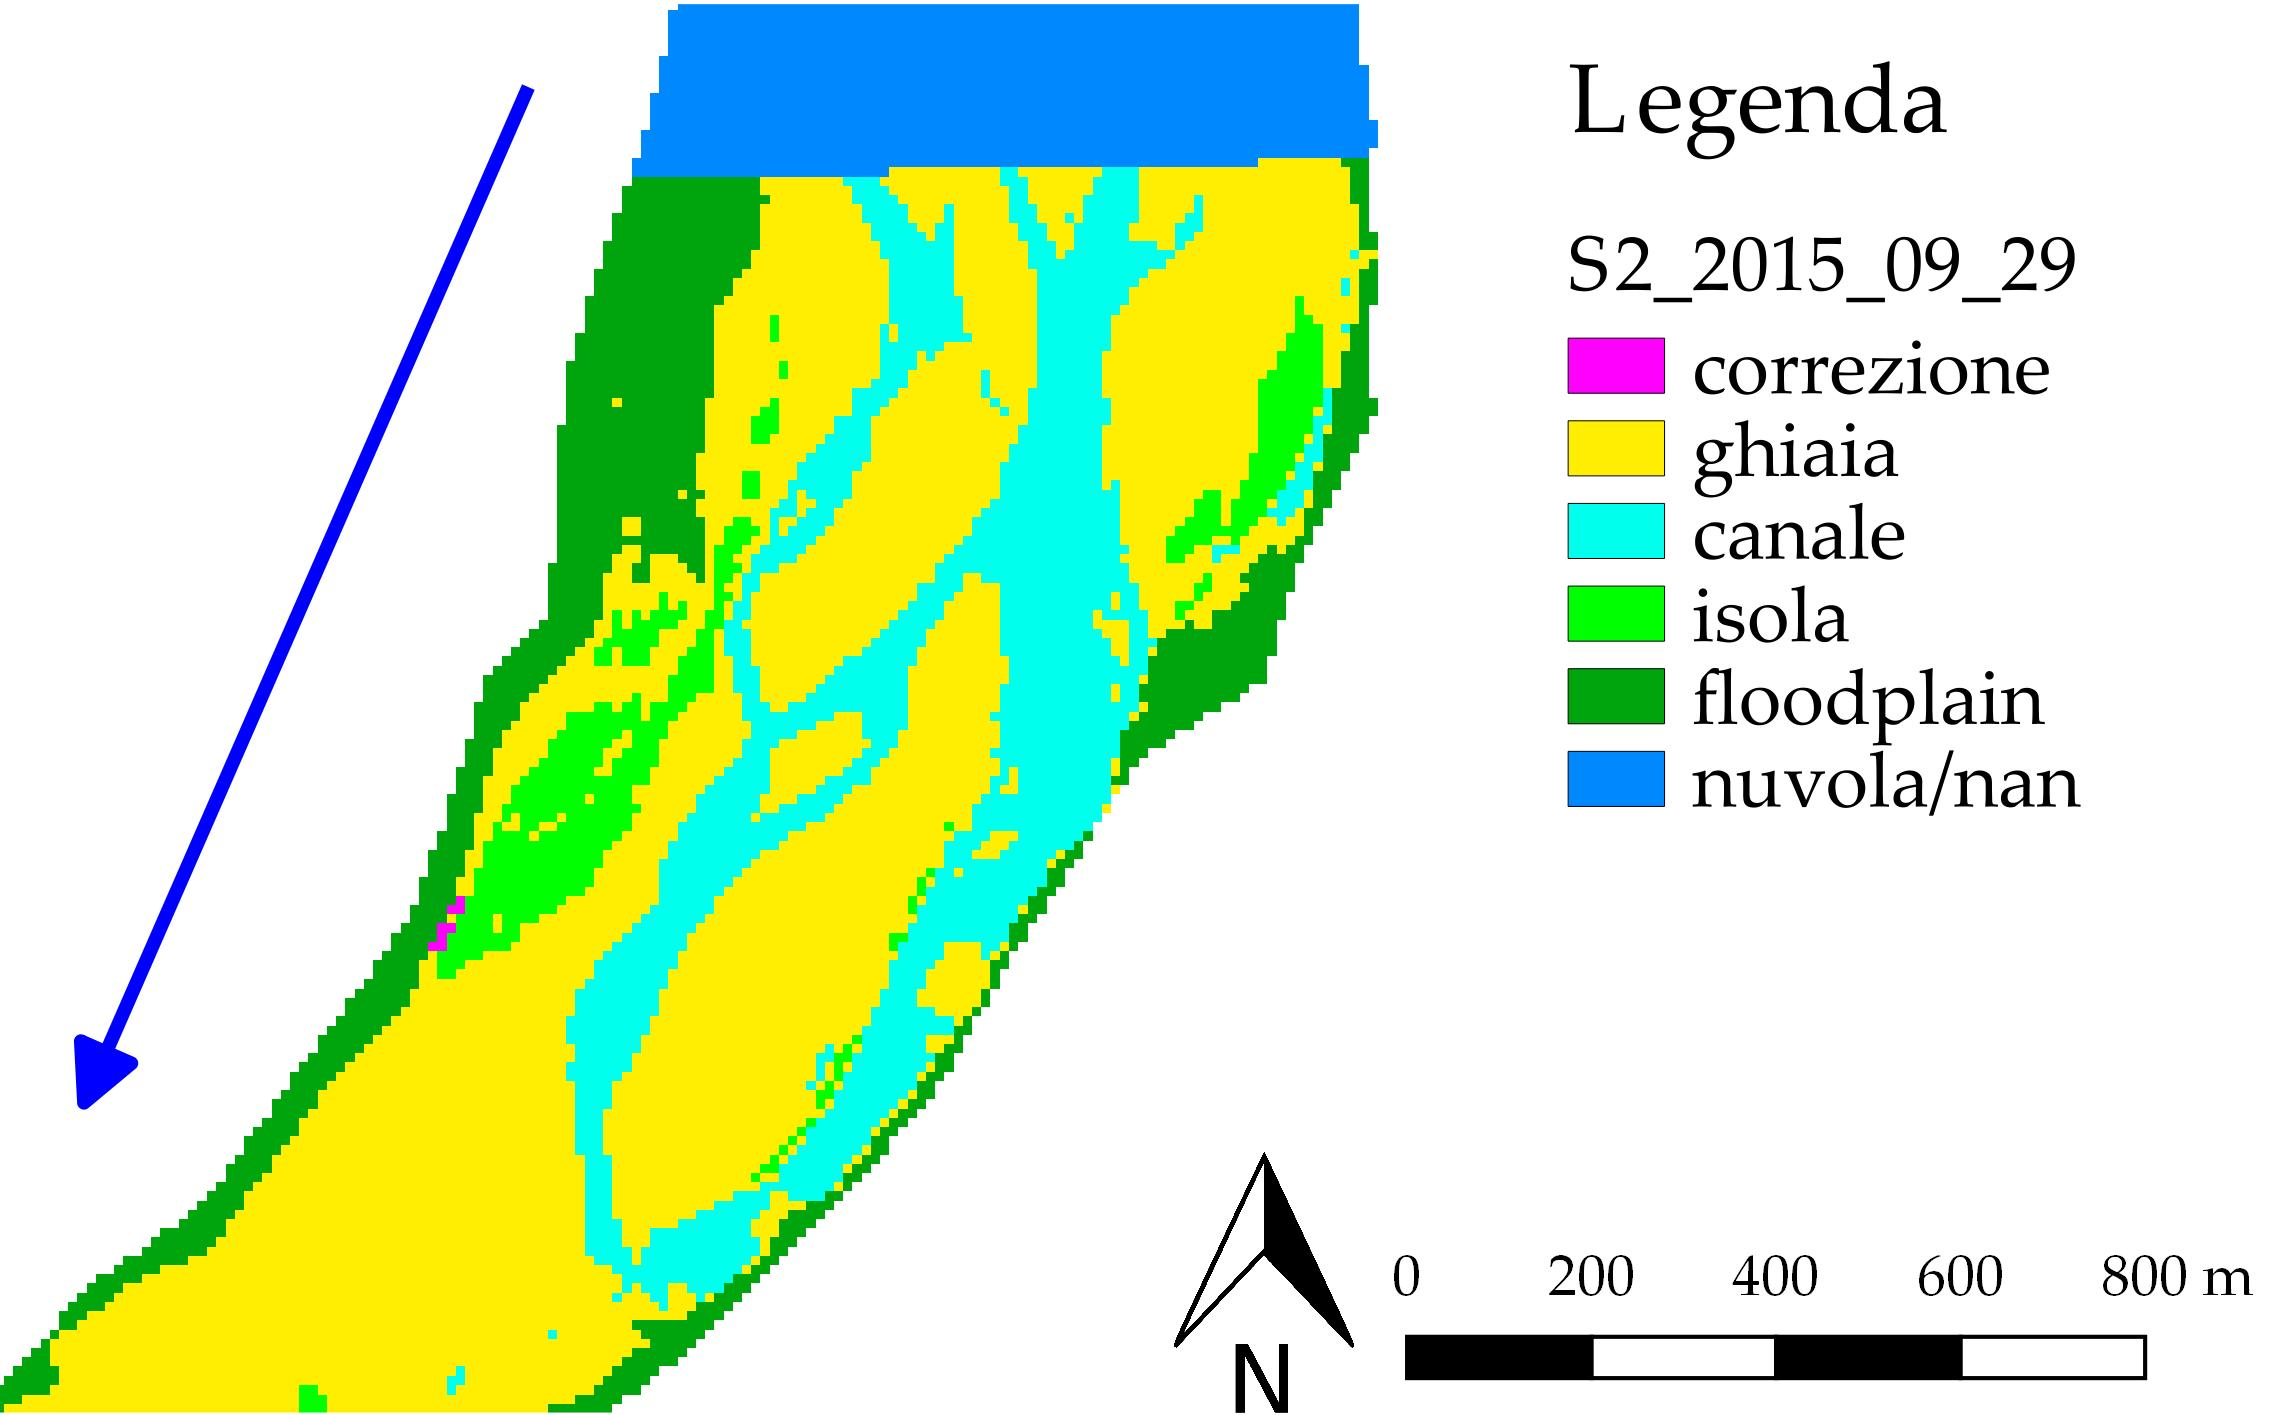
\includegraphics[width=\textwidth]{files/esempio_class_is_fl.jpeg}
	\caption[esempio della classificazione dell'area dei tratti]{esempio della classificazione dell'area dei tratti; le zone raffigurate sono rispettivamente a monte dell'isola di Cornino (in corrispondenza del monte Prat) e in corrispondenza della confluenza del Fella.}
	\label{fig:class_is_fl}
\end{figure}
%
%
%
\paragraph{Validazione}
Per controllare che la procedura restituisca risultati veritieri, si è confrontata la classificazione semi-automatica del 2011-10-02 con la classificazione eseguita manualmente da \squarecite{Surian:2015} nei tratti \numrange[range-phrase={$\div$}]{6}{12} (dal ponte autostradale di Braulins alla stretta di Pinzano).
Le mappe di classificazione del 2005-08-30, 2010-09-29, 2013-09-05 sono state confrontate con i CHM ricavati dai rilievi aerei LiDAR eseguiti nei corrispondenti anni su alcune porzioni dei tratti \numrange[range-phrase={$\div$}]{6}{12}.
Le immagini in \cref{fig:validazione-class-is-fl} mostrano alcuni confronti visuali tra classificazione semi-automatica e le immagini usate per la validazione.
Tra i rilievi LiDAR e le immagini \AST{} non hanno avuto luogo particolari eventi di piena, così come tra l'ortofoto del~2011 e la corrispondente immagine \AST{}.
%	
\begin{figure}
	\centering
	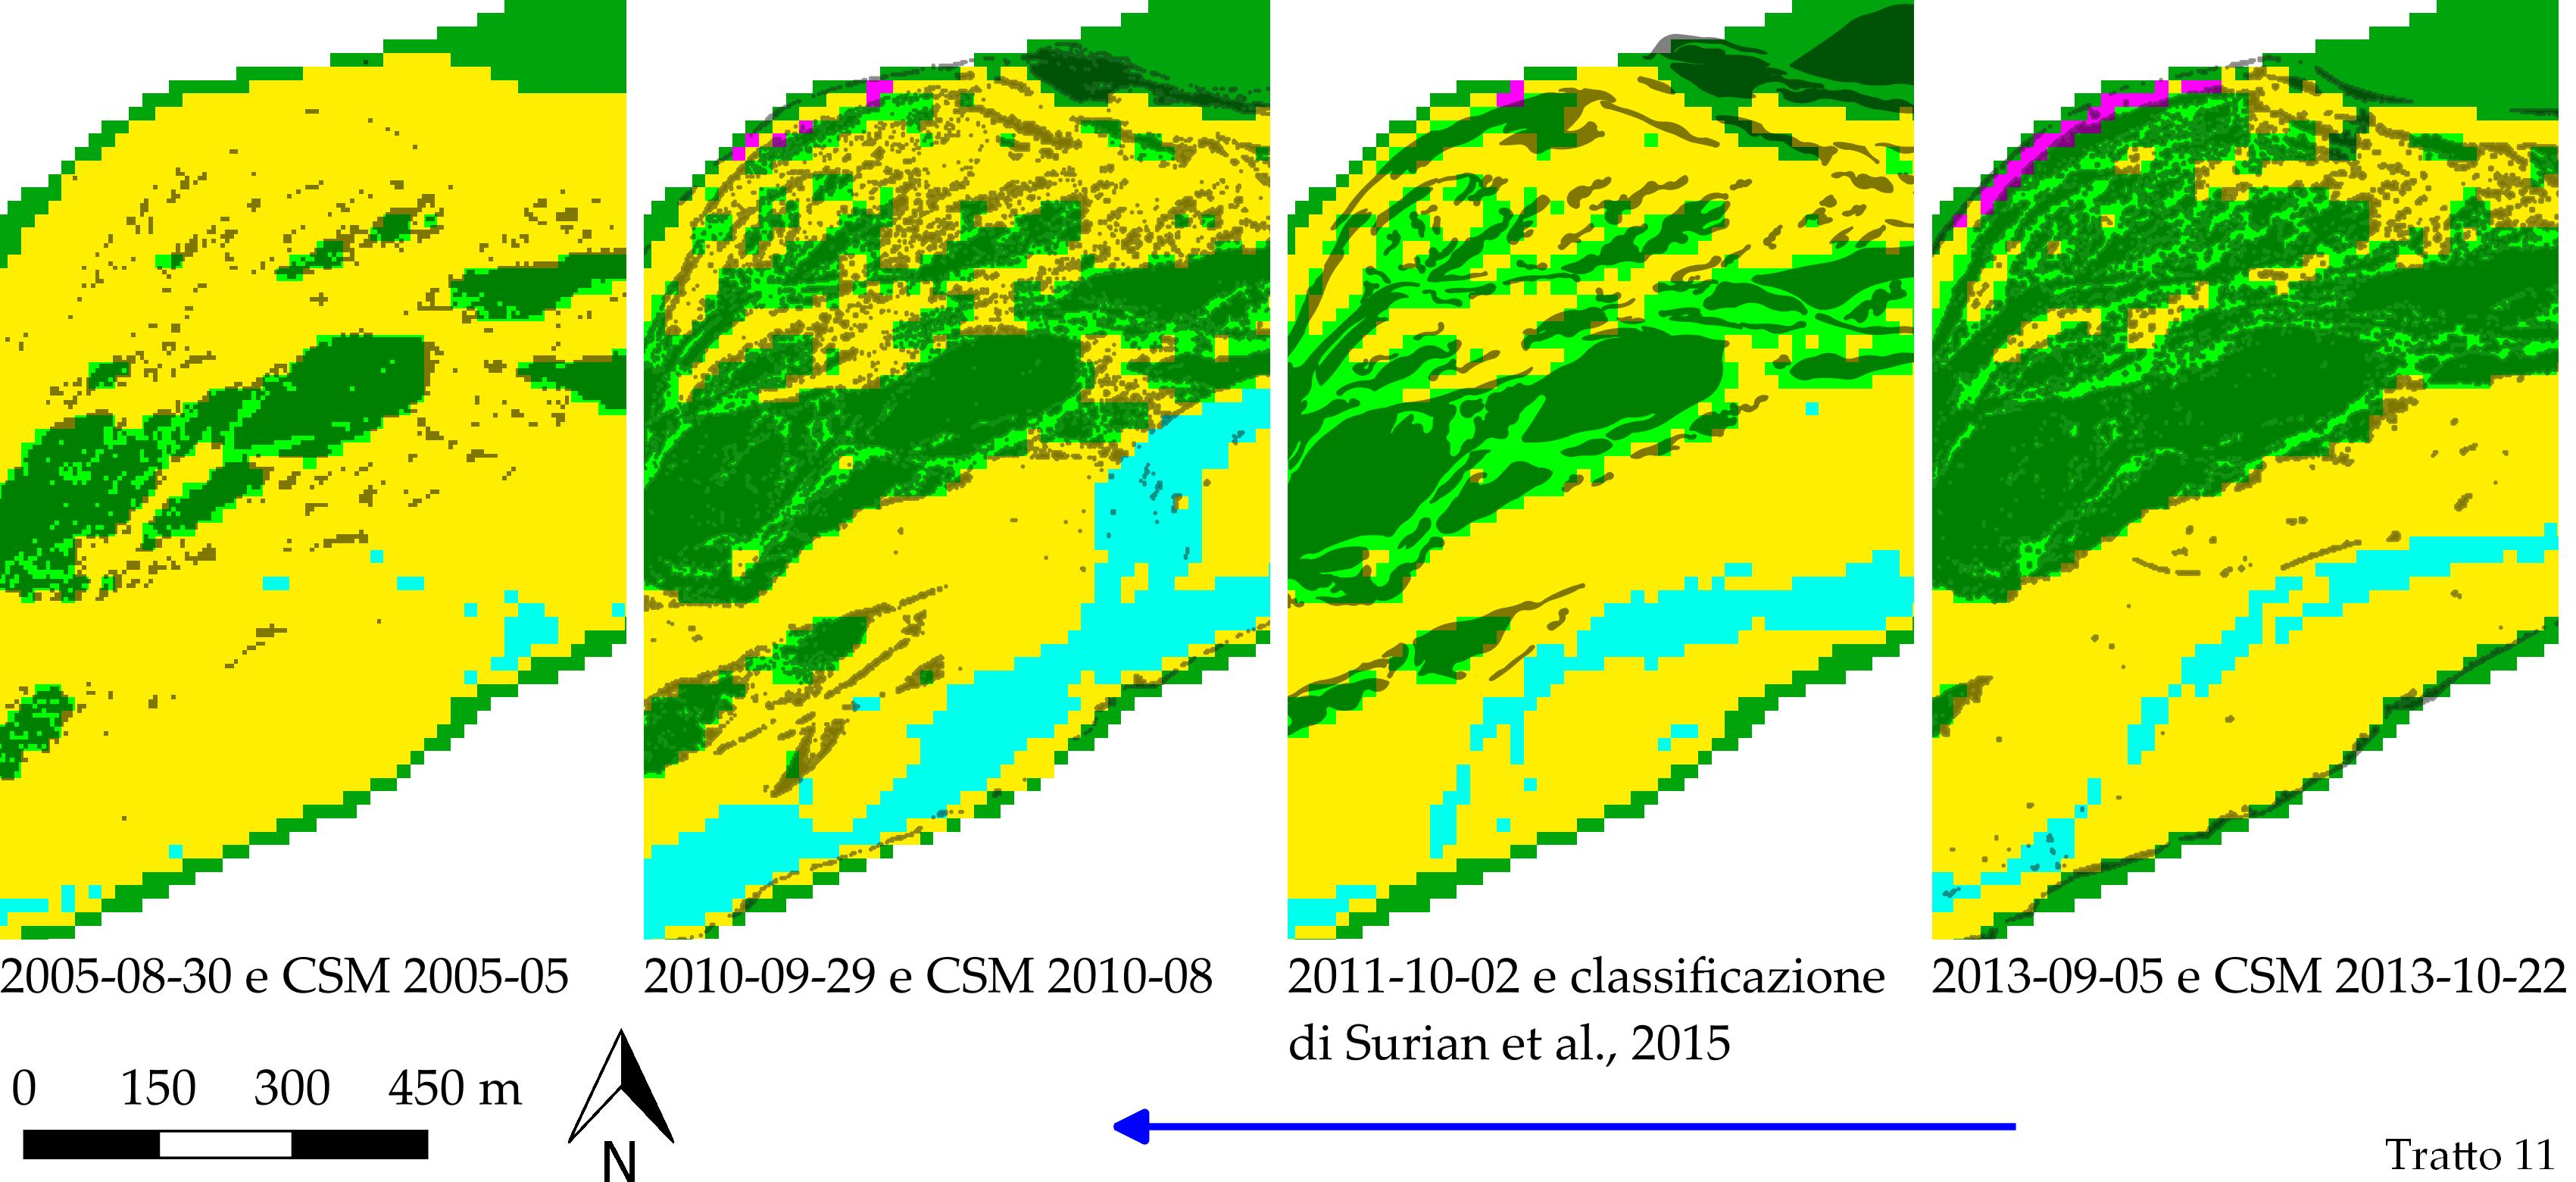
\includegraphics[width=\textwidth]{files/class_mia_vs_surian_chm.jpeg}
	\caption[validazione visuale della classificazione dell'alveo]{confronto tra le mappe di classificazione dell'alveo (sullo sfondo), i CHM ottenuti con rilievi aerei LiDAR e la classificazione manuale eseguita in \squarecite{Surian:2015} (in rosso semi-trasparente); le aree di sovrapposizione di rosso e verde chiaro indicano la corrispondenza tra la classificazione semi-automatica e i dati esterni; i colori indicano le isole (verde chiaro), le sponde (verde scuro), l'alveo (giallo), i canali (azzurro) e le celle corrette per distinguere le isole dalle sponde (fucsia).}
	\label{fig:validazione-class-is-fl}
\end{figure}
%
\begin{aenumerate}
	\item La classificazione manuale distingue la copertura arborea in tre tipi: alta, media e bassa.
	Le isole sono definite come le zone con alberi con un'area di \SI{\sim 100}{\m\tothe{2}}; nella presente tesi invece le isole sono definite come zone più o meno vegetate separate dalle sponde e circondate completamente da ghiaia e acqua, e questo porta a considerare come isole aree più ampie.
	\\
	La risoluzione minore delle immagini satellitari (principalmente a~\SI{10}{\m} o~\SI{15}{\m}) rispetto all'ortofoto (\SI{0.1}{\m}) permette di osservare macchie di vegetazione anziché i singoli alberi, delineando più nettamente il contorno delle isole maggiori; tuttavia le isole più piccole (con estensione minore di una cella) non sono individuate.
	\\
	Questa differenza nei metodi e nella definizione di isola porta ad una differenza del~\SI{-14}{\percent} dell'areale delle isole nella classificazione manuale rispetto a quella semi-automatica.
	%
	\item I CHM mostrano l'altezza della copertura arborea; dove questa altezza non è nulla, è presente vegetazione.
	La misura dell'altezza non si basa sul riconoscimento di un colore, come nella classificazione semi-automatica e manuale, ma sfrutta la riflessione di raggi laser da parte delle superfici, quali terreno e alberi; quindi i CHM costituiscono una fonte di validazione ben distinta dalla classificazione manuale.
	\\
	La somma delle aree con altezza della vegetazione non nulla nell'alveo costituisce l'area delle isole individuata per ogni CHM; rispetto alla classificazione semi-automatica, le differenze sono del \SIlist[list-separator = {, }, list-final-separator = { e }, retain-explicit-plus]{+22;+9;-3}{\percent} per i CHM del~2005, 2010 e~2013 rispettivamente.
\end{aenumerate}
%
Nel grafico in \cref{graph:validazione-class-is-fl} si vede l'areale delle isole nelle mappe di classificazione dell'alveo del~2005, 2010, 2011 e~2013 rispetto all'areale dalle mappe usate come validazione.
%
\begin{figure}
	\centering
	\tikzsetnextfilename{validazione_class_is_fl}
\begin{tikzpicture}
	\begin{axis}[
		width = 0.5\textwidth,
		height = 0.5\textwidth,
		xlabel = {Isole da NDVI \si{[\kilo\m\tothe{2}]}},
		ylabel = {Isole da CHM e class. manuale \si{[\kilo\m\tothe{2}]}},
		grid = major,
		]        
		\addplot[
			scatter,
			green!75!black,
			only marks,
			nodes near coords,
			%point meta = explicit symbolic,
			]
        	table [x expr = \thisrow{mie} / 1000000, y expr = \thisrow{CHM_Surian} / 1000000, point meta = \thisrow{anno}] {graphics/data/validazione_class_is_fl.txt};
        
		\addplot[
			blue,
			dashed,
			no markers,
			domain = 0.5:1.1,
			samples = 2,
			]
        	{x};
	\end{axis}
\end{tikzpicture}

	\caption[validazione della classificazione considerando le aree delle isole]{areale delle isole secondo la classificazione semi-automatica messa a confronto con quella secondo tre rilievi LiDAR e con una classificazione manuale \squarecite{Surian:2015}; la retta tratteggiata indica la situazione ideale in cui l'area delle isole ottenuta dalle immagini satellitari corrisponde a quella ottenuta con gli altri metodi; si rammenta che in ogni anno è stato considerato il tratto coperto dai CHM e dalla classificazione manuale.}
	\label{graph:validazione-class-is-fl}
\end{figure}
%
\\
C'è una certa differenza tra le isole individuate tramite la classificazione semi-automatica e quelle ottenute attraverso la classificazione manuale e i CHM, dovuta molto probabilmente ai diversi metodi di misura.
Da una parte, le mappe usate per la validazione mostrano isole con aree molto più piccole delle celle delle immagini satellitari e i CHM possono individuare come albero qualunque oggetto che si trovi sopra al terreno, come accumuli di legno o piloni della rete elettrica; dall'altra, tali mappe non classificano come isola le piccole aree ghiaiose o con vegetazione rada situate nel mezzo di isole ben sviluppate, come invece fa la classificazione semi-automatica.
\\
La differenza è stata calcolata solo per una piccola parte del tratto di studio poiché i dati di validazione non erano particolarmente estesi spazialmente.
In questa zona non sembra che la classificazione semi-automatica sovrastimi o sottostimi l'areale delle isole, ma che si collochi in una condizione intermedia.
\\
A fronte di quanto esposto, si ritiene che la classificazione eseguita sia sufficientemente valida.


\subsection{Larghezza}
Con i dati di classificazione dell'alveo è possibile calcolare la larghezza media~$B$ dell'alveo attivo, esprimibile semplicemente come il rapporto dell'area dell'alveo di ogni tratto (somma dell'alveo attivo e delle isole) rispetto alla sua lunghezza:
%
\begin{equation}
	\label{eq:larghezza-tratto}
	B = \frac{\text{Area alveo}}{Lunghezza} 
	\quad 
	\si{[\m]}
	\quad.
\end{equation}
% 
La lunghezza di un tratto è definita come la linea che,  seguendo la corrente, congiunge la sezione di monte a quella di valle; è unica per ogni tratto; il tratto più breve è l'8 (\SI{1260}{\m}) e il più lungo è il~17 (\SI{6340}{\m}).
In quanto le sezioni che definiscono ciascun tratto non cambiano nel tempo, anche la relativa lunghezza non cambia; l'area dell'alveo attivo, al contrario, può variare da un'immagine all'altra. 
%
%
\subsection{Potenza della corrente}
La potenza della corrente per unità di larghezza $\Omega$ in \si{[\watt\per\meter\tothe{2}]} è definita come:
%
\begin{equation}
	\label{eq:omega}
	\Omega = \frac{\rho \, g \, Q \, i_f}{B}
	\quad
	\si{[\watt\per\meter\tothe{2}]}
\end{equation}
%
dove:
%
\begin{itemize}
	\item $\rho$ è la densità dell'acqua, pari a \SI{1000}{\kilo\g\per\meter\tothe{3}};
	\item $g$ è l'accelerazione di gravità, pari a \SI{9.81}{\m\per\s\tothe{2}};
	\item $Q$ è la portata fluente nel canale misurata in \si{[\m\tothe{3}\per\s]};
	\item $i_f$ è la pendenza in \si{[\m\per\m]};
	\item $B$ è la larghezza del canale in \si{[\m]}.
\end{itemize}
%

Per ottenere la \emph{stream power} si è prima ottenuta la pendenza media di ogni tratto grazie al DEM del 2009 nella seguente maniera:
%
\begin{aenumerate}
	\item si è definita una coordinata curvilinea che segue il corso principale del fiume;
	\item sono state considerate le quote in tutti i punti sopra i quali scorre la coordinata curvilinea;
	\item è stata effettuata una regressione lineare tra la coordinata curvilinea e le quote raggruppando i tratti quattro a quattro (tranne per l'ultimo gruppo, formato dai tratti 21, 22 e 23);
	\item il coefficiente angolare della retta rappresenta la pendenza del gruppo di 4 tratti.
\end{aenumerate}
%
Il risultato è riportato nella \cref{tab:pendenza}.
%
\begin{table}
	\centering
	\begin{tabular}{
		S[list-separator={, }, list-final-separator={ e }]
		S[table-format=1.2]
	}
		\toprule
		\multicolumn{1}{c}{Tratti}	&	\multicolumn{1}{c}{Pendenza \si{[\percent]}}	\\
		\midrule
		\numlist{1;2;3;4}	&	0.52	\\
		\numlist{5;6;7;8}	&	0.48	\\
		\numlist{9;10;11;12}	&	0.23	\\
		\numlist{13;14;15;16}	&	0.40	\\
		\numlist{17;18;19;20}	&	0.31	\\
		\numlist{21;22;23}	&	0.25	\\
		\bottomrule
	\end{tabular}
	\caption[pendenze dei tratti]{pendenze dei tratti.}
	\label{tab:pendenza}
\end{table}
%
\\
In quanto modificazioni della pendenza avvengono in periodi di tempo di anni soprattutto in seguito ad eventi naturali e non di apporto o asporto di sedimenti, che non sono avvenuti in maniera diffusa ed intensa durante gli ultimi due decenni, si considera la pendenza ottenuta come rappresentativa e costante nel periodo di studio.
In più, questi valori sono in accordo con quanto presente in letteratura \squarecites{Arscott:2002-habitat-dynamics}{Gurnell:2006-omega}{Bertoldi:2010-d50}{Sitzia:2016-d50}.

Mentre la larghezza $B$ è nota per quasi ogni tratto in ogni immagine, la portata $Q$ non è nota.
Secondo quanto descritto nella sezione \ref{sec:descr-area-studio}, la percentuale di area di bacino drenante in ogni tratto può fornire un'informazione sulla portata fluente in quanto quest'ultima è approssimativamente proporzionale all'area drenante.
\\
Poiché i dati di livello alla stazione idrometrica di Villuzza rappresentano in maniera affidabile l'entità delle piene, si è deciso di riferire l'area drenante di ogni bacinoin ogni tratto rispetto a quella del tratto~12, posto immediatamente a monte del sensore idrometrico (si veda la \cref{fig:overview-sat} e la \cref{fig:23-tratti}).
In questo modo si suppone che, durante le piene, in ogni tratto scorra una portata che è proporzionale alla percentuale di bacino drenante rispetto al bacino sotteso alla stazione idrometrica; tale percentuale è minore dell’unità a monte della stazione, mentre è maggiore all’unità a valle della stazione.
Per definire l’area drenante in ogni tratto sono stati utilizzati i dati riguardo gli affluenti mostrati nell’introduzione.
\\
L'equazione~\eqref{eq:omega-finta} definisce formalmente la potenza della corrente fittizia utilizzata nel presente lavoro.
Per comodità e semplicità, la definizione e nomenclatura della potenza della corrente originale viene sostituita dalla potenza della corrente fittizia.
La nuova $\Omega$ si misura in \si{[\newton\per\m\tothe{4}]}.
%
\begin{equation}
	\label{eq:omega-finta}
	\Omega = \frac{A_\mathrm{tr}}{A_\mathrm{rif}} \, \frac{\rho \, g \, i_f}{B}	
	\quad
	\si{[\newton\per\m\tothe{4}]} 
\end{equation}
%
dove:
%
\begin{itemize}
	\item $A_\mathrm{tr}$ è l'area drenante di ogni tratto in \si{[\m\tothe{2}]};
	\item $A_\mathrm{rif}$ è l'area drenante del tratto~12, esattamente a monte del sensore idrometrico presso Villuzza, pari a \SI{2204}{\m\tothe{2}}.
\end{itemize}
%
Si noti che se durante una piena si avesse una misura affidabile di portata, moltiplicandola per questa $\Omega$ si otterrebbe la potenza della corrente precedentemente definita.

\section{Risultati e discussione: evoluzione della larghezza}
\label{sec:larghezza}
La larghezza di ogni tratto valido per ogni immagine disponibile, calcolata secondo l'equazione~\eqref{eq:larghezza-tratto}, viene riportata nel grafico in \cref{graph:larghezze-tutti-tratti}.
%
\begin{figure}
	\centering
	\tikzsetnextfilename{larghezze_tutti_tratti}
\begin{tikzpicture}
	\begin{axis}[
		width = .8\textwidth,
		height = \textwidth,
%		date coordinates in = y,
%		date ZERO = 2000-08-01,
%		yticklabel = {$\year-\month-\day$},
		yticklabel style = {
			rotate = 0,
			anchor = near yticklabel,
		},
		symbolic y coords = {2000-09-17, 2001-06-07, 2002-05-18, 2002-06-12, 2003-06-22, 2004-10-14, 2005-08-30, 2006-07-16, 2007-09-21, 2008-07-05, 2009-07-08, 2010-09-29, 2011-10-02, 2012-08-01, 2013-09-05, 2014-09-08, 2014-10-31, 2015-08-13, 2015-09-12, 2015-10-22, 2016-09-13, 2017-04-21, 2017-06-13, 2018-06-15, 2018-09-16},
		ytick distance = 1.5,
		xticklabel style = {font=\footnotesize},
		xtick = data,
		enlargelimits = 0,
		xlabel = {Tratto},
		colorbar right,
		]
		\addplot[
			matrix plot*,
			mesh/cols = 23,	% per fargli leggere colonne formate da 23 righe dal file di testo
			shader = flat corner,	% per interpolare i colori
		]
        	table [x = tratto, y = data, point meta = \thisrow{larghezza}] {graphics/data/Larghezze_tutti_tratti.txt};
	\end{axis}
\end{tikzpicture}

	\caption[larghezza di tutti i tratti per ogni immagine]{larghezza di tutti i tratti per ogni immagine; i quadrati bianchi indicano assenza di dati (a causa della presenza di nuvole o limitata estensione dell'immagine).}
	\label{graph:larghezze-tutti-tratti}
\end{figure}
%
\\
Ogni colonna del grafico corrisponde ad un'istantanea temporale: in quella specifica data, i tratti del Tagliamento avevano quella specifica larghezza.
Già così si vede quanto era stato descritto nell'introduzione:
i primi tratti sono quelli più stretti poiché confinati dalle montagne;
si osserva un progressivo allargamento all'incirca dal ponte autostradale di Braulins (a monte del tratto~6), interrotto dalla stretta di Pinzano (a valle del tratto~12);
infine, al successivo riallargamento dei tratti planiziali segue il cambio morfologico e il corrispondente restringimento (dal tratto~22).
Questo trend è costante nel tempo; il grafico in \cref{graph:larghezza-2005-2018-09} ne mostra un esempio considerando l'immagine \AST{} del 2005-08-30 e l'immagine \Se{} del 2018-09-16.
%
\begin{figure}
	\centering
	\tikzsetnextfilename{larghezza_2005_2018_09}
\begin{tikzpicture}
	\begin{axis}[
		width = \textwidth,
		height = 0.5\textwidth,
		xtick = data,
		enlarge x limits = 0.01,
		xlabel = {Tratto},
		ylabel = {Larghezza \si{[\m]}},
		grid = major,
		legend style = {
			at = {(0,1)},
			anchor = north west,		
		},
		]
		\addplot[
			purple,
			mark = star,
			]
        	table [x = tratto, y = larghezza_2005,] {graphics/data/larghezza_2005_2018_09.txt};
        \addlegendentry{2005-08-30};
        	
        	
		\addplot[
			blue,
			mark = star,
			]
        	table [x = tratto, y = larghezza_2018_09,] {graphics/data/larghezza_2005_2018_09.txt};
        \addlegendentry{2018-09-16};
        	
	\end{axis}
\end{tikzpicture}

	\caption[larghezza del tratto di studio nel 2005-08-30 e nel 2018-09-16]{larghezza del tratto di studio nell'immagine \AST{} 2005-08-30 e nell'immagine \Se{} 2018-09-16; si riconoscono i tratti più stretti a monte, presso la stretta di Pinzano (tra il tratto~12 e~13) e dove la morfologia diventa transizionale (tratti~22 e~23); questo trend è costante nel periodo di studio.}
	\label{graph:larghezza-2005-2018-09}
\end{figure}
%
\\
Considerando invece le righe, si può notare qualche specifico trend temporale (anche chiamato traiettoria evolutiva):
alcuni tratti intermedi, come l'8, il~9 o il~12, si sono allargati di diverse decine di metri negli ultimi anni;
i tratti~15, 16 e~17 hanno sperimentato la fusione di grandi isole nella piana alluvionale e quindi si sono ristretti di qualche centinaio di metri (\cref{fig:b-media-7-e-15}); sembra tuttavia che recentemente si siano riallargati.
Complessivamente non sembra che il fiume si stia particolarmente allargando o restringendo.
%
\begin{figure}
	\centering
	\begin{tikzpicture}
	\begin{axis}[
		width = 0.6\textwidth,
		height = 0.5\textwidth,
		date coordinates in = x,
		xticklabel = {\year},
		xticklabel style = {
			rotate = 80,
			anchor = near xticklabel
		},
		xtick distance = 730,
		enlarge x limits = 0.05,
		enlarge y limits = 0.01,
		%ymax = 3.7,
		%ymin = -0.1,
		%ytick distance = 0.5,
		ylabel = {Larghezza media dell'alveo \si{[\m]}},
		grid = major,
		]
		\addplot+
        	[blue]
        	table [x=data, y=tr_7] {graphics/data/Larghezze_medie_alveo.txt};
        \addlegendentry{Tratto 7}
        
		\addplot+
        	[orange]
        	table [x=data, y=tr_15] {graphics/data/Larghezze_medie_alveo.txt};
        \addlegendentry{Tratto 15}
	\end{axis}
\end{tikzpicture}

	\quad
	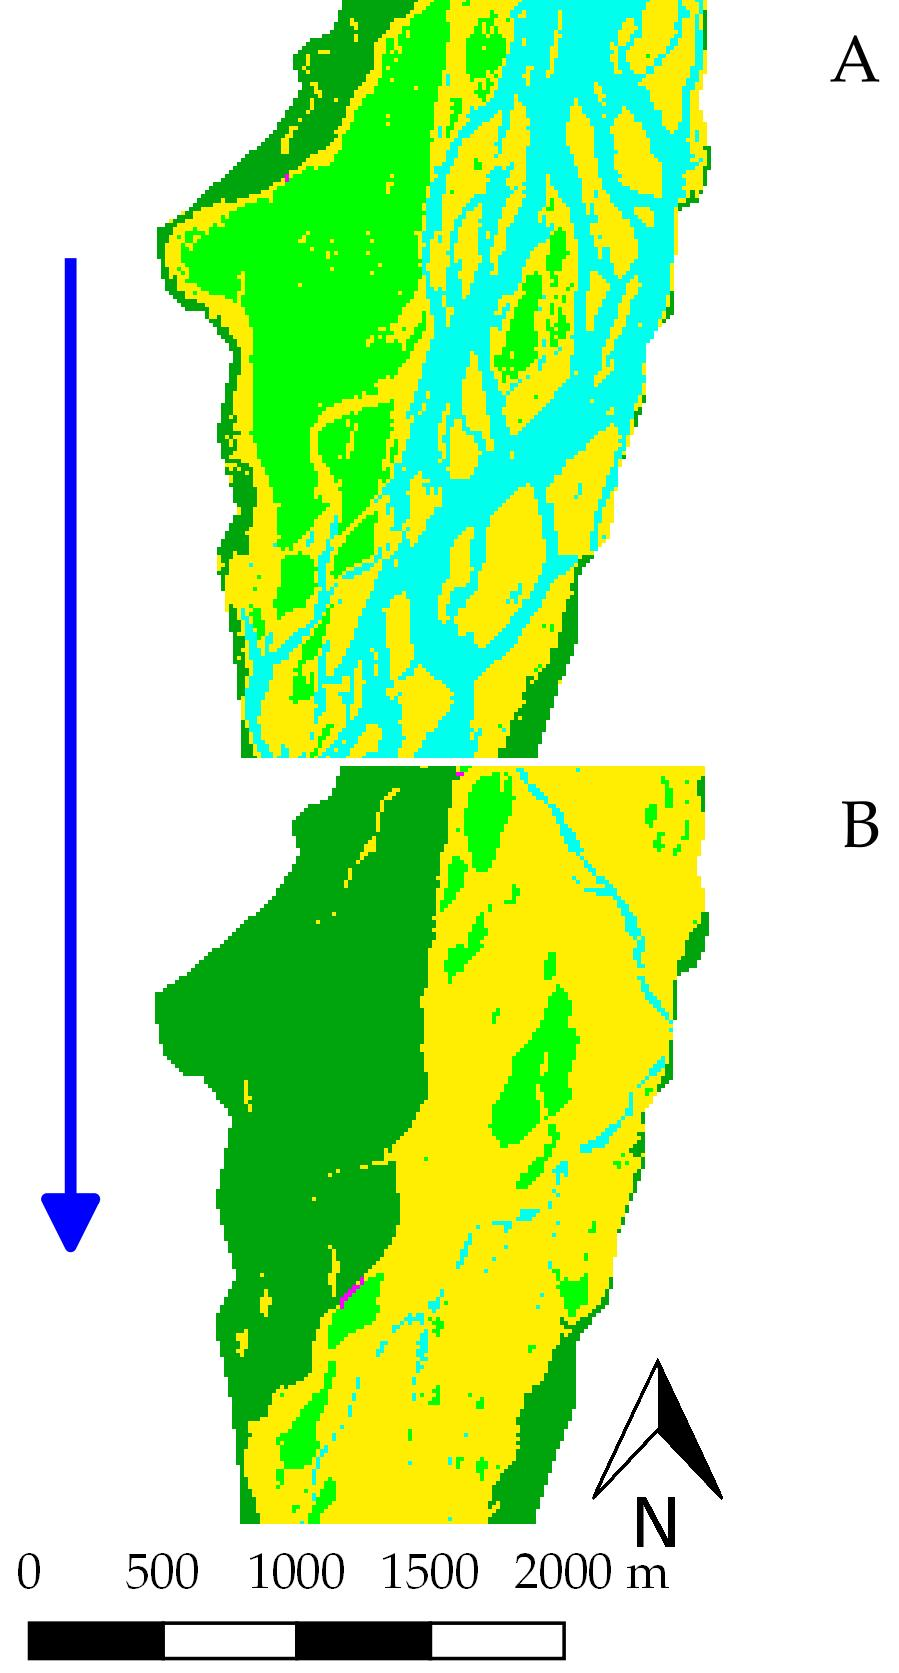
\includegraphics[width=0.3\textwidth]{files/fusione_isola_tr_15.jpeg}
	\caption[andamento temporale di $B$ per i tratti~7 e~15]{a sinistra si vede l'andamento nel tempo della larghezza media dell'alveo attivo $B$ dei tratti~7 e~15; la $B$ del tratto~7 oscilla solamente di qualche decina di metri, mentre il tratto~15 riduce improvvisamente la sua $B$ a causa della fusione di una grande isola nella \emph{floodplain}, fenomeno mostrato a destra (A: 2002-06-12, B: 2005-08-30).}
	\label{fig:b-media-7-e-15}
\end{figure}
%

È interessante confrontare alcuni risultati con quanto è stato svolto da altri autori: \squarecites{Zanoni:2008}{Surian:2015} riportano per i tratti dal~6 al~12 (dal ponte autostradale di Braulins alla stretta di Pinzano) la larghezza media ottenuta tramite la classificazione manuale di ortofoto aeree del secolo scorso e del decennio passato e tramite documenti catastali del 1800; è dunque possibile osservare traiettorie evolutive molto estese (\cref{graph:larghezze-vs-letteratura}).
%
\begin{figure}
	\centering
	\tikzsetnextfilename{larghezze_vs_letteratura}
\begin{tikzpicture}
	\begin{groupplot}[
		group style = {
			group size = 2 by 1,
			ylabels at = edge left,
			x descriptions at = edge bottom,
			horizontal sep = 0.5cm,
			vertical sep = 0.1cm,
		},
		width = 0.48\textwidth,
		height = 0.5\textwidth,
		date coordinates in = x,
		date ZERO = 1800-01-01,
		xticklabel = {$\year$},
		xticklabel style = {
			rotate = 80,
			anchor = near xticklabel
		},
		ylabel = {Larghezza \si{[\m]}},
		grid = major,
		]
		\nextgroupplot[
				legend columns = -1,
				legend to name = legend_larghezze,
				xtick distance = 18270,
			] % overview
			\addplot[green!70!black, mark = square*] % zanoni 2008
	        	table [x = data, y = larghezza] {graphics/data/largh_zanoni.txt};
	        	\addlegendentry{Zanoni et al. 2008}
			\addplot[orange, mark = triangle*] % surian 2015
	        	table [x = data, y = larghezza] {graphics/data/largh_surian.txt};
	        	\addlegendentry{Surian et al. 2015}
			\addplot[blue, mark = *] % mie
	        	table [x = data, y = larghezza] {graphics/data/largh_mie.txt};
	        	\addlegendentry{Presente tesi}
	        \draw [black, dashed, very thick] (1990-01-01,500) rectangle (2019-01-01,750);
	    %
		\nextgroupplot[
			xmin = 1990-01-01,
			ymin = 500,
			ymax = 750,
			yticklabel pos = right,
			xtick distance = 1827,
		] % zoom
			\addplot[green!70!black, mark = square*] % zanoni 2008
	        	table [x = data, y = larghezza] {graphics/data/largh_zanoni.txt};
			\addplot[orange, mark = triangle*] % surian 2015
	        	table [x = data, y = larghezza] {graphics/data/largh_surian.txt};
			\addplot[blue, mark = *] % mie
	        	table [x = data, y = larghezza] {graphics/data/largh_mie.txt};
	        \node [fill = white, draw = black, dashed, anchor = south east] 
        	at (axis description cs: 1,0) {Ingrandimento};
	\end{groupplot}
	%
	\draw [thick, blue, ->, shorten > = 2pt, shorten < = 2pt]
		(group c1r1.east) -- (group c2r1.west);
    %\node at ($(group c1r1) + (3.5cm,3.3cm)$) {\pgfplotslegendfromname{legend_larghezze}};
    \node at (group c1r1.north east) [anchor=south, xshift=.4cm] %.4cm è la metà della distanza orizzontale tra i plot
    	{\pgfplotslegendfromname{legend_larghezze}};
\end{tikzpicture}
	\caption[traiettoria evolutiva della larghezza media dell'area compresa tra il tratto~6 e il tratto~12]{traiettoria evolutiva della larghezza media dell'area compresa tra il tratto~6 e il tratto~12; sono presenti le traiettorie ottenute da \squarecite{Zanoni:2008} e da \squarecite{Surian:2015}.}
	\label{graph:larghezze-vs-letteratura}
\end{figure}
%
\\
Si vede chiaramente come i tratti si siano ristretti nel corso degli ultimi due secoli, forse a causa di lievi cambiamenti naturali nel regime idrologico, ma molto più probabilmente per le attività umane di prelievo di legname ed estrazione della ghiaia dall'alveo, avvenuti con particolare intensità nella seconda metà del 1900, così come degli interventi di ingegneria fluviale attuati dal 1950 (argini, soglie e opere di presa).
\\
In seguito, la concomitanza di piene importanti, della messa al bando dell'estrazione di ghiaia di fiume e della cessazione dell'utilizzo del legno presente in alveo per un cambiamento culturale ha indotto un graduale riallargamento di qualche centinaio di metri.
\\
I risultati in letteratura sono generalmente in accordo tra loro, così come non si discostano dai risultati della presente tesi.
Questi ultimi mostrano delle oscillazioni tra lievi allargamenti e restringimenti; sembra comunque che, anche negli ultimi \SI{20}{\anni} circa, questo tratto di fiume si stia ancora allargando, anche se ad un tasso sicuramente inferiore rispetto al decennio precedente.
Osservando proprio gli ultimi punti, si può quasi leggere un leggero restringimento; questo potrebbe essere reale, così come dovuto agli errori nella classificazione, data la modesta entità del cambiamento.
\\
Si nota una certa differenza tra le tre curve: alcuni punti degli altri lavori, punti che chiaramente provengono dalla classificazione delle medesime immagini, hanno valori di larghezza che differiscono di diverse decine di metri.
Questo può dipendere dal metodo di digitalizzazione dell'alveo e dalla definizione di isole, in particolare di quelle originatesi dal distacco di parte di piana alluvionale o di quelle in procinto di fondersi nella stessa.
Tuttavia, è la traiettoria evolutiva ciò che è importante evincere da questi risultati.

\section{Risultati e discussione: percentuale di isole in alveo}
Grazie alle mappe di classificazione dell'alveo è possibile ottenere informazioni riguardo la quantità di isole presenti nei tratti rispetto all'alveo attivo.
Questa proporzione è utile per delineare zone in cui la vegetazione riesce a prosperare, o per individuare momenti in cui le isole si sono espanse, così come per verificare come la connessione con la falda nel materasso alluvionale influenzi la crescita delle piante.
\\
Il grafico in \cref{graph:rapp-isl-tutti-tratti} mostra il rapporto tra l'area delle isole presenti in ogni tratto valido in ogni immagine e il relativo areale di alveo attivo.
La sua lettura è analoga al grafico in \cref{graph:larghezze-tutti-tratti}: le “strisce” verticali sono delle fotografie di un preciso momento in cui l'alveo presentava quella specifica proporzione di isole; le “strisce” orizzontali sono le traiettorie evolutive dei singoli tratti.
%
\begin{figure}
	\centering
	\tikzsetnextfilename{rapp_isl_tutti_tratti}
\begin{tikzpicture}
	\begin{axis}[
		width = \textwidth,
		height = \textwidth,
		symbolic x coords = {2000-09-17, 2001-06-07, 2002-05-18, 2002-06-12, 2003-06-22, 2004-10-14, 2005-08-30, 2006-07-16, 2007-09-21, 2008-07-05, 2009-07-08, 2010-09-29, 2011-10-02, 2012-08-01, 2013-09-05, 2014-09-08, 2014-10-31, 2015-08-13, 2015-09-12, 2015-10-22, 2016-09-13, 2017-04-21, 2017-06-13, 2018-06-15, 2018-09-16},
		xticklabel style = {
			rotate = 90,
		},
		xtick distance = 1,
		ymin = 1,
		ymax = 23,
		ytick = data,
		ylabel = {Tratto},
		y dir = reverse,
		enlargelimits = 0.02,
		colorbar horizontal,
		colorbar style = {
			xlabel = {Proporzione di isole sull'alveo attivo},
			xticklabel style = {
				/pgf/number format/.cd,
				fixed,
				fixed zerofill,
				precision = 2,
				/tikz/.cd,
			},
			xtick distance = 0.04,
		},
		]
		\addplot[
			matrix plot*,
			mesh/cols = 23,	% per fargli leggere colonne formate da 23 righe dal file di testo
			shader = flat corner,	% per interpolare i colori
		]
        	table [y = tratto, x = data, point meta = \thisrow{rapp_isl}] {graphics/data/rapp_isl_tutti_tratti.txt};
	\end{axis}
\end{tikzpicture}

	\caption[rapporto delle isole sull'alveo attivo in ogni tratto per ogni immagine]{rapporto delle isole sull'alveo attivo in ogni tratto per ogni immagine; i quadrati bianchi indicano assenza di dati (a causa della presenza di nuvole o limitata estensione dell'immagine); è stato escluso il tratto~9, che contiene l'isola di Cornino che si fonda su roccia e non è soggetta alle stesse dinamiche delle altre isole.}
	\label{graph:rapp-isl-tutti-tratti}
\end{figure}
%
\\
Da monte verso valle, si vede come alcuni tratti siano più adatti di altri ad ospitare delle isole, come i tratti dal~7 all'11 o quelli planiziali;
i tratti montani e quelli più vallivi sono i meno vegetati, sicuramente poiché sono stretti e il disturbo indotto dalle piene è frequente ed intenso.
È da ricordare che nel tratto~9 è presente l'isola di Cornino, che a differenza delle altre isole si fonda su roccia anziché su ghiaia.
\\
Si osserva inoltre l'effetto della risalita e dello sprofondamento della falda:
i tratti con \emph{upwelling}, come quelli tra il~7 e l'11 e quelli tra il~19 e il~22, sono quelli che possono essere colonizzati da molte isole se le altre condizioni ambientali sono favorevoli; i tratti con \emph{downwelling} sono invece generalmente meno vegetati, a meno di grandi isole che si sono in seguito fuse con le sponde. Queste isole si sono formate negli ultimi due decenni del 1900, quando le condizioni erano molto probabilmente favorevoli per la crescita, l'espansione e la coalescenza di più isole.
Questi trend spaziali sono mostrati nel grafico in \cref{graph:rapp-isl-2008-2016}.
%
\begin{figure}
	\centering
	\tikzsetnextfilename{rapp_isl_2008_2016}
\begin{tikzpicture}
	\begin{axis}[
		width = \textwidth,
		height = 0.5\textwidth,
		xtick = data,
		enlarge x limits = 0.01,
		xlabel = {Tratto},
		ylabel = {Rapporto isole su alveo attivo},
		grid = major,
		legend style = {
			at = {(0,1)},
			anchor = north west,		
		},
		]
		\addplot[
			violet,
			mark = triangle,
			unbounded coords = jump,
			]
        	table [x = tratto, y = rapp_isl_2008,] {graphics/data/rapp_isl_2008_2016.txt};
        \addlegendentry{2008-07-05};
        	
		\addplot[
			cyan,
			mark = triangle,
			unbounded coords = jump,
			]
        	table [x = tratto, y = rapp_isl_2016,] {graphics/data/rapp_isl_2008_2016.txt};
        \addlegendentry{2016-09-13};
	\end{axis}
\end{tikzpicture}

	\caption[proporzione di isole sull'alveo attivo nel 2008-07-05 e nel 2016-09-13]{proporzione di isole sull'alveo attivo nell'immagine \AST{} 2008-07-05 e nell'immagine \Se{} 2016-09-13; si notano le zone più vegetate proprio nei tratti dove c'è \emph{upwelling} e quelle meno vegetate dove c'è \emph{downwelling}; non è rappresentato il tratto~9 poiché contiene l'isola di Cornino, che si fonda su roccia.}
	\label{graph:rapp-isl-2008-2016}
\end{figure}
%

Si è proceduto confrontando parte dei dati ottenuti con i risultati riportati in due lavori \squarecites{Zanoni:2008}{Surian:2015} (\cref{graph:rapp-isl-vs-letteratura}).
Non sono presenti dati antecedenti al 1940, come invece erano stati riportati per la larghezza, poiché gli autori non hanno considerato affidabili le mappe del catasto austriaco nel definire i limiti delle isole.
Questi risultati sono limitati ai tratti compresi tra il ponte autostradale presso Braulins (tratto~6) e la stretta di Pinzano (tratto~12).
%
\begin{figure}
	\centering
	\tikzsetnextfilename{rapp_isl_vs_letteratura}
\begin{tikzpicture}
	\begin{axis}[
		width = \textwidth,
		height = 0.5\textwidth,
		date coordinates in = x,
		date ZERO = 1940-01-01,
		xticklabel = {$\year$},
		xticklabel style = {
			rotate = 80,
			anchor = near xticklabel
		},
		xtick distance = 3660,
		enlarge x limits = 0.02,
		ylabel = {Rapporto isole su alveo attivo},
		grid = major,
		legend style = {
			anchor = north west,
			at = {(0,1)},
		},
		scaled ticks = false,
		%legend columns = -1,
		]
		\addplot[blue, mark = square*] % zanoni 2008
	        table [x = data, y = rapp_isl] {graphics/data/rapp_isl_zanoni.txt};
	        \addlegendentry{Zanoni et al. 2008}
	    \addplot[green!70!black, mark = triangle*] % surian 2015
	        table [x = data, y = rapp_isl] {graphics/data/rapp_isl_surian.txt};
	     	\addlegendentry{Surian et al. 2015}
		\addplot[red, mark = *] % mie
	       	table [x = data, y = rapp_isl] {graphics/data/rapp_isl_mie.txt};
	       	\addlegendentry{Tesi}
	\end{axis}
\end{tikzpicture}
	\caption[rapporto tra isole e alveo attivo nell'area compresa tra il tratto~6 e il tratto~12]{rapporto tra isole e alveo attivo nell'area compresa tra il tratto~6 e il tratto~12; sono presenti i dati provenienti da \squarecite{Zanoni:2008} e da \squarecite{Surian:2015}.}
	\label{graph:rapp-isl-vs-letteratura}
\end{figure}
%
\\
Da una parte \squarecite{Zanoni:2008} suggerisce che la percentuale di vegetazione in alveo oscilla attorno al valore di \SI{8}{\percent}, dall'altra \squarecite{Surian:2015} mostra che la traiettoria evolutiva è assai simile a quella della larghezza.
I risultati di questa tesi sembrano seguire i risultati di entrambi: ad un primo periodo di crescita del rapporto isole su alveo seguono oscillazioni continue attorno ad un valore compreso tra \numrange[range-phrase={ e }]{0.12}{0.13}.
\\
Si vede chiaramente come nello stesso anno il rapporto tra isole e alveo attivo mostrato dai tre lavori considerati presenti valori molto diversi, come nel~1954, nel~2000, nel~2005, nel~2009 e nel~2011.
I dati della tesi si discostano abbastanza rapidamente dai dati da letteratura, in particolare dagli anni 2005-2006 quando in un periodo privo di piene intense la vegetazione ha potuto prosperare.
\\
Queste discordanze sono con tutta probabilità dovute ai differenti metodi che ogni autore ha utilizzato per delimitare le isole e l'alveo attivo, così come le mappe utilizzate:
nelle ortofoto ad alta risoluzione (celle di dimensione di poche decine di centimetri) è spesso possibile riconoscere la chioma di ogni pianta, mentre nelle immagini satellitari si può solo distinguere le forme vegetate dall'alveo;
\squarecite{Surian:2015} ha considerato come isole solamente le piante che vi crescono, senza tenere conto delle zone parzialmente vegetate o poco vegetate che possono esservi all'interno, ed ha escluso le piante “intermedie” e “alte” dall'areale dell'alveo attivo;
la presente tesi ha invece incluso le isole nel definire l'alveo attivo e la risoluzione minore della maggior parte delle immagini (cioè la maggior dimensione delle celle) ha permesso di delineare le isole come zone compatte di vegetazione, che raramente presentavano nel mezzo celle classificate come alveo o come canale.
In quanto le immagini satellitari ad alta risoluzione \Pl{} e \WV{} mostrano le stesse differenze di percentuale di isole su alveo attivo rispetto alle digitalizzazioni manuali, si ritiene che siano le scelte durante la fase di mappatura la fonte principale di scostamento tra i dati presentati.
\\
Le diversità non permettono un confronto dei risultati al fine di evincere un trend temporale.
Dai risultati della tesi sembra comunque certo che nei tratti in questione (dal~6 al~12) l'alveo abbia subito un incremento nella percentuale di isole, ma generalmente non oltre il \SI{15}{\percent}.


\section{Risultati: l'effetto della potenza della corrente sulle isole}
Il grafico in \cref{graph:omega-perc-50} mostra la mediana temporale della potenza della corrente per ogni tratto; si rappresenta la mediana poiché la variazione di $\Omega$ nel tempo è trascurabile (pochi punti percentuali).
Questo grafico riflette sia le caratteristiche morfologiche (pendenza e larghezza) che idrologiche (percentuale di area drenante).
%
\begin{figure}
	\centering
	\tikzsetnextfilename{omega_perc_50}
\begin{tikzpicture}
	\begin{axis}[
		width = 0.95\textwidth,
		height = .5\textwidth,
		enlarge x limits = 0.01,
		%enlarge y limits = 0.01,
		xlabel = {Tratto},
		ylabel = {Potenza della corrente \si{[\newton\per\metre\tothe{4}]}},
		xtick = data,
		grid = major,
		yticklabel style = {
			/pgf/number format/fixed
		},
		]
		\addplot[only marks, mark = *]
        	table [x = tratto, y = omega,] {graphics/data/omega_perc_50.txt};
	\end{axis}
\end{tikzpicture}
	\caption[potenza della corrente in ogni tratto]{mediana temporale su tutte le immagini della potenza della corrente pesata con la relativa area drenante mostrata per ogni tratto.}
	\label{graph:omega-perc-50}
\end{figure}
%
\\
È possibile osservare come i tratti più a monte abbiano una \emph{stream power} elevata grazie alla forte pendenza e alla ridotta larghezza; a monte del tratto~3 confluisce il Fella, il maggiore affluente del Tagliamento, e il suo contributo in termini di area drenante è evidente.
Più a valle, dove l'alveo si allarga a la pendenza diminuisce, $\Omega$ cala; tuttavia a monte e a valle della stretta di Pinzano (tratti~12 e~13, rispettivamente) il brusco restringimento incrementa la potenza della corrente.
Nei tratti planiziali $\Omega$ non varia particolarmente, mentre nell'ultimo tratto, dove la morfologia diventa di tipo transizionale e l'alveo si restringe sensibilmente, il valore di $\Omega$ quasi triplica.

Rappresentando la potenza della corrente rispetto alla proporzione di isole sull'alveo attivo, si vede un andamento iperbolico: utilizzando per entrambi gli assi una scala logaritmica (\cref{graph:omega-area-percentuale}), è possibile osservare l'effetto di controllo sulla quantità massima di vegetazione esercitato da $\Omega$.
\\
Da queste analisi è stato escluso il tratto~9, dove è presente l'isola di Cornino, poiché quest'isola è fondata su roccia e non è soggetta alle stesse dinamiche delle altre isole.
%
\begin{figure}
	\centering
	\tikzsetnextfilename{omega_area_percentuale_linear}
\begin{tikzpicture}
	\begin{axis}[
		width = \textwidth,
		height = .7\textwidth,
		enlarge x limits = 0.01,
		%enlarge y limits = 0.01,
		ylabel = {$\Omega$ \si{[\newton\per\metre\tothe{4}]}},
		xlabel = {Isole rispetto all'alveo attivo},
		xtick distance = 0.04,
		grid = major,
		legend columns = -1,
		legend style = {
			anchor = south,
			at = {(0.5, 1.01)},
		},
		ticklabel style = {
			/pgf/number format/.cd,fixed,
		},
		]
		\foreach \tratto in {1,2,...,23}
			{
			\addplot[
				only marks,
				forget plot,
			]
				table [y = om_tr_\tratto, x = area_tr_\tratto]
				{graphics/data/omega_area_percentuale.txt};
			}
		
%		\addplot [color = green, % T1
%			 line width = 2 pt,
%			 domain = 1e-3:4e-1,
%			 samples = 10,
%			 ] 
%			 {10^(-1.5184 - 0.1838 * log10(x))};
%		\addlegendentry{Fit 1}
%%		\node [fill = white, draw = green, anchor = east] % T1 
%%        	at (axis description cs: 1,0.6) {$y = 10^{-1.5184} \, x^{- 0.1838}$};
%        	
%		\addplot [color = orange, % T2
%			 line width = 2 pt,
%			 domain = 1e-3:4e-1,
%			 samples = 10,
%			 ]
%			 {10^(-1.5056 - 0.2516 * log10(x))};
%		\addlegendentry{Fit 2}
%%		\node [fill = white, draw = orange, anchor = east] % T2 
%%        	at (axis description cs: 1,0.75) {$y = 10^{-1.5056} \, x^{- 0.2516}$};
%        	
%		\addplot [color = cyan, % T3
%			 line width = 2 pt,
%			 domain = 1e-3:4e-1,
%			 samples = 10,
%			 ]
%			 {10^(-1.4085 - 0.2371 * log10(x))};
%		\addlegendentry{Fit 3}
%		\node [fill = white, draw = cyan, anchor = east] % T3 
%        	at (axis description cs: 1,0.9) {$y = 10^{-1.4085} \, x^{- 0.2371}$};
%        
%		\node [fill = white, draw = black, anchor = south west] % T3 
%        	at (axis description cs: 0,0) {$R^2 \in [0.3, 0.6]$ $P_\mathrm{val} < 0.0001$};
	\end{axis}
\end{tikzpicture}
	\caption[potenza della corrente rispetto alla proporzione di isole sull'alveo attivo, grafico lineare]{potenza della corrente rispetto alla proporzione di isole sull'alveo attivo; la scala degli assi è lineare.}
	\label{graph:omega-area-percentuale-linear}
\end{figure}
%
\begin{figure}
	\centering
	\tikzsetnextfilename{omega_area_percentuale}
\begin{tikzpicture}
	\begin{axis}[
		width = \textwidth,
		height = .5\textwidth,
		%enlarge x limits = 0.01,
		%enlarge y limits = 0.01,
		ylabel = {$\Omega$ \si{[\newton\per\metre\tothe{4}]}},
		xlabel = {Isole rispetto all'alveo attivo},
		grid = major,
		legend columns = -1,
		legend style = {
			anchor = south,
			at = {(0.5, 1.01)},
		},
		colormap = {fitting point colormap}{
				color = (black)
				color = (white!80!black)
%				color = (cyan!75!black)
%				color = (orange!75!black)
%				color = (green!75!black)
            },
        log ticks with fixed point,
        xmode = log,
        ymode = log,
        log basis x = 10,
        log basis y = 10,
		]
		\foreach \tratto in {1,2,...,23}
			{
			\addplot[
				scatter,
				only marks,
				point meta = {ifthenelse(y < -1.5184-0.1838*x, 1, ifthenelse(y < -1.5056 - 0.2516 * x, 0.7, 0))},
				point meta max = 1,
				point meta min = 0,
				forget plot,
			]
				table [y = om_tr_\tratto, x = area_tr_\tratto]
				{graphics/data/omega_area_percentuale.txt};
			}
		
		\addplot [color = green, % T1
			 line width = 2 pt,
			 domain = 1e-3:4e-1,
			 samples = 10,
			 ] 
			 {10^(-1.5184 - 0.1838 * log10(x))};
		\addlegendentry{Fit 1}
%		\node [fill = white, draw = green, anchor = east] % T1 
%        	at (axis description cs: 1,0.6) {$y = 10^{-1.5184} \, x^{- 0.1838}$};
        	
		\addplot [color = orange, % T2
			 line width = 2 pt,
			 domain = 1e-3:4e-1,
			 samples = 10,
			 ]
			 {10^(-1.5056 - 0.2516 * log10(x))};
		\addlegendentry{Fit 2}
%		\node [fill = white, draw = orange, anchor = east] % T2 
%        	at (axis description cs: 1,0.75) {$y = 10^{-1.5056} \, x^{- 0.2516}$};
        	
		\addplot [color = cyan, % T3
			 line width = 2 pt,
			 domain = 1e-3:4e-1,
			 samples = 10,
			 ]
			 {10^(-1.4085 - 0.2371 * log10(x))};
		\addlegendentry{Fit 3}
		\node [fill = white, draw = cyan, anchor = east] % T3 
        	at (axis description cs: 1,0.9) {$y = 10^{-1.4085} \, x^{- 0.2371}$};
        
		\node [fill = white, draw = black, anchor = south west] % T3 
        	at (axis description cs: 0,0) {$R^2 \in [0.3, 0.6]$ $P_\mathrm{val} < 0.0001$};
	\end{axis}
\end{tikzpicture}
	\caption[potenza della corrente rispetto alla proporzione di isole sull'alveo attivo, grafici bilogaritmico]{potenza della corrente rispetto alla proporzione di isole sull'alveo attivo con rette di regressione; nel grafico in alto ogni fit successivo considera solo i punti posti al di sopra del fit precedente; in quello in basso sono state utilizzate solo le massime percentuali di isole di ogni tratto nelle regressioni lineari; la scala di entrambi gli assi è logaritmica in base~\num{10}.}
	\label{graph:omega-area-percentuale}
\end{figure}
%
%\begin{figure}
%	\centering
%	\tikzsetnextfilename{omega_area_pura}
\begin{tikzpicture}
	\begin{axis}[
		width = \textwidth,
		height = .5\textwidth,
		%enlarge x limits = 0.01,
		%enlarge y limits = 0.01,
		ylabel = {$\Omega$ \si{[\newton\per\metre\tothe{4}]}},
		xlabel = {Isole rispetto all'alveo attivo \si{[\percent]}},
		xmode = log,
		ymode = log,
		grid = major,
		legend entries = {1,2,3,4,5,6,7,8,10,11,12,13,14,15,16,17,18,19,20,21,22,23},
		legend columns = 15,
		legend style = {
			anchor = south,
			at = {(0.5, 1.01)},
		},
		]
		\foreach \tratto in {1,2,...,23}
			{
			\addplot+[only marks]
				table [y = om_tr_\tratto, x = area_tr_\tratto]
				{graphics/data/omega_area_pura.txt};
			}
		
		\addplot [color = green, % T1
			 line width = 2 pt,
			 domain = 1e3:1e6,
			 samples = 10,
			 ] 
			 {10^(-0.3741 - 0.1820 * log10(x))};
		\node [fill = white, draw = cyan, anchor = east] % T1 
        	at (axis description cs: 1,0.9) {$10^{-0.3741} \, x^{- 0.1820}$};
        	
		\addplot [color = orange, % T2
			 line width = 2 pt,
			 domain = 1e3:1e6,
			 samples = 10,
			 ]
			 {10^(-0.0157 - 0.2366 * log10(x))};
		\node [fill = white, draw = orange, anchor = east] % T2 
        	at (axis description cs: 1,0.75) {$10^{-0.0157} \, x^{- 0.2366}$};
        	
		\addplot [color = cyan, % T3
			 line width = 2 pt,
			 domain = 1e3:1e6,
			 samples = 10,
			 ]
			 {10^(0.1130 - 0.2507 * log10(x))};
		\node [fill = white, draw = green, anchor = east] % T3 
        	at (axis description cs: 1,0.6) {$10^{0.1130} \, x^{- 0.2507}$};
        	
        \node [fill = white, draw = black, anchor = south west] % T3 
        	at (axis description cs: 0,0) {$R^2 \in [0.4, 0.8]$ $P_\mathrm{val} < 0.0001$};
	\end{axis}
\end{tikzpicture}
%	\caption[potenza della corrente rispetto all'areale delle isole]{potenza della corrente rispetto all'areale delle isole.}
%	\label{graph:omega-area-pura}
%\end{figure}
%
\\
Per ottenere relazioni che indichino quale sia il limite massimo di isole, sono state fatte due distinte regressioni lineari.
\\
Nella prima si è proceduto tramite regressioni lineari in successione: da una prima regressione su tutti i punti si sono selezionati solo i punti al di sopra della retta; si è eseguita una nuova regressione; con i punti posti superiormente alla seconda retta, si è ottenuta la retta finale di regressione.
Questa terza retta mostra un $R^2 \simeq 0.6$ ed un $P_\mathrm{value}$ ottenuto tramite il test statistico di Pearson minore di \num{0.0001} (valori di $R^2$ quanto più vicini all'unità e maggiori di~\num{0} indicano una buona regressione lineare; valori di $P_\mathrm{value}$ inferiori a~\num{0.05} mostrano che la regressione è affidabile nel risultato, sia che $R^2$ sia prossimo ad~\num{1} o sia quasi nullo).
\\
Nella seconda regressione sono state approssimate le mediane su tutte le immagini di $\Omega$ di ogni tratto rispetto alle massime percentuali di isole di ogni tratto. Tenendo conto che si è escluso il tratto~9, si effettua la regressione su~22 punti: in ascissa è rappresentato il valore di percentuale massima di isole per ognuno dei~22 tratti rimanenti e in ordinata il valore di $\Omega$.
Questa regressione è caratterizzata da $R^2 = 0.74$ e da $P_\mathrm{val} < 0.0001$.
\\
Data la discreta bontà di queste regressioni, le si accetta come valide.

\section{Discussione: formalizzazione di un modello concettuale}
In letteratura sono stati proposti modelli concettuali che relazionano la potenza della corrente con la quantità di vegetazione e il tipo di forma vegetata presente:
a bassi livelli di $\Omega$, il disturbo indotto dalla corrente è modesto e si possono formare numerose isole sulle barre nude in alveo;
se la potenza della corrente, cioè il disturbo, è maggiore, si potranno formare meno isole e le forme fluviali rimarranno prevalentemente nude \squarecite{Gurnell:2014-plants-eng}.
\\
Difatti l'espansione maggiore della vegetazione e l'erosione minore hanno luogo dove il tasso di crescita della vegetazione è elevato e dove l'energia della corrente è ridotta \squarecite{Gurnell:2006-omega}.
\\
Inoltre le piante che crescono più rapidamente sembrano essere maggiormente flessibili \squarecite{Bertoldi:2011-ASTER}: la ricrescita vegetativa da tronchi vivi, la quale permette un rapido sviluppo, è proprio la caratteristica fondamentale delle piante che abitano questo ambiente, come già esposto nella sezione~\ref{sec:descr-area-studio}.
È dunque lecito supporre che proprio nei tratti dove si osserva una ridotta potenza della corrente si possa trovare un'elevata quantità di isole nella maggior parte del periodo di studio.

Le due regressioni ottenute ricalcano bene il profilo iperbolico che mostravano i punti quando posti in un grafico in scala lineare (\cref{graph:omega-area-percentuale-linear-modello}); il terzo fit si pone al di sopra dei punti per percentuali di isole superiori al~\SI{5}{\percent}, mentre si adatta poco ai punti nel caso di percentuali inferiori; la regressione sulle massime percentuali sembra avere un comportamento generalmente migliore.
%
\begin{figure}
	\centering
	\tikzsetnextfilename{omega_area_percentuale_linear_regressioni}
\begin{tikzpicture}
	\begin{axis}[
		width = 0.97\textwidth,
		height = 0.97\textwidth,
		enlarge x limits = 0.01,
		%enlarge y limits = 0.01,
		ylabel = {$\Omega$ \si{[\newton\per\metre\tothe{4}]}},
		xlabel = {Isole rispetto all'alveo attivo},
		xtick distance = 0.04,
		enlargelimits = 0.02,
		grid = major,
		legend columns = -1,
		legend style = {
			anchor = south,
			at = {(0.5, 1.01)},
		},
		ticklabel style = {
			/pgf/number format/.cd,fixed,
		},
		]
		\foreach \tratto in {1,2,...,23}
			{
			\addplot[
				only marks,
				forget plot,
			]
				table [y = om_tr_\tratto, x = area_tr_\tratto]
				{graphics/data/omega_area_percentuale.txt};
			}
		
		\addplot [color = cyan, % modello
			 line width = 2 pt,
			 samples at = {0.01,0.012,...,0.32},
			 %domain y = 0.5:0.125,
			 %samples = 10,
			 ] 
			 {10 ^ (-1.4085) * x ^ (-0.2371)};
		%\addlegendentry{Fit 3}
%		\node [fill = white, draw = green, anchor = east] % T1 
%        	at (axis description cs: 1,0.6) {$y = 10^{-1.5184} \, x^{- 0.1838}$};
		
		\addplot [color = red, % modello
			 line width = 2 pt,
			 samples at = {0.01,0.012,...,0.32},
			 %domain y = 0.5:0.125,
			 %samples = 10,
			 ] 
			 {10 ^ (-1.6806) * x ^ (-0.4476)};
		%\addlegendentry{Max}
	\end{axis}
\end{tikzpicture}
	\caption[relazioni iperboliche tra potenza della corrente e percentuale di isole]{relazioni iperboliche tra potenza della corrente e percentuale di isole; in rosso la regressione sulle massime percentuali di isole rispetto all'alveo attivo, in azzurro la regressione sul terzo gruppo di punti di cui al grafico in \cref{graph:omega-area-percentuale}; la scala degli assi è lineare.}
	\label{graph:omega-area-percentuale-linear-regressioni}
\end{figure}
%
\\
Si sceglie quindi quest'ultima come rappresentativa del limite superiore di isole che l'alveo può supportare data una potenza della corrente (cioè una pendenza, una larghezza e un'area drenante del bacino secondo la sua definizione).

In un precedente lavoro è stato definito un unico valore limite di \emph{stream power} oltre il quale le isole non riescono più ad insediarsi a causa dell'intenso disturbo \squarecite{Gurnell:2006-omega}.
Tuttavia, questo valore è stato calcolato utilizzando l'equazione \eqref{eq:area-portata-mosetti}; per quanto già esposto, si è preferito non utilizzare tale relazione.
\\
I grafici mostravano un andamento iperbolico, il quale regola la percentuale massima di isole che riesce a stabilirsi con una data potenza;
questo andamento sembra fermarsi superiormente, attorno ad un valore di $\Omega$ di~\SIrange[range-phrase={-}, range-units = single]{0.12}{0.13}{\newton\per\metre\tothe{4}}, oltre il quale non è più presente vegetazione.
Si vede inoltre che l'alveo non ospita percentuali di vegetazione superiori al \SIrange[range-phrase={-}, range-units = single]{30}{35}{\percent}.

La relazione ottenuta presenta un limite implicito: $\Omega$ non tiene conto della connessione con la falda, dell'\emph{upwelling} e del \emph{downwelling}, che influenzano notevolmente la crescita delle piante.
Anzi, è stato mostrato che le isole complesse sono confinate nei tratti dove la crescita delle piante da seme può essere sufficientemente rapida (\SIrange[range-phrase={-}, range-units = single]{1}{3}{\m} in \SI{10}{\anni}; si ricorda che tramite la riproduzione vegetativa la crescita è più rapida di un ordine di grandezza); questi tratti sono quelli relativamente più stretti, dove c'è disponibilità d'acqua durante i periodi di magra grazie alla falda non troppo profonda, come i tratti pochi chilometri a monte della stretta di Pinzano o quelli a monte della zona di cambiamento di morfologia fluviale \squarecite{Gurnell:2006-omega}.
Dall'altra parte, come gli autori osservano e come è verificato dai risultati appena mostrati, dove i tratti si restringono maggiormente la potenza della corrente è tanto grande che nemmeno l'incrementato tasso di crescita delle piante è tale da permettere alle isole di insediarsi prima di essere portate via.
Gli autori suggeriscono quindi l'esistenza di un equilibrio tra processi idrologici, piante riparie e sviluppo delle isole, che si concretizza nei seguenti aspetti (grafico in \cref{graph:omega-area-percentuale-linear-modello}).
%
\begin{itemize}
	\item un valore massimo di $\Omega$ pari a \SIrange[range-phrase={-}]{0.12}{0.13}{\newton\per\metre\tothe{4}}, oltre il quale non sono presenti isole;
	\item un range di $\Omega$ in cui è possibile lo stabilirsi di isole, ma caratterizzato da un limite in cui il disturbo delle piene è predominante anche nelle zone relativamente più elevate dell'alveo;
	\item un limite massimo di isole, \numrange[range-phrase={-}]{0.30}{0.35}, che possono essere presenti anche con $\Omega$ molto bassi, in quanto l'insediamento di isole oltre queste limite avrebbe luogo sulle zone dell'alveo poste a quote relativamente minori, che sono le più disturbate dalle piene, mentre la zone situate a quote relativamente maggiori (creste delle barre, altre isole) sono tutte già vegetate.
\end{itemize}
%
%
\begin{figure}
	\centering
	\tikzsetnextfilename{omega_area_percentuale_linear_modello}
\begin{tikzpicture}
	\begin{axis}[
		width = \textwidth,
		height = .7\textwidth,
		enlarge x limits = 0.05,
		%enlarge y limits = 0.01,
		ylabel = {$\Omega$ \si{[\newton\per\metre\tothe{4}]}},
		xlabel = {Isole rispetto all'alveo attivo},
		xtick distance = 0.04,
		xmax = 0.44,
		grid = major,
		legend columns = -1,
		legend style = {
			anchor = south,
			at = {(0.5, 1.01)},
		},
		ticklabel style = {
			/pgf/number format/.cd,fixed,
		},
		]
		\foreach \tratto in {1,2,...,23}
			{
			\addplot[
				only marks,
				forget plot,
				gray,
			]
				table [y = om_tr_\tratto, x = area_tr_\tratto]
				{graphics/data/omega_area_percentuale.txt};
			}
		
		\addplot [color = purple, % limite superiore
			 line width = 2 pt,
			 ] 
			 coordinates {(-0.01,0.13) (0.02,0.13)};
		\node [fill = white, draw = purple, anchor = west] 
        	at (0.04,0.13) {$\Omega_\mathrm{max} \simeq\SI{0.13}{\newton\per\metre\tothe{4}}$};
		
		\addplot [color = red, % iperbole
			 line width = 2 pt,
			 samples at = {0.018,0.019,...,0.325},
			 ] 
			 {10 ^ (-1.6806) * x ^ (-0.4476)};
		\node [fill = white, draw = red, anchor = south west] 
        	at (0.08,0.08) {$y = 0.021 \, x ^ {-0.4476}$};
		
		\addplot [color = teal, % limite superiore
			 line width = 2 pt,
			 dashed,
			 ] 
			 coordinates {(0.35,0.02) (0.35,0.035)};
		\node [fill = white, draw = teal, anchor = east] 
        	at (0.42,0.06) {Proporzione max di isole $\simeq \num{0.35}$};
	\end{axis}
\end{tikzpicture}
	\caption[modello che lega la potenza della corrente con la percentuale massima di isole]{modello che lega la potenza della corrente $\Omega$ con la percentuale massima di isole; sono individuati in rosso scuro il limite di $\Omega$ oltre il quale non sono presenti isole, in rosso la relazione iperbolica tra $\Omega$ e il massimo di proporzione di isole osservato in ogni tratto, in verde-blu il massimo rapporto di isole rispetto all'alveo attivo osservato.}
	\label{graph:omega-area-percentuale-linear-modello}
\end{figure}
%

%----------------------------------------------------------



\chapter{In quali condizioni e in quale misura le isole variano?}
\bigskip
\section{Metodi: ottenere mappe che mostrano il cambiamento}
\label{sec:cambiamento}
A partire dalle mappe di classificazione dell'alveo, si sono ottenute mappe che mostrano come le isole sono, o non sono, cambiate: sono stati osservati infatti fenomeni di erosione, crescita, fusione nella \emph{floodplain} o permanenza (nessun cambiamento).
\\
Per ottenere questi dati, ogni mappa è stata confrontata con quella temporalmente precedente.
\\
L'analisi si è focalizzata sulle isole, mentre si è esclusa la piana alluvionale.

\subsection{Approccio}
\label{subsec:camb-approccio}
Alcune mappe hanno una estensione limitata oppure presentano zone con copertura nuvolosa: ciò riduce il numero di confronti possibili per alcuni tratti. 
Dalle 23 immagini satellitari (si veda la \cref{tab:date-orto-sat}) si sono ottenute in media 20~immagini di confronto per tratto.

Inoltre, le immagini \AST{} non sono correttamente georeferenziate e non sono perfettamente sovrapponibili; l'entità di questo scostamento è dell'ordine di qualche cella.
Questo difetto è di grande importanza poiché per poter investigare l'evoluzione temporale delle isole occorre poter osservare nel tempo ogni cella; se questa si sposta da un'immagine alla successiva, il confronto non è più valido.
\\
La soluzione adottata è stata quella di traslare ogni mappa a nord, sud, est o ovest del numero di celle necessario per poterla sovrapporre alla mappa temporalmente precedente.
L'operazione è stata ripetuta per ogni confronto, per ogni tratto, ed è stata verificata visivamente.
Il massimo errore residuo è di 1~cella (\SI{15}{\m}) di scostamento in pochissime zone nei primi tratti (\numrange[range-phrase={ - }]{1}{4}); data la locale topografia montuosa si è preferito ridurre l'errore a tale entità e tenerlo sotto controllo piuttosto di distorcere la mappa con altre misure di georettifica.
L'entità di questo errore è accettabile poiché quasi tutte le isole hanno estensione maggiore di \SI{225}{\m\tothe{2}}.
\\
Le altre immagini sono invece correttamente georeferenziate.

Infine, per poter confrontare immagini a diversa dimensione di cella, come le \AST{} a~\SI{15}{\m} con le \Pl{} a~\SI{0.5}{\m}, è stato necessario ricampionare le immagini con la dimensione minore (ad esempio le \Pl{}) riportandole alla risoluzione di quelle a dimensione maggiore (le \AST{} o le \Se{}).
\\
Nel ricampionamento l'areale delle isole subisce un incremento o una riduzione, così come l'areale della ghiaia e delle altre classi in quanto nelle celle a dimensione maggiore sono presenti numerose celle a dimensione minore, ognuna con un valore diverso (\cref{fig:ricamp-explanation}).
%
\begin{figure}
	\centering
	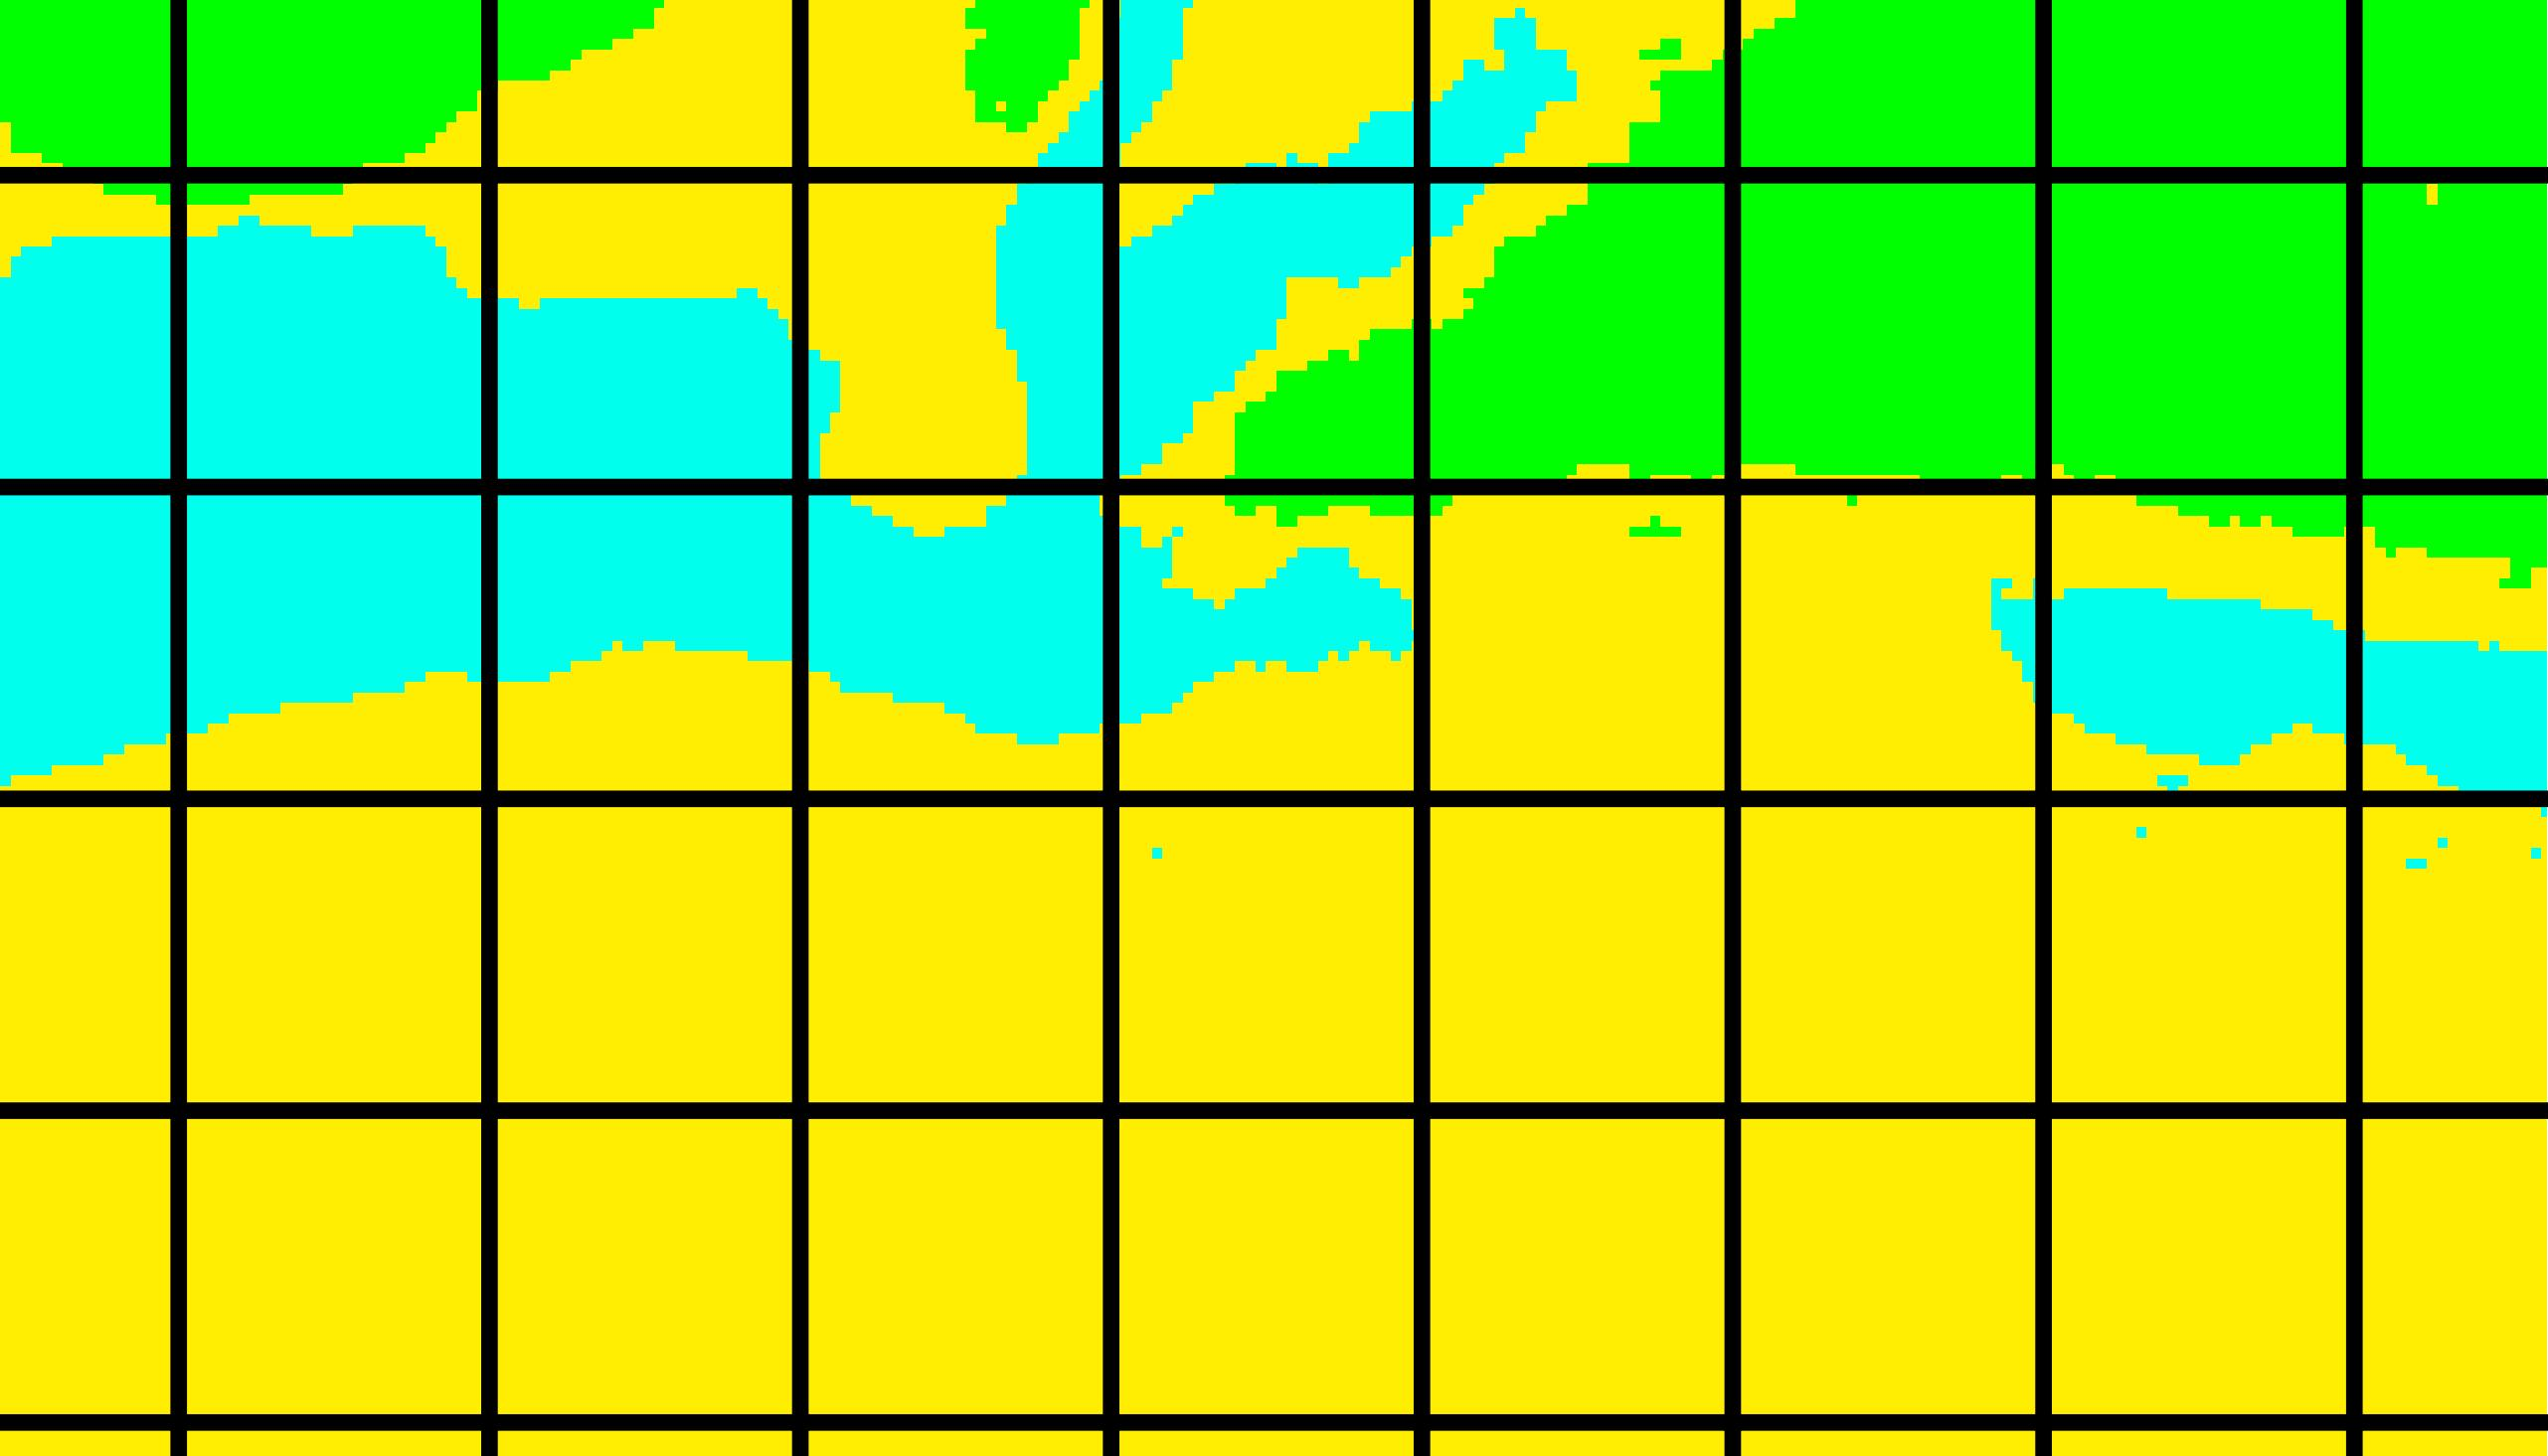
\includegraphics[width=.9\textwidth]{files/ricamp_griglia.jpeg}
	\caption[celle a risoluzione diversa]{immagine \Pl{} 2015-08-13 a~\SI{0.5}{\m} sullo sfondo, con la griglia a~\SI{15}{\m} in primo piano; si vede come diverse celle più piccole siano contenute in una singola cella maggiore.}
	\label{fig:ricamp-explanation}
\end{figure}
%
Nel ricampionamento si sceglie quale valore assegnare alla nuova cella più grande in base ai valori delle celle minori; nel presente lavoro si è scelto di assegnare un percentile.
La scelta del percentile è stata effettuata confrontando la radice quadrata della somma dei quadrati residui (RSQR):
%
\begin{equation}
	\label{eq:rad-som-quad-res}
	RSQR = \left\lbrace \sum_{n=1}^{cl} \left[\left( \frac{area_{\mathrm{orig,n}}}{area_{\mathrm{orig,tot}}} - \frac{area_{\mathrm{perc,n}}}{area_{\mathrm{perc,tot}}} \right)^2 \right] \right\rbrace ^ \frac{1}{2}	
\end{equation}
%
dove 
\begin{itemize}
	\item $cl$ è il numero di classi (\cref{tab:class-tratti});
	\item $n$ indica la $n$-esima classe;
	\item $area_{\mathrm{orig,n}}$ e $area_{\mathrm{perc,n}}$ sono l'area della $n$-esima classe rispettivamente nella mappa originale e in quella ricampionata al $perc$-esimo percentile;
	\item $area_{\mathrm{orig,tot}}$ e $area_{\mathrm{perc,tot}}$ sono l'area totale rispettivamente nella mappa originale e in quella ricampionata al $perc$-esimo percentile. 
\end{itemize} 
%
Si è scelto di normalizzare l'area di ogni classe usando come fattore di normalizzazione l'area totale per poter lavorare con percentuali.
\\
Nei ricampionamenti da \SI{0.5}{\m}, il $50_\mathrm{mo}$ percentile (mediana) è quello che mostra il minor RSQR ($<\SI{3}{\percent}$). Un esempio del risultato ottenuto è mostrato in \cref{fig:ricampionamento}.
%
\begin{figure}
	\centering
	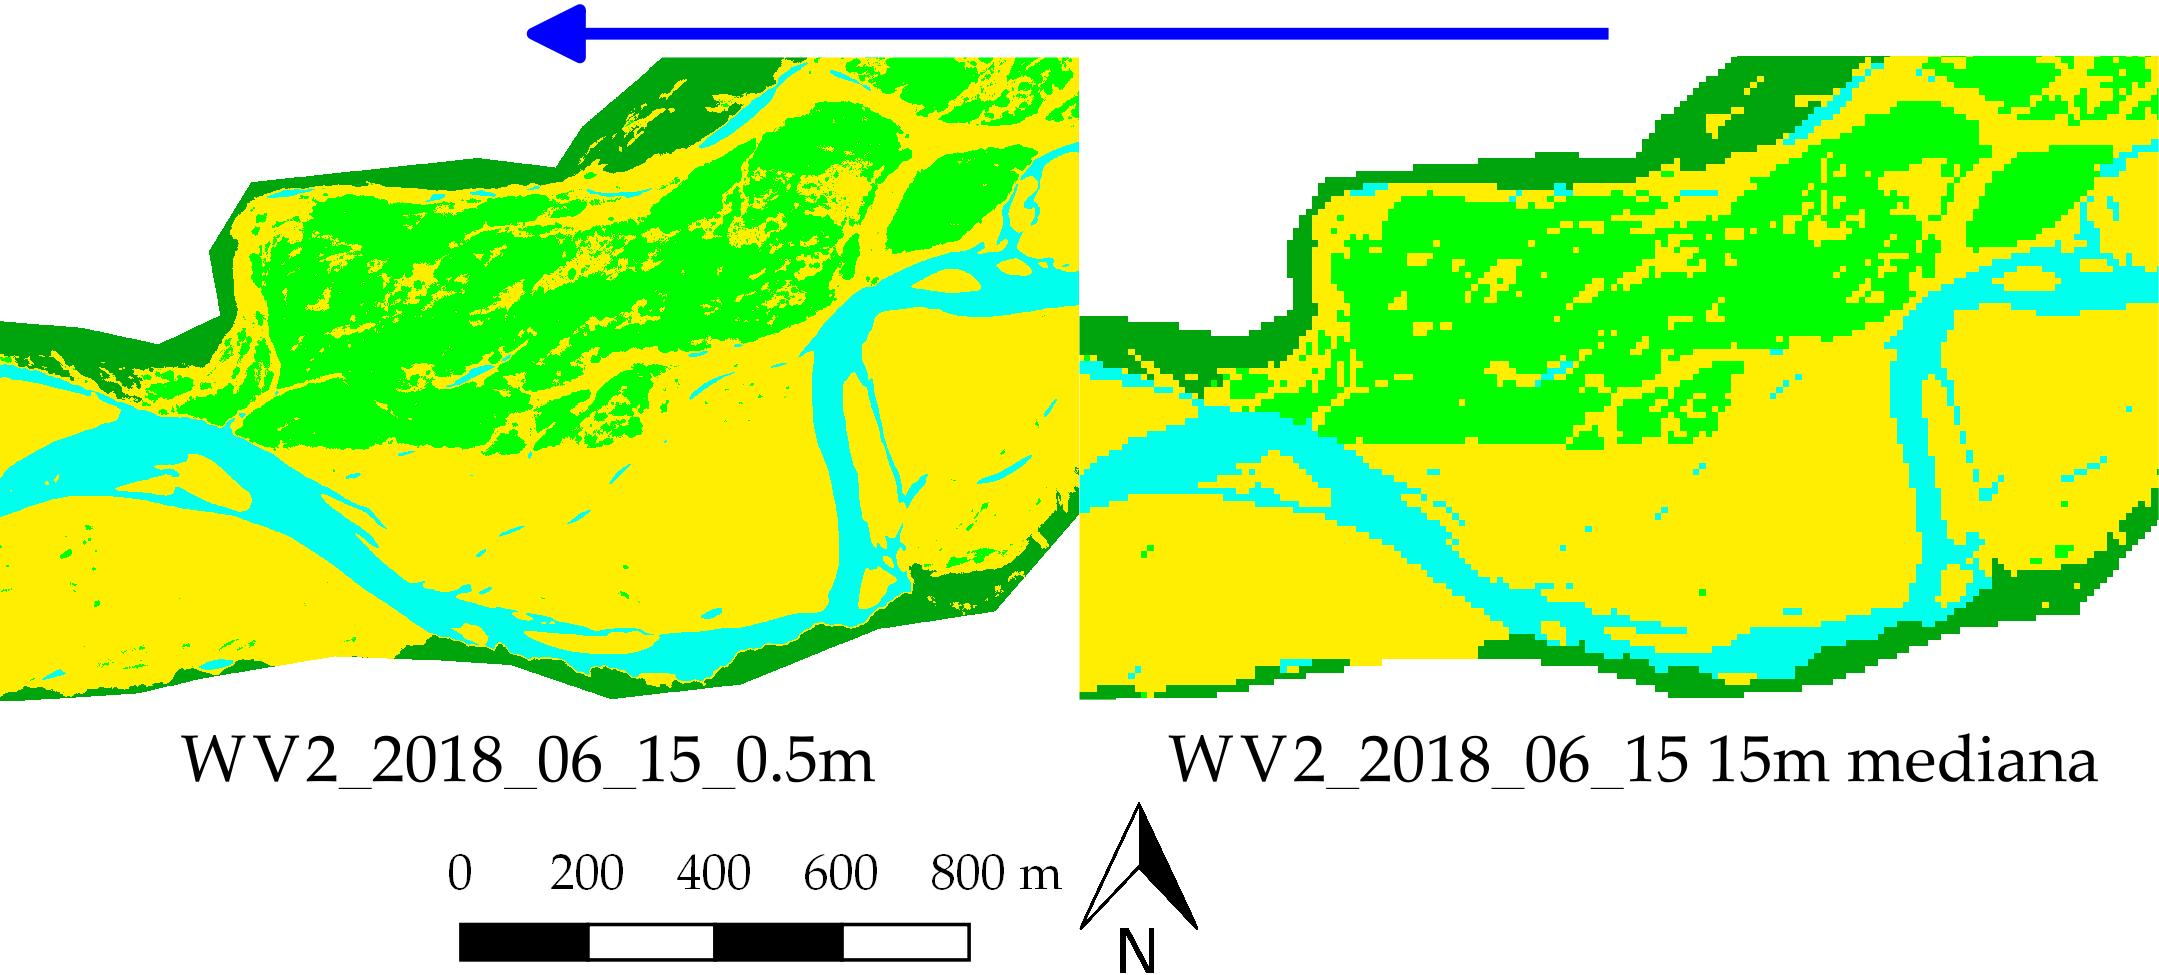
\includegraphics[width=\textwidth]{files/ricamp_class_is_fl.jpeg}
	\caption[confronto originale - ricampionamento]{a sinistra l'immagine \WV{} originale, poco a valle dell'isola di Cornino; a destra la stessa immagine ricampionata a~\SI{10}{\m} distribuendo i valori con la mediana.}
	\label{fig:ricampionamento}
\end{figure} 
%


\subsection{Confronti validi}
Dalle 23 immagini satellitari è stato possibile ottenere il numero di confronti mostrati in \cref{tab:confronti}. 
I confronti effettuati hanno la massima risoluzione temporale possibile, cioè per ogni tratto si sono confrontate le immagini valide temporalmente più vicine, in modo da poter osservare gli effetti cumulati del minor numero possibile di eventi di piena.
%
\begin{table}
	\centering
	\begin{tabular}{
		S[table-format=2.0] 
		S[table-format=2.0]@{\;}
		c 
		c}
		\toprule
		\textbf{Tratto}	&	\multicolumn{1}{c}{\textbf{Confronti}}	&	\textbf{Primo}		&	\textbf{Ultimo}	\\
						&	\multicolumn{1}{c}{\textbf{validi}}		&	\textbf{confronto}	&	\textbf{confronto}	\\
		\midrule
		1	&	17	&	2000-09-17/2002-05-18	&	2017-09-13/2018-09-16	\\
		2	&	18	&	2000-09-17/2002-05-18	&	2017-09-13/2018-09-16	\\
		3	&	19	&	2000-09-17/2001-06-07	&	2017-09-13/2018-09-16	\\
		4	&	19	&	2000-09-17/2001-06-07	&	2017-09-13/2018-09-16	\\
		5	&	19	&	2000-09-17/2001-06-07	&	2017-09-13/2018-09-16	\\
		6	&	23	&	2000-09-17/2001-06-07	&	2018-06-15/2018-09-16	\\
		7	&	23	&	2000-09-17/2001-06-07	&	2018-06-15/2018-09-16	\\
		8	&	23	&	2000-09-17/2001-06-07	&	2018-06-15/2018-09-16	\\
		9	&	22	&	2000-09-17/2002-05-18	&	2018-06-15/2018-09-16	\\
		10	&	22	&	2000-09-17/2002-05-18	&	2018-06-15/2018-09-16	\\
		11	&	21	&	2000-09-17/2002-05-18	&	2018-06-15/2018-09-16	\\
		12	&	21	&	2000-09-17/2002-05-18	&	2018-06-15/2018-09-16	\\
		13	&	22	&	2000-09-17/2002-05-18	&	2018-06-15/2018-09-16	\\
		14	&	23	&	2000-09-17/2002-05-18	&	2018-06-15/2018-09-16	\\
		15	&	19	&	2000-09-17/2002-06-12	&	2017-09-13/2018-09-16	\\
		16	&	19	&	2000-09-17/2002-06-12	&	2017-09-13/2018-09-16	\\
		17	&	19	&	2000-09-17/2002-06-12	&	2017-09-13/2018-09-16	\\
		18	&	19	&	2000-09-17/2002-06-12	&	2017-09-13/2018-09-16	\\
		19	&	19	&	2000-09-17/2002-06-12	&	2017-09-13/2018-09-16	\\
		20	&	19	&	2000-09-17/2002-06-12	&	2017-09-13/2018-09-16	\\
		21	&	19	&	2000-09-17/2001-06-07	&	2017-09-13/2018-09-16	\\
		22	&	19	&	2001-06-07/2002-06-12	&	2017-09-13/2018-09-16	\\
		23	&	19	&	2001-06-07/2002-06-12	&	2017-09-13/2018-09-16	\\
		\bottomrule
	\end{tabular}
	\caption[confronti effettuati]{confronti effettuati con le 23 immagini satellitari a disposizione per ottenere dati sul cambiamento delle isole.}
	\label{tab:confronti}
\end{table}
%

\subsection{Classi di cambiamento}
In ogni confronto ci si è concentrati sui fenomeni riguardanti l'evoluzione delle isole, individuandone~4 (si veda anche la \cref{tab:class-tratti}):
%
\begin{itemize}
	\item erosione (da isola ad alveo attivo);
	\item crescita (da alveo attivo ad isola);
	\item fusione nella \emph{floodplain} (da isola a \emph{floodplain});
	\item distaccamento dalla \emph{floodplain} (da \emph{floodplain} a isola);
	\item nessun cambiamento (da isola a isola).
\end{itemize}
%
Un esempio di questa classificazione è riportato nella \cref{fig:confr-class-is-fl}.
%
\begin{figure}
	\centering
	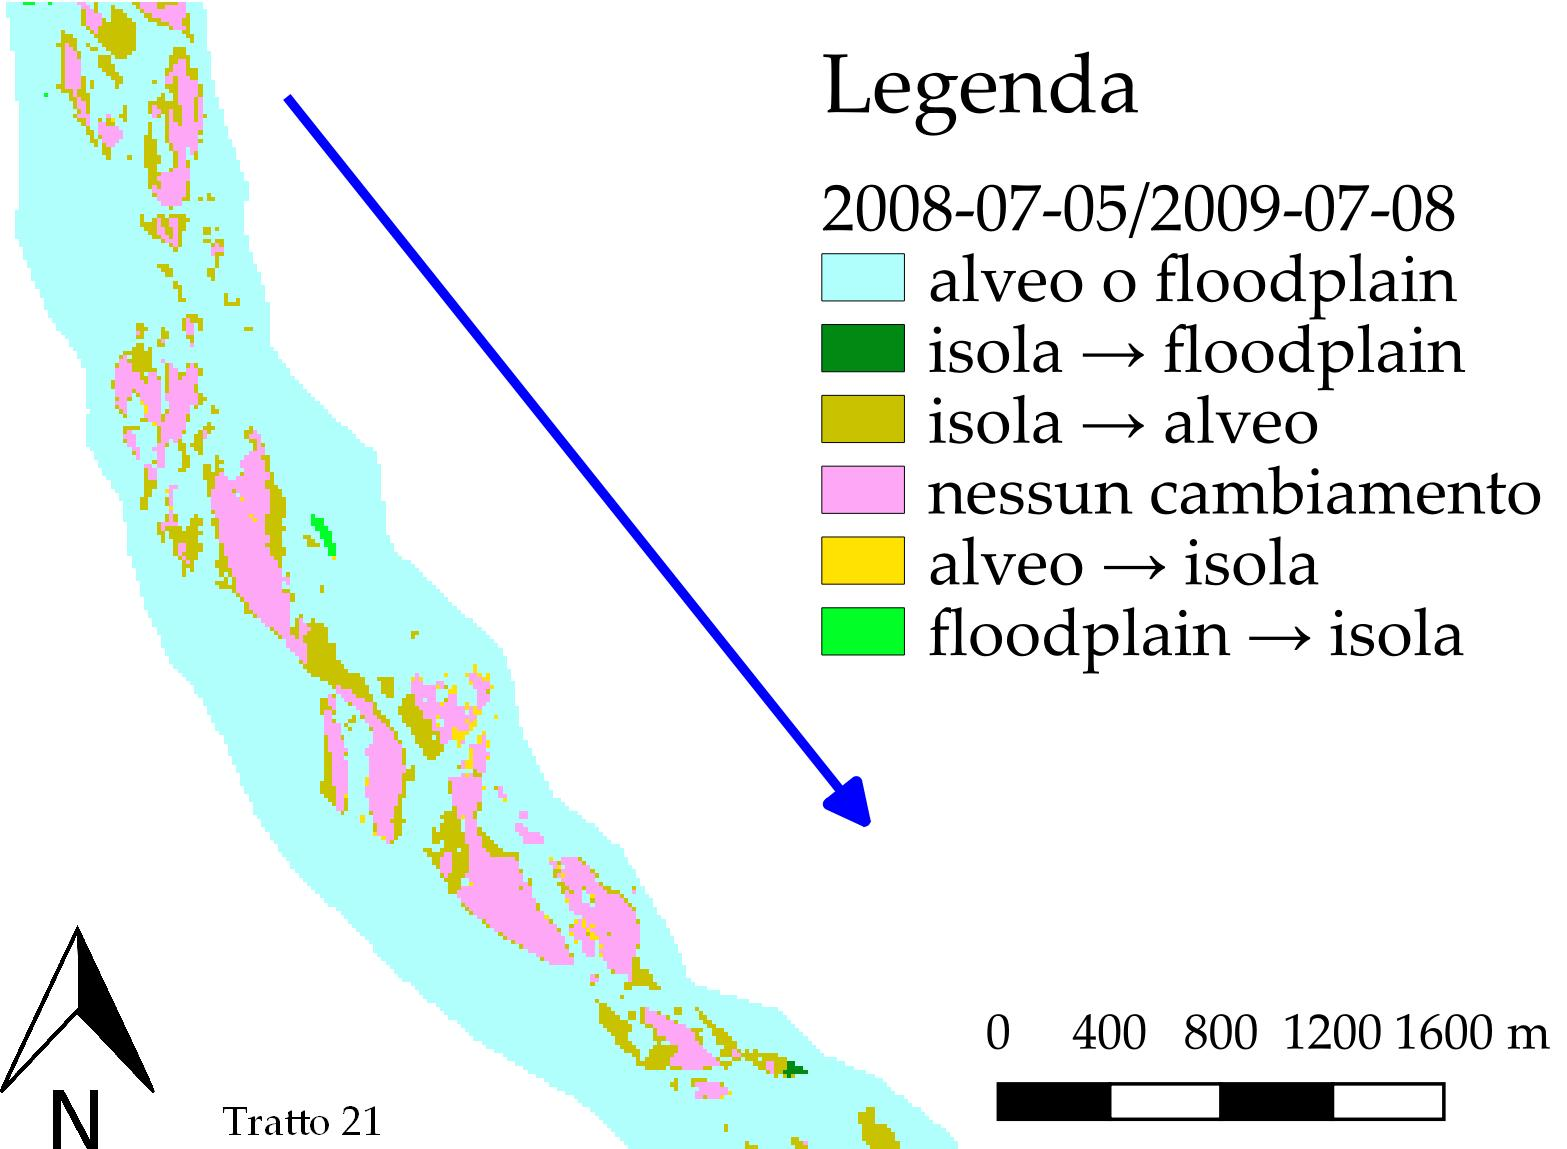
\includegraphics[width=.8\textwidth]{files/confr_class_is_fl.jpeg}
	\caption[esempio di mappa di cambiamento]{esempio di mappa di cambiamento ottenuta con il confronto tra le immagini \AST{} 2008-07-05 e 2009-07-08. Si possono osservare tutti i cambiamenti possibili; la prima classe, colorata in azzurro, visualizza l'area dell'intera maschera computazionale, e comprende perciò sia l'alveo che la \emph{floodplain}. Il tratto mostrato è posto qualche \si{\kilo\m} a monte del ponte di Madrisio.}
	\label{fig:confr-class-is-fl}
\end{figure}
%


\section{Metodi: mappare gli elementi legnosi in alveo}
Le piante che caratterizzano l'ambiente ripario nell'area di studio (\emph{Salix spp.} e \emph{Populus nigra}) sono in grado di riprodursi tramite la dispersione di semi;
tuttavia, la riproduzione vegetativa a partire da elementi legnosi, quali pezzi di tronchi, piante e arbusti e accumuli di legname, ottiene un successo maggiore e costituisce il fondamentale meccanismo di propagazione, formazione ed espansione delle isole \squarecite{Gurnell:2001-island-formation}.
\\
La dimensione degli elementi legnosi è molto variabile: da frammenti vegetativi a piccole piante deposte sulle barre, da alberi alti diversi metri a consistenti accumuli di legname.
Con le immagini a disposizione, solo le ortofoto, le immagini \Pl{} e le immagini \WV{} hanno una risoluzione sufficientemente elevata da permettere il riconoscimento del legno.
\\
Si è proceduto quindi digitalizzando manualmente le posizioni di tutti gli elementi legnosi in una porzione di alveo compresa tra il tratto~7 e l'8 per le immagini ad alta risoluzione del~2010-08, 2013-10-22, 2014-10-31, 2015-08-13 e~2017-06-26/08-02; queste hanno un errore di georeferenziazione nell'ordine di una decina di centimetri.
\\
Non si sono digitalizzate altre aree oltre a quella scelta poiché sembrano essere meno ricche di legno; non è stato possibile implementare un sistema di riconoscimento automatico o semi-automatico neanche per le immagini satellitari multibande poiché il colore degli elementi legnosi è molto variabile e non è stato possibile legarlo con una combinazione di diverse bande come nel caso delle isole con l'NDVI.
Non sono state considerate le immagini del~2005-05 e~2011-06-26/07-02 poiché la prima non ha una qualità tale da poter distinguere bene gli elementi più piccoli e la seconda non è perfettamente georeferenziata e tentativi di rigeoreferenziazione come quelli eseguiti precedentemente sulle immagini \AST{} hanno dato risultati poco soddisfacenti.
\\
Sono stati digitalizzati più di un migliaio di elementi legnosi per ogni immagine considerata.
La \cref{fig:digitalizzazione-legno} mostra l'area dove si è effettuata la digitalizzazione e un esempio di individuazione degli elementi legnosi.
%
\begin{figure}
	\centering
	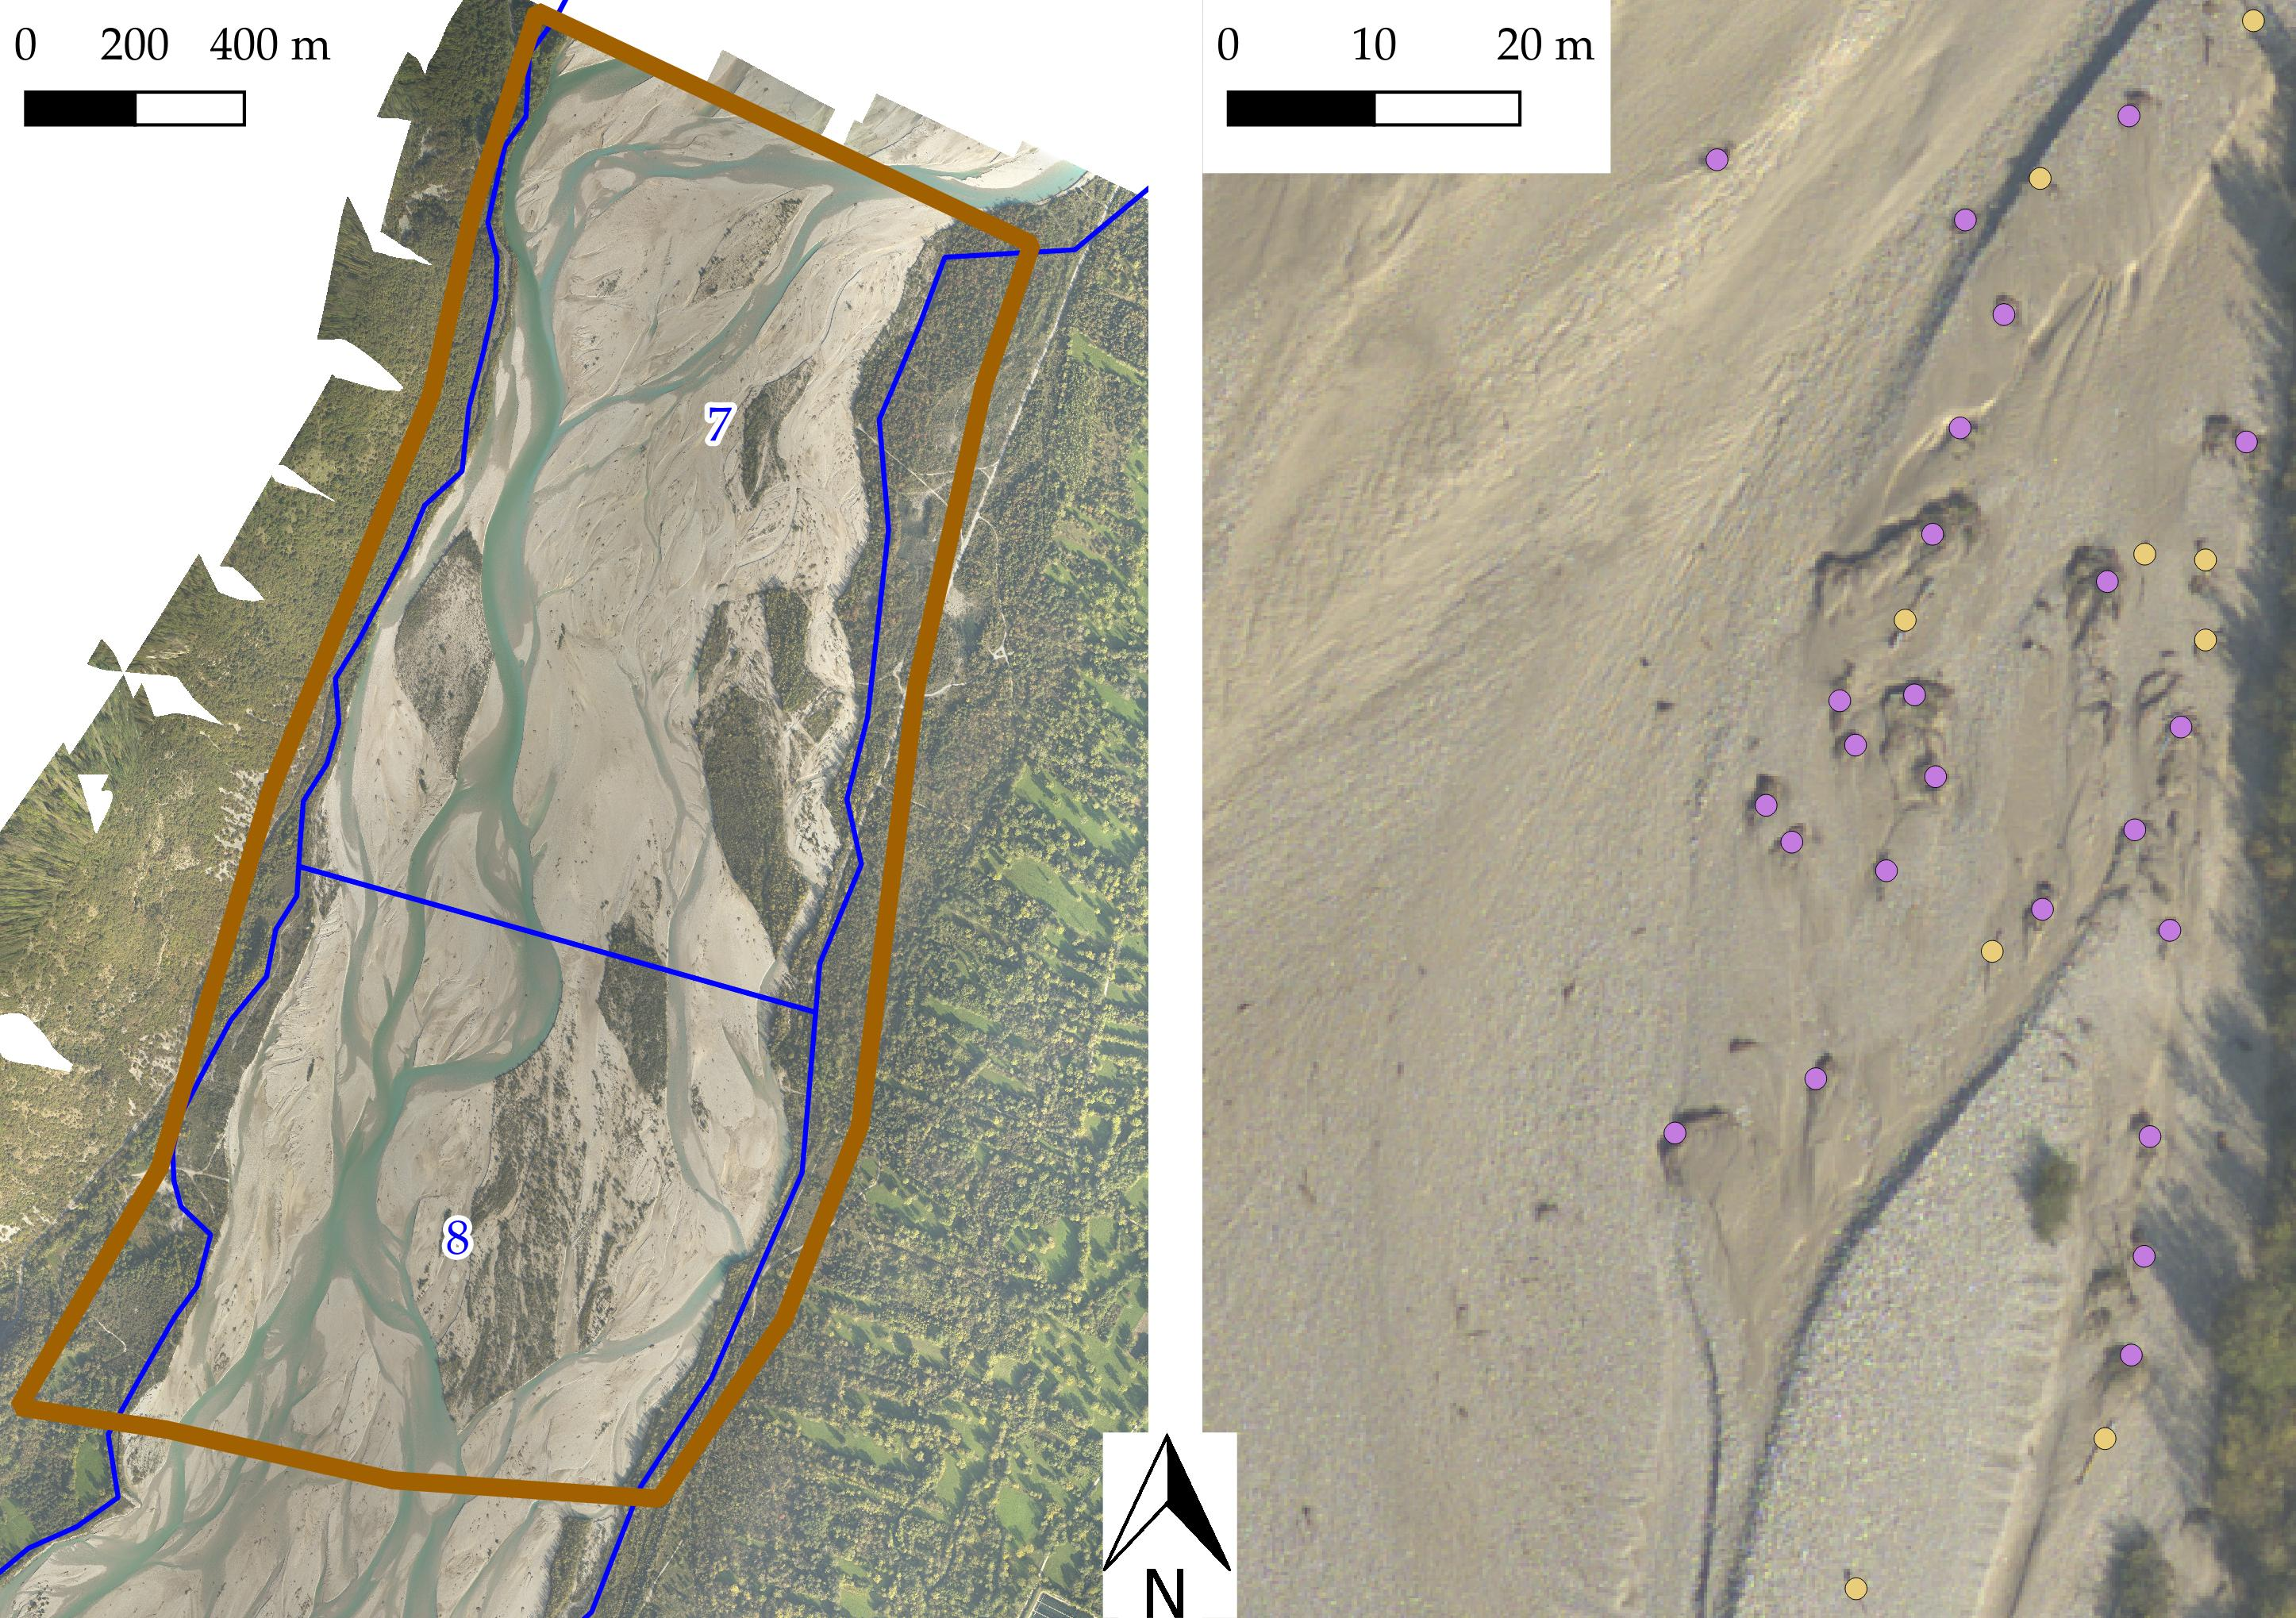
\includegraphics[width = \textwidth]{files/digitalizzazione_legno.jpeg}
	\caption[area di digitalizzazione degli elementi legnosi]{a sinistra l'area di digitalizzazione degli elementi legnosi (in marrone) e la maschera computazionale divisa in tratti (in blu); a destra un esempio di digitalizzazione in cui sono stati distinti i tronchi (in arancione) dagli accumuli (in viola); sullo sfondo è presente l'ortofoto del~2013-10-22.}
	\label{fig:digitalizzazione-legno}
\end{figure}
%
\\
In seguito per ogni digitalizzazione si è calcolata la distanza tra ogni punto e quello più vicino nella digitalizzazione successiva. Ad esempio, per ogni elemento legnoso nella mappa del~2014-10-31 è stato ottenuta la distanza dall'elemento legnoso più prossimo nella mappa del~2015-08-13.
\\
Infine per le ortofoto associate ad un rilievo LiDAR (il~2010-08 e il~2013-10-22) si è ottenuta la quota di ogni punto rispetto al DEM privo dell'effetto della pendenza (questo viene calcolato sottraendo al DEM la quota media in quella zona, cioè eliminando l'effetto della pendenza; in questo modo le quote sono riferite ad uno zero locale e mostrano chiaramente zone incise, come i canali, e zone elevate, come le barre).

\section{Risultati: erosione e accrescimento delle isole}
\label{sec:camb-ris}
I grafici in \cref{graph:erosione-matrix} e in \cref{graph:accrescimento-matrix} mostrano i rapporti tra l'erosione e l'accrescimento delle isole in ogni confronto rispetto all'area delle isole presenti inizialmente.
La data finale della mappa che si confronta corrisponde a quella delle celle colorate; la data iniziale corrisponde a quella della prima mappa valida immediatamente precedente alla data finale (cioè alla data della prima cella colorata a sinistra di ogni cella).
Con riferimento alla \cref{tab:confronti}, la mappa valida più vecchia è il~2000-09-17 per i tratti 1-21 e~2001-06-07 per i tratti~22 e~23; questa non è colorata poiché non costituisce la data finale di alcun confronto.
Il tratto~9 non viene mostrato poiché l'isola di Cornino altera i risultati, in quanto non può essere erosa.
%
\begin{figure}
	\centering
	\tikzsetnextfilename{erosione_matrix}
\begin{tikzpicture}
	\begin{axis}[
		width = 0.98\textwidth,
		height = \textwidth,
		symbolic x coords = {2000-09-17, 2001-06-07, 2002-05-18, 2002-06-12, 2003-06-22, 2004-10-14, 2005-08-30, 2006-07-16, 2007-09-21, 2008-07-05, 2009-07-08, 2010-09-29, 2011-10-02, 2012-08-01, 2013-09-05, 2014-09-08, 2014-10-31, 2015-08-13, 2015-09-12, 2015-10-22, 2016-09-13, 2017-04-21, 2017-06-13, 2018-06-15, 2018-09-16},
		xticklabel style = {
			rotate = 90,
		},
		xtick distance = 1,
		ymin = 1,
		ymax = 23,
		ytick = data,
		ylabel = {Tratto},
		y dir = reverse,
		enlargelimits = 0.02,
		colorbar horizontal,
		colorbar style = {
			xlabel = {Erosione rispetto alle isole inizialmente presenti},
			x tick label style = {
				/pgf/number format/.cd,
				fixed,
				fixed zerofill,
				precision = 1,
				/tikz/.cd,
			},
			},
		]
		\addplot[
			matrix plot*,
			mesh/cols = 23,	% per fargli leggere colonne formate da 23 righe dal file di testo
			shader = flat corner,	% per interpolare i colori
			point meta max = 1,
		]
        	table [y = tratto, x = data, point meta = \thisrow{cambiamento}] {graphics/data/erosione_matrix.txt};
    \end{axis}
\end{tikzpicture}
	\caption[erosione in tutti i confronti rispetto all'area delle isole presenti inizialmente]{erosione in tutti i confronti rispetto all'area delle isole presenti nella data iniziale del confronto; i valori sono compresi tra \numrange[range-phrase = { e }]{0}{1}, che corrispondono rispettivamente a nessuna erosione e alla completa erosione di tutte le isole.
	Ogni confronto termina in una cella colorata e comincia nella cella colorata immediatamente precedente; le mappe inizialmente valide sono il~2000-09-17 per i tratti 1-21 e~2001-06-07 per i tratti~22 e~23; nel tratto~9 è presente l'isola di Cornino, che fonda su roccia, e pertanto non viene considerato.
	Le altre celle bianche indicano assenza di dati per la limitata estensione delle immagini o per la presenza di nuvole.}
	\label{graph:erosione-matrix}
\end{figure}
%

Osservando le colonne nell'erosione, si nota che il periodo fine~2004/metà~2008 presenta generalmente bassi tassi di erosione, così come il confronto 2012-08-01/2013-09-05;
al contrario, i confronti 2008-07-05/2009-07-08 e 2012-08-11/2013-09-05 mostrano una forte erosione in quasi tutti i tratti.
Nei primi confronti non è possibile evidenziare trend spaziali data la parziale estensione delle immagini sul tratto di studio e la presenza di nuvole in pochi tratti.
\\
Considerando le righe, i tratti~12 e~23 hanno tassi elevati di erosione in quasi ogni confronto; anche i tratti più a monte subiscono molta erosione nelle isole, anche se ciò non avviene sempre.
I tratti con la larghezza maggiore, cioè i tratti 6-11 e 14-21, mostrano periodi con un'erosione relativamente più intensa alternati da periodi con erosione minore; tuttavia, aldilà dei periodi con bassi tassi di erosione evidenziati prima, non hanno un trend comune.
%
\begin{figure}
	\centering
	\tikzsetnextfilename{accrescimento_matrix}
\begin{tikzpicture}
	\begin{axis}[
		width = 0.98\textwidth,
		height = \textwidth,
		symbolic x coords = {2000-09-17, 2001-06-07, 2002-05-18, 2002-06-12, 2003-06-22, 2004-10-14, 2005-08-30, 2006-07-16, 2007-09-21, 2008-07-05, 2009-07-08, 2010-09-29, 2011-10-02, 2012-08-01, 2013-09-05, 2014-09-08, 2014-10-31, 2015-08-13, 2015-09-12, 2015-10-22, 2016-09-13, 2017-04-21, 2017-06-13, 2018-06-15, 2018-09-16},
		xticklabel style = {
			rotate = 90,
		},
		xtick distance = 1,
		ymin = 1,
		ymax = 23,
		ytick = data,
		ylabel = {Tratto},
		y dir = reverse,
		enlargelimits = 0.02,
		colorbar horizontal,
		colorbar style = {
			xlabel = {Accrescimento rispetto alle isole inizialmente presenti},
			xtick distance = 0.25,
			x tick label style = {
				/pgf/number format/.cd,
				fixed,
				fixed zerofill,
				precision = 1,
				/tikz/.cd,
			},
		},
		colormap/bluered,
		]
		\addplot[
			matrix plot*,
			mesh/cols = 23,	% per fargli leggere colonne formate da 23 righe dal file di testo
			shader = flat corner,	% per interpolare i colori
			point meta max = 3,
		]
        	table [y = tratto, x = data, point meta = \thisrow{cambiamento}] {graphics/data/accrescimento_matrix.txt};
    \end{axis}
\end{tikzpicture}
	\caption[accrescimento in tutti i confronti rispetto all'area delle isole presenti inizialmente]{accrescimento in tutti i confronti rispetto all'area delle isole presenti nella data iniziale del confronto; i valori possono essere maggiori dell'unità se le isole si sono espanse oltre l'areale iniziale.
	Ogni confronto termina in una cella colorata e comincia nella cella colorata immediatamente precedente; le mappe inizialmente valide sono il~2000-09-17 per i tratti 1-21 e~2001-06-07 per i tratti~22 e~23; nel tratto~9 è presente l'isola di Cornino, che fonda su roccia, e pertanto non viene considerato.
	Le altre celle bianche indicano assenza di dati per la limitata estensione delle immagini o per la presenza di nuvole.}
	\label{graph:accrescimento-matrix}
\end{figure}
%

Il valore massimo nel grafico dell'accrescimento è stato limitato a~\num{3} per evitare che i pochi valori molto elevati alterassero completamente la scala di colori; questi valori sono quelli del confronto 2000-09-17/2002-05-18 e quelli nel tratto~23.
\\
Ci sono stati due periodi, tra il~2004 e il~2008 e nel confronto 2011-10-02/2012-08-01, di forte crescita nella maggior parte dei tratti; anche l'ultimo confronto mostra alti tassi di crescita.
Osservando le altre righe si vede che si alternano confronti con poca crescita ad altri con una discreta espansione delle isole.
\\
Alcuni tratti, ad esempio quelli montani, il~6, il~10, il~12 o il~20, presentano generalmente accrescimenti maggiori di altri, come il~7 e il~15, dove l'espansione rispetto alle isole presenti è bassa.

I grafici in \cref{graph:eros-accr-4tr-matrix} mostrano i tassi di erosione e di accrescimento considerando gruppi di~4 tratti: l'areale del cambiamento è stata sommata sui tratti di ogni gruppo, è stata in seguito divisa per la somma delle isole presenti nei~4 tratti alla prima immagine di ogni confronto.
Il tratto~9 è stato escluso per gli stessi motivi riportati precedentemente.
%
\begin{figure}
	\centering
	\tikzsetnextfilename{eros_accr_4tr_matrix}
\begin{tikzpicture}
	\begin{axis}[
		width = \textwidth,
		height = 0.45\textwidth,
		name = erosione,
		symbolic x coords = {2000-09-17, 2001-06-07, 2002-05-18, 2002-06-12, 2003-06-22, 2004-10-14, 2005-08-30, 2006-07-16, 2007-09-21, 2008-07-05, 2009-07-08, 2010-09-29, 2011-10-02, 2012-08-01, 2013-09-05, 2014-09-08, 2014-10-31, 2015-08-13, 2015-09-12, 2015-10-22, 2016-09-13, 2017-04-21, 2017-06-13, 2018-06-15, 2018-09-16},
		xticklabel style = {
			rotate = 90,
		},
		xtick distance = 1,
		symbolic y coords = {1-4, 5-8, 10-12, 13-16, 17-20, 21-23},
		ymin = {1-4},
		ymax = {21-23},
		ytick distance = 1,
		ytick = data,
		ylabel = {Tratto},
		y dir = reverse,
		enlargelimits = 0.04,
		colorbar horizontal,
		colorbar style = {
			at = {(0.5, 1.03)},
			anchor = south,
			xticklabel pos = upper,
			xlabel = {Tasso d'erosione rispetto alle isole presenti},
%			xlabel style = {
%				rotate = 180,
%			},
		},
		]
		\addplot[
			matrix plot*,
			mesh/cols = 6,	% per fargli leggere colonne formate da 23 righe dal file di testo
			shader = flat corner,	% per interpolare i colori
			point meta max = 1,
		]
        	table [y = tratto, x = data, point meta = \thisrow{cambiamento}] {graphics/data/erosione_4tr_matrix.txt};
    \end{axis}
    
    
	\begin{axis}[
		width = \textwidth,
		height = 0.45\textwidth,
		at = {($(erosione.south) + (0cm, -2.3cm)$)},
		anchor = north,
		symbolic x coords = {2000-09-17, 2001-06-07, 2002-05-18, 2002-06-12, 2003-06-22, 2004-10-14, 2005-08-30, 2006-07-16, 2007-09-21, 2008-07-05, 2009-07-08, 2010-09-29, 2011-10-02, 2012-08-01, 2013-09-05, 2014-09-08, 2014-10-31, 2015-08-13, 2015-09-12, 2015-10-22, 2016-09-13, 2017-04-21, 2017-06-13, 2018-06-15, 2018-09-16},
		xticklabels = {,,},
		xtick distance = 1,
		symbolic y coords = {1-4, 5-8, 10-12, 13-16, 17-20, 21-23},
		ymin = {1-4},
		ymax = {21-23},
		ytick distance = 1,
		ytick = data,
		ylabel = {Tratto},
		y dir = reverse,
		enlargelimits = 0.04,
		colormap/bluered,
		colorbar horizontal,
		colorbar style = {
			at = {(0.5, -0.03)},
			anchor = north,
			xlabel = {Tasso di accrescimento rispetto alle isole presenti},
%			xlabel style = {
%				rotate = 180,
%			},
		},
		]
		\addplot[
			matrix plot*,
			mesh/cols = 6,	% per fargli leggere colonne formate da 23 righe dal file di testo
			shader = flat corner,	% per interpolare i colori
			point meta max = 3,
		]
        	table [y = tratto, x = data, point meta = \thisrow{cambiamento}] {graphics/data/accrescimento_4tr_matrix.txt};
    \end{axis}
\end{tikzpicture}
	\caption[tassi di erosione e di accrescimento unendo i tratti 4 a 4]{tassi di erosione e di accrescimento rispetto all'area delle isole presenti nella data iniziale di ogni confronto tra immagini successive; i tratti sono stati uniti in gruppi di 3 o 4.
	Ogni confronto termina in una cella colorata e comincia nella cella colorata immediatamente precedente; le mappe inizialmente valide sono il~2000-09-17 per i tratti 1-21 e~2001-06-07 per i tratti~22 e~23; il tratto~9 contiene l'isola di Cornino, che fonda su roccia, e quindi viene scartato.
	Le altre celle bianche indicano totale assenza di dati per tutti i tratti in ogni gruppo a causa della limitata estensione delle immagini o della presenza di nuvole.}
	\label{graph:eros-accr-4tr-matrix}
\end{figure}
%
\\
L'accorpamento dei tratti agisce come filtro spaziale che omogenizza le differenze più marcate che possono esserci tra tratti adiacenti; la scelta di unire i tratti di~4 in~4, come già svolto nel calcolo della pendenza, preserva le maggiori diversità spaziali che caratterizzano ogni gruppo di tratti (nel primo gruppo ci sono i tratti montani, il quarto presenta complessivamente \emph{downwelling}, e così via).
\\
È possibile osservare dei marcati trend temporali caratterizzati dall'alternanza di momenti con alti tassi d'erosione e momenti con alti tassi di crescita.
Inoltre, nei confronti dove c'è una forte erosione si vede un basso accrescimento, e viceversa.

La \cref{tab:varianza-eros-accr} mostra la varianza spaziale dei tassi di crescita ed erosione nei tratti uniti 4 a~4 (cioè calcolata su ogni colonna dei grafici in \cref{graph:eros-accr-4tr-matrix}).
La varianza è indice della dispersione dei punti: minore la varianza, più i punti hanno valori simili.
%
\begin{table}
	\centering
	\begin{tabular}{c *{2}{S[table-format = 1.3, table-comparator = true]}}
		\toprule
		{\textbf{Ultima data confronto}}	&	{\textbf{Erosione}}	&	{\textbf{Accrescimento}}	\\
		\midrule
		2001-06-17	&	0.011	&	<0.001	\\	
		2002-05-18	&	0.014	&	8.211	\\	
		2002-06-12	&	0.009	&	0.003	\\	
		2003-06-22	&	0.030	&	0.002	\\	
		2004-10-14	&	0.144	&	0.002	\\	
		2005-08-30	&	0.002	&	0.094	\\	
		2006-07-16	&	0.006	&	0.009	\\	
		2007-09-21	&	0.007	&	0.160	\\	
		2008-07-05	&	0.001	&	0.100	\\	
		2009-07-08	&	0.031	&	0.001	\\	
		2010-09-29	&	0.017	&	0.029	\\	
		2011-10-02	&	0.015	&	0.002	\\	
		2012-08-01	&	<0.001	&	0.084	\\	
		2013-09-05	&	0.018	&	<0.001	\\	
		2014-09-08	&	0.007	&	0.081	\\	
		2014-10-31	&	0.006	&	<0.001	\\	
		2015-08-13	&	0.003	&	0.011	\\	
		2015-09-12	&	0.006	&	0.005	\\
		2015-10-22	&	0.006	&	<0.001	\\
		2016-09-13	&	0.003	&	0.030	\\	
		2017-04-21	&	0.001	&	0.017	\\	
		2017-06-13	&	0.013	&	0.002	\\	
		2018-06-15	&	0.003	&	0.038	\\	
		2018-09-16	&	0.024	&	0.042	\\
		\bottomrule
	\end{tabular}
	\caption[varianza spaziale dei tassi d'erosione e accrescimento]{varianza spaziale dei tassi di erosione e accrescimento per ogni confronto tra immagini successive calcolata sui dati dei tratti uniti 4 a~4; i grafici dei tassi sono mostrati in \cref{graph:eros-accr-4tr-matrix}; la data indica l'immagine finale del confronto, pertanto il 2000-09-17 non è riportato.}
	\label{tab:varianza-eros-accr}
\end{table}
%


\section{Discussione: eventi eccezionali}
I dati relativi ai tratti più stretti, come quelli montani, il~12 (stretta di Pinzano) e il~23 (cambio morfologico), mostrano spesso alti tassi di erosione e accrescimento poiché l'areale delle isole presenti è generalmente basso (poche celle nelle immagini satellitari) e anche piccoli cambiamenti possono portare ad alte percentuali.
La soluzione di unire gruppi di~4 tratti filtra efficacemente questi casi.
\\
Dalla comparazione dei grafici di erosione e accrescimento delle isole si può vedere che quando si assiste a molta erosione, la crescita è bassa, e viceversa.
Ad esempio nel confronto 2007-09-21/2008-07-05 la crescita è alta per molti tratti e contemporaneamente l'erosione è decisamente bassa, con una varianza spaziale molto piccola (\num{0.001}); nel confronto successivo 2008-07-05/2009-07-08 si assiste ad una erosione generalizzata nel tratto di studio e, allo stesso tempo, ad un tasso di crescita ovunque bassa (varianza \num{0.001}).
La stessa situazione si ripete tra il 2011-10-02 e il 2013-09-05 e tra il 2013-09-05 e il 2014-10-31.
\\
I periodi di forte crescita sono quasi sempre seguiti da confronti che mostrano alti tassi di erosione: molto probabilmente gli anni in cui le piene sono state deboli o in cui si sono susseguite più morbide (\emph{flow pulses}) hanno incentivato la crescita delle piante e la colonizzazione di nuove aree; successivamente, gli eventi intensi di piena hanno trovato molta vegetazione in zone facilmente inondabili e l'hanno asportata.
\\
Si vede come i tratti con \emph{upwelling} più o meno pronunciato siano quelli con i maggiori tassi di crescita (come i tratti 7-11 e i tratti 17-22), mentre quelli dove la falda è in gran parte sprofondata nel materasso alluvionale, come i tratti~15 e~16, mostrano accrescimenti minori rispetto agli altri;
i tratti~4, 5 e~6, in \emph{downwelling}, è probabile che si comportino come i tratti~12 e~23: possono supportare poche isole (grafico in \cref{graph:rapp-isl-tutti-tratti}) e quando queste si espandono si moltiplicano considerevolmente, sebbene il loro areale sia particolarmente inferiore a quello di altri tratti e la loro proporzione rispetto all'alveo attivo sia bassa.
Gli effetti dell'innalzamento e dello sprofondamento della falda sono abbastanza evidenti, anche se non particolarmente marcati, nei grafici in cui si sono accorpati i tratti in gruppi da~4.
\\
Sembra che il sistema riesca efficacemente a riprendersi dopo ogni periodo di erosione intensa: nell'arco di una stagione vegetativa è possibile osservare una espansione delle isole non trascurabile.
Non ci sono tratti che si riprendono in maniera spiccatamente maggiore di altri; la ricrescita ha luogo in maniera generalizzata in tutto il fiume, come l'erosione dovuta alle piene importanti, anche se, tratto a tratto, altri fattori ambientali inducono crescite spazialmente differenziate; ciò è evidente anche dalla varianza maggiore dell'accrescimento rispetto all'erosione.
\\
Probabilmente esiste un limite dinamico di proporzione di isole che possono colonizzare l'alveo dipendente dal regime delle piene: si suppone che non esiste un'unica percentuale massima ammissibile di isole, ma che questa possa variare spazialmente e temporalmente in base agli eventi di piena e alle altre condizioni ambientali che regolano l'erosione e, più ampiamente, la crescita.

Da queste considerazioni, osservando l'idrogramma in \cref{graph:livelli-matrix} e in \cref{graph:livelli-orto-sat} (riportato a \cpageref{graph:tr-17-camb}) si può ipotizzare che le piene maggiori, come quelle avvenute verso la fine degli anni~2012 e~2014, siano quelle che abbiano asportato il maggior quantitativo di isole.
\\
I grafici in \cref{graph:tr-17-camb} mostrano alcuni risultati ottenuti dalle mappe di cambiamento per il tratto~17, posto nel tratto vallivo immediatamente a valle della confluenza con il torrente Cosa.
I dati sono rappresentati con due simboli: il pallino rappresenta la data finale di ogni confronto, mentre la croce indica la data iniziale; il pallino di un confronto ha la stessa data della croce del confronto successivo. 
La croce definisce quando inizia ogni confronto; il pallino è il dato vero e proprio.
%
\begin{figure}
	\centering
	\begin{tikzpicture}
	%\begin{groupplot}
	\begin{axis}[
		%name = orto-sat,
		axis y line* = right,
		axis x line* = top,
		%height = .3\textwidth,
		width = \textwidth,
		date coordinates in = x,
		%symbolic y coords = {ASTER,PLEIADES,SENTINEL2,G-EARTH},
		xticklabel = {\year-\month-\day},
		xtick = data,
		ytick = data,
		xticklabel style = {
			rotate = 90,
			anchor = near xticklabel
		},
		enlarge x limits = 0.05,
		enlarge y limits = 0.01,
		ylabel = {Fonte},
		ymax = 3.6,
		ymin = -0.1,
		grid = none,
		only marks,
		]
		\addplot table [x=data, y=numero] {graphics/data/data-orto-sat.txt};
	\end{axis}
	%
	\begin{axis}[
		%name = stages,
		%at = {($(orto-sat.south)-(0,2cm)$)},
		%anchor = north,
		axis y line* = left,
		width = \textwidth,
		date coordinates in = x,
		xticklabel = {\year-\month-\day},
		xticklabel style = {
			rotate = 45,
			anchor = near xticklabel
		},
		enlarge x limits = 0.05,
		enlarge y limits = 0.01,
		ymax = 3.6,
		ymin = -0.1,
		ylabel = {Livello idrometrico},
		grid = major,
		no markers,
		]
		\addplot table [x=data, y=media-gg] {graphics/data/Dati_Villuzza.csv};
	\end{axis}
\end{tikzpicture}
	\\
	\begin{tikzpicture}
	\begin{groupplot}[
		group style = {
			group size = 2 by 1,
			ylabels at = edge left,
			x descriptions at = edge bottom,
			horizontal sep = 1.1cm,
			vertical sep = 0.1cm,
		},
		width = 0.5\textwidth,
		height = 0.5\textwidth,
		date coordinates in = x,
		xticklabel = {$\year$},
		xticklabel style = {
			rotate = 80,
			anchor = near xticklabel
		},
		xtick distance = 731,
		ymax = 0.75,
		ylabel = {Cambiamento/Isole iniziali \si{[\percent]}},%\si{[\m\tothe{2}]}},
		grid = major,
		]
	\nextgroupplot % tr_17_accrescimento
		\addplot+
        	[only marks, blue]
        	table [
        		x=data_fine, 
        		y expr=\thisrow{alv->is}/808650.0
        		] {graphics/data/tr_17_camb_eros_accr.txt};
		\addplot+
        	[only marks, mark=x, black]
        	table [
        		x=data_ini, 
        		y expr=\thisrow{alv->is}/808650.0
        		] {graphics/data/tr_17_camb_eros_accr.txt};
        \node [fill = white, draw = black, anchor = south west] 
        	at (axis description cs: 0.05,0.8) {Accr.};
	\nextgroupplot % tr_17_erosione
		\addplot+
        	[only marks, blue]
        	table [
        		x=data_fine, 
        		y expr=\thisrow{is->alv}/808650.0,
        		] {graphics/data/tr_17_camb_eros_accr.txt};
		\addplot+
        	[only marks, mark=x, black]
        	table [
        		x=data_ini, 
        		y expr=\thisrow{is->alv}/808650.0,
        		] {graphics/data/tr_17_camb_eros_accr.txt};
        \node [fill = white, draw = black, anchor = south west] 
        	at (axis description cs: 0.05,0.8) {Eros.};
	\end{groupplot}
\end{tikzpicture}

	\caption[cambiamenti rilevati nelle isole nel tratto~17]{accrescimento ed erosione rilevati nelle isole del tratto~17 con le mappe dei confronti fra immagini consecutive rappresentati come percentuale rispetto all'areale delle isole nella prima data del confronto.
	Le croci indicano la data della prima immagine del confronto; i pallini indicano la data della seconda immagine del confronto, in cui si rileva il cambiamento.
	Si notano i dati relativi al periodo 2005/2008, al 2011/2012 e al 2017/2018, che mostrano valori particolarmente elevati di crescita; tranne l'ultimo confronto, di cui non si hanno dati successivi, questi sono sempre seguiti da momenti in cui la nuova vegetazione è stata erosa.}
	\label{graph:tr-17-camb}
\end{figure}
%
\\
C'è una spiccata crescita a cavallo degli anni~2005 e~2008, seguita da un'importante erosione nel~2009 (\SI{60}{\percent} delle isole presenti nel 2008).
Al contrario, nonostante la maggior intensità e durata, le piene del 2012 e del~2014 hanno eroso una percentuale inferiore di isole, forse perché ne era presente una minore quantità dato l'intervallo di una sola stagione di crescita tra piene intense.
\\
Si può supporre che la piena avvenuta alla fine del~2018 abbia rimosso gran parte delle isole che si sono formate dal~2017.
Questa osservazione può trovare la seguente giustificazione: il periodo privo di piene con livello al di sopra dei \SI{2}{\m} tra fine del~2004 e la fine del~2008 è stato favorevole per l'insediamento di nuova vegetazione, anche grazie agli eventi di morbida (\emph{flow pulses}) che hanno favorito la crescita delle piante;
le macchie vegetate sono diventate visibili da satellite solamente quando le piante hanno sviluppato una chioma sufficientemente ampia, cioè dopo qualche anno, come si nota nell'immagine del 2008-07-05;
questa più recente vegetazione si è espansa sulle barre e sulle forme morfologiche a quota minore rispetto alle isole più vecchie;
verosimilmente, la prima piena che è giunta ha facilmente portato via tutte queste isole giovani e basse.
\\
Occorre quindi ragionare non solo in termini di singoli eventi di piena, ma estendere le proprie considerazioni all'intero idrogramma, al periodo di tempo tra piene superiori ad un certo livello, alla loro frequenza, poiché sono questi i fattori che possono determinare le dinamiche delle isole.
Il periodo 2005-2008 privo di grandi piene può essere considerato un evento tanto importante quanto la piena lunga ed intensa del mese di novembre 2012.
\\
Sono presenti altri fattori, oltre al periodo privo di piene intense, che regolano la crescita: il 2001/2002 è stato un periodo con piene di piccola entità, ma non si è osservata una forte crescita; invece, il periodo 2017/2018, a cavallo di due eventi \emph{bankfull}, ha supportato quasi un raddoppio delle isole presenti.


\section{Risultati e discussione: effetti degli elementi legnosi}
È stato osservato che il legno che non viene mobilitato dalle piene è quello posto a quote relative maggiori, ad esempio su zone di deposito o sulle isole \squarecite{Gurnell:2001-island-formation}.
\\
Ogni elemento è stato individuato tramite un pallino sulla mappa; se l'elemento è esteso su più celle delle immagini, come succede nella stragrande maggioranza dei casi per i tronchi lunghi metri e gli accumuli di legno, il medesimo elemento può essere mappato in punti diversi su immagini successive.
Questo può far sembrare che il legno si sia spostato, anche se questo deriva dalla digitalizzazione manuale (ad esempio un albero depositato su una barra può essere mappato a metà del tronco o sull'apparato radicale; se viene parzialmente sepolto da un anno all'altro la mappatura può essere diversa).
Dall'altra parte, è possibile che un legno sia stato rimpiazzato da un altro: in questo caso considerare che l'elemento sia il medesimo non è corretto; tuttavia l'approccio consente di elaborare molti punti in poco tempo.
\\
È possibile per le digitalizzazioni degli elementi legnosi del~2010-08 e~2013-10-22 osservare se i tronchi e gli accumuli che si sono spostati sotto una certa soglia si trovano sulle quote relative più elevate.
La soglia può variare da \SIrange[range-phrase = { a }]{0.5}{2.5}{\m} ed è stata scelta valutando qualitativamente le digitalizzazione in anni successivi.
\\
I grafici in \cref{graph:elementi-dem-detrended-distanza} mostrano i \emph{boxplot} dei punti che hanno il legno più vicino nella digitalizzazione successiva a distanza inferiore ad una serie di soglie; l'ultimo grafico mostra invece la quota dei punti che hanno il legno più lontano della soglia nella digitalizzazione seguente.
%
\begin{figure}
	\centering
	\tikzsetnextfilename{elementi_dem_detrended_distanza}
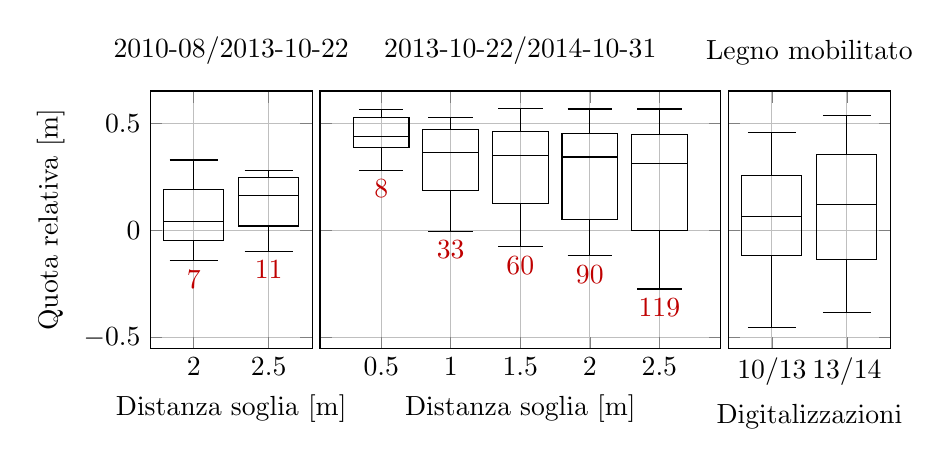
\begin{tikzpicture}
	\begin{groupplot}[
		group style = {
			group size = 3 by 1,
			y descriptions at = edge left,
			x descriptions at = edge bottom,
			horizontal sep = 0.1cm,
		},
		width = 0.38\textwidth,
		height = 0.4\textwidth,
		xlabel = {Distanza soglia \si{[\m]}},
		%xticklabel style = {font=\tiny},
		ylabel = {Quota relativa \si{[\m]}},
		boxplot/draw direction = y,
		ymax = 0.65,
		ymin = -0.55,
		%enlarge y limits = 0.05,
		grid = major,
	]
	\nextgroupplot[ % 2010/2013 elementi fermi
		width = 0.3\textwidth,
		title = {2010-08/2013-10-22},
		xtick = {1, 2},
		xticklabels = {$2$, $2.5$},
		]
		\addplot [
		        boxplot prepared = {
		                lower whisker = -0.142529,
		                lower quartile = -0.049205,
		                median = 0.042889,
		                upper quartile = 0.189542,
		                upper whisker = 0.327826,
		                },
		        ]
		        coordinates {}
				node[below, red!75!black] at (boxplot box cs: \boxplotvalue{lower whisker},0.5){\pgfmathprintnumber{7}};
		\addplot [
		        boxplot prepared = {
		                lower whisker = -0.096515,
		                lower quartile = 0.020497,
		                median = 0.163037,
		                upper quartile = 0.245633,
		                upper whisker = 0.278409,
		                },
		        ]
		        coordinates {}
				node[below, red!75!black] at (boxplot box cs: \boxplotvalue{lower whisker},0.5){\pgfmathprintnumber{11}};	
	%------------------------------------------------------
	\nextgroupplot[ % 2013/2014 elementi fermi
		width = 0.55\textwidth,
		title = {2013-10-22/2014-10-31},
		xtick = {1, 2, 3, 4, 5},
		xticklabels = {$0.5$, $1$, $1.5$, $2$, $2.5$},
		]
		\addplot [
		        boxplot prepared = {
		                lower whisker = 0.281042,
		                lower quartile = 0.385799,
		                median = 0.437347,
		                upper quartile = 0.528038,
		                upper whisker = 0.562563,
		                },
		        ]
		        coordinates {}
				node[below, red!75!black] at (boxplot box cs: \boxplotvalue{lower whisker},0.5){\pgfmathprintnumber{8}};
		\addplot [
		        boxplot prepared = {
		                lower whisker = -0.004163,
		                lower quartile = 0.187134,
		                median = 0.364044,
		                upper quartile = 0.468307,
		                upper whisker = 0.528088,
		                },
		        ]
		        coordinates {}
				node[below, red!75!black] at (boxplot box cs: \boxplotvalue{lower whisker},0.5){\pgfmathprintnumber{33}};
		\addplot [
		        boxplot prepared = {
		                lower whisker = -0.076253,
		                lower quartile = 0.124092,
		                median = 0.349297,
		                upper quartile = 0.458878,
		                upper whisker = 0.568133,
		                },
		        ]
		        coordinates {}
				node[below, red!75!black] at (boxplot box cs: \boxplotvalue{lower whisker},0.5){\pgfmathprintnumber{60}};
		\addplot [
		        boxplot prepared = {
		                lower whisker = -0.118472,
		                lower quartile = 0.050575,
		                median = 0.342194,
		                upper quartile = 0.451180,
		                upper whisker = 0.565715,
		                },
		        ]
		        coordinates {}
				node[below, red!75!black] at (boxplot box cs: \boxplotvalue{lower whisker},0.5){\pgfmathprintnumber{90}};
		\addplot [
		        boxplot prepared = {
		                lower whisker = -0.273404,
		                lower quartile = -0.001945,
		                median = 0.312073,
		                upper quartile = 0.446487,
		                upper whisker = 0.565771,
		                },
		        ]
		        coordinates {}
				node[below, red!75!black] at (boxplot box cs: \boxplotvalue{lower whisker},0.5){\pgfmathprintnumber{119}};
	%------------------------------------------------------
	\nextgroupplot[ % elementi spostati
		width = 0.3\textwidth,
		title = {Legno mobilitato},
		xlabel = {Digitalizzazioni},
		xtick = {1, 2},
		xticklabels = {10/13, 13/14},
		] % punti più distanti
		\addplot [
		        boxplot prepared = {
		                lower whisker = -0.451044,
		                lower quartile = -0.118087,
		                median = 0.065396,
		                upper quartile = 0.254933,
		                upper whisker = 0.454207,
		                },
		        ]
		        coordinates {};
		\addplot [
		        boxplot prepared = {
		                lower whisker = -0.381036,
		                lower quartile = -0.136173,
		                median = 0.120033,
		                upper quartile = 0.352123,
		                upper whisker = 0.534039,
		                },
		        ]
		        coordinates {};
	\end{groupplot}
\end{tikzpicture}

	\caption[\emph{boxplot} delle quote relative dove si trova il legno mobilitato]{\emph{boxplot} delle quote relative dove si trova il legno mobilitato nelle digitalizzazioni 2010-08/2013-10-22 (per le quali non ci sono punti con distanza minore di \SI{2}{\m}) e 2013-10-22/2014-10-31; l'ultimo grafico mostra la quota relativa del legno non mobilitato, la quale è praticamente costante per ogni soglia di distanza.
	I numeri in rosso indicano il numero di punti che definisce ogni \emph{boxplot}; per l'ultimo grafico il numero di punti è superiore a~\num{600}.}
	\label{graph:elementi-dem-detrended-distanza}
\end{figure}
%

All'aumentare della soglia ci sono più punti con distanza minima tra una digitalizzazione e la successiva minore della soglia stessa.
Per le digitalizzazioni 2010-08/2013-10-22 al di sotto della soglia di~\SI{2}{\m} i punti per ogni \emph{boxplot} sono molto pochi, da~3 a nessuno, e sono quindi stati scartati; il basso numero di punti può essere dovuto alle numerose ed intense piene che sono avvenute tra le due date, le quali hanno di sicuro mobilitato gran parte del legname presente.
Per le digitalizzazioni 2013-10-22/2014-10-31 ci sono~8 punti per la soglia più piccola di~\SI{0.5}{\m}, sufficienti per avere un \emph{boxplot} significativo.
\\
I legni che vengono mobilitati, cioè i punti che presentano distanza minima maggiore della soglia, mostrano tutti la stessa distribuzione per ogni soglia all'interno di ciascuna coppia di digitalizzazioni confrontate: praticamente a qualunque quota relativa un elemento legnoso può essere spostato oppure seppellito da depositi di ghiaia, così da non essere più visibile nella digitalizzazione successiva.
\\
Per il 2010-08/2013-10-22, i \emph{boxplot} dei punti con distanza superiore alla soglia si sovrappongono completamente a quelli con distanza inferiore alla soglia: non è possibile quindi avanzare altre ipotesi se non che, al passaggio di un gran numero di piene e di eventi importanti, il legno si sposta e che gli elementi che sembrano non essersi mobilitati in realtà sono stati rimpiazzati da altri elementi.
\\
Nelle mappe 2013-10-22/2014-10-31 al crescere della soglia di distanza massima i \emph{boxplot} si estendono verso quote minori, ma la mediana varia molto poco rimanendo circa costante ad una quota di~\SIrange[range-phrase = {-}, range-units = single]{0.3}{0.4}{\m}.
Inoltre c'è una discreta separazione tra i \emph{boxplot} delle distanze inferiori di~\SIrange[range-phrase = { e }]{0.5}{1}{\m} e il \emph{boxplot} del legno mobilitato.
Questi fatti fanno pensare che gli elementi legnosi individuati da quelle soglie siano i medesimi tra il~2013 e il~2014: le piccole piene avvenute ad inizio del~2014 possono aver spostato il legno a quote relative minori mentre il legno posto più in alto non è stato toccato.
Quest'ultimo ha la possibilità concreta di riprodursi vegetativamente ed essere il nucleo di formazione di nuove isole.
\\
I \emph{boxplot} nel grafico in \cref{graph:legno-wj-dem-detrended-distanza} mostrano la distribuzione delle quote del DEM detrended del~2013-10-22 per diverse soglie di distanza; in più, sono suddivisi gli elementi legnosi in tronchi e accumuli; infine, dalla digitalizzazione del~2013-10-22 sono considerati i tronchi che al~2014-10-31 hanno come punto più vicino un tronco, un accumulo (che potrebbe essersi formato con le piene tra le digitalizzazioni) o un elemento non riconoscibile (che potrebbe essere il tronco in parte sepolto), e gli accumuli che hanno come punto più prossimo un accumulo o un elemento non riconoscibile.
Inoltre, viene riportata la distribuzione per gli i tronchi e gli accumuli con punti nella digitalizzazione seguente dello stesso tipo e con distanza superiore alla soglia; poiché queste distribuzioni sono di fatto identiche per ogni soglia, ne viene riportata solo una.
\\
Non è riportata la soglia di~\SI{0.5}{\m} per i tronchi poiché sono presenti solo~2 punti.
Non viene riportato un grafico per il~2010-08 poiché il numero di punti risultanti da questa suddivisione non è sufficiente per avere \emph{boxplot} significativi.
%
\begin{figure}
	\centering
	\tikzsetnextfilename{legno_wj_dem_detrended_distanza}
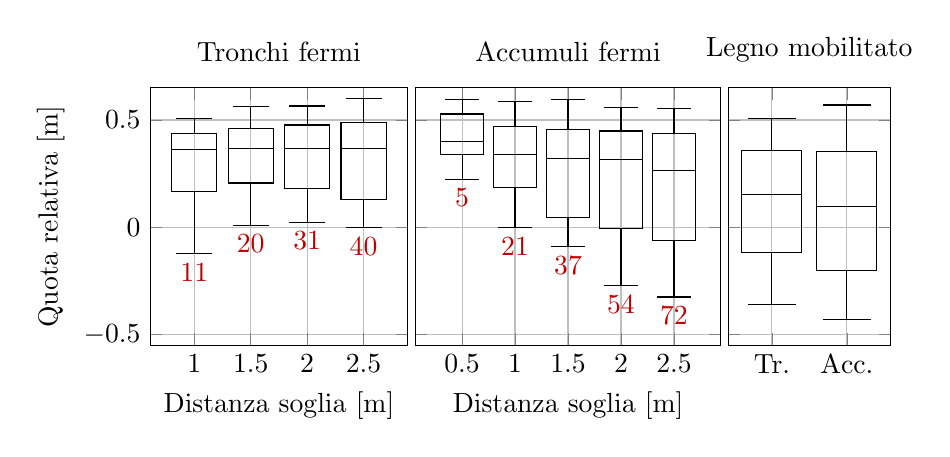
\begin{tikzpicture}
	\begin{groupplot}[
		group style = {
			group size = 3 by 1,
			y descriptions at = edge left,
			x descriptions at = edge bottom,
			horizontal sep = 0.1cm,
		},
		width = 0.38\textwidth,
		height = 0.4\textwidth,
		xlabel = {Distanza soglia \si{[\m]}},
		%xticklabel style = {font=\tiny},
		ylabel = {Quota relativa \si{[\m]}},
		boxplot/draw direction = y,
		ymax = 0.65,
		ymin = -0.55,
		%enlarge y limits = 0.05,
		grid = major,
	]
	\nextgroupplot[ % tronchi fermi
		width = 0.4\textwidth,
		title = {Tronchi fermi},
		xtick = {1, 2, 3, 4},
		xticklabels = {$1$, $1.5$, $2$, $2.5$},
		]
		\addplot [
		        boxplot prepared = {
		                lower whisker = -0.122345,
		                lower quartile = 0.167450,
		                median = 0.364044,
		                upper quartile = 0.437347,
		                upper whisker = 0.505463,
		                },
		        ]
		        coordinates {}
		node[below, red!75!black] at (boxplot box cs: \boxplotvalue{lower whisker},0.5){\pgfmathprintnumber{11}};
		\addplot [
		        boxplot prepared = {
		                lower whisker = 0.009230,
		                lower quartile = 0.206680,
		                median = 0.366295,
		                upper quartile = 0.459583,
		                upper whisker = 0.562486,
		                },
		        ]
		        coordinates {}
		node[below, red!75!black] at (boxplot box cs: \boxplotvalue{lower whisker},0.5){\pgfmathprintnumber{20}};
		\addplot [
		        boxplot prepared = {
		                lower whisker = 0.023849,
		                lower quartile = 0.180000,
		                median = 0.368546,
		                upper quartile = 0.477074,
		                upper whisker = 0.565659,
		                },
		        ]
		        coordinates {}
		node[below, red!75!black] at (boxplot box cs: \boxplotvalue{lower whisker},0.5){\pgfmathprintnumber{31}};
		\addplot [
		        boxplot prepared = {
		                lower whisker = -0.002211,
		                lower quartile = 0.127937,
		                median = 0.366295,
		                upper quartile = 0.489052,
		                upper whisker = 0.598705,
		                },
		        ]
		        coordinates {}
		node[below, red!75!black] at (boxplot box cs: \boxplotvalue{lower whisker},0.5){\pgfmathprintnumber{40}};
	%------------------------------------------------------
	\nextgroupplot[ % accumuli fermi
		width = 0.45\textwidth,
		title = {Accumuli fermi},
		xtick = {1, 2, 3, 4, 5},
		xticklabels = {$0.5$, $1$, $1.5$, $2$, $2.5$},
		]
		\addplot [
		        boxplot prepared = {
		                lower whisker = 0.223950,
		                lower quartile = 0.338135,
		                median = 0.401688,
		                upper quartile = 0.528015,
		                upper whisker = 0.596982,
		                },
		        ]
		        coordinates {}
		node[below, red!75!black] at (boxplot box cs: \boxplotvalue{lower whisker},0.5){\pgfmathprintnumber{5}};
		\addplot [
		        boxplot prepared = {
		                lower whisker = -0.002197,
		                lower quartile = 0.187134,
		                median = 0.338135,
		                upper quartile = 0.468307,
		                upper whisker = 0.585327,
		                },
		        ]
		        coordinates {}
		node[below, red!75!black] at (boxplot box cs: \boxplotvalue{lower whisker},0.5){\pgfmathprintnumber{21}};
		\addplot [
		        boxplot prepared = {
		                lower whisker = -0.090182,
		                lower quartile = 0.044922,
		                median = 0.321091,
		                upper quartile = 0.455734,
		                upper whisker = 0.595441,
		                },
		        ]
		        coordinates {}
		node[below, red!75!black] at (boxplot box cs: \boxplotvalue{lower whisker},0.5){\pgfmathprintnumber{37}};
		\addplot [
		        boxplot prepared = {
		                lower whisker = -0.273062,
		                lower quartile = -0.004040,
		                median = 0.317734,
		                upper quartile = 0.448982,
		                upper whisker = 0.557741,
		                },
		        ]
		        coordinates {}
		node[below, red!75!black] at (boxplot box cs: \boxplotvalue{lower whisker},0.5){\pgfmathprintnumber{54}};
		\addplot [
		        boxplot prepared = {
		                lower whisker = -0.325058,
		                lower quartile = -0.062695,
		                median = 0.265747,
		                upper quartile = 0.438202,
		                upper whisker = 0.554756,
		                },
		        ]
		        coordinates {}
		node[below, red!75!black] at (boxplot box cs: \boxplotvalue{lower whisker},0.5){\pgfmathprintnumber{72}};
	%------------------------------------------------------
	\nextgroupplot[ % elementi spostati
		width = 0.3\textwidth,
		title = {Legno mobilitato},
		xtick = {1, 2},
		xlabel = {},
		xticklabels = {Tr., Acc.},
		]
		\addplot [ % 500+ punti
		        boxplot prepared = {
		                lower whisker = -0.362068,
		                lower quartile = -0.118015,
		                median = 0.153465,
		                upper quartile = 0.357452,
		                upper whisker = 0.508168,
		                },
		        ]
		        coordinates {};
		\addplot [ % 300+ punti
		        boxplot prepared = {
		                lower whisker = -0.431021,
		                lower quartile = -0.199493,
		                median = 0.098511,
		                upper quartile = 0.353210,
		                upper whisker = 0.569949,
		                },
		        ]
		        coordinates {};
	\end{groupplot}
\end{tikzpicture}

	\caption[\emph{boxplot} delle quote relative distinte per tronchi e accumuli legnosi]{\emph{boxplot} delle quote relative dove si trovano tronchi (Tr.) e accumuli (Acc.) nelle digitalizzazioni 2013-10-22/2014-10-31; dopo aver calcolato la distanza dell'elemento della stessa tipologia più vicino da un'immagine all'altra, sono stati considerati gli elementi con distanza inferiore alla soglia; con la soglia~\SI{0.5}{\m} sono stati individuati solo~\num{2} tronchi, numero poco significativo e quindi scartato.
	L'ultimo grafico mostra la distribuzione dei tronchi e degli accumuli con distanza tra le digitalizzazioni superiori alle soglie; dato che queste distribuzioni sostanzialmente non variano cambiando soglia, se ne riporta solo una.
	I numeri in rosso indicano il numero di punti che definisce ogni \emph{boxplot}; per l'ultimo grafico il numero di punti è di diverse centinaia.}
	\label{graph:legno-wj-dem-detrended-distanza}
\end{figure}
%
\\
Confrontando i numeri di punti che concorrono a formare ogni \emph{boxplot}, si vede come sia maggiore il numero di accumuli che non si mobilita rispetto ai tronchi: questi ultimi differiscono dagli accumuli in quanto a conformazione, modo in cui possono essere parzialmente sepolti, resistenza offerta alla corrente (\cref{fig:tronco-vs-accumulo}).
%
\begin{figure}
	\centering
	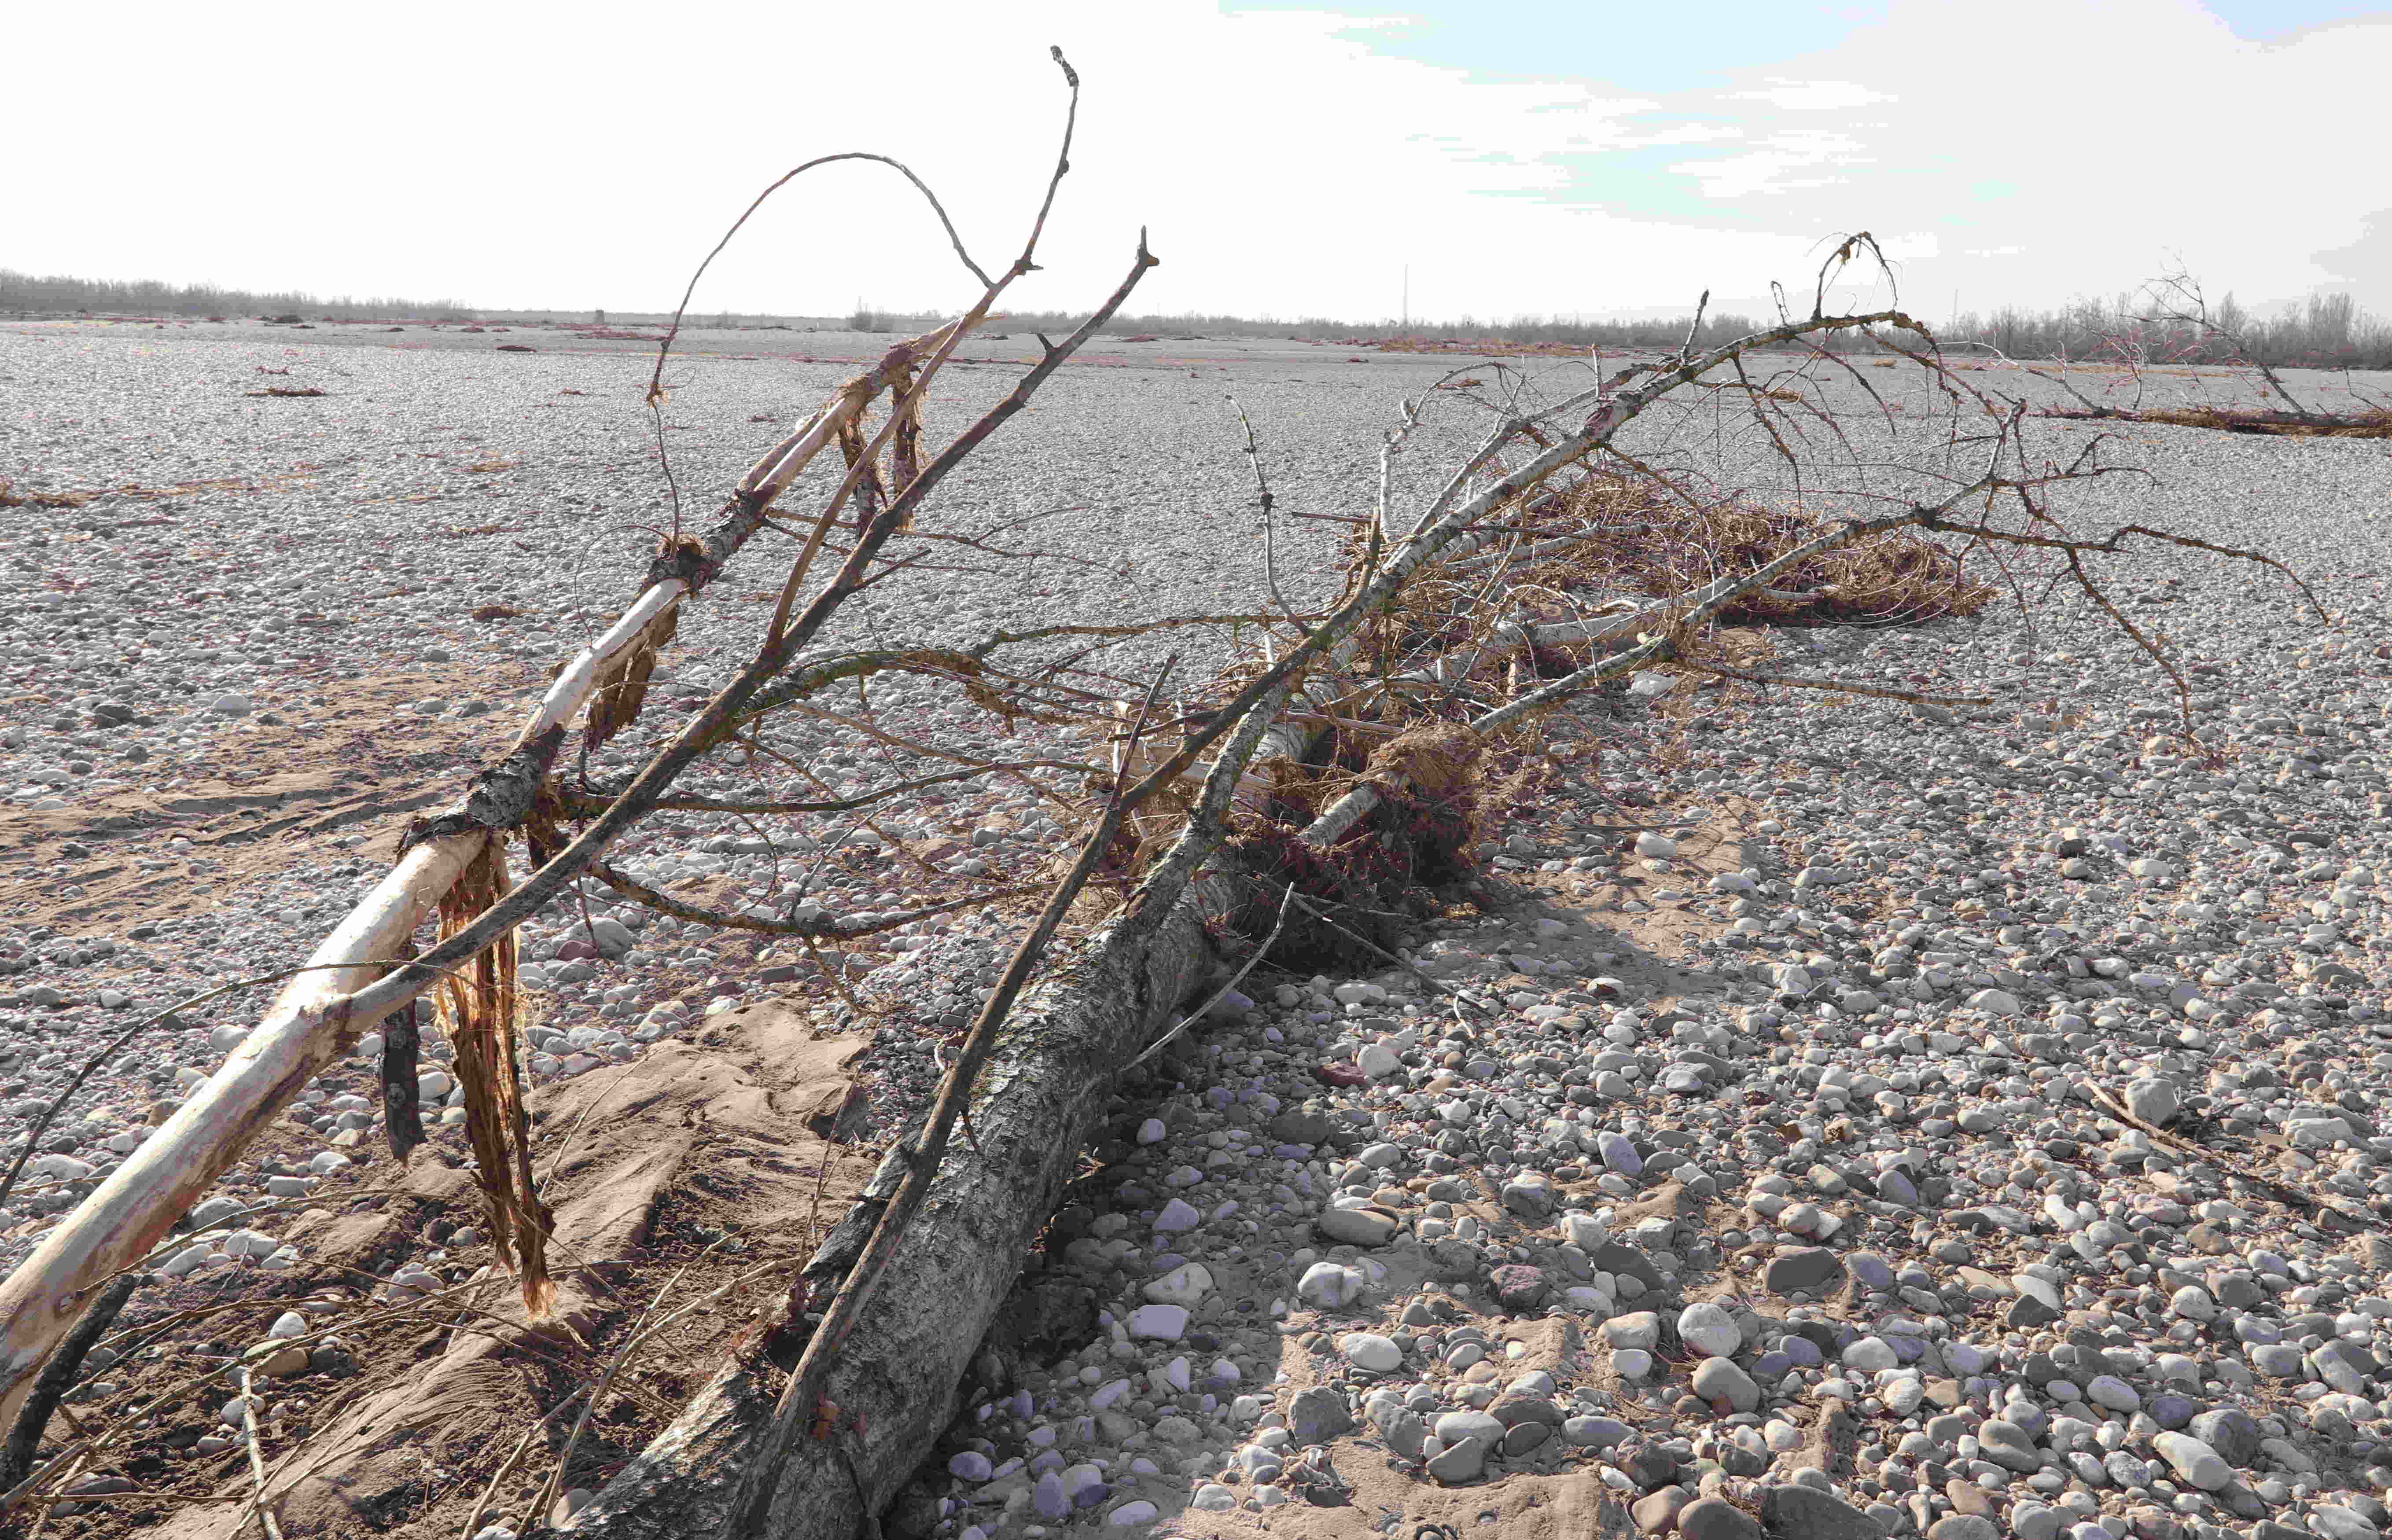
\includegraphics[height = 0.27\textwidth]{files/tronco.jpeg}
	\quad
	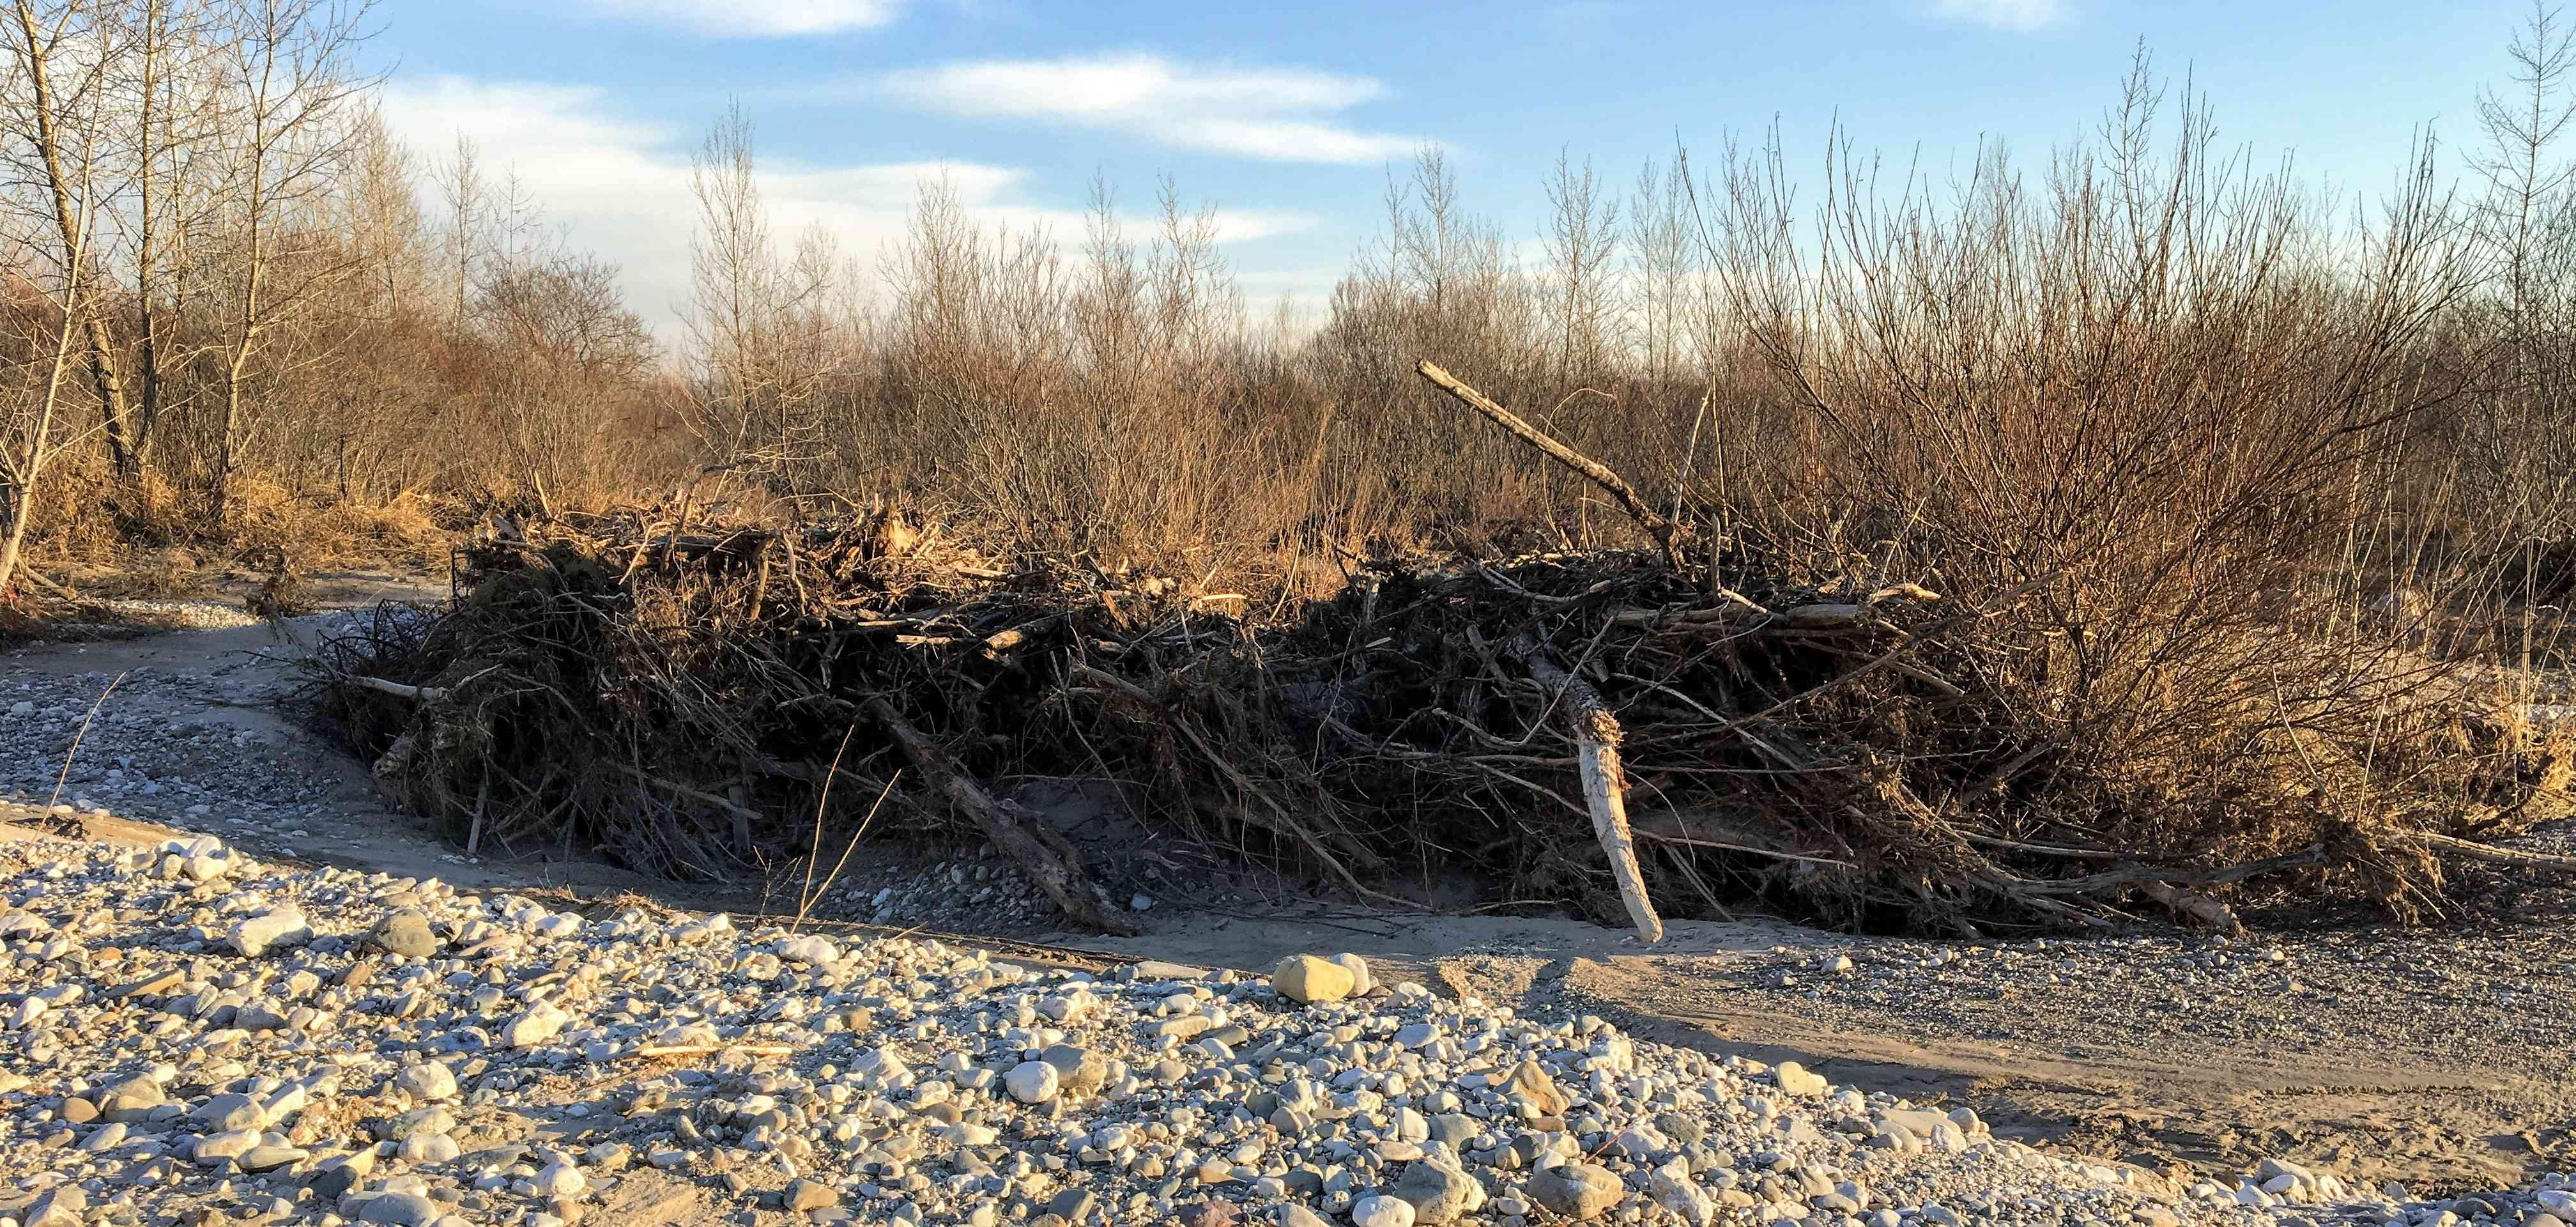
\includegraphics[height = 0.27\textwidth]{files/accumulo.jpeg}
	\caption[tronco depositato in alveo e accumulo vicino ad un'isola]{tronco depositato in alveo e accumulo vicino ad un'isola; foto scattate in data 2019-01-04 e 2019-01-05.}
	\label{fig:tronco-vs-accumulo}
\end{figure}
%
\\
La distribuzione degli accumuli, a differenza di quella dei tronchi, si allunga verso quote relative inferiori all'aumentare della distanza soglia; questo trend probabilmente è assente per i tronchi poiché questi possono resistere alle piene solo se sono stati depositati a quote elevate, mentre gli accumuli oppongono una resistenza minore.
È comprensibile quindi il motivo per cui i tronchi possono essere mobilitati più facilmente rispetto agli accumuli.
\\
Sia i tronchi che gli accumuli mantengono la mediana pressoché invariata a~\SIrange[range-phrase = {-}, range-units = single]{0.3}{0.4}{\m} per ogni soglia.
Il fatto che la mediana sia sempre superiore al terzo quartile dei \emph{boxplot} del legno mobilitato indica che gli elementi legnosi che non vengono spostati dalle piene sono quelli a quote relative più elevate, qualunque sia la tipologia di elemento.
\\
Questi risultati riflettono le numerosi osservazioni sul campo che sono state riportate da più articoli \squarecites{Gurnell:2001-island-formation}{Gurnell:2006-omega}{Bertoldi:2009-2m}{Gurnell:2014-plants-eng}.

La crescita è un fenomeno molto più lento dell'erosione ed è controllato da più fattori, come descritto nella sezione~\ref{sec:descr-area-studio}.
\\
Si è osservato tramite il confronto tra le digitalizzazioni 2014-10-31/2015-08-13 e 2015-08-13/2017 che molti degli elementi legnosi posti a quote relative elevate nel~2013-10-22 non si sono spostati fino agli anni più recenti; si è controllato se questi hanno gettato rami e foglie e se hanno formato delle isole pioniere.
Tuttavia, sembra che non ci sia stata alcuna crescita, forse a causa di una falda troppo profonda o di un substrato troppo grossolano; qualche pianta è cresciuta, ma pare che la successione biogeomorfica sia avanzata.
Dal controllo delle mappe che rilevano l'accrescimento delle isole utilizzate nelle sezioni precedenti non è stato notata alcuna nuova isola a partire da o attorno ai punti considerati.
\\
Da una parte molte piante sono cresciute a partire da semi in zone che già nell'ortofoto del~2005-05 si stavano vegetando. Il periodo 2005/2008 è stato molto favorevole per l'espansione delle isole, come già evidenziato nella sezione precedente.
Si può ipotizzare che queste isole abbiano occupato gran parte delle zone più aggradate; così non avrebbero consentito al nuovo legno di sfruttare le aree di ghiaia nuda adatte alla crescita (\cref{fig:crescita-2005-2010-2013}).
%
\begin{figure}
	\centering
	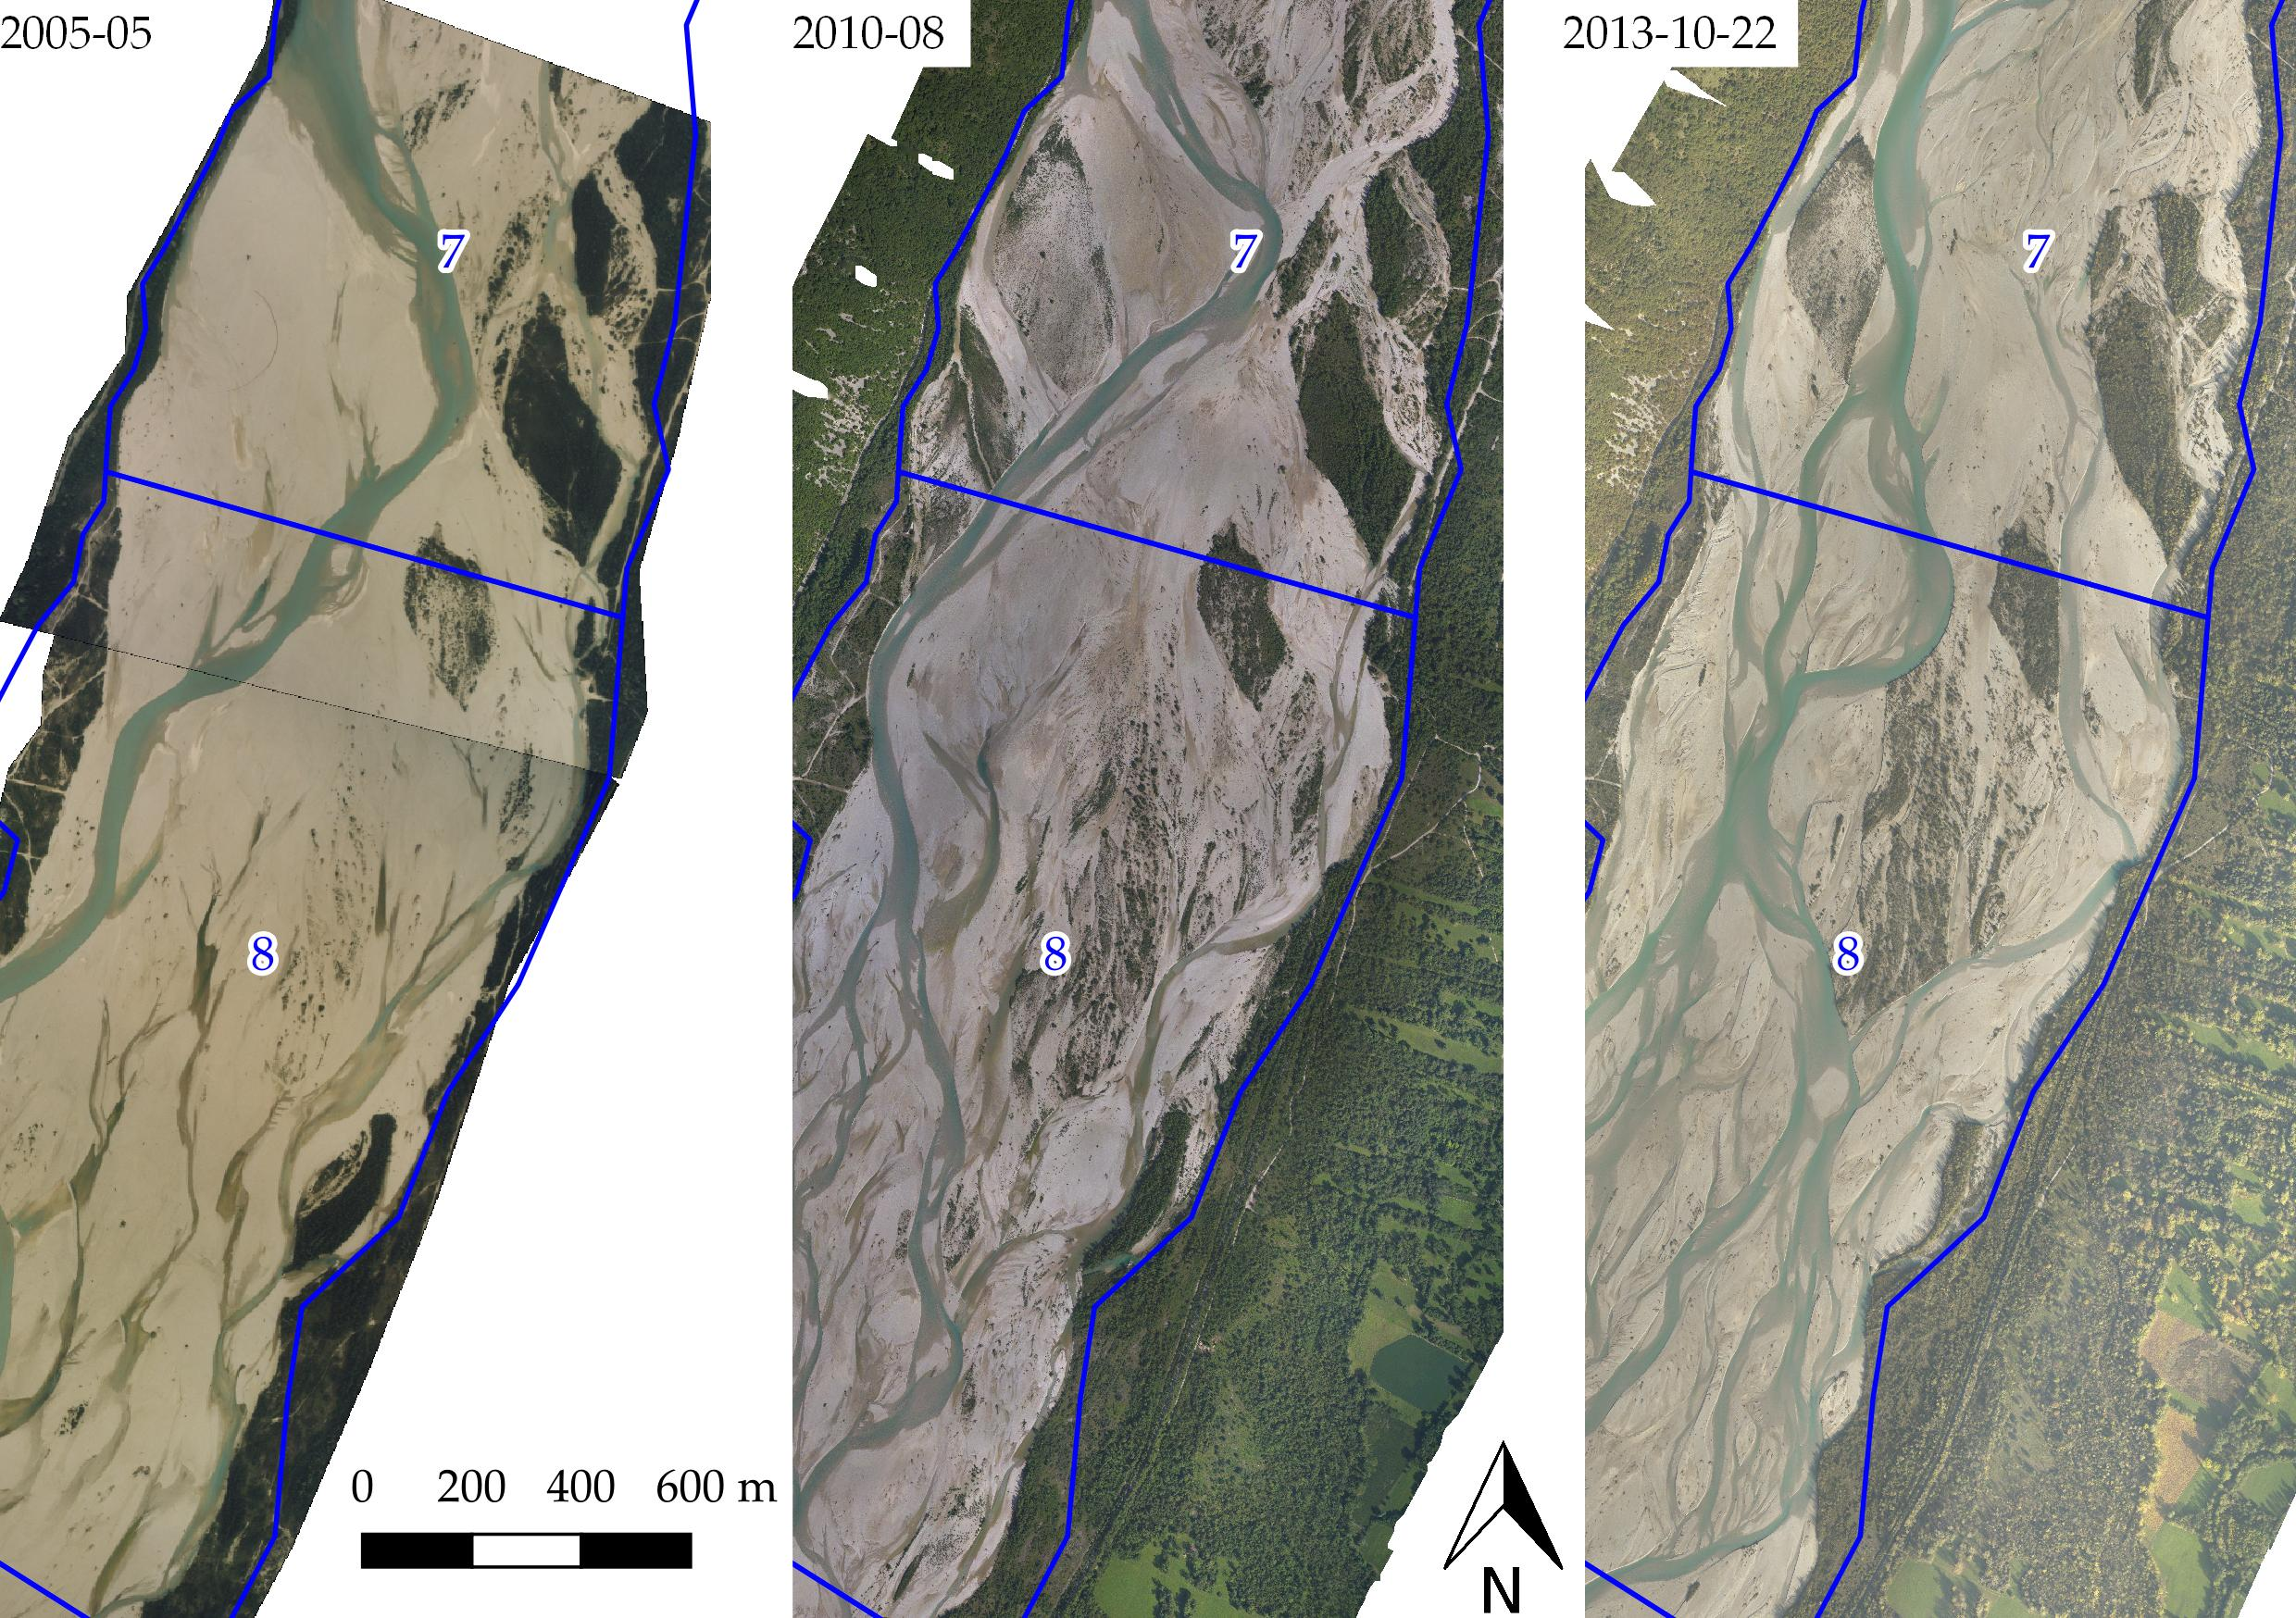
\includegraphics[width = \textwidth]{files/crescita_2005_2010_2013.jpeg}
	\caption[crescita delle isole nelle ortofoto 2005-05, 2010-08 e 2013-10-22]{crescita delle isole nelle ortofoto 2005-05, 2010-08 e 2013-10-22; si nota la forte colonizzazione di molte aree inizialmente di ghiaia nuda dal~2005-05 al~2010-08; in blu sono rappresentati i limiti della maschera computazionale divisa in tratti.}
	\label{fig:crescita-2005-2010-2013}
\end{figure}
%

%----------------------------------------------------------



\chapter{Cosa dedurre analizzando l'età delle isole?}
Utilizzando le mappe del cambiamento rilevato nelle isole si possono ottenere mappe che indicano un'età approssimativa della vegetazione che compone queste isole. 
\\
L'ipotesi che si vuole verificare è la seguente: la vegetazione più giovane, che può essere divelta più facilmente, è quella maggiormente erosa?
Si suppone di osservare erosione anche di parti di isole con vegetazione matura, poiché le aree poste in corrispondenza dell'estradosso di un canale in curva sono soggette a scavo laterale.

\section{Metodi: stimare l'età delle isole}
\label{sec:eta}

\subsection{Limiti}
Con le immagini satellitari utilizzate non è possibile distinguere i singoli alberi che compongono le isole; se con le immagini a miglior risoluzione si distinguono gli arbusti isolati, non si può certo ottenere una stima dell'età tanto precisa quanto quella fornita da un carotaggio del tronco.
In più, una cella è classificata come vegetazione solo quando le piante al suo interno presentano complessivamente una chioma sufficientemente grande da occupare gran parte della cella; pertanto le immagini con celle di \SI{10}{\m} o  \SI{15}{\m} non possono mostrare che grandi macchie di vegetazione.
Prima dei \SI{3}{\anni} una pianta di salice generalmente non ha fronde molto estese.
\\
Occorre poi tenere in conto che le piante crescono differentemente in base alle condizioni ambientali: periodi di stress idrico o termico rallentano la crescita, così come il parziale seppellimento con ghiaia dovuto ad eventi di piena; una falda non troppo profonda la cui altezza varia lentamente, terreno di granulometria sottile con sabbia e buone temperature sono invece fattori favorevoli alla crescita \squarecite{Gurnell:2001-island-formation}.

Si crede che ciò che possa generalmente accadere è che fino ad una certa età, circa \SI{3}{\anni}, la nuova vegetazione non sia visibile dal satellite; quindi si può definire come età della vegetazione presente in una cella la somma della persistenza (il periodo di tempo in cui si osserva che la cella rimane vegetata) con i \SI{3}{\anni} iniziali. 

Le mappe del cambiamento sono state ottenute dalle mappe di classificazione; non essendo le seconde correttamente georeferenziate, neanche le prime lo sono. L'errore residuo nel processo di correzione è di 1~cella.

Infine, per poter confrontare nel corso degli anni ogni cella, le mappe del cambiamento sono state ricampionate alla risoluzione più bassa, corrispondente a celle di~\SI{15}{\m} di lato. Si è proceduto come mostrato nella sottosezione \ref{subsec:camb-limiti} ottenendo sempre valori $RSQR < \SI{1.5}{\percent}$; i confronti a~\SI{10}{\m} sono stati ricampionati a~\SI{15}{\m} applicando il valore del $75_\mathrm{mo}$ percentile (terzo quartile).


\subsection{Obiettivo ed approccio} 
Date le precedenti premesse, bisogna riflettere su ciò che si vuole ottenere: dividere la vegetazione in classi di età.
Si vuole sapere quanta vegetazione giovane è stata erosa; non conta se questa ha esattamente \SI{3}{\anni} o \SI{4}{\anni}, l'importante è che sia grosso modo classificata come giovane.

Ogni mappa del cambiamento è formata dalle informazioni contenute in due mappe: quella più vecchia e quella più recente. La distanza temporale tra queste due mappe definisce il periodo di osservazione.
\\
Per la mappa del cambiamento più vecchia (la prima mappa di confronto in \cref{tab:confronti}), l'età della vegetazione delle isole è stata scelta essere pari al periodo di osservazione, cui si sono aggiunti \SI{3}{\anni}, che è ritenuto il periodo minimo affinché un insieme di piante diventi visibile per il satellite.
\\
Per le mappe via via più recenti, l'età nelle celle delle isole che non sono cambiate è pari al periodo di osservazione sommato all'età precedente; per le celle vegetate a partire dall'alveo, l'età è pari al periodo di osservazione con l'aggiunta di \SI{3}{\anni}.

L'approccio che si basa sulla definizione dell'età in base al periodo di osservazione è limitato, in particolare per le mappe più vecchie, poiché non è possibile tener conto della vegetazione che era presente antecedentemente alla prima immagine valida;
si ritiene che a partire dalla $4^a$ o $5^a$ mappa di età il metodo inizi ad essere affidabile (generalmente quindi dalla mappa di età del 2007-09-21) poiché da quel momento la vegetazione che non è stata erosa ha abbastanza anni da essere classificata come matura.
Per gli scopi della ricerca questo approccio risulta essere sufficiente.

\medskip
Si osservino i grafici in \cref{graph:distrib-rapp-eros-eta}, i quali rappresentano quante isole sono state erose rispetto alle isole presenti in ogni tratto in base all'età delle prime.
Si vede come le isole con età minore di \SI{5}{\anni} siano spesso erose; si evidenzia anche una dinamicità per le isole con età tra \SIrange[range-phrase={ e }]{5}{8}{\anni}. 
\\
Si definiscono quindi le seguenti classi di età:
%
\begin{itemize}
	\item giovane, con meno di \SI{5}{\anni};
	\item intermedia, con età compresa tra \SIrange[range-phrase={ e }]{5}{8}{\anni};
	\item matura, con più di \SI{8}{\anni}.
\end{itemize}
%
\begin{figure}
	\centering
	\tikzsetnextfilename{rapp_eros_eta}
\begin{tikzpicture}
	\begin{groupplot}[
		group style = {
			group size = 2 by 3,
			y descriptions at = edge left,
			x descriptions at = edge bottom,
			horizontal sep = 0.4cm,
			vertical sep = 0.4cm,
		},
		width = 0.54\textwidth,
		height = 0.54\textwidth,
		xlabel = {Età \si{[\anni]}},
		xmin = 3,
		xmax = 20,
		xtick distance = 3,
		enlarge x limits = 0.05,
		ylabel = {Isole erose / isole totali \si{[\percent]}},
		boxplot/draw direction = y,
		ymax = 70,
		ymin = 0,
		enlarge y limits = 0.05,
		grid = major,
	]
	\nextgroupplot % ASTER 2008_07_05
		\addplot [only marks]
			table [x=Eta, y=Perc_erosa_su_tot_isole] {graphics/data/rapp_eros_eta_2008_07_05.txt};
		\addplot [no markers, dashed, red]
			coordinates{(5,0) (5,70)};
		\addplot [no markers, dashed, red]
			coordinates{(8,0) (8,70)};
        \node [fill = white, draw = black, anchor = north east] 
        	at (axis description cs: 1,1) {AST 2008-07-05};
	%------------------------------------------------------
	\nextgroupplot % ASTER 2010_09_29
		\addplot [only marks]
			table [x=Eta, y=Perc_erosa_su_tot_isole] {graphics/data/rapp_eros_eta_2010_09_29.txt};
		\addplot [no markers, dashed, red]
			coordinates{(5,0) (5,70)};
		\addplot [no markers, dashed, red]
			coordinates{(8,0) (8,70)};
        \node [fill = white, draw = black, anchor = north east] 
        	at (axis description cs: 1,1) {AST 2010-09-29};
	%------------------------------------------------------
	\nextgroupplot % ASTER 2014_09_08
		\addplot [only marks]
			table [x=Eta, y=Perc_erosa_su_tot_isole] {graphics/data/rapp_eros_eta_2014_09_08.txt};
		\addplot [no markers, dashed, red]
			coordinates{(5,0) (5,70)};
		\addplot [no markers, dashed, red]
			coordinates{(8,0) (8,70)};
        \node [fill = white, draw = black, anchor = north east] 
        	at (axis description cs: 1,1) {AST 2014-09-08};
	%------------------------------------------------------
	\nextgroupplot % Sentinel2 2015_09_12
		\addplot [only marks]
			table [x=Eta, y=Perc_erosa_su_tot_isole] {graphics/data/rapp_eros_eta_2015_09_12.txt};
		\addplot [no markers, dashed, red]
			coordinates{(5,0) (5,70)};
		\addplot [no markers, dashed, red]
			coordinates{(8,0) (8,70)};
        \node [fill = white, draw = black, anchor = north east] 
        	at (axis description cs: 1,1) {S2 2015-09-12};
	%------------------------------------------------------
	\nextgroupplot % Sentinel2 2015_10_22
		\addplot [only marks]
			table [x=Eta, y=Perc_erosa_su_tot_isole] {graphics/data/rapp_eros_eta_2015_10_22.txt};
		\addplot [no markers, dashed, red]
			coordinates{(5,0) (5,70)};
		\addplot [no markers, dashed, red]
			coordinates{(8,0) (8,70)};
        \node [fill = white, draw = black, anchor = north east] 
        	at (axis description cs: 1,1) {S2 2015-10-22};
	%------------------------------------------------------
	\nextgroupplot % Sentinel2 2017_06_13
		\addplot [only marks]
			table [x=Eta, y=Perc_erosa_su_tot_isole] {graphics/data/rapp_eros_eta_2017_06_13.txt};
		\addplot [no markers, dashed, red]
			coordinates{(5,0) (5,70)};
		\addplot [no markers, dashed, red]
			coordinates{(8,0) (8,70)};
        \node [fill = white, draw = black, anchor = north east] 
        	at (axis description cs: 1,1) {S2 2017-06-13};
	\end{groupplot}
\end{tikzpicture}

	\caption[distribuzione del rapporto tra isole erose e la somma delle isole presenti]{distribuzione del rapporto tra le isole erose e la sommatoria di tutte le isole presenti per ogni tratto nei tratti da \numrange[range-phrase={ a }, mode=text]{1}{23} in base all'età; le linee verticali rosse tratteggiate indicano l'età di \SIrange[range-phrase={ e }]{5}{8}{\anni}.}
	\label{graph:distrib-rapp-eros-eta}
\end{figure}

\subsection{Validazione}
Da un controllo visuale delle mappe di età, si vede una corrispondenza tra struttura dell'età in diversi tipi di isole e quanto osservato da rilievi e osservazioni in campo \squarecite{Gurnell:2001-island-formation}: le isole complesse hanno una struttura d'età a macchie, mentre quelle distaccate da \emph{floodplain} hanno una struttura uniforme (\cref{fig:struttura-eta}).
%
\begin{figure}
	\centering
	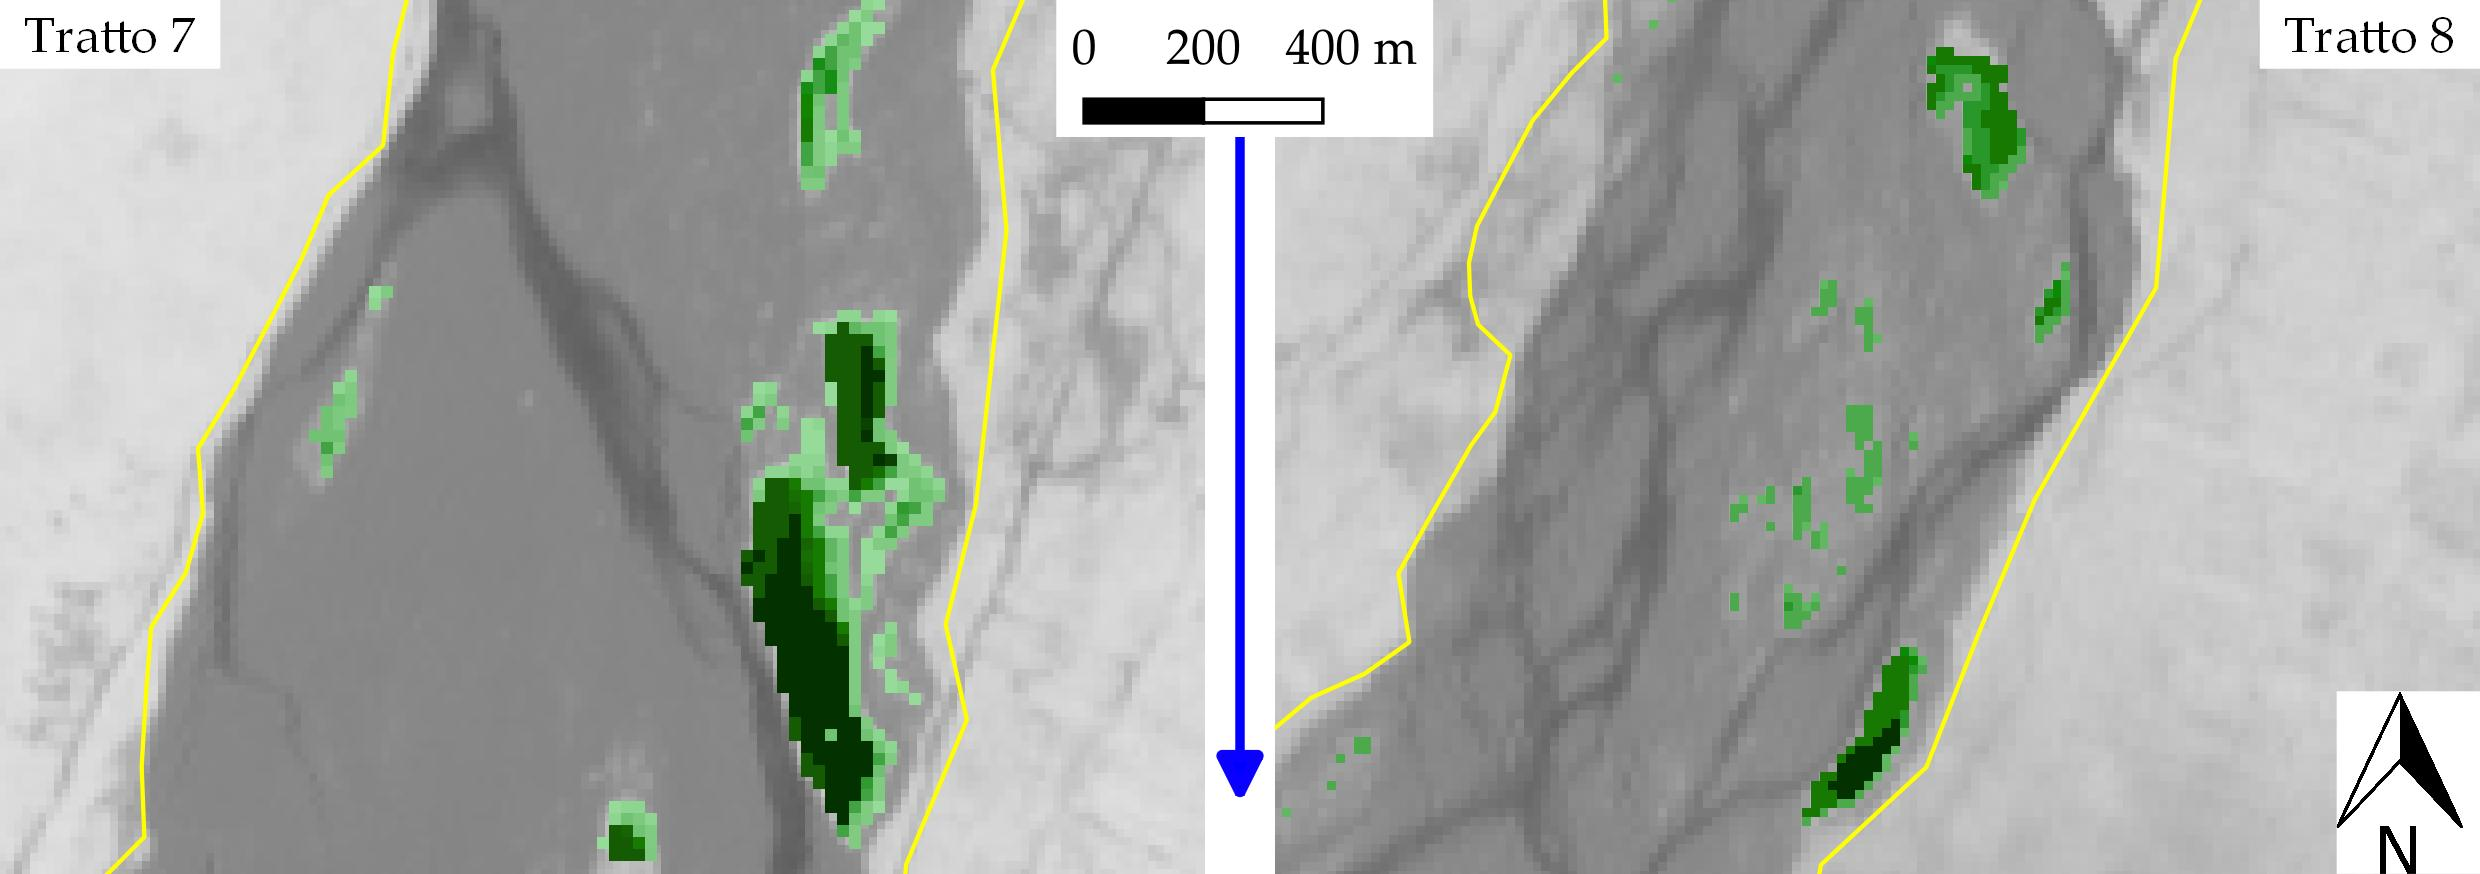
\includegraphics[width = \textwidth]{files/struttura_eta.jpeg}
	\caption[mappe della struttura di età in due tratti]{mappe della struttura di età in due tratti; i colori più scuri indicano una maggiore età.
		Nel tratto~7 (2017-06-13) si vede la struttura a macchie dell'età della vegetazione nelle isole complesse;
		nel tratto~8 (2009-07-08) si osserva la distribuzione più unifome dell'età nell'isola in basso, che si è formata dalla \emph{floodplain}.
		La maschera computazionale è mostrata in giallo; sullo sfondo sono mostrate le mappe NDVI.}
	\label{fig:struttura-eta}
\end{figure}
%

Il CHM (\emph{Canopy Height Model}) è il modello digitale della copertura arborea; similmente al DEM, mostra delle quote; queste sono tuttavia riferite all'altezza della vegetazione sopra il terreno.
\\
È generalmente sensato affermare che piante più mature abbiano un'altezza maggiore di piante giovani.
Quindi si sono utilizzati i dati di altezza della copertura arborea contenuti nei CHM di agosto~2010 e del~2013-10-22 per verificare che nelle celle della mappa di età della vegetazione, rispettivamente del~2010-09-29 e del~2013-09-05, l'altezza fosse all'incirca proporzionale all'età.
Tra le date di ottenimento dei CHM e delle immagini \AST{} non vi sono stati eventi idrologici rilevanti.
I CHM sono stati ricampionati a \SI{15}{\m} (larghezza delle celle delle immagini \AST{}) applicando il valore del $75_{\mathrm{mo}}$ percentile, in quanto rappresenta l'altezza delle chiome più elevate ed espanse, le quali dovrebbero definire i valori di età nelle mappe, essendo maggiormente visibili da satellite.
\\
Si è scelto di validare la procedura solo sulle mappe di età del~2010 e del~2013 poiché sono più rappresentative della reale distribuzione d'età delle piante, mentre la mappa di età del 2005-08-30 potrebbe non essere affidabile per quanto precedentemente esposto.
\\
I \emph{boxplot} della distribuzione dell'altezza della vegetazione rispetto all'età sono presentati nel grafico in \cref{graph:altezza-chm-eta}.
Il loro andamento crescente riflette sufficientemente quello dei dati da rilievi dendrometrici effettuati da \squarecite{Gurnell:2018-canopy-height} su isole pioniere nel Tagliamento localizzate nei medesimi tratti del CHM; pertanto ci si ritiene soddisfatti della procedura sviluppata in quanto riesce ad ottenere una stima dell'età delle piante nelle isole adeguata agli scopi della tesi.
%
\begin{figure}
	\centering
	\tikzsetnextfilename{percentili_CHM_eta}
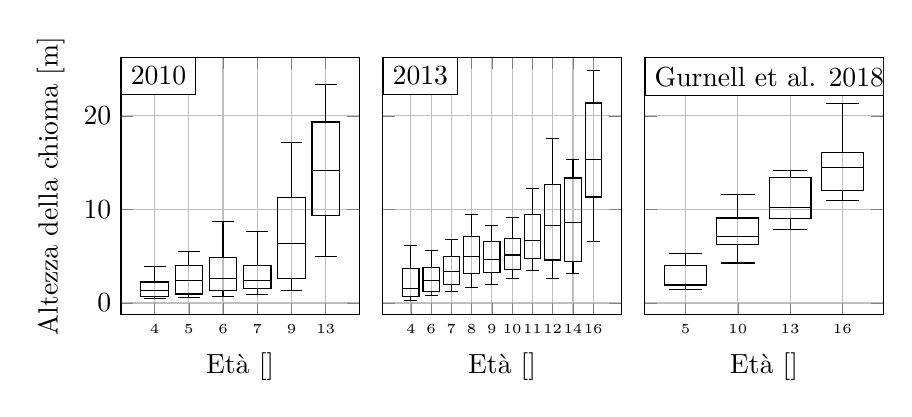
\begin{tikzpicture}
	\begin{groupplot}[
		group style = {
			group size = 3 by 1,
			y descriptions at = edge left,
			x descriptions at = edge bottom,
			horizontal sep = 0.3cm,
			vertical sep = 0.1cm,
		},
		width = 0.38\textwidth,
		height = 0.4\textwidth,
		xlabel = {Età \si{[\anni]}},
		xticklabel style = {font=\tiny},
		ylabel = {Altezza della chioma \si{[\m]}},
		boxplot/draw direction = y,
		ymax = 25,
		ymin = 0,
		enlarge y limits = 0.05,
		grid = major,
	]
	\nextgroupplot[
		xtick = {1, 2, 3, 4, 5, 6},
		xticklabels = {$4$, $5$, $6$, $7$, $9$, $13$},
		] % CSM età 2010
		\addplot [
			boxplot prepared = {
				lower whisker=0.44979499999999994,
				lower quartile=0.706821,
				median=1.349386,
				upper quartile=2.248977,
				upper whisker=3.919646,
				}
			]
			coordinates{};
		\addplot [
			boxplot prepared = {
				lower whisker=0.578308,
				lower quartile=0.963847,
				median=2.37749,
				upper quartile=4.048159,
				upper whisker=5.461802,
				}
			]
			coordinates{};
		\addplot [
			boxplot prepared = {
				lower whisker=0.706821,
				lower quartile=1.349386,
				median=2.634516,
				upper quartile=4.819237,
				upper whisker=8.700328600000006,
				}
			]
			coordinates{};
		\addplot [
			boxplot prepared = {
				lower whisker=0.9252931000000002,
				lower quartile=1.51002725,
				median=2.37749,
				upper quartile=4.0160307500000005,
				upper whisker=7.5951168,
				}
			]
			coordinates{};
		\addplot [
			boxplot prepared = {
				lower whisker=1.349386,
				lower quartile=2.634516,
				median=6.361392,
				upper quartile=11.244886,
				upper whisker=17.156482,
				}
			]
			coordinates{};
		\addplot [
			boxplot prepared = {
				lower whisker=4.94775,
				lower quartile=9.3814475,
				median=14.200684,
				upper quartile=19.341203,
				upper whisker=23.350807599999996,
				}
			]
			coordinates{};
		\node [fill = white, draw = black, anchor = north west] 
        	at (axis description cs: 0,1) {2010};
	%------------------------------------------------------
	\nextgroupplot[
		xtick = {1, 2, 3, 4, 5, 6, 7, 8, 9, 10},
		xticklabels = {$4$, $6$, $7$, $8$, $9$, $10$, $11$, $12$, $14$, $16$},
		] % CSM età 2013
		\addplot [
			boxplot prepared = {
				lower whisker=0.304544,
				lower quartile=0.657206,
				median=1.597636,
				upper quartile=3.713603,
				upper whisker=6.1352108000000065,
				}
			]
			coordinates {};
		\addplot [
			boxplot prepared = {
				lower whisker=0.774759,
				lower quartile=1.244974,
				median=2.420512,
				upper quartile=3.831157,
				upper whisker=5.594463,
				}
			]
			coordinates {};
		\addplot [
			boxplot prepared = {
				lower whisker=1.244974,
				lower quartile=1.950297,
				median=3.360942,
				upper quartile=5.006695,
				upper whisker=6.770001,
				}
			]
			coordinates {};
		\addplot [
			boxplot prepared = {
				lower whisker=1.6211462,
				lower quartile=3.125835,
				median=5.006695,
				upper quartile=7.122662,
				upper whisker=9.4972484,
				}
			]
			coordinates {};
		\addplot [
			boxplot prepared = {
				lower whisker=1.950297,
				lower quartile=3.243388,
				median=4.654033,
				upper quartile=6.534893,
				upper whisker=8.262933799999999,
				}
			]
			coordinates {};
		\addplot [
			boxplot prepared = {
				lower whisker=2.65562,
				lower quartile=3.59605,
				median=5.124248,
				upper quartile=6.9169435,
				upper whisker=9.097565300000001,
				}
			]
			coordinates {};
		\addplot [
			boxplot prepared = {
				lower whisker=3.478496,
				lower quartile=4.71281,
				median=6.652447,
				upper quartile=9.4149605,
				upper whisker=12.2009848,
				}
			]
			coordinates {};
		\addplot [
			boxplot prepared = {
				lower whisker=2.65562,
				lower quartile=4.5952565,
				median=8.2982,
				upper quartile=12.706465999999999,
				upper whisker=17.608457000000005,
				}
			]
			coordinates {};
		\addplot [
			boxplot prepared = {
				lower whisker=3.125835,
				lower quartile=4.418926,
				median=8.592084,
				upper quartile=13.35301175,
				upper whisker=15.351425,
				}
			]
			coordinates {};
		\addplot [
			boxplot prepared = {
				lower whisker=6.570159200000001,
				lower quartile=11.3252095,
				median=15.351425,
				upper quartile=21.3760555,
				upper whisker=24.8027469,
				}
			]
			coordinates {};
		\node [fill = white, draw = black, anchor = north west] 
        	at (axis description cs: 0,1) {2013};
	%------------------------------------------------------
	\nextgroupplot[
		xtick = {1, 2, 3, 4},
		xticklabels = {$5$, $10$, $13$, $16$},
		]
		\addplot [
			boxplot prepared = {
				lower whisker=1.46,
				lower quartile=1.9,
				median=1.96,
				upper quartile=3.99,
				upper whisker=5.25,
				}
			]
			coordinates {};
		\addplot [
			boxplot prepared = {
				lower whisker=4.27,
				lower quartile=6.23,
				median=7.06,
				upper quartile=9.08,
				upper whisker=11.61,
				}
			]
			coordinates {};
		\addplot [
			boxplot prepared = {
				lower whisker=7.85,
				lower quartile=8.99,
				median=10.25,
				upper quartile=13.42,
				upper whisker=14.12,
				}
			]
			coordinates {};
		\addplot [
			boxplot prepared = {
				lower whisker=10.92,
				lower quartile=12.06,
				median=14.46,
				upper quartile=16.11,
				upper whisker=21.30,
				}
			]
			coordinates {};
		\node [fill = white, draw = black, anchor = north west] 
        	at (axis description cs: 0,1) {Gurnell et al. 2018};
	\end{groupplot}
\end{tikzpicture}

	\caption[distribuzione dell'altezza delle piante secondo l'età]{distribuzione dell'altezza delle piante (dal CHM) secondo l'età (dalle mappe di età) per il 2010 e il 2013 confrontati con rilievi dendrometrici presentati da \squarecite{Gurnell:2018-canopy-height}; i grafici si riferiscono a porzioni dei tratti 6-12, dove è presente il CHM e dove sono stati effettuati i rilievi dendrometrici.}
	\label{graph:altezza-chm-eta}
\end{figure}
%



\section{Risultati: dividere l'erosione secondo l'età}
I grafici in \cref{graph:erosione-classi-eta} mostrano il rapporto tra l'areale di erosione e l'areale delle isole presenti nell'immagine iniziale dei confronti, suddiviso per le classi d'età individuate.
Non è rappresentato il tratto~9 poiché in esso è presente l'isola di Cornino; il maggior numero di dati mancanti è dovuto all'assenza di vegetazione di quella classe in alcuni tratti e in alcune immagini.
\\
La classe giovane mostra tassi di erosione maggiori di quella intermedia; questa ne presenta a sua volta di più alti rispetto alla vegetazione matura.
I confronti nei quali si era rilevata molta erosione, come il 2008-07-05/2009-07-08, il 2012-08-01/2013-09-05 e il 2014-09-08/2014-10-31, hanno subito erosione in tutte le classi d'età, anche se in maniera differenziata secondo il trend appena descritto.
\\
Non sembrano esserci tratti in cui si osserva l'erosione preferenziale di una classe d'età. Uno dopo l'altro, tutti i tratti sperimentano erosione in ogni classe, tranne per i tratti a valle di Cornino (il~10 e l'11), per i quali non si è assistito ad erosioni intense di vegetazione matura.
\\
I tratti~12 e~23 possono mostrare alte percentuali di erosione, dovute alla presenza di piccoli areali di isole, come nei grafici che mostravano il cambiamento delle isole.
%
\begin{landscape}
\begin{figure}
	\centering
	\tikzsetnextfilename{erosione_classe_eta}
\begin{tikzpicture}
	\begin{axis}[
		width = 0.49\textwidth,
		height = 0.9\textwidth,
		name = giovane,
		title = {Giovane},
		symbolic x coords = {2007-09-21, 2008-07-05, 2009-07-08, 2010-09-29, 2011-10-02, 2012-08-01, 2013-09-05, 2014-09-08, 2014-10-31, 2015-08-13, 2015-09-12, 2015-10-22, 2016-09-13, 2017-04-21, 2017-06-13, 2018-06-15, 2018-09-16},
		xticklabel style = {
			rotate = 90,
			font = \footnotesize,
		},
		xtick distance = 1,
		ymin = 1,
		ymax = 23,
		ytick = data,
		enlargelimits = 0.02,
		ylabel = {Tratto},
		y dir = reverse,
%		colorbar horizontal,
%		colorbar style = {xlabel = {Vegetazione intermedia erosa rapportata alla vegetazione intermedia presente in ogni tratto},},
		colormap/bluered,
		]
		\addplot[
			matrix plot*,
			mesh/cols = 23,	% per fargli leggere colonne formate da 23 righe dal file di testo
			shader = flat corner,	% per interpolare i colori
			point meta max = 1,
		]
        	table [y = tratto, x = data, point meta = \thisrow{cambiamento}] {graphics/data/eros_giov_matrix.txt}; 	
    \end{axis}
    
    \begin{axis}[
		width = 0.49\textwidth,
		height = 0.9\textwidth,
		name = intermedia,
		title = {Intermedia},
		at = {($(giovane.east) + (0.2cm, 0cm)$)},
		anchor = west,
		symbolic x coords = {2007-09-21, 2008-07-05, 2009-07-08, 2010-09-29, 2011-10-02, 2012-08-01, 2013-09-05, 2014-09-08, 2014-10-31, 2015-08-13, 2015-09-12, 2015-10-22, 2016-09-13, 2017-04-21, 2017-06-13, 2018-06-15, 2018-09-16},
		xticklabel style = {
			rotate = 90,
			font = \footnotesize,
		},
		xtick distance = 1,
		ymin = 1,
		ymax = 23,
		ytick = data,
		yticklabels = {,,},
		enlargelimits = 0.02,
		y dir = reverse,
%		colorbar horizontal,
%		colorbar style = {xlabel = {Vegetazione intermedia erosa rapportata alla vegetazione intermedia presente in ogni tratto},},
		colormap/bluered,
		]
		\addplot[
			matrix plot*,
			mesh/cols = 23,	% per fargli leggere colonne formate da 23 righe dal file di testo
			shader = flat corner,	% per interpolare i colori
			point meta max = 1,
		]
        	table [y = tratto, x = data, point meta = \thisrow{cambiamento}] {graphics/data/eros_int_matrix.txt};
    \end{axis}
    
    \begin{axis}[
		width = 0.49\textwidth,
		height = 0.9\textwidth,
		name = matura,
		title = {Matura},
		at = {($(intermedia.east) + (0.2cm, 0cm)$)},
		anchor = west,
		symbolic x coords = {2007-09-21, 2008-07-05, 2009-07-08, 2010-09-29, 2011-10-02, 2012-08-01, 2013-09-05, 2014-09-08, 2014-10-31, 2015-08-13, 2015-09-12, 2015-10-22, 2016-09-13, 2017-04-21, 2017-06-13, 2018-06-15, 2018-09-16},
		xticklabel style = {
			rotate = 90,
			font = \footnotesize,
		},
		xtick distance = 1,
		ymin = 1,
		ymax = 23,
		ytick = data,
		yticklabels = {,,},
		enlargelimits = 0.02,
		y dir = reverse,
		colorbar right,
		colorbar style = {
			ylabel = {Vegetazione erosa rapportata alla vegetazione presente},
			ylabel style = {
				rotate = 180,
			},
		},
		colormap/bluered,
		]
		\addplot[
			matrix plot*,
			mesh/cols = 23,	% per fargli leggere colonne formate da 23 righe dal file di testo
			shader = flat corner,	% per interpolare i colori
			point meta max = 1,
		]
        	table [y = tratto, x = data, point meta = \thisrow{cambiamento}] {graphics/data/eros_mat_matrix.txt};
    \end{axis}
\end{tikzpicture}
	\caption[erosione di ogni classe d'età rispetto alle isole presenti]{erosione di ogni classe d'età rispetto alle isole presenti; sono mostrate solamente le immagini a partire dal~2007; il tratto~9 non è stato considerato.}
	\label{graph:erosione-classi-eta}
\end{figure}
\end{landscape}
%

\section{Discussione: un trend per la vegetazione erosa}
Il periodo con assenza di piene intense tra il~2005 e il~2008 ha portato ad un forte incremento della vegetazione, che in seguito è stata erosa durante gli eventi successivi di piena.
La maggior parte della vegetazione erosa è stata quella giovane cresciuta negli anni precedenti, mentre la percentuale di erosione nelle altre classi d'età è stata molto minore, sebbene presente.
Dinamiche simili hanno avuto luogo tra il~2011 e il~2013: un periodo favorevole per la crescita ha sperimentato una forte erosione a causa delle intense piene che sono succedute.
\\
Nel periodo 2011-10-02/2012-08-01 si è rilevata una non trascurabile espansione delle isole e ci sono state poche piene rilevanti; l'erosione è stata molto debole, quasi assente in ogni classe. Forse le piene avvenute prima di questo periodo hanno asportato gran parte della vegetazione e le poche piene oltre i \SI{2}{\m} che sono arrivate tra il~2011 e il~2012 non hanno trovato piante in zone facilmente inondabili.
\\
A seguito dell'evento \emph{bankfull} della fine del~2012 e dei \emph{flood pulses} tra il~2013 e il~2014 molte isole mature sono state erose nei tratti vallivi; il loro tasso di erosione è paragonabile a quello rilevato nelle isole giovani ed intermedie. Queste piene sono riuscite ad avere un effetto di cui non se ne osservano pari; i periodi di crescita che hanno preceduto questo evento potrebbero aver favorito la crescita di isole in zone relativamente più protette dalle piene, quali le zone a quota relativa più alta, mentre molte altre piante giovani ed intermedie sono state travolte; la piena più importanta e rara di fine~2012 è riuscita ad erodere molta della vegetazione sopravvissuta ormai matura perché ne era presente una grande quantità e in aree non ancora aggradatesi particolarmente.
C'è comunque da ricordare che anche piene poco importanti possono erodere isole insediatesi in alveo da tempo, come mostrano le celle con tassi considerevoli di erosione della componente matura sparse nel grafico, poiché, se queste si trovano all'estradosso di canali in curva, possono crollare per scalzamento al piede dell'isola.
\\
Riassumendo, sembra che le possibilità di erosione in una classe dipendano sia dalla disponibilità di isole da erodere, sia dal regime delle piene che ha preceduto il momento che si sta osservando.

Si considerino le isole presenti in alcuni tratti e alcune immagini, divise per classi di età; si considerino anche le isole erose in seguito alle immagini di cui sopra, divise per classi di età e nei medesimi tratti: ciò che si vede nel grafico in \cref{graph:distr-eta} è la quantità di isole erose per ogni classe, rispetto alle isole presenti. 
%
\begin{figure}
	\centering
	\tikzsetnextfilename{eta_tratti_8_11_17}
\begin{tikzpicture}
	\begin{groupplot}[
		group style = {
			group size = 3 by 1,
			x descriptions at = edge bottom,
			y descriptions at = edge left,
			xticklabels at = all,
			horizontal sep = 0.2cm,
			vertical sep = 0.25cm,
		},
		width = 0.37\textwidth,
		height = 0.8\textwidth,
	    xbar stacked,
		enlarge x limits = 0.02,
		enlarge y limits = 0.10,
		symbolic y coords = {
			2008-07-05, 2009-07-08, 
			2012-08-01, 2013-09-05,  
			2016-09-13, 2017-06-13
		},
		ytick distance = 1,
		%scaled x ticks = false,
		xlabel = {Areale \si{[\m\tothe{2}]}},
		xmajorgrids = true,
		]
		\nextgroupplot % tratto_8
			\addplot[bar shift = .4cm, pattern = north east lines]
		       	table [y=data, x=giovane-e] {graphics/data/tr_8_eta.txt};
			\addplot[bar shift = .4cm, fill = green]
		       	table [
		       		y=data, 
		       		x expr=\thisrow{giovane} - \thisrow{giovane-e}
		       		] {graphics/data/tr_8_eta.txt};
		       		
			\resetstackedplots
			\addplot[bar shift = 0cm, pattern = north east lines, forget plot]
		       	table [y=data, x=interm-e] {graphics/data/tr_8_eta.txt};
			\addplot[bar shift = 0cm, fill = green!75!black]
		       	table [
		       		y=data, 
		       		x expr=\thisrow{interm} - \thisrow{interm-e}
		       		] {graphics/data/tr_8_eta.txt};
		       		
			\resetstackedplots
			\addplot[bar shift = -.4cm, pattern = north east lines, forget plot]
		       	table [y=data, x=matura-e] {graphics/data/tr_8_eta.txt};
			\addplot[bar shift = -.4cm, fill = green!40!black]
		       	table [
		       		y=data, 
		       		x expr=\thisrow{matura} - \thisrow{matura-e}
		       		] {graphics/data/tr_8_eta.txt};
		    
        	\node [fill = white, draw = black, anchor = north east] 
        		at (axis description cs: 1,1) {Tr. 8};
        %
		\nextgroupplot [% tratto_11
			legend style = {
				at = {(0.5,1.02)},
				legend columns = 4,
				anchor = south
			}, 
			]
			\addplot[bar shift = .4cm, pattern = north east lines]
		       	table [y=data, x=giovane-e] {graphics/data/tr_11_eta.txt};
		    \addlegendentry{Erosione}
			\addplot[bar shift = .4cm, fill = green]
		       	table [
		       		y=data, 
		       		x expr=\thisrow{giovane} - \thisrow{giovane-e}
		       		] {graphics/data/tr_11_eta.txt};
		    \addlegendentry{Giovane}
		       		
			\resetstackedplots
			\addplot[bar shift = 0cm, pattern = north east lines, forget plot]
		       	table [y=data, x=interm-e] {graphics/data/tr_11_eta.txt};
			\addplot[bar shift = 0cm, fill = green!75!black]
		       	table [
		       		y=data, 
		       		x expr=\thisrow{interm} - \thisrow{interm-e}
		       		] {graphics/data/tr_11_eta.txt};
		    \addlegendentry{Intermedia}
		       		
			\resetstackedplots
			\addplot[bar shift = -.4cm, pattern = north east lines, forget plot]
		       	table [y=data, x=matura-e] {graphics/data/tr_11_eta.txt};
			\addplot[bar shift = -.4cm, fill = green!40!black]
		       	table [
		       		y=data, 
		       		x expr=\thisrow{matura} - \thisrow{matura-e}
		       		] {graphics/data/tr_11_eta.txt};
		    \addlegendentry{Matura}
		    
        	\node [fill = white, draw = black, anchor = north east] 
        		at (axis description cs: 1,1) {Tr. 11};
        	%
        	
		\nextgroupplot % tratto_17
			\addplot[bar shift = .4cm, pattern = north east lines]
		       	table [y=data, x=giovane-e] {graphics/data/tr_17_eta.txt};
			\addplot[bar shift = .4cm, fill = green]
		       	table [
		       		y=data, 
		       		x expr=\thisrow{giovane} - \thisrow{giovane-e}
		       		] {graphics/data/tr_17_eta.txt};
		       		
			\resetstackedplots
			\addplot[bar shift = 0cm, pattern = north east lines, forget plot]
		       	table [y=data, x=interm-e] {graphics/data/tr_17_eta.txt};
			\addplot[bar shift = 0cm, fill = green!75!black]
		       	table [
		       		y=data, 
		       		x expr=\thisrow{interm} - \thisrow{interm-e}
		       		] {graphics/data/tr_17_eta.txt};
		       		
			\resetstackedplots
			\addplot[bar shift = -.4cm, pattern = north east lines, forget plot]
		       	table [y=data, x=matura-e] {graphics/data/tr_17_eta.txt};
			\addplot[bar shift = -.4cm, fill = green!40!black]
		       	table [
		       		y=data, 
		       		x expr=\thisrow{matura} - \thisrow{matura-e}
		       		] {graphics/data/tr_17_eta.txt};
		    
        	\node [fill = white, draw = black, anchor = north east] 
        		at (axis description cs: 1,1) {Tr. 17};
	\end{groupplot}
\end{tikzpicture}




	\caption[areale delle isole e dell'erosione subita divise in classi d'età per i tratti~8, 11 e~17]{areale delle isole e dell'erosione subita dalle isole stesse, entrambe divise in classi d'età, per alcune immagini per i tratti~8, 11 e~17.}
	\label{graph:distr-eta}
\end{figure}
%
Focalizzandosi sugli eventi di piena della fine del~2008 e del~2012, si vede chiaramente come l'areale della vegetazione giovane sia stato fortemente eroso (tratti \numrange[range-phrase={ e }]{11}{17});
sia in termini relativi che in termini assoluti, la vegetazione giovane è quella che è prevalentemente portata via dalle piene.
\\
Questo è molto probabilmente dovuto alla colonizzazione delle piante delle zone a quota medio-elevata, come le creste delle barre, durante il periodo tra due piene; 
se le condizioni ambientali sono adatte, se non hanno luogo piene particolarmente intense ma piene di piccola-media entità (\emph{flow pulses}) allora le piante possono crescere ottimamente e le isole si accrescono, come riportato nella sezione introduttiva~\ref{sec:descr-area-studio}.
\\
Il periodo compreso tra il~2005 e il~2008 molto probabilmente è stato caratterizzato da condizioni idrologiche ottimali per la crescita di nuova vegetazione, come già osservato nella sezione~\ref{sec:camb-ris}.
Ora è possibile affermare che la forte erosione osservata dall'immagine del cambiamento 2008-07-05/2009-07-08 si è concentrata sulla vegetazione giovane.
\\
Data la ricolonizzazione per via vegetativa di \emph{Populus nigra} e \emph{Salix spp.} che ha luogo dopo ogni piena da parte di tronchi depositati su barre e attorno a isole già esistenti, la presenza di piante giovani è quasi costante.

Momenti in cui non ci sono state piene con livello oltre i~\SI{2}{\m}, come nei periodi 2013-2014 e 2015-2017, mostrano che l'erosione delle isole è stata modesta, di entità ben minore rispetto a quanto appena esposto. Tuttavia, nella classe giovane, l'erosione presenta spesso tassi elevati anche in seguito a periodi in cui il tasso di crescita è basso, ad esempio nel~2011-10-02 (grafico in \cref{graph:accrescimento-matrix}).
A meno di eventi molto intensi o di isole poste all'estradosso di canali, la componente giovane delle isole è quella che viene asportata per prima.
%Si tenga comunque in conto che parte della vegetazione non erosa invecchia e può passare da una classe a quella successiva; questo fenomeno non è tuttavia quello predominante durante le piene del~2008 e del~2012 per evidenza.


%----------------------------------------------------------



\chapter{Quali sono le relazioni tra piene e dinamiche delle isole?}
Con i dati a disposizione è possibile ricercare delle relazioni che leghino il regime delle piene con la dinamica delle isole.
Poiché l'erosione delle isole è solamente legata agli effetti delle piene, mentre l'accrescimento è influenzato da più fattori (come è stato spiegato nella sezione~\ref{sec:descr-area-studio}), l'analisi esclude quest'ultimo.

\section{Metodi: parametri considerati}

\paragraph{Isole erose}
Dallo studio dei cambiamenti delle isole tra un'immagine e quella successiva si sono ottenuti i dati di areale di isole erose (sezione~\ref{sec:cambiamento});
questi dati sono stati suddivisi secondo tre classi di età della vegetazione: giovane, intermedia e matura (sezione~\ref{sec:eta}).
Quindi è nota la quantità di isole erose a cavallo di ogni immagine, in ogni tratto e per ogni classe di età.

\paragraph{Integrale dei livelli}
Dai dati di livello dell'acqua presso la stazione idrometrica di Villuzza, alcuni autori hanno ottenuto una statistica dei tempi di ritorno dei picchi delle piene superiori ad \SI{1}{\m} \squarecite{Bertoldi:2009-2m}; questa è stata estesa utilizzando i dati di livello idrometrico dal~2000-01-01 al~2018-12-21 ed è riportata nel grafico in \cref{graph:tr-picchi}; in totale sono stati individuati poco più di~200 picchi.
%
\begin{figure}
	\centering
	\tikzsetnextfilename{tr_picchi}
\begin{tikzpicture}
	\begin{semilogxaxis}[
		width = \textwidth,
		height = 0.5\textwidth,
%		enlarge x limits = 0.05,
%		enlarge y limits = 0.01,
%		ytick distance = 0.5,
		ylabel = {Livello idrometrico \si{[\m]}},
		xlabel = {Tempo di ritorno \si{[\anni]}},
		y tick label style = {
			/pgf/number format/.cd,
			fixed,
			fixed zerofill,
			precision = 1,
			/tikz/.cd,
		},
		grid = major,
        log ticks with fixed point,		
		]
		\addplot
        	[blue, no markers]
        	table [x=tr_anni, y=picchi] {graphics/data/tr_picchi.txt};
        
        \draw[<->] (0.1,3) -- (0.5,3);
        \node [at = {(0.23,3)}, anchor = north] {\emph{Flow pulses}};
        
        \draw[<->] (0.5,1) -- (3,1);
        \node [at = {(1.3,1)}, anchor = south] {\emph{Flood pulses}};
        
        \draw[<->] (3,1) -- (20,1);
        \node [at = {(7,1)}, anchor = south] {\emph{Bankfull}};
	\end{semilogxaxis}
\end{tikzpicture}
	\caption[tempi di ritorno dei picchi superiori ad \SI{1}{\m}]{tempi di ritorno dei picchi superiori ad \SI{1}{\m} ottenuti dall'individuazione di più di 200 picchi dai dati idrometrici.}
	\label{graph:tr-picchi}
\end{figure}
%
\\
Non sono stati utilizzati i massimi annuali poiché piene con tempo di ritorno inferiore ad \SI{1}{\anno} hanno anch'esse importi effetti sulla morfologia del fondo e sulle isole.
\\
La statistica effettuata da \squarecite{Bertoldi:2009-2m} utilizzava i dati dal~1981 al~2007.
Nel presente lavoro non sono stati utilizzati dati idrometrici anteriori al~1981 poiché precedentemente i livelli erano manualmente letti su un'asta graduata in un singolo momento della giornata; si capisce che questi dati sono molto meno affidabili di quelli rilevati con intervallo orario o semi orario, che sono in grado di descrivere dettagliatamente il passaggio di ogni piena.
Sono stati utilizzati solo i dati dal~2000 poiché questa è la data di installazione del nuovo sensore idrometrico presso Villuzza; la differenza tra la statistica elaborata in letteratura e quella della tesi è trascurabile.

Con questa statistica è possibile tenere conto di diversi tipi di eventi (in accordo con quanto riportato in letteratura \squarecites{Bertoldi:2009-2m}{Bertoldi:2010-d50}{Surian:2015}):
%
\begin{itemize}
	\item \emph{flow pulses}, cioè piene di modesta entità, sono quelle con un livello inferiore ai \SI{2}{\m}, e con un tempo di ritorno di circa \SI{6}{\mesi}; questi periodi di morbida possono rimodellare il fondo, anche se generalmente non riescono a sommergere le isole insediatesi in alveo da anni;
	\item \emph{flood pulses}, piene intense, superano il livello di \SI{2}{\m} e arrivano fino a \SI{3}{\m}, presentando quindi un tempo di ritorno dell'ordine di \SI{1}{\anno}; queste piene hanno effetti sulla vegetazione in quanto riescono ad erodere lateralmente le isole e a sommergere quelle a quote relative più basse;
	\item eventi \emph{bankfull}, cioè piene di grande magnitudine, oltrepassano i \SI{3}{\m} di livello idrometrico e hanno un tempo di ritorno superiore a \SIrange[range-phrase={-}]{3}{4}{\anni}; l'alveo viene completamente sommerso dall'acqua, così come la stragrande maggioranza delle isole.
\end{itemize}
%

Il \emph{natural flow regime} (regime naturale delle portate) è il pattern caratteristico che presentano le portate in fiume in base ad abbondanza, stagionalità e variabilità; di questo regime, sono state individuate cinque componenti principali: intensità, durata, stagionalità, frequenza e tasso di cambiamento delle portate \squarecite{Poff:1997}.
\\
Si ritiene che gli effetti di una piena sulle isole non dipendano soltanto dall'intensità (cioè dal livello raggiunto durante il picco) ma anche dalla durata: a parità di picco, un evento più lungo probabilmente eroderà un maggiore areale di isole rispetto ad un evento molto breve.
La stagionalità e il tasso di cambiamento delle portate influenzano maggiormente lo stadio di crescita ed espansione della vegetazione, più che l'erosione. 
\\
Per tenere contemporaneamente conto dell'intensità, della durata e del tempo di ritorno delle piene, si è calcolato per ogni intervallo di tempo tra due immagini successive l'integrale temporale dei livelli sopra un livello soglia definito dal grafico in \cref{graph:tr-picchi}, scegliendo un tempo di ritorno.
Si è scelto di misurare l'integrale in \si{[\m\giorno]}.
L'integrale è equivalente ad un evento di piena; tale evento ha durata pari a~\SI{1}{\giorno} e intensità, in~\si{[\m]}, pari alla somma tra i valori del livello soglia in \si{[\m]} e dell'integrale in \si{[\m\giorno\per\giorno]}.
Poiché non è disponibile un'affidabile scala di deflusso per convertire i valori di livelli in portata, l'integrale costituisce un sostituto rispetto alla somma delle portate sopra la soglia che fluiscono durante una piena.
\\
Un esempio di integrale per due livelli soglia è mostrato nei grafici in \cref{graph:esempio-integrale-livelli}.
\\
Se tra due immagini successive l'integrale è nullo, allora non ha avuto luogo alcun evento con picco superiore al livello soglia corrispondente al tempo di ritorno scelto;
se l'integrale non è nullo, allora ci sono state piene sopra il livello soglia;
se un'integrale è maggiore di altri, nell'intervallo tra le immagini sono avvenute piene particolarmente intense e/o durature, anche con un'alta frequenza.
%
\begin{figure}
	\centering
	\tikzsetnextfilename{esempio_integrale_livelli}
\begin{tikzpicture}
	\begin{groupplot}[
		group style = {
			group size = 2 by 2,
			y descriptions at = edge left,
			xlabels at = edge top,
			horizontal sep = 0.5cm,
			vertical sep = 0.5cm,
		},
		width = 0.5\textwidth,
		height = 0.5\textwidth,
%		ymin = 0.5,
%		ymax = 3.5,
		enlarge y limits = 0.05,
		enlarge x limits = 0.05,
		ylabel = {Livello idrometrico \si{[\m]}},
		xlabel = {Tempo di ritorno \si{[\anni]}},
		]
	
	\nextgroupplot[
			xmode = log,
        	log ticks with fixed point,
			grid = major,
        ]
		\addplot[
			blue,
			no markers,
			]
        	table [x = tr_anni, y = picchi] {graphics/data/tr_picchi.txt};
        	
        \draw[->, orange, very thick] (0.2,1) -- (0.2,1.5) -- (0.1,1.5);
		
		\node at (axis description cs: 1,0) [draw = black, fill = white, anchor = south east, align = left] {TR \SIrange[range-phrase={-}, range-units = single]{2}{3}{\mesi} \\ Livello \SI{1.5}{\m}};
	
	\nextgroupplot[
			xmode = log,
        	log ticks with fixed point,
			grid = major,
        ]
		\addplot[
			blue,
			no markers,
			]
        	table [x = tr_anni, y = picchi] {graphics/data/tr_picchi.txt};
        	
        \draw[->, green!70!black, very thick] (0.45,1) -- (0.45,2) -- (0.1,2);
		
		\node at (axis description cs: 1,0) [draw = black, fill = white, anchor = south east, align = left] {TR \SIrange[range-phrase={-}, range-units = single]{4}{5}{\mesi} \\ Livello \SI{2}{\m}};
    
	\nextgroupplot[
			date coordinates in = x,
			xticklabel = {$\year-\month-\day$},
			xticklabel style = {
				rotate = 80,
				anchor = near xticklabel,
				font = \footnotesize,
			},
			xmin = 2002-05-18 00:00,
			xmax = 2002-06-12 23:30,
		]
		\addplot[
			blue,
			no markers,
			name path = livelli,
			]
        	table [x = data, y = livello, col sep = comma] {graphics/data/Idro_primo_intervallo.txt};
        	
        \addplot[
        	dashed,
        	very thick,
        	orange,
        	name path = soglia,
        	]
        	coordinates {(2002-05-18 00:00, 1.5) (2002-06-12 23:30, 1.5)};
        	
		\addplot fill between [
			of = soglia and livelli,
			split,
			every segment no 0/.style = {white},
			every segment no 1/.style = {orange},
			every segment no 2/.style = {white},
			every segment no 3/.style = {orange},
			every segment no 4/.style = {white},
			every segment no 5/.style = {white},
		];
		
		\node at (axis description cs: 1,0) [draw = black, fill = white, anchor = south east,] {$Int = \SI{0.90}{\m\giorno}$};
    
	\nextgroupplot[
			date coordinates in = x,
			xticklabel = {$\year-\month-\day$},
			xticklabel style = {
				rotate = 80,
				anchor = near xticklabel,
				font = \footnotesize,
			},
			xmin = 2002-05-18 00:00,
			xmax = 2002-06-12 23:30,
		]
		\addplot[
			blue,
			no markers,
			name path = livelli,
			]
        	table [x = data, y = livello, col sep = comma] {graphics/data/Idro_primo_intervallo.txt};
        	
        \addplot[
        	dashed,
        	very thick,
        	green!70!black,
        	name path = soglia,
        	]
        	coordinates {(2002-05-18 00:00, 2) (2002-06-12 23:30, 2)};
        	
		\addplot fill between [
			of = soglia and livelli,
			split,
			every segment no 0/.style = {white},
			every segment no 1/.style = {green!70!black},
			every segment no 2/.style = {green!70!black},
			every segment no 3/.style = {white},
			every segment no 4/.style = {white},
		];
		
		\node at (axis description cs: 1,0) [draw = black, fill = white, anchor = south east,] {$Int = \SI{0.12}{\m\giorno}$};
	\end{groupplot}
\end{tikzpicture}	
	\caption[esempio di integrale dei livelli]{esempio di integrale dei livelli per due tempi di ritorno considerando l'intervallo tra le immagini \AST{} del 2002-05-18 e del 2002-06-12; l'integrale è pari all'area colorata ed è riportato nei grafici in basso.}
	\label{graph:esempio-integrale-livelli}
\end{figure}
%


\section[Risultati e discussione: relazioni piene - isole erose]{Risultati e discussione: relazioni\\piene - isole erose}
\subsection{Un confronto con dati in letteratura}
In letteratura è presente un lavoro che ha già ottenuto delle relazioni tra il regime delle piene e la proporzione di isole erose per tre tempi di ritorno (TR~\SI{<1}{\anno}, TR~\SI{1.2}{\anni}, TR~\SI{2.5}{\anni}) \squarecite{Surian:2015}:
gli autori hanno confrontato~8 ortofoto (1986, 1993, 1997, 1999, 2003, 2005, 2009, 2011) che comprendono i tratti 6$\div$12;
hanno utilizzato una scala di deflusso sviluppata su una sezione presso Venzone, dove è presente una stazione idrometrica, e grazie a questa hanno ottenuto le portate cumulate annualmente tra ogni coppia di immagini successive sopra una portata soglia, definita secondo un tempo di ritorno;
infine, hanno eseguito delle regressioni utilizzando leggi di potenza.
\\
I grafici in \cref{graph:relazioni-piene-erosione-vs-surian} mostrano le relazioni ottenute da \squarecite{Surian:2015} (grafici nella prima riga), e le mettono a confronto con i dati della presente tesi, che consistono nelle percentuali di isole erose rispetto a quelle presenti in funzione dell'integrale dei livelli sopra soglia per gli stessi tempi di ritorno di cui sopra; sono stati inizialmente considerati i tratti dal~6 al~12 (tranne il~9) e leggi esponenziali per le regressioni (grafici nella seconda riga); in seguito sono stati utilizzati tutti i tratti (tranne il~9 e il~23) e sono state applicate regressioni lineari (grafici nella terza riga).
%
\begin{figure}
	\centering
	\tikzsetnextfilename{relazioni_piene_erosione_vs_surian}
\begin{tikzpicture}
	\begin{groupplot}[
		group style = {
			group size = 3 by 3,
			y descriptions at = edge left,
			horizontal sep = 0.1cm,
			vertical sep = 1.9cm,
		},
		width = 0.4\textwidth,
		height = 0.4\textwidth,
		grid = major,
		title style = {yshift = -0.25cm},
		every tick label/.append style  = {
			/pgf/number format/.cd,
			fixed,
			fixed zerofill,
			precision = 1,
			/tikz/.cd,
		},
	]
	\nextgroupplot[ % TR < 1 anno
		ylabel = {Erosione annuale \si{[\percent\per\anno]}},
		title = {TR \SI{<1}{\anno}},
		xlabel = {},
		ymax = 16,
		]
		\addplot [
			only marks,
			blue,			
			]
			table[x = {RI<1yr_x}, y = RI<1yr_y] {graphics/data/relazioni_piene_erosione_surian_2014.txt};
			
		\addplot [
			no markers,
			red,
			smooth,
			ultra thick,		
			]
			table[x = {Eq_RI<1yr_x}, y = Eq_RI<1yr_y] {graphics/data/relazioni_piene_erosione_surian_2014.txt};
			
		\node at (axis description cs: 1,0) [anchor = south east, draw = black, fill = white] {$R^2 = 0.28$};
		
	%--------------------------------------------------	
		
	\nextgroupplot[ % TR = 1.2 anni
		title = {TR \SI{1.2}{\anni}},
		xlabel = {Portata cumulata annuale \SI[retain-unity-mantissa = false]{1e9}{[\m\tothe{3}\per\anno]}},
		ymax = 16,
		]
		\addplot [
			only marks,
			blue,			
			]
			table[x = {RI=1.2yr_x}, y = {RI=1.2yr_y}] {graphics/data/relazioni_piene_erosione_surian_2014.txt};
			
		\addplot [
			no markers,
			red,
			smooth,
			ultra thick,		
			]
			table[x = {Eq_RI=1.2yr_x}, y = {Eq_RI=1.2yr_y}] {graphics/data/relazioni_piene_erosione_surian_2014.txt};
			
		\node at (axis description cs: 1,0) [anchor = south east, draw = black, fill = white] {$R^2 = 0.37$};
		
	%--------------------------------------------------	
		
	\nextgroupplot[ % TR = 2.5 anni
		title = {TR \SI{2.5}{\anni}},
		xlabel = {},
		ymax = 16,
		]
		\addplot [
			only marks,
			blue,			
			]
			table[x = {RI=2.5yr_x}, y = {RI=2.5yr_y}] {graphics/data/relazioni_piene_erosione_surian_2014.txt};
			
		\addplot [
			no markers,
			red,
			smooth,
			ultra thick,		
			]
			table[x = {Eq_RI=2.5yr_x}, y = {Eq_RI=2.5yr_y}] {graphics/data/relazioni_piene_erosione_surian_2014.txt};
			
		\node at (axis description cs: 1,0) [anchor = south east, draw = black, fill = white] {$R^2 = 0.79$};
		
	%€€€€€€€€ SOLO TRATTI 6-, RELAZIONI ESPONENZIALI €€€€€€€€€
		
	\nextgroupplot[ % mia TR = 0.5 anni (liv = 2m)
%		xlabel = {Int livelli \si{[\m\giorno]}},
		ylabel = {Erosione/Isole \si{[\percent]}},
		grid = major,
		title = {TR \SIrange[range-phrase={-}, range-units = single]{4}{5}{\mesi}},		
		ymax = 100,	
		]
		
		\pgfplotsforeachungrouped \tr in {6,7,...,12} {
		\addplot[
			only marks,
			mark size = 1pt,
			blue,
			]
			table [x = integrale_piene, y expr = \thisrow{tr_\tr} * 100] {graphics/data/iote_tr_0.5_vs_surian.txt};
		};
	
		\addplot[
			ultra thick,
			domain = 0:2,
			samples = 20,
			red,
			]
			{10^(0.3467 * x - 1.1774) * 100};
			
		%\node at (axis description cs: 0,1) [draw = black, fill = white, anchor = north west, align = left, name = range] {1$\div$22};
		
		\node at (axis description cs: 1,0) [draw = black, fill = white, anchor = south east, align = left] {$R^2 = 0.24$};
		
	%--------------------------------------------------	
		
	\nextgroupplot[ % mia TR = 1.2 anni (liv = 2.5m)
		xlabel = {Integrale dei livelli sopra soglia \si{[\m\giorno]}},
		grid = major,
		title = {TR \SI{1.2}{\anni}},
		ymax = 100,	
		xtick distance = 0.25,
		]
		
		\pgfplotsforeachungrouped \tr in {6,7,...,12} {
		\addplot[
			only marks,
			mark size = 1pt,
			blue,
			]
			table [x = integrale_piene, y expr = \thisrow{tr_\tr} * 100] {graphics/data/iote_tr_1.2_vs_surian.txt};
		};
	
		\addplot[
			ultra thick,
			domain = 0:0.75,
			samples = 20,
			red,
			]
			{10^(0.6533 * x - 0.9201) * 100};
		
		\node at (axis description cs: 1,0) [draw = black, fill = white, anchor = south east, align = left] {$R^2 = 0.12$};
		
	%--------------------------------------------------	
		
	\nextgroupplot[ % mia TR = 2.5 anni (liv = 2.9m)
		grid = major,
		title = {TR \SI{2.5}{\anni}},
		ymax = 100,	
		]
		
		\pgfplotsforeachungrouped \tr in {6,7,...,12} {
		\addplot[
			only marks,
			mark size = 1pt,
			blue,
			]
			table [x = integrale_piene, y expr = \thisrow{tr_\tr} * 100] {graphics/data/iote_tr_2.5_vs_surian.txt};
		};
	
		\addplot[
			ultra thick,
			domain = 0:0.27,
			samples = 20,
			red,
			]
			{10^(0.9813 * x -0.7358) * 100};
		
		\node at (axis description cs: 1,0) [draw = black, fill = white, anchor = south east, align = left] {$R^2 = 0.07$};
		
	%€€€€€€€€ TUTTI TRATTI, RELAZIONI LINEARI €€€€€€€€€
		
	\nextgroupplot[ % mia TR = 0.5 anni (liv = 2m)
%		xlabel = {Int livelli \si{[\m\giorno]}},
		ylabel = {Erosione/Isole \si{[\percent]}},
		grid = major,
		title = {TR \SIrange[range-phrase={-}, range-units = single]{4}{5}{\mesi}},		
		ymax = 100,	
		]
		
		\pgfplotsforeachungrouped \tr in {1,2,...,23} {
		\addplot[
			only marks,
			mark size = 1pt,
			blue,
			]
			table [x = integrale_piene, y expr = \thisrow{tr_\tr} * 100] {graphics/data/iote_tr_0.5_vs_surian.txt};
		};
	
		\addplot[
			ultra thick,
			domain = 0:2,
			samples = 3,
			red,
			]
			{(0.1343 * x + 0.0989) * 100};
			
		%\node at (axis description cs: 0,1) [draw = black, fill = white, anchor = north west, align = left, name = range] {1$\div$22};
		
		\node at (axis description cs: 1,0) [draw = black, fill = white, anchor = south east, align = left] {$R^2 = 0.26$};
		
	%--------------------------------------------------	
		
	\nextgroupplot[ % mia TR = 1.2 anni (liv = 2.5m)
		xlabel = {Integrale dei livelli sopra soglia \si{[\m\giorno]}},
		grid = major,
		title = {TR \SI{1.2}{\anni}},
		ymax = 100,	
		xtick distance = 0.25,
		]
		
		\pgfplotsforeachungrouped \tr in {1,2,...,23} {
		\addplot[
			only marks,
			mark size = 1pt,
			blue,
			]
			table [x = integrale_piene, y expr = \thisrow{tr_\tr} * 100] {graphics/data/iote_tr_1.2_vs_surian.txt};
		};
	
		\addplot[
			ultra thick,
			domain = 0:0.75,
			samples = 3,
			red,
			]
			{(0.2867 * x + 0.1724) * 100};
		
		\node at (axis description cs: 1,0) [draw = black, fill = white, anchor = south east, align = left] {$R^2 = 0.10$};
		
	%--------------------------------------------------	
		
	\nextgroupplot[ % mia TR = 2.5 anni (liv = 2.9m)
		grid = major,
		title = {TR \SI{2.5}{\anni}},
		ymax = 100,	
		]
		
		\pgfplotsforeachungrouped \tr in {1,2,...,23} {
		\addplot[
			only marks,
			mark size = 1pt,
			blue,
			]
			table [x = integrale_piene, y expr = \thisrow{tr_\tr} * 100] {graphics/data/iote_tr_2.5_vs_surian.txt};
		};
	
		\addplot[
			ultra thick,
			domain = 0:0.27,
			samples = 3,
			red,
			]
			{(0.7014 * x + 0.2004) * 100};
		
		\node at (axis description cs: 1,0) [draw = black, fill = white, anchor = south east, align = left] {$R^2 = 0.11$};
		
		
	\end{groupplot}
\end{tikzpicture}
	%\vspace*{-0.7cm}
	\caption[relazioni tra proporzione di isole erose e livello cumulato sopra soglia, confrontato con dati da \squarecite{Surian:2015}]{relazioni tra proporzione di isole erose e livello cumulato sopra soglia per tre diversi tempi di ritorno confrontato con dati da \squarecite{Surian:2015} (in alto).
	Questi hanno usato~8 mappe (dal~1986 al~2011) che si estendono dal tratto~6 al tratto~12 compresi; per ottenere le portate cumulate hanno usato una scala di deflusso applicata ai dati idrometrici del sensore presso Venzone; le regressioni (curve in rosso) sono leggi di potenza.
	Nella seconda riga sono mostrate le proporzioni di isole erose in funzione dell'integrale dei livelli sopra soglia della presente tesi, considerando i tratti dal~6 al~12 (escluso il~9, dove è presente l'isola di Cornino) ed eseguendo regressioni con leggi esponenziali (curve rosse); l'ultima riga mostra tutti i tratti (escluso il~9) e regressioni lineari (rette rosse).}
	\label{graph:relazioni-piene-erosione-vs-surian}
\end{figure}
%
\\
Questo confronto serve a mostrare come i dati della presente tesi siano in numero molto maggiore rispetto a quelli in letteratura; solitamente, quando sono presenti molti dati le relazioni sono più deboli poiché è normale, in natura, trovare una certa variabilità.
Si vede come relazioni lineari e a legge di potenza diano in questo caso risultati simili;
come il numero di confronti si riduca in maniera considerevole quando si utilizzano livelli soglia riferiti a tempi di ritorno via via maggiori;
come ci siano percentuali di erosione molto più alte rispetto ai dati di \squarecite{Surian:2015};
come siano presenti forti differenze spaziali, evidenziate anche nelle discussioni sui grafici che mostravano i tassi di accrescimento e di erosione (sezione~\ref{sec:camb-ris}), che portano ad avere alte percentuali di isole erose nei tratti dove sono presenti poche isole.
\\
Si ritiene che la fonte principale delle differenze presentate risieda nel metodo con cui sono state digitalizzate le isole, come è stato discusso nella sezione~\ref{sec:perc-isole-in-alveo}, e nel maggior numero di immagini nel presente lavoro, che permette di osservare cambiamenti anche importanti ad una scala temporale minore (difatti se si avesse avuto poche immagini, gli integrali dei livelli avrebbero avuto significato a scala di periodi di anni; avendo più di un'immagine all'anno, è possibile osservare gli effetti quasi del singolo evento di piena).




%\FloatBarrier
\subsection{Suddividere la vegetazione in classi d'età}
Si considerano i grafici precedenti con le regressioni lineari, in cui si dividono i tassi di erosione secondo le tre classi d'età della vegetazione (sezione~\ref{sec:eta}); si considerano tutti i tratti tranne il~9 e il~23.
I grafici nelle \cref{graph:tr-05-iote-classi-eta-lin,graph:tr-12-iote-classi-eta-lin,graph:tr-25-iote-classi-eta-lin} mostrano i dati e i risultati delle regressioni lineari.
\\
Si vede come la suddivisione in classi d'età evidenzi i comportamenti differenti di ogni classe: alcune fasce d'età mostrano buone relazioni, migliori di prima.
I risultati possono essere molto positivi procedendo nella ricerca delle relazioni con il nuovo approccio di considerare le isole divise in fasce d'età.
%
\begin{figure}
	\centering
	\tikzsetnextfilename{tr_0.5_iote_classi_eta_lin}
\begin{tikzpicture}	
	\begin{groupplot}[
		group style = {
			group size = 1 by 3,
			y descriptions at = edge left,
			x descriptions at = edge bottom,
			horizontal sep = 0.1cm,
			vertical sep = 0.3cm,
		},
		width = 0.95\textwidth,
		height = 0.5\textwidth,
		ymin = 0,
		ymax = 1,
		enlarge y limits = 0.05,
		ylabel = {Erosione / Isole},
		xlabel = {Integrale dei livelli \si{[\m\giorno]}},
		grid = major,	
		]
		
	\nextgroupplot[
		title = {TR \SIrange[range-phrase = {-}, range-units = single]{4}{5}{\mesi}},		
		] % giovane
		\pgfplotsforeachungrouped \tr in {1,2,...,23} {
		\addplot[only marks]
			table [x = integrale_piene, y = giov_tr_\tr] {graphics/data/tr_0.5_iote_classi_eta_lin.txt};
		}
			
	        \addplot[
	        	line width = 2pt,
	        	domain = 0:2,
	        	samples = 3,
				green,
	        	]
	        	{0.1979 * x + 0.1009};
			
			\node at (axis description cs: 0,1) [draw = black, fill = white, anchor = north west] {Giovane};
			
			\node at (axis description cs: 1,1) [draw = black, fill = white, anchor = north east] {$R^2 = 0.40$ $P_\mathrm{value} < 0.00001$};
		
	\nextgroupplot[] % intermedia
		\pgfplotsforeachungrouped \tr in {1,2,...,23} {
		\addplot[only marks]
			table [x = integrale_piene, y = int_tr_\tr] {graphics/data/tr_0.5_iote_classi_eta_lin.txt};
		}
			
	        \addplot[
	        	line width = 2pt,
	        	domain = 0:2,
	        	samples = 3,
				green,
	        	]
	        	{0.0667 * x + 0.1022};
			
			\node at (axis description cs: 0,1) [draw = black, fill = white, anchor = north west] {Intermedia};
			
			\node at (axis description cs: 1,1) [draw = black, fill = white, anchor = north east] {$R^2 = 0.07$ $P_\mathrm{value} < 0.00002$};
		
	\nextgroupplot[] % matura
		\pgfplotsforeachungrouped \tr in {1,2,...,23} {
		\addplot[only marks]
			table [x = integrale_piene, y = mat_tr_\tr] {graphics/data/tr_0.5_iote_classi_eta_lin.txt};
		}
			
	        \addplot[
	        	line width = 2pt,
	        	domain = 0:2,
	        	samples = 3,
				green,
	        	]
	        	{0.0521 * x + 0.0599};
			
			\node at (axis description cs: 0,1) [draw = black, fill = white, anchor = north west] {Matura};
			
			\node at (axis description cs: 1,1) [draw = black, fill = white, anchor = north east] {$R^2 = 0.06$ $P_\mathrm{value} < 0.0003$};
	
	\end{groupplot}
\end{tikzpicture}

	\caption[ricerca di relazioni lineari tra erosione suddivisa in classi d'età e piene con livello maggiore di \SI{2}{\m}]{esempio di suddivisione della vegetazione in classi d'età nella ricerca di relazioni lineari tra i tassi di erosione e l'integrale dei livelli sopra la soglia di \SI{2}{\m} (TR~\SIrange[range-phrase = {-}, range-units = single]{4}{5}{\mesi}); le rette in verde rappresentano le regressioni lineari.}
	\label{graph:tr-05-iote-classi-eta-lin}
\end{figure}
%
%
\begin{figure}
	\centering
	\tikzsetnextfilename{tr_1.2_iote_classi_eta_lin}
\begin{tikzpicture}	
	\begin{groupplot}[
		group style = {
			group size = 1 by 3,
			y descriptions at = edge left,
			x descriptions at = edge bottom,
			horizontal sep = 0.1cm,
			vertical sep = 0.3cm,
		},
		width = \textwidth,
		height = 0.5\textwidth,
		ymin = 0,
		ymax = 1,
		enlarge y limits = 0.05,
		ylabel = {Erosione / Isole},
		xlabel = {Integrale dei livelli \si{[\m\giorno]}},
		grid = major,	
		]
		
	\nextgroupplot[
		title = {TR \SI{1.2}{\anni}},		
		] % giovane
		\pgfplotsforeachungrouped \tr in {1,2,...,23} {
		\addplot[only marks]
			table [x = integrale_piene, y = giov_tr_\tr] {graphics/data/tr_1.2_iote_classi_eta_lin.txt};
		}
			
	        \addplot[
	        	line width = 2pt,
	        	domain = 0:0.8,
	        	samples = 3,
				green,
	        	]
	        	{0.345 * x + 0.2385};
			
			\node at (axis description cs: 0,1) [draw = black, fill = white, anchor = north west] {Giovane};
			
			\node at (axis description cs: 1,1) [draw = black, fill = white, anchor = north east] {$R^2 = 0.16$ $P_\mathrm{value} < 0.00001$};
		
	\nextgroupplot[] % intermedia
		\pgfplotsforeachungrouped \tr in {1,2,...,23} {
		\addplot[only marks]
			table [x = integrale_piene, y = int_tr_\tr] {graphics/data/tr_1.2_iote_classi_eta_lin.txt};
		}
			
	        \addplot[
	        	line width = 2pt,
	        	domain = 0:0.8,
	        	samples = 3,
				green,
	        	]
	        	{0.2167 * x + 0.1074};
			
			\node at (axis description cs: 0,1) [draw = black, fill = white, anchor = north west] {Intermedia};
			
			\node at (axis description cs: 1,1) [draw = black, fill = white, anchor = north east] {$R^2 = 0.08$ $P_\mathrm{value} < 0.0008$};
		
	\nextgroupplot[] % matura
		\pgfplotsforeachungrouped \tr in {1,2,...,23} {
		\addplot[only marks]
			table [x = integrale_piene, y = mat_tr_\tr] {graphics/data/tr_1.2_iote_classi_eta_lin.txt};
		}
			
	        \addplot[
	        	line width = 2pt,
	        	domain = 0:0.8,
	        	samples = 3,
				green,
	        	]
	        	{0.1706 * x + 0.0638};
			
			\node at (axis description cs: 0,1) [draw = black, fill = white, anchor = north west] {Matura};
			
			\node at (axis description cs: 1,1) [draw = black, fill = white, anchor = north east] {$R^2 = 0.06$ $P_\mathrm{value} < 0.004$};
	
	\end{groupplot}
\end{tikzpicture}

	\caption[ricerca di relazioni lineari tra erosione suddivisa in classi d'età e piene con livello maggiore di \SI{2.5}{\m}]{esempio di suddivisione della vegetazione in classi d'età nella ricerca di relazioni lineari tra i tassi di erosione e l'integrale dei livelli sopra la soglia di \SI{2.5}{\m} (TR~\SI{1.2}{\anni}); le rette in verde rappresentano le regressioni lineari.}
	\label{graph:tr-12-iote-classi-eta-lin}
\end{figure}
%
%
\begin{figure}
	\centering
	\tikzsetnextfilename{tr_2.5_iote_classi_eta_lin}
\begin{tikzpicture}	
	\begin{groupplot}[
		group style = {
			group size = 1 by 3,
			y descriptions at = edge left,
			x descriptions at = edge bottom,
			horizontal sep = 0.1cm,
			vertical sep = 0.3cm,
		},
		width = \textwidth,
		height = 0.5\textwidth,
		ymin = 0,
		ymax = 1,
		enlarge y limits = 0.05,
		ylabel = {Erosione / Isole},
		xlabel = {Integrale dei livelli \si{[\m\giorno]}},
		x tick label style = {
			/pgf/number format/.cd,
			fixed,
			fixed zerofill,
			precision = 2,
			/tikz/.cd,
		},
		y tick label style = {
			/pgf/number format/.cd,
			fixed,
			fixed zerofill,
			precision = 1,
			/tikz/.cd,
		},
		grid = major,	
		]
		
	\nextgroupplot[
		title = {TR \SI{2.5}{\anni}},		
		] % giovane
		\pgfplotsforeachungrouped \tr in {1,2,...,23} {
		\addplot[only marks]
			table [x = integrale_piene, y = giov_tr_\tr] {graphics/data/tr_2.5_iote_classi_eta_lin.txt};
		}
			
	        \addplot[
	        	line width = 2pt,
	        	domain = 0:0.3,
	        	samples = 3,
				green,
	        	]
	        	{0.9307 * x + 0.2511};
			
			\node at (axis description cs: 0,1) [draw = black, fill = white, anchor = north west] {Giovane};
			
			\node at (axis description cs: 1,1) [draw = black, fill = white, anchor = north east] {$R^2 = 0.26$ $P_\mathrm{value} < 0.00001$};
		
	\nextgroupplot[] % intermedia
		\pgfplotsforeachungrouped \tr in {1,2,...,23} {
		\addplot[only marks]
			table [x = integrale_piene, y = int_tr_\tr] {graphics/data/tr_2.5_iote_classi_eta_lin.txt};
		}
			
	        \addplot[
	        	line width = 2pt,
	        	domain = 0:0.3,
	        	samples = 3,
				green,
	        	]
	        	{0.597 * x + 0.1064};
			
			\node at (axis description cs: 0,1) [draw = black, fill = white, anchor = north west] {Intermedia};
			
			\node at (axis description cs: 1,1) [draw = black, fill = white, anchor = north east] {$R^2 = 0.17$ $P_\mathrm{value} < 0.0002$};
		
	\nextgroupplot[] % matura
		\pgfplotsforeachungrouped \tr in {1,2,...,23} {
		\addplot[only marks]
			table [x = integrale_piene, y = mat_tr_\tr] {graphics/data/tr_2.5_iote_classi_eta_lin.txt};
		}
			
	        \addplot[
	        	line width = 2pt,
	        	domain = 0:0.3,
	        	samples = 3,
				green,
	        	]
	        	{0.4823 * x + 0.0644};
			
			\node at (axis description cs: 0,1) [draw = black, fill = white, anchor = north west] {Matura};
			
			\node at (axis description cs: 1,1) [draw = black, fill = white, anchor = north east] {$R^2 = 0.17$ $P_\mathrm{value} < 0.0004$};
	
	\end{groupplot}
\end{tikzpicture}

	\caption[ricerca di relazioni lineari tra erosione suddivisa in classi d'età e piene con livello maggiore di \SI{2.9}{\m}]{esempio di suddivisione della vegetazione in classi d'età nella ricerca di relazioni lineari tra i tassi di erosione e l'integrale dei livelli sopra la soglia di \SI{2.9}{\m} (TR~\SI{2.5}{\anni}); le rette in verde rappresentano le regressioni lineari.}
	\label{graph:tr-25-iote-classi-eta-lin}
\end{figure}
%




\FloatBarrier
\subsection{Esplorare altre metodologie}
\label{sec:metodologie-piene-erosione}
Al fine di filtrare le differenze spaziali più marcate, si sono aggregati i dati dei tratti in~6 gruppi di~4 tratti adiacenti (a meno dei tratti esclusi), come è stato fatto nel calcolo della pendenza e nelle considerazioni sui tassi di erosione e crescita.
Si è mantenuta la rappresentazione dell'erosione come tasso rispetto alle isole della stessa fascia d'età presenti.
Sono stati considerati quattro tempi di ritorno, che sono riportati in \cref{tab:tr-livelli} assieme ai livelli soglia corrispondenti.
%
\begin{table}
	\centering
	\begin{tabular}{c S[table-format = 1.1]}
		\toprule
		\textbf{Tempi di ritorno}	&	{\textbf{Livelli soglia} \si{[\m]}}	\\
		%\textbf{ritorno}	&	\multicolumn{1}{s}{[\m]}	\\
		\midrule
		\SIrange[range-phrase = {-}, range-units = single]{2}{3}{\mesi}	&	1.5	\\
		\SIrange[range-phrase = {-}, range-units = single]{4}{5}{\mesi}	&	2.0	\\
		\SI{1}{\anno}	&	2.4	\\
		\SI{2}{\anni}	&	2.8	\\
		\bottomrule
	\end{tabular}
	\caption[tempi di ritorno e relativi livelli soglia considerati]{tempi di ritorno e relativi livelli soglia considerati nella ricerca di relazioni tra isole erose e regime delle piene.}
	\label{tab:tr-livelli}
\end{table}
%
Nella \cref{tab:iote-4tr-lin-ntr-r2-pval} sono riportate il numero, la mediana dell'$R^2$ e del $P_\mathrm{value}$ dei tratti in cui le relazioni sono valide.
%
\begin{table}
	\centering
	\begin{tabular}{c c *{3}{S[table-format = 2.3, table-comparator = true]}}
		\toprule
		\multicolumn{5}{p{0.8\textwidth}}{Relazioni lineari in gruppi di~4 tratti tra proporzione di isole erose rispetto alle isole presenti della stessa età, in funzione degli integrali dei livelli sopra soglia}	\\
		\midrule
			&	&	{\textbf{Giovane}}	&	{\textbf{Intermedia}}	&	{\textbf{Matura}}	\\
		\midrule
		\multirow{3}*{\begin{sideways}\SIrange[range-phrase = {-}, range-units = single]{2}{3}{\mesi}\end{sideways}}	&	\# tratti	&	12	&	4	&	6	\\
			&	Mediana $R^2$	&	0.51	&	0.41	&	0.69	\\
			&	Mediana $P_\mathrm{value}$	&	0.005	&	0.019	&	<0.001	\\
		\midrule
		\multirow{3}*{\begin{sideways}\SIrange[range-phrase = {-}, range-units = single]{4}{5}{\mesi}\end{sideways}}	&	\# tratti	&	19	&	{-}	&	2	\\
			&	Mediana $R^2$	&	0.51	&	{-}	&	0.37	\\
			&	Mediana $P_\mathrm{value}$	&	0.005	&	{-}	&	0.036	\\
		\midrule
		\multirow{3}*{\begin{sideways}\SI{1}{\anno}\end{sideways}}	&	\# tratti	&	4	&	7	&	8	\\
			&	Mediana $R^2$	&	0.48	&	0.65	&	0.54	\\
			&	Mediana $P_\mathrm{value}$	&	0.026	&	0.015	&	0.027	\\
		\midrule
		\multirow{3}*{\begin{sideways}\SI{2}{\anni}\end{sideways}}	&	\# tratti	&	4	&	4	&	{-}	\\
			&	Mediana $R^2$	&	0.57	&	0.46	&	{-}	\\
			&	Mediana $P_\mathrm{value}$	&	0.012	&	0.032	&	{-}	\\
		\bottomrule
	\end{tabular}
	\caption[numero di tratti nei gruppi di~4 tratti con relazioni significative dividendo la vegetazione in classi d'età]{numero di tratti per cui valgono relazioni significative tra tassi di erosione della vegetazione suddivisa in fasce d'età e integrale dei livelli sopra soglia, secondo quattro tempi di ritorno; sono riportate le mediane degli $R^2$ e $P_\mathrm{value}$ in questi tratti; “-” indica assenza di relazioni valide; i tratti sono stati uniti 4 a~4.}
	\label{tab:iote-4tr-lin-ntr-r2-pval}
\end{table}
%
\\
Ci sono buone relazioni su molti tratti per TR~\SI{< 1}{\anno} per la classe giovane;
ci sono discreti risultati anche per le classi di vegetazione intermedia e matura per TR di \SIrange[range-phrase = {-}, range-units = single]{2}{3}{\mesi} e di \SI{1}{\anno};
per il TR \SI{2}{\anni} le relazioni sono valide su pochi tratti e quindi non vengono considerate.

Nella \cref{tab:iote-lin-ntr-r2-pval} sono presenti i risultati che si ottengono non accorpando i tratti in gruppi di~4.
%
\begin{table}
	\centering
	\begin{tabular}{c c *{3}{S[table-format = 2.3, table-comparator = true]}}
		\toprule
		\multicolumn{5}{p{0.8\textwidth}}{Relazioni lineari per tutti i tratti tra proporzione di isole erose rispetto alle isole presenti della stessa età, in funzione degli integrali dei livelli sopra soglia}	\\
		\midrule
			&	&	{\textbf{Giovane}}	&	{\textbf{Intermedia}}	&	{\textbf{Matura}}	\\
		\midrule
		\multirow{3}*{\begin{sideways}\SIrange[range-phrase = {-}, range-units = single]{2}{3}{\mesi}\end{sideways}}	&	\# tratti	&	8	&	5	&	6	\\
			&	Mediana $R^2$	&	0.53	&	0.40	&	0.40	\\
			&	Mediana $P_\mathrm{value}$	&	0.006	&	0.028	&	0.023	\\
		\midrule
		\multirow{3}*{\begin{sideways}\SIrange[range-phrase = {-}, range-units = single]{4}{5}{\mesi}\end{sideways}}	&	\# tratti	&	13	&	{-}	&	2	\\
			&	Mediana $R^2$	&	0.57	&	{-}	&	0.46	\\
			&	Mediana $P_\mathrm{value}$	&	0.007	&	{-}	&	0.039	\\
		\midrule
		\multirow{3}*{\begin{sideways}\SI{1}{\anno}\end{sideways}}	&	\# tratti	&	3	&	6	&	7	\\
			&	Mediana $R^2$	&	0.62	&	0.67	&	0.84	\\
			&	Mediana $P_\mathrm{value}$	&	0.037	&	0.030	&	0.003	\\
		\midrule
		\multirow{3}*{\begin{sideways}\SI{2}{\anni}\end{sideways}}	&	\# tratti	&	3	&	2	&	6	\\
			&	Mediana $R^2$	&	0.65	&	0.74	&	0.85	\\
			&	Mediana $P_\mathrm{value}$	&	0.028	&	0.021	&	0.003	\\
		\bottomrule
	\end{tabular}
	\caption[numero di tratti per cui valgono relazioni significative dividendo la vegetazione in classi d'età]{numero di tratti per cui valgono relazioni significative tra tassi di erosione della vegetazione suddivisa in fasce d'età e integrale dei livelli sopra soglia, secondo quattro tempi di ritorno; sono riportate le mediane degli $R^2$ e $P_\mathrm{value}$ in questi tratti; “-” indica assenza di relazioni valide.}
	\label{tab:iote-lin-ntr-r2-pval}
\end{table}
%
\\
Ci sono diversi casi con un cospicuo numero di tratti in cui ci sono relazioni valide, anche se in numero minore rispetto ai gruppi di~4 tratti.
Inoltre, per i tempi di ritorno di \SI{1}{\anno} e \SI{2}{\anni} i tratti con buone relazioni non sono adiacenti o vicini, ma sono distribuiti casualmente nel tratto di studio (non mostrato in tabella); questo può fare supporre che le relazioni siano quasi frutto del caso anziché di una regolarità naturale; ciò non avviene per i tempi di ritorno minori.
\\
Per TR \SI{< 1}{\anno}, le relazioni della classe giovane sono positive su molti tratti e presentano valori di $R^2$ e $P_\mathrm{value}$ soddisfacenti.


Si sono considerati nuovamente i tratti uniti 4 a~4 e i tassi di erosione in funzione degli integrali sopra soglia, ma si sono applicate regressioni a legge di potenza; i risultati sono presentati in \cref{tab:iote-4tr-log-ntr-r2-pval}.
%
\begin{table}
	\centering
	\begin{tabular}{c c *{3}{S[table-format = 2.3, table-comparator = true]}}
		\toprule
		\multicolumn{5}{p{0.8\textwidth}}{Relazioni a legge di potenza per i gruppi di~4 tratti tra proporzione di isole erose rispetto alle isole presenti della stessa età, in funzione degli integrali dei livelli sopra soglia}	\\
		\midrule
			&	&	{\textbf{Giovane}}	&	{\textbf{Intermedia}}	&	{\textbf{Matura}}	\\
		\midrule
		\multirow{3}*{\begin{sideways}\SIrange[range-phrase = {-}, range-units = single]{2}{3}{\mesi}\end{sideways}}	&	\# tratti	&	4	&	{-}	&	6	\\
			&	Mediana $R^2$	&	0.40	&	{-}	&	0.58	\\
			&	Mediana $P_\mathrm{value}$	&	0.021	&	{-}	&	0.002	\\
		\midrule
		\multirow{3}*{\begin{sideways}\SIrange[range-phrase = {-}, range-units = single]{4}{5}{\mesi}\end{sideways}}	&	\# tratti	&	19	&	{-}	&	4	\\
			&	Mediana $R^2$	&	0.41	&	{-}	&	0.39	\\
			&	Mediana $P_\mathrm{value}$	&	0.016	&	{-}	&	0.031	\\
		\midrule
		\multirow{3}*{\begin{sideways}\SI{1}{\anno}\end{sideways}}	&	\# tratti	&	{-}	&	4	&	{-}	\\
			&	Mediana $R^2$	&	{-}	&	0.51	&	{-}	\\
			&	Mediana $P_\mathrm{value}$	&	{-}	&	0.030	&	{-}	\\
		\midrule
		\multirow{3}*{\begin{sideways}\SI{2}{\anni}\end{sideways}}	&	\# tratti	&	{-}	&	{-}	&	{-}	\\
			&	Mediana $R^2$	&	{-}	&	{-}	&	{-}	\\
			&	Mediana $P_\mathrm{value}$	&	{-}	&	{-}	&	{-}	\\
		\bottomrule
	\end{tabular}
	\caption[numero di tratti in gruppi di~4 con relazioni esponenziali significative dividendo la vegetazione in classi d'età]{numero di tratti per cui valgono relazioni esponenziali significative tra tassi di erosione della vegetazione suddivisa in fasce d'età e integrale dei livelli sopra soglia, secondo quattro tempi di ritorno; sono riportate le mediane degli $R^2$ e $P_\mathrm{value}$ in questi tratti; “-” indica assenza di relazioni valide; i tratti sono stati accorpati in gruppi di~4.}
	\label{tab:iote-4tr-log-ntr-r2-pval}
\end{table}
%
Usando un TR \SIrange[range-phrase = {-}, range-units = single]{4}{5}{\mesi}, solamente i dati riguardo la vegetazione giovane sono rappresentati da valide relazioni esponenziali, mentre in quasi tutti gli altri casi questa combinazione fornisce poche o nessuna relazione.
Solo la vegetazione matura, per il minimo TR considerato, mostra di avere qualche tratto in cui si presentano buone relazioni.


Ricercando relazioni lineari, al posto dei tassi di erosione sono stati considerati gli areali, in \si{[\m\tothe{2}]}, delle isole erose in funzione dell'integrale dei livelli sopra soglia; sono stati mantenuti i gruppi di~4 tratti; la \cref{tab:nc-4tr-lin-ntr-r2-pval} mostra i risultati.
%
\begin{table}
	\centering
	\begin{tabular}{c c *{3}{S[table-format = 2.3, table-comparator = true]}}
		\toprule
		\multicolumn{5}{p{0.8\textwidth}}{Relazioni lineari in gruppi di~4 tratti tra areale delle isole erose, in funzione degli integrali dei livelli sopra soglia}	\\
		\midrule
			&	&	{\textbf{Giovane}}	&	{\textbf{Intermedia}}	&	{\textbf{Matura}}	\\
		\midrule
		\multirow{3}*{\begin{sideways}\SIrange[range-phrase = {-}, range-units = single]{2}{3}{\mesi}\end{sideways}}	&	\# tratti	&	{-}	&	4	&	6	\\
			&	Mediana $R^2$	&	{-}	&	0.69	&	0.32	\\
			&	Mediana $P_\mathrm{value}$	&	{-}	&	<0.001	&	0.044	\\
		\midrule
		\multirow{3}*{\begin{sideways}\SIrange[range-phrase = {-}, range-units = single]{4}{5}{\mesi}\end{sideways}}	&	\# tratti	&	4	&	11	&	{-}	\\
			&	Mediana $R^2$	&	0.35	&	0.38	&	{-}	\\
			&	Mediana $P_\mathrm{value}$	&	0.021	&	0.043	&	{-}	\\
		\midrule
		\multirow{3}*{\begin{sideways}\SI{1}{\anno}\end{sideways}}	&	\# tratti	&	4	&	7	&	{-}	\\
			&	Mediana $R^2$	&	0.53	&	0.64	&	{-}	\\
			&	Mediana $P_\mathrm{value}$	&	0.017	&	0.013	&	{-}	\\
		\midrule
		\multirow{3}*{\begin{sideways}\SI{2}{\anni}\end{sideways}}	&	\# tratti	&	4	&	4	&	{-}	\\
			&	Mediana $R^2$	&	0.73	&	0.38	&	{-}	\\
			&	Mediana $P_\mathrm{value}$	&	0.002	&	0.043	&	{-}	\\
		\bottomrule
	\end{tabular}
	\caption[numero di tratti nei gruppi di~4 tratti con relazioni significative dividendo la vegetazione in classi d'età e considerando gli areali anziché i tassi di erosione]{numero di tratti per cui valgono relazioni significative tra areali di erosione della vegetazione suddivisa in fasce d'età e integrale dei livelli sopra soglia, secondo quattro tempi di ritorno; sono riportate le mediane degli $R^2$ e $P_\mathrm{value}$ in questi tratti; “-” indica assenza di relazioni valide; i tratti sono stati uniti 4 a~4.}
	\label{tab:nc-4tr-lin-ntr-r2-pval}
\end{table}
%
\\
La classe giovane presenta pochi tratti in cui le relazioni sono valide, mentre la vegetazione intermedia mostra discrete relazioni per i TR intermedi; la fascia matura ha qualche relazione solo per TR \SIrange[range-phrase = {-}, range-units = single]{2}{3}{\mesi}, ma con $R^2$ e $P_\mathrm{value}$ appena compreso entro le soglie che erano state poste ($R^2 \num{> 0.3}$ e $P_\mathrm{value} \num{< 0.05}$).


Mantenendo gli stessi dati considerati precedentemente (areale in~\si{[\m\tothe{2}]} di erosione in funzione degli integrali delle piene sopra soglia, gruppi di~4 tratti), si ricercano regressioni a legge di potenza; i risultati sono in \cref{tab:nc-4tr-log-ntr-r2-pval}.
%
\begin{table}
	\centering
	\begin{tabular}{c c *{3}{S[table-format = 2.3, table-comparator = true]}}
		\toprule
		\multicolumn{5}{p{0.8\textwidth}}{Relazioni a legge di potenza in gruppi di~4 tratti tra areale delle isole erose, in funzione degli integrali dei livelli sopra soglia}	\\
		\midrule
			&	&	{\textbf{Giovane}}	&	{\textbf{Intermedia}}	&	{\textbf{Matura}}	\\
		\midrule
		\multirow{3}*{\begin{sideways}\SIrange[range-phrase = {-}, range-units = single]{2}{3}{\mesi}\end{sideways}}	&	\# tratti	&	6	&	4	&	6	\\
			&	Mediana $R^2$	&	0.38	&	0.61	&	0.37	\\
			&	Mediana $P_\mathrm{value}$	&	0.024	&	<0.001	&	0.028	\\
		\midrule
		\multirow{3}*{\begin{sideways}\SIrange[range-phrase = {-}, range-units = single]{4}{5}{\mesi}\end{sideways}}	&	\# tratti	&	6	&	4	&	{-}	\\
			&	Mediana $R^2$	&	0.40	&	0.44	&	{-}	\\
			&	Mediana $P_\mathrm{value}$	&	0.027	&	0.005	&	{-}	\\
		\midrule
		\multirow{3}*{\begin{sideways}\SI{1}{\anno}\end{sideways}}	&	\# tratti	&	{-}	&	4	&	{-}	\\
			&	Mediana $R^2$	&	{-}	&	0.45	&	{-}	\\
			&	Mediana $P_\mathrm{value}$	&	{-}	&	0.023	&	{-}	\\
		\midrule
		\multirow{3}*{\begin{sideways}\SI{2}{\anni}\end{sideways}}	&	\# tratti	&	{-}	&	{-}	&	{-}	\\
			&	Mediana $R^2$	&	{-}	&	{-}	&	{-}	\\
			&	Mediana $P_\mathrm{value}$	&	{-}	&	{-}	&	{-}	\\
		\bottomrule
	\end{tabular}
	\caption[numero di tratti nei gruppi di~4 tratti con relazioni esponenziali significative dividendo la vegetazione in classi d'età e considerando gli areali anziché i tassi di erosione]{numero di tratti per cui valgono relazioni esponenziali significative tra areali di erosione della vegetazione suddivisa in fasce d'età e integrale dei livelli sopra soglia, secondo quattro tempi di ritorno; sono riportate le mediane degli $R^2$ e $P_\mathrm{value}$ in questi tratti; “-” indica assenza di relazioni valide; i tratti sono stati uniti 4 a~4.}
	\label{tab:nc-4tr-log-ntr-r2-pval}
\end{table}
%
\\
Queste regressioni esponenziali, rispetto a quelle lineari, portano a considerare come validi un minor numero di tratti; in alcuni casi permettono di avere più tratti validi (fascia giovane e TR \SI{< 1}{\anno}), in altri diminuiscono drasticamente il numero di tratti validi (le altre fasce e TR).


Si è provato a dividere l'integrale delle piene per la somma della durata di tutte le piene sopra soglia che hanno luogo in ciascun intervallo; questo rapporto indica il livello medio costante sopra soglia che avrebbe una piena che durasse tanto quanto sono durate tutte le piene osservate.
Sono stati mantenuti l'unione dei tratti 4 a~4 e la rappresentazione dell'erosione come tasso.
La \cref{tab:iote-4tr-lin-tuttep-ntr-r2-pval} mostra i risultati ottenuti. 
%
\begin{table}
	\centering
	\begin{tabular}{c c *{3}{S[table-format = 2.3, table-comparator = true]}}
		\toprule
		\multicolumn{5}{p{0.8\textwidth}}{Relazioni lineari in gruppi di~4 tratti tra proporzione di isole erose rispetto alle isole presenti della stessa età, in funzione del rapporto tra gli integrali dei livelli sopra soglia e la durata complessiva delle piene in ogni confronto}	\\
		\midrule
			&	&	{\textbf{Giovane}}	&	{\textbf{Intermedia}}	&	{\textbf{Matura}}	\\
		\midrule
		\multirow{3}*{\begin{sideways}\SIrange[range-phrase = {-}, range-units = single]{2}{3}{\mesi}\end{sideways}}	&	\# tratti	&	{-}	&	{-}	&	{-}	\\
			&	Mediana $R^2$	&	{-}	&	{-}	&	{-}	\\
			&	Mediana $P_\mathrm{value}$	&	{-}	&	{-}	&	{-}	\\
		\midrule
		\multirow{3}*{\begin{sideways}\SIrange[range-phrase = {-}, range-units = single]{4}{5}{\mesi}\end{sideways}}	&	\# tratti	&	4	&	{-}	&	{-}	\\
			&	Mediana $R^2$	&	0.36	&	{-}	&	{-}	\\
			&	Mediana $P_\mathrm{value}$	&	0.040	&	{-}	&	{-}	\\
		\midrule
		\multirow{3}*{\begin{sideways}\SI{1}{\anno}\end{sideways}}	&	\# tratti	&	{-}	&	{-}	&	{-}	\\
			&	Mediana $R^2$	&	{-}	&	{-}	&	{-}	\\
			&	Mediana $P_\mathrm{value}$	&	{-}	&	{-}	&	{-}	\\
		\midrule
		\multirow{3}*{\begin{sideways}\SI{2}{\anni}\end{sideways}}	&	\# tratti	&	4	&	{-}	&	{-}	\\
			&	Mediana $R^2$	&	0.55	&	{-}	&	{-}	\\
			&	Mediana $P_\mathrm{value}$	&	0.015	&	{-}	&	{-}	\\
		\bottomrule
	\end{tabular}
	\caption[numero di tratti nei gruppi di~4 tratti con relazioni significative considerando i tassi di erosione e i livelli medi sopra soglia durante le piene]{numero di tratti per cui valgono relazioni significative tra tassi di erosione della vegetazione suddivisa in fasce d'età e rapporto tra integrale dei livelli sopra soglia e durata delle piene in ogni confronto, secondo quattro tempi di ritorno; sono riportate le mediane degli $R^2$ e $P_\mathrm{value}$ in questi tratti; “-” indica assenza di relazioni valide; i tratti sono stati uniti 4 a~4.}
	\label{tab:iote-4tr-lin-tuttep-ntr-r2-pval}
\end{table}
%
\\
Le poche relazioni valide che si osservano sono probabilmente casuali, mentre la stragrande maggioranza di combinazioni senza regressioni lineari accettabili fa concludere che questi parametri non siano adatti per rappresentare questo fenomeno.


Infine, si è diviso l'integrale dei livelli per la durata dei confronti: si ottiene il livello medio costante sopra soglia che avrebbe una piena di durata pari al confronto considerato.
La \cref{tab:iote-4tr-lin-interv-ntr-r2-pval} mostra i tratti in cui si trovano relazioni valide.
%
\begin{table}
	\centering
	\begin{tabular}{c c *{3}{S[table-format = 2.3, table-comparator = true]}}
		\toprule
		\multicolumn{5}{p{0.8\textwidth}}{Relazioni lineari in gruppi di~4 tratti tra proporzione di isole erose rispetto alle isole presenti della stessa età, in funzione del rapporto tra gli integrali dei livelli sopra soglia e la durata di ogni confronto}	\\
		\midrule
			&	&	{\textbf{Giovane}}	&	{\textbf{Intermedia}}	&	{\textbf{Matura}}	\\
		\midrule
		\multirow{3}*{\begin{sideways}\SIrange[range-phrase = {-}, range-units = single]{2}{3}{\mesi}\end{sideways}}	&	\# tratti	&	12	&	6	&	{-}	\\
			&	Mediana $R^2$	&	0.46	&	0.35	&	{-}	\\
			&	Mediana $P_\mathrm{value}$	&	0.010	&	0.033	&	{-}	\\
		\midrule
		\multirow{3}*{\begin{sideways}\SIrange[range-phrase = {-}, range-units = single]{4}{5}{\mesi}\end{sideways}}	&	\# tratti	&	12	&	{-}	&	{-}	\\
			&	Mediana $R^2$	&	0.49	&	{-}	&	{-}	\\
			&	Mediana $P_\mathrm{value}$	&	0.011	&	{-}	&	{-}	\\
		\midrule
		\multirow{3}*{\begin{sideways}\SI{1}{\anno}\end{sideways}}	&	\# tratti	&	8	&	{-}	&	{-}	\\
			&	Mediana $R^2$	&	0.54	&	{-}	&	{-}	\\
			&	Mediana $P_\mathrm{value}$	&	0.023	&	{-}	&	{-}	\\
		\midrule
		\multirow{3}*{\begin{sideways}\SI{2}{\anni}\end{sideways}}	&	\# tratti	&	4	&	4	&	{-}	\\
			&	Mediana $R^2$	&	0.56	&	0.44	&	{-}	\\
			&	Mediana $P_\mathrm{value}$	&	0.013	&	0.035	&	{-}	\\
		\bottomrule
	\end{tabular}
	\caption[numero di tratti nei gruppi di~4 tratti con relazioni significative considerando i tassi di erosione e i livelli medi sopra soglia durante i confronti]{numero di tratti per cui valgono relazioni significative tra tassi di erosione della vegetazione suddivisa in fasce d'età e rapporto tra integrale dei livelli sopra soglia e durata dei confronti, secondo quattro tempi di ritorno; sono riportate le mediane degli $R^2$ e $P_\mathrm{value}$ in questi tratti; “-” indica assenza di relazioni valide; i tratti sono stati uniti 4 a~4.}
	\label{tab:iote-4tr-lin-interv-ntr-r2-pval}
\end{table}
%
\\
Ci sono significativamente più tratti validi rispetto al precedente rapporto dell'integrale, soprattutto per la fascia giovane; le altre classi d'età hanno in genere relazioni deboli, tranne la classe intermedia per TR \SIrange[range-phrase = {-}, range-units = single]{2}{3}{\mesi}.



\subsection{Le relazioni valide tra piene ed isole erose}
\label{sec:migliori-tratti-piene-erosione}
L'obiettivo è di trovare un unico set di trasformazioni che permetta di prevedere il comportamento della vegetazione in molti tempi di ritorno diversi; con la suddivisione in classi d'età, si ricerca similmente il set che dia il maggior numero di relazioni valide su più classi.
\\
A fronte dei risultati presentati, si ritiene che per ottenere quante più regressioni valide su più tratti adiacenti e in più fasce d'età occorra:
%
\begin{itemize}
	\item considerare i tassi di erosione in funzione degli integrali dei livelli sopra soglia;
	\item accorpare i tratti in gruppi di~4;
	\item cercare regressioni lineari.
\end{itemize}
%
Sebbene alcune classi d'età non abbiano abbastanza tratti validi per alcuni tempi di ritorno (come la fascia intermedia per il TR minimo, \cref{tab:iote-4tr-lin-ntr-r2-pval}), questo set ha un gran numero di tratti validi per molte classi e TR.
Nel caso in cui non si accorpino i tratti 4 a~4 ci sono molte relazioni valide, ma queste si riferiscono a tratti distanti tra loro e con caratteristiche diverse; si sono preferiti i casi in cui i tratti con buone regressioni fossero adiacenti poiché si ritiene che questo rifletta la naturale regolarità presente nei fenomeni che si stanno osservando.
\\
Si ritengono significative le relazioni trovate per ogni classe d'età nel TR~\SIrange[range-phrase = {-}, range-units = single]{2}{3}{\mesi}, solo per la classe giovane nel TR~\SIrange[range-phrase = {-}, range-units = single]{4}{5}{\mesi} e per ogni classe d'età di vegetazione nel TR~\SI{1}{\anno}.
Ogni relazione ha un discreto numero di punti (da un massimo di~17 punti ad un minimo di~7 punti, in media più di~12 punti).
\\
Il numero di tratti validi per ogni TR e ogni classe d'età sono stati mostrati in \cref{tab:iote-4tr-lin-ntr-r2-pval}.
I grafici nelle \cref{graph:giov-iote-4tr-buono,graph:interm-iote-4tr-buono,graph:mat-iote-4tr-buono} mostrano i dati e le regressioni considerate valide rispettivamente per le fasce d'età giovane, intermedia e matura;
i valori delle regressioni lineari e le equazioni delle rette sono riportate per le tre classi d'età nelle \cref{tab:giov-iote-4tr-buono,tab:interm-iote-4tr-buono,tab:mat-iote-4tr-buono}.

Dati gli ottimi risultati ottenuti per la classe giovane e TR~\SIrange[range-phrase = {-}, range-units = single]{4}{5}{\mesi}, sono stati unitamente considerati tutti i gruppi di~4 tratti: mettendo tutti i dati in un grafico unico (\cref{graph:giov-iote-4tr-buono-accorpato}), si ottiene una regressione lineare discretamente buona ($R^2 \num{> 0.4}$ e $P_\mathrm{value} \num{\ll 0.05}$).

% GIOVANE
\begin{figure}
	\centering
	\tikzsetnextfilename{giov_iote_4tr_buono}
\begin{tikzpicture}
	\begin{groupplot}[
		group style = {
			group size = 3 by 2,
			y descriptions at = edge left,
			x descriptions at = edge bottom,
			horizontal sep = 0.1cm,
			vertical sep = 0.1cm,
		},
		width = 0.4\textwidth,
		height = 0.4\textwidth,
		ymin = 0,
		ymax = 0.65,
		enlarge y limits = 0.05,
		enlarge x limits = 0.05,
		ylabel = {Erosione / Vegetazione},
		xlabel = {Int livelli \si{[\m\giorno]}},
		grid = major,		
		]
		
	\nextgroupplot[] % gruppo 1
			\addplot[only marks]
	        	table [x = integrale_piene, y = gr_1] {graphics/data/giov_iote_4tr_buono.txt};
	        
	        \addplot[
	        	line width = 2pt,
	        	domain = 0:2,
	        	samples = 3,
				green,
	        	]
	        	{0.1852 * x + 0.1032};
			
			\node at (axis description cs: 0,1) [draw = black, fill = white, anchor = north west, align = left] {1$\div$4};
			
			\node at (axis description cs: 1,0) [draw = black, fill = white, anchor = south east] {$R^2 = 0.49$};
	
	\nextgroupplot[
		title = {TR \SIrange[range-phrase={-}, range-units = single]{4}{5}{\mesi}},
		] % gruppo 2
			\addplot[only marks]
	        	table [x = integrale_piene, y = gr_2] {graphics/data/giov_iote_4tr_buono.txt};
	        
	        \addplot[
	        	line width = 2pt,
	        	domain = 0:2,
	        	samples = 3,
				green,
	        	]
	        	{0.1700 * x + 0.0669};
			
			\node at (axis description cs: 0,1) [draw = black, fill = white, anchor = north west, align = left] {5$\div$8};
			
			\node at (axis description cs: 1,0) [draw = black, fill = white, anchor = south east] {$R^2 = 0.46$};
	
	\nextgroupplot[] % gruppo 3
			\addplot[only marks]
	        	table [x = integrale_piene, y = gr_3] {graphics/data/giov_iote_4tr_buono.txt};
	        
	        \addplot[
	        	line width = 2pt,
	        	domain = 0:2,
	        	samples = 3,
				green,
	        	]
	        	{0.1392 * x + 0.0775};
			
			\node at (axis description cs: 0,1) [draw = black, fill = white, anchor = north west, align = left] {10$\div$12};
			
			\node at (axis description cs: 1,0) [draw = black, fill = white, anchor = south east] {$R^2 = 0.48$};
	
	\nextgroupplot[] % gruppo 4
			\addplot[only marks]
	        	table [x = integrale_piene, y = gr_4] {graphics/data/giov_iote_4tr_buono.txt};
	        
	        \addplot[
	        	line width = 2pt,
	        	domain = 0:2,
	        	samples = 3,
				green,
	        	]
	        	{0.2126 * x + 0.1189};
			
			\node at (axis description cs: 0,1) [draw = black, fill = white, anchor = north west, align = left] {13$\div$16};
			
			\node at (axis description cs: 1,0) [draw = black, fill = white, anchor = south east] {$R^2 = 0.40$};
	
	\nextgroupplot[] % gruppo 5
			\addplot[only marks]
	        	table [x = integrale_piene, y = gr_5] {graphics/data/giov_iote_4tr_buono.txt};
	        
	        \addplot[
	        	line width = 2pt,
	        	domain = 0:2,
	        	samples = 3,
				green,
	        	]
	        	{0.2553 * x + 0.1076};
			
			\node at (axis description cs: 0,1) [draw = black, fill = white, anchor = north west, align = left] {17$\div$20};
			
			\node at (axis description cs: 1,0) [draw = black, fill = white, anchor = south east] {$R^2 = 0.59$};
	
	\end{groupplot}
\end{tikzpicture}
	\caption[proporzione di vegetazione giovane erosa in funzione dell'integrale dei livelli sopra tre soglie; tratti uniti quattro a quattro]{proporzione di vegetazione giovane erosa rispetto alla vegetazione giovane presente, in funzione dell'integrale dei livelli sopra la soglia di \SI{1.5}{\m}, di \SI{2}{\m} e di \SI{2.4}{\m}; i tratti sono raggruppati quattro a quattro e sono indicati in alto a sinistra in ogni grafico; le rette verdi sono le regressioni lineari, le cui equazioni e valori di $P_\mathrm{value}$ sono riportati nella \cref{tab:giov-iote-4tr-buono}.}
	\label{graph:giov-iote-4tr-buono}
\end{figure}
%
\begin{table}
	\centering
	\begin{tabular}{c c c S[table-format = 0.2] S[table-format = 0.3, table-comparator = true]}
		\toprule
		{\textbf{Tempo di}}	&	\textbf{Tratti}			&	\textbf{Equazione}		&	\multicolumn{1}{c}{$\mathbf{R^2}$}	&	\multicolumn{1}{c}{$	\mathbf{P_\mathrm{value}}$}	\\
		{\textbf{ritorno}}	&	\textbf{di validità}	&	\textbf{della retta}	&	\\
		\midrule
		\multirow{3}*{\SIrange[range-phrase = {-}, range-units = single]{2}{3}{\mesi}}	&	5$\div$8	&	$y = 0.0348 \, x + 0.0812$	&	0.32	&	<0.02	\\
			&	13$\div$16	&	$y = 0.0516 \, x + 0.1127$	&	0.41	&	<0.005	\\
			&	17$\div$20	&	$y = 0.0564 \, x + 0.1184$	&	0.39	&	<0.008	\\
		\midrule
		\multirow{5}*{\SIrange[range-phrase = {-}, range-units = single]{4}{5}{\mesi}}	&	1$\div$4	&	$y = 0.1837 \, x + 0.1052$	&	0.51	&	<0.006	\\
			&	5$\div$8	&	$y = 0.1762 \, x + 0.0600$	&	0.49	&	<0.003	\\
			&	10$\div$12	&	$y = 0.1470 \, x + 0.0679$	&	0.53	&	<0.008	\\
			&	13$\div$16	&	$y = 0.2149 \, x + 0.1164$	&	0.43	&	<0.005	\\
			&	17$\div$20	&	$y = 0.2553 \, x + 0.1076$	&	0.59	&	<0.004	\\
		\midrule
		\SI{1}{\anno}	&	5$\div$8	&	$y = 0.4425 \, x + 0.0900$	&	0.48	&	<0.003	\\
		\bottomrule
	\end{tabular}
	\caption[equazioni, $R^2$ e $P_\mathrm{value}$ delle regressioni per la vegetazione giovane]{equazioni, $R^2$ e $P_\mathrm{value}$ delle regressioni per la vegetazione giovane, mostrate nel grafico in \cref{graph:giov-iote-4tr-buono}.}
	\label{tab:giov-iote-4tr-buono}
\end{table}
%
%	INTERMEDIA
\begin{figure}
	\centering
	\tikzsetnextfilename{interm_iote_4tr_buono}
\begin{tikzpicture}
	\begin{groupplot}[
		group style = {
			group size = 3 by 1,
			y descriptions at = edge left,
			x descriptions at = edge bottom,
			horizontal sep = 0.1cm,
			vertical sep = 0.1cm,
		},
		width = 0.4\textwidth,
		height = 0.4\textwidth,
		ymin = 0,
		ymax = 0.4,
		enlarge y limits = 0.05,
		enlarge x limits = 0.05,
		ylabel = {Erosione / Isole},
		xlabel = {Int livelli \si{[\m\giorno]}},
		grid = major,		
		]
		
	\nextgroupplot[
		title = {TR \SIrange[range-phrase={-}, range-units=single]{2}{3}{\mesi}},
		] % gruppo 5 livello 1.5m
			\addplot[only marks]
	        	table [x = integrale_piene_tr_0.2, y = gr_5_tr_0.2] {graphics/data/interm_iote_4tr_buono.txt};
	        
	        \addplot[
	        	line width = 2pt,
	        	domain = 0:6.9,
	        	samples = 3,
				green,
	        	]
	        	{0.0293 * x + 0.0809};
			
			\node at (axis description cs: 0,1) [draw = black, fill = white, anchor = north west, align = left, name = gr_5_tr_02] {17$\div$20};
			
			\node at (axis description cs: 1,0) [draw = black, fill = white, anchor = south east] {$R^2 = 0.41$};
	
	\nextgroupplot[ % gruppo 2 livello 2.4
		xmin = 0,
		xmax = 1,
		title = {TR \SI{\sim 1}{\anno}},
		]
			\addplot[only marks]
	        	table [x = integrale_piene_tr_1, y = gr_2_tr_1] {graphics/data/interm_iote_4tr_buono.txt};
	        
	        \addplot[
	        	line width = 2pt,
	        	domain = 0:1,
	        	samples = 3,
				green,
	        	]
	        	{0.2819 * x + 0.0331};
			
			\node at (axis description cs: 0,1) [draw = black, fill = white, anchor = north west, align = left, name = gr_2_tr_1] {5$\div$8};
			
			\node at (axis description cs: 1,0) [draw = black, fill = white, anchor = south east] {$R^2 = 0.62$};
	
	\nextgroupplot[ % gruppo 3 livello 2.4
		xmin = 0,
		xmax = 1,
		title = {TR \SI{\sim 1}{\anno}},
		]
			\addplot[only marks]
	        	table [x = integrale_piene_tr_1, y = gr_3_tr_1] {graphics/data/interm_iote_4tr_buono.txt};
	        
	        \addplot[
	        	line width = 2pt,
	        	domain = 0:1,
	        	samples = 3,
				green,
	        	]
	        	{0.1335 * x + 0.0109};
			
			\node at (axis description cs: 0,1) [draw = black, fill = white, anchor = north west, align = left, name = gr_3_tr_1] {10$\div$12};
			
			\node at (axis description cs: 1,0) [draw = black, fill = white, anchor = south east] {$R^2 = 0.67$};
	
	\end{groupplot}
\end{tikzpicture}
	\caption[proporzione di vegetazione intermedia erosa in funzione dell'integrale dei livelli sopra due soglie; tratti uniti quattro a quattro]{proporzione di vegetazione intermedia erosa rispetto alla vegetazione intermedia presente, in funzione dell'integrale dei livelli sopra la soglia di \SI{1.5}{\m} per i tratti 17$\div$20 e sopra la soglia di \SI{2.4}{\m} per i tratti 5$\div$8 e 10$\div$12; le rette verdi sono le regressioni lineari, le cui equazioni e valori di $P_\mathrm{value}$ sono riportati nella \cref{tab:interm-iote-4tr-buono}.}
	\label{graph:interm-iote-4tr-buono}
\end{figure}
%
\begin{table}
	\centering
	\begin{tabular}{
		c
		c
		c
		S[table-format = 0.2]
		S[table-format = 0.3, table-comparator = true]
	}
		\toprule
		{\textbf{Tempo di}}	&	\textbf{Tratti}			&	\textbf{Equazione}		&	\multicolumn{1}{c}{$\mathbf{R^2}$}	&	{$\mathbf{P_\mathrm{value}}$}	\\
		{\textbf{ritorno}}	&	\textbf{di validità}	&	\textbf{della retta}	&	\\
		\midrule
		\SIrange[range-phrase = {-}, range-units = single]{2}{3}{\mesi}	&	17$\div$20	&	$y = 0.0293 \, x + 0.0809$	&	0.41	&	<0.02	\\
		\SI{1}{\anno}	&	5$\div$8	&	$y = 0.2819 \, x + 0.0331$	&	0.62	&	<0.008	\\
		\SI{1}{\anno}	&	10$\div$12	&	$y = 0.1335 \, x + 0.0109$	&	0.67	&	<0.03	\\
		\bottomrule
	\end{tabular}
	\caption[equazioni, $R^2$ e $P_\mathrm{value}$ delle regressioni per la vegetazione intermedia]{equazioni, $R^2$ e $P_\mathrm{value}$ delle regressioni per la vegetazione intermedia, mostrate nel grafico in \cref{graph:interm-iote-4tr-buono}.}
	\label{tab:interm-iote-4tr-buono}
\end{table}
%
%	MATURA
\begin{figure}
	\centering
	\tikzsetnextfilename{mat_iote_4tr_buono}
\begin{tikzpicture}
	\begin{groupplot}[
		group style = {
			group size = 2 by 2,
			y descriptions at = edge left,
			xlabels at = edge bottom,
			horizontal sep = 0.1cm,
			vertical sep = 0.75cm,
		},
		width = 0.4\textwidth,
		height = 0.4\textwidth,
		ymin = 0,
		ymax = 0.4,
		enlargelimits = 0.05,
		ylabel = {Erosione / isole},
		xlabel = {Int livelli \si{[\m\giorno]}},
		grid = major,		
		]
		
	\nextgroupplot[ % gruppo 5 livello 1.5m
%		xtick pos = right,
%		xlabel = {Int livelli \si{[\m\giorno]}},
		xmin = 0,
		xmax = 7,
		]
			\addplot[only marks]
	        	table [x = integrale_piene_tr_0.2, y = gr_5_tr_0.2] {graphics/data/mat_iote_4tr_buono.txt};
	        
	        \addplot[
	        	line width = 2pt,
	        	domain = 0:7,
	        	samples = 3,
				green,
	        	]
	        	{0.0220 * x + 0.0259};
			
			\node at (axis description cs: 0,1) [draw = black, fill = white, anchor = north west, align = left, name = gr_5_tr_02] {17$\div$20};
			
			\node at (gr_5_tr_02.south west) [draw = black, fill = white, anchor = north west, align = left] {TR \SIrange[range-phrase={-}, range-units=single]{2}{3}{\mesi}};
			
	\nextgroupplot[ % gruppo 6 livello 1.5m
%		xtick pos = right,
%		xlabel = {Int livelli \si{[\m\giorno]}},
		xmin = 0,
		xmax = 7,
		]
			\addplot[only marks]
	        	table [x = integrale_piene_tr_0.2, y = gr_6_tr_0.2] {graphics/data/mat_iote_4tr_buono.txt};
	        
	        \addplot[
	        	line width = 2pt,
	        	domain = 0:7,
	        	samples = 3,
				green,
	        	]
	        	{0.0169 * x + 0.0161};
			
			\node at (axis description cs: 0,1) [draw = black, fill = white, anchor = north west, align = left, name = gr_6_tr_02] {21$\div$22};
			
			\node at (gr_6_tr_02.south west) [draw = black, fill = white, anchor = north west, align = left] {TR \SIrange[range-phrase={-}, range-units=single]{2}{3}{\mesi}};
	
	\nextgroupplot[ % gruppo 1 livello 2.4
		xmin = 0,
		xmax = 1,
		]
			\addplot[only marks]
	        	table [x = integrale_piene_tr_1, y = gr_1_tr_1] {graphics/data/mat_iote_4tr_buono.txt};
	        
	        \addplot[
	        	line width = 2pt,
	        	domain = 0.1:1,
	        	samples = 3,
				green,
	        	]
	        	{0.2504 * x - 0.0326};
			
			\node at (axis description cs: 0,1) [draw = black, fill = white, anchor = north west, align = left, name = gr_1_tr_1] {1$\div$4};
			
			\node at (gr_1_tr_1.south west) [draw = black, fill = white, anchor = north west, align = left] {TR \SI{\sim 1}{\anno}};
	
	\nextgroupplot[ % gruppo 2 livello 2.4
		xmin = 0,
		xmax = 1,
		]
			\addplot[only marks]
	        	table [x = integrale_piene_tr_1, y = gr_2_tr_1] {graphics/data/mat_iote_4tr_buono.txt};
	        
	        \addplot[
	        	line width = 2pt,
	        	domain = 0:1,
	        	samples = 3,
				green,
	        	]
	        	{0.1629 * x + 0.0119};
			
			\node at (axis description cs: 0,1) [draw = black, fill = white, anchor = north west, align = left, name = gr_2_tr_1] {5$\div$8};
			
			\node at (gr_2_tr_1.south west) [draw = black, fill = white, anchor = north west, align = left] {TR \SI{\sim 1}{\anno}};
	
	\end{groupplot}
\end{tikzpicture}
	\caption[proporzione di vegetazione matura erosa in funzione dell'integrale dei livelli sopra due soglie; tratti uniti quattro a quattro]{proporzione di vegetazione matura erosa rispetto alla vegetazione matura presente, in funzione dell'integrale dei livelli (I. livelli) sopra la soglia di \SI{1.5}{\m} per i tratti 17$\div$22 e sopra la soglia di \SI{2.4}{\m} per i tratti 1$\div$8; le rette verdi sono le regressioni lineari, le cui equazioni e valori di $P_\mathrm{value}$ sono riportati nella \cref{tab:mat-iote-4tr-buono}.}
	\label{graph:mat-iote-4tr-buono}
\end{figure}
%
\begin{table}
	\centering
	\begin{tabular}{
		c
		c
		c
		S[table-format = 0.2]
		S[table-format = 0.3, table-comparator = true]
	}
		\toprule
		{\textbf{Tempo di}}	&	\textbf{Tratti}			&	\textbf{Equazione}		&	\multicolumn{1}{c}{$\mathbf{R^2}$}	&	\multicolumn{1}{c}{$	\mathbf{P_\mathrm{value}}$}	\\
		{\textbf{ritorno}}	&	\textbf{di validità}	&	\textbf{della retta}	&	\\
		\midrule
		\SIrange[range-phrase = {-}, range-units = single]{2}{3}{\mesi}	&	17$\div$20	&	$y = 0.0220 \, x + 0.0259$	&	0.69	&	<0.0005	\\
		\SIrange[range-phrase = {-}, range-units = single]{2}{3}{\mesi}	&	21$\div$22	&	$y = 0.0169 \, x + 0.0161$	&	0.56	&	<0.004	\\
		\SI{1}{\anno}	&	1$\div$4	&	$y = 0.2504 \, x - 0.0326$	&	0.54	&	<0.04	\\
		\SI{1}{\anno}	&	5$\div$8	&	$y = 0.1629 \, x + 0.0119$	&	0.54	&	<0.02	\\
		\bottomrule
	\end{tabular}
	\caption[equazioni, $R^2$ e $P_\mathrm{value}$ delle regressioni per la vegetazione matura]{equazioni, $R^2$ e $P_\mathrm{value}$ delle regressioni per la vegetazione matura, mostrate nel grafico in \cref{graph:mat-iote-4tr-buono}.}
	\label{tab:mat-iote-4tr-buono}
\end{table}
%
%
\begin{figure}
	\centering
	\tikzsetnextfilename{giov_iote_4tr_buono_accorpato}
\begin{tikzpicture}
	\begin{axis}[
		width = 0.98\textwidth,
		height = 0.5\textwidth,
		enlarge x limits = 0.02,
		ylabel = {Erosione / Isole},
		xlabel = {Integrale dei livelli sopra soglia \si{[\m\giorno]}},
		tick label style = {
			/pgf/number format/.cd,
			fixed,
			fixed zerofill,
			precision = 1,
			/tikz/.cd,
		},
		grid = major,
		title = {TR \SIrange[range-phrase={-}, range-units = single]{4}{5}{\mesi}},		
		]
		
		\pgfplotsforeachungrouped \gr in {1,2,...,5} {
		\addplot[only marks]
			table [x = integrale_piene_tr_0.5, y = gr_\gr_tr_0.5] {graphics/data/giov_iote_4tr_buono.txt};
		}
	
		\addplot[
			line width = 2pt,
			domain = 0:2,
			samples = 3,
			green,
			]
			{0.1859 * x + 0.0987};
			
		\node at (axis description cs: 0,1) [draw = black, fill = white, anchor = north west, align = left, name = range] {1$\div$22};
		\node at (range.south west) [draw = black, fill = white, anchor = north west, align = left] {$y = 0.1859 \, x + 0.0987$};
		
		\node at (axis description cs: 1,0) [draw = black, fill = white, anchor = south east, align = left] {$R^2 = 0.42 \quad P_\mathrm{value} < 0.00001$};
	
	\end{axis}
\end{tikzpicture}
	\caption[proporzione di vegetazione giovane erosa in funzione dell'integrale dei livelli sopra la soglia di \SI{2}{\m}; tutti i tratti]{proporzione di vegetazione giovane erosa rispetto alla vegetazione giovane presente, in funzione dell'integrale dei livelli sopra la soglia di \SI{2}{\m}; vengono considerati tutti i tratti tranne il~9 e il~23; la retta verde rappresenta la regressione lineare dei punti.}	
	\label{graph:giov-iote-4tr-buono-accorpato}
\end{figure}
%

\FloatBarrier
\subsection{Considerazioni sulle relazioni piene - erosione}
Le seguenti considerazioni si basano sull'osservazione dei risultati ottenuti con le diverse trasformazioni dei parametri (sezione~\ref{sec:metodologie-piene-erosione}).
 
Esiste un trend lineare abbastanza forte che lega l'erosione della vegetazione giovane con le piene che avvengono frequentemente (TR~\SI{< 1}{\anno}), come è mostrato dal considerevole numero di tratti che presentano relazioni valide.
Questi sono spesso quelli intermedi e vallivi, a volte anche quelli montani.
\\
Per quanto riguarda la vegetazione intermedia, si sono trovati trend positivi generalmente per TR~\SIrange[range-phrase = {-}, range-units = single]{2}{3}{\mesi} e TR~\SI{1}{\anno}, in un caso anche per TR~\SIrange[range-phrase = {-}, range-units = single]{4}{5}{\mesi}; per tutti i set di trasformazioni, i tratti validi adiacenti sono sempre quelli intermedi e vallivi.
\\
I trend migliori che si sono ottenuti per la fascia matura della vegetazione sono per TR~\SIrange[range-phrase = {-}, range-units = single]{2}{3}{\mesi} e TR~\SI{1}{\anno}; i tratti che presentano queste buone relazioni sono quelli montani e quelli vallivi, quasi mai quelli intermedi.

Osservando le equazioni delle relazioni provenienti dal set selezionato come migliore (\cref{tab:giov-iote-4tr-buono,tab:interm-iote-4tr-buono,tab:mat-iote-4tr-buono}), è possibile notare che:
%
\begin{itemize}
	\item il coefficiente angolare aumenta sempre considerando tempi di ritorno più elevati;
	questo significa che, a parità di integrale dei livelli, il tasso di erosione è maggiore considerando eventi di piena via via più intensi;
	il fattore dell'incremento della percentuale di erosione può arrivare a superare l'ordine di grandezza ($10\times$ confrontando i tratti 5$\div$8 per la fascia giovane il TR~\SIrange[range-phrase = {-}, range-units = single]{2}{3}{\mesi} con coefficiente~\num{0.0348} e il TR di~\SI{1}{\anno} con coefficiente~\num{0.4425});
	\item a parità di tempo di ritorno, il coefficiente angolare diminuisce considerando classi d'età più vecchie; ad esempio nei tratti 17$\div$20, per TR~\SIrange[range-phrase = {-}, range-units = single]{2}{3}{\mesi} il coefficiente della fascia giovane è~\num{0.0564}, della fascia intermedia è~\num{0.0293}, della fascia matura è~\num{0.0220};
	si ricorda che considerare gruppi diversi può portare a confronti non corretti poiché ogni gruppo ha caratteristiche peculiari;
	il fattore del decremento del tasso di vegetazione erosa è circa $2 \times$.
\end{itemize}
%
Queste osservazioni sono in linea con ciò che si poteva pensare dalla statistica dei tempi di ritorno dei picchi superiori ad \SI{1}{\m} (grafico in \cref{graph:tr-picchi}) e dall'analisi dei tassi di erosione nelle tre classi d'età (grafici in \cref{graph:erosione-classi-eta-matrix}), sebbene ora sia possibile fornire dati quantitativi:
piene più intense hanno effetti maggiori sulle isole rispetto a piene meno intense di circa un ordine di grandezza per tempi di ritorno inferiori o pari ad~\SI{1}{\anno};
la vegetazione matura è molto più resistente rispetto a quella giovane, dato che i tassi di erosione sono circa dimezzati a parità di piena, mentre rispetto alla fascia intermedia la classe matura mostra una resistenza lievemente maggiore.

La normalizzazione dell'integrale dei livelli rispetto ad una quantità temporale (durata delle piene sopra soglia in un confronto o durata di un confronto) ha mostrato di non fornire risultati particolarmente buoni per il basso numero di tratti in cui ci sono relazioni valide. Questo può trovare una spiegazione nell'aver utilizzato dati idrometrici di livello, che sono una misura rispetto ad un riferimento locale che si presta meno a subire trasformazioni della portata, la quale, d'altra parte, è più difficile da quantificare.
\\
Considerare i tassi di erosione rispetto alle isole della stessa fascia d'età presenti all'inizio di ogni confronto, anziché considerare gli areali, rende i risultati di gruppi diversi di tratti e di diverse classi d'età più confrontabili tra di loro; mostra inoltre di restituire risultati migliori.
\\
Ricercare relazioni esponenziali non porta a risultati migliori rispetto alle regressioni lineari; nei grafici mostrati nella sezione~\ref{sec:migliori-tratti-piene-erosione} i punti non sembrano avere tendenze diverse da quella lineare (logaritmica, iperbolica, etc.).
\\
Per tempi di ritorno superiori ad~\SI{1}{\anno} non sono presenti trasformazioni dei parametri che diano risultati positivi; il motivo può risiedere nel fatto di avere pochi eventi che superano i~\SI{2.8}{\m} di livello e questo porta a non avere sufficienti punti nelle regressioni.

%----------------------------------------------------------



\chapter{Conclusioni}
In questa tesi sono stati estratti numerosi dati da immagini aeree e satellitari riguardo il fiume Tagliamento e le isole che lo vegetano; si sono osservati numerosi trend spaziali e temporali riguardo la larghezza, la quantità di isole in alveo e le loro dinamiche.
Sono state analizzate più fasi della successione biogeomorfica: quali e quanti sono gli elementi legnosi che si trovano nelle condizioni di poter rigettare rami e radici, come si accrescono ed espandono le isole, complessivamente qual è la loro struttura d'età, quanto vengono erose da eventi di piena di diversa intensità.

Sono stati incontrati alcuni limiti durante lo studio di questi fenomeni naturali, di seguito elencati:
%
\begin{itemize}
	\item il legno si individua abbastanza facilmente, anche se non è chiara la distinzione del tipo di elementi legnosi, se questi stanno rivegetando o meno, se tra un'immagine e la successiva il legno è il medesimo o è stato rimpiazzato da elementi simili;
	inoltre le immagini satellitari ad alta risoluzione e le ortofoto sono risorse preziose, difficili da ottenere e costose, sebbene possano fornire una grande quantità di informazioni;
	%
	\item la formalizzazione di modelli concettuali che includono la crescita vegetativa a partire da elementi legnosi necessita l'approfondimento delle numerose relazioni che intercorrono tra quest'ultimi, la profondità della falda e il suo movimento, \emph{upwelling} e \emph{downwelling}, la disponibilità e il tipo di superfici da colonizzare;
	tutti questi fattori rendono il fenomeno della crescita molto più complesso da studiare di quello dell'erosione;
	%
	\item si è visto che anche le parti più vecchie delle isole, stabilitesi in alveo da diversi anni, possono essere erose da piene di piccola entità;
	questo avviene quando le isole si trovano all'estradosso di canali in curva;
	questo fattore non è stato considerato poiché, data la frequenza delle immagini, prima e durante ogni piena non è possibile conoscere la posizione di ogni canale attivo, se questo è in curva e se un'isola si trova vicino ad esso;
	in più, è stato suggerito che variazioni longitudinali della \emph{stream power} e della percentuale di vegetazione possono influenzare il movimento dei canali \squarecite{Arscott:2002-habitat-dynamics}.
\end{itemize}
%

Il confronto dei risultati ottenuti con dati in letteratura ha chiaramente mostrato come sia necessario definire e condividere procedure uniche e ripetibili per ogni mappa durante l'elaborazione e l'analisi della classificazione, del cambiamento e dell'età delle isole al fine di mantenere regole consistenti, come evidenziato da \squarecite{Zanoni:2008}.
Infatti, si è visto come il confronto delle medesime grandezze in diversi lavori possa portare a risultati leggermente diversi, se non a conclusioni contrastanti.
Nonostante ciò, è stato possibile osservare interessanti trend temporali per la larghezza e la quantità di isole in alveo.

Certamente, per poter esplorare la crescita e lo sviluppo delle isole, occorre sviluppare una metodologia per individuare e riconoscere in maniera automatica gli elementi legnosi; così facendo, sarebbe possibile osservare grandi porzioni di alveo in tempi brevi.
Inoltre, bisogna approfondire la conoscenza e la modellazione riguardo la crescita delle piante riparie, la formazione di isole, la loro coalescenza ed espansione.

È di sicuro interessante verificare se i risultati ottenuti siano trasferibili a fiumi con caratteristiche simili al Tagliamento, come il fiume Piave, i torrenti Meduna e Cellina; contemporaneamente e successivamente, si possono applicare le relazioni tra erosione della vegetazione e regime delle piene in contesti fortemente gestiti, come il fiume Brenta, dove l'eccessiva crescita della vegetazione sta alterando le dinamiche fluviali e sta diminuendo i servizi che l'uomo può sfruttare dagli ecosistemi ripari.

Con questa tesi è stato possibile analizzare estesamente ed efficacemente il Tagliamento, soprattutto grazie alle numerose immagini satellitari che enti governativi, quali la NASA e l'ESA, hanno messo liberamente a disposizione di ogni cittadino.
Negli anni futuri, nella speranza che queste fonti di dati inestimabili non vengano meno, è possibile proseguire e raffinare l'analisi svolta al fine di estendere e validare i risultati ottenuti e le conclusioni che si sono tratte da essi.

%----------------------------------------------------------




%----------------------------------------------------------
% ringraziamenti
\chapter*{Ringraziamenti}
Le persone che mi sono state vicine e che mi hanno portato ad essere pronto per scrivere questa tesi non potranno stare in un semplice elenco, che ne sminuirebbe l'importanza.
D'altra parte, il momento di preparazione della tesi non è che il culmine di un grande lavoro che c'è stato negli anni precedenti, non solo all'università.
Chi mi ha aiutato a crescere sono state molte persone, sia quelle che sono rimaste nella mia vita per anni sia chi vi è passato per un periodo più breve.

I ringraziamenti sono molteplici, indirizzati soprattutto alla mia famiglia, che mi ha costantemente sostenuto ed aiutato, e agli amici, che mi hanno accompagnato e supportato con un costante scambio di idee e pensieri.
\\
Ringrazio chi, all'università, mi ha permesso di svolgere la tesi, chi mi ha pazientemente ascoltato e mi ha dato numerosi e proficui consigli.
\\
Ringrazio chi, lontano o vicino, mi ha voluto bene.


% aggiunge tutte le voci del glossario
\glsaddall
%----------------------------------------------------------
%**********************************************************
%**********************************************************
\backmatter

% glossario
\manualmark
\markboth{\spacedlowsmallcaps{\glossaryname}}%
{\spacedlowsmallcaps{\glossaryname}}
\phantomsection
\pagestyle{scrheadings}
\addcontentsline{toc}{chapter}{\tocEntry{\glossaryname}}
\printglossaries

% bibliografia
\printbibliography[heading = bibintoc]

\end{document}
